\documentclass{article}

  % packages
    % basic stuff for rendering math
    \usepackage[letterpaper, top=1in, bottom=1in, left=1in, right=1in]{geometry}
    \usepackage[utf8]{inputenc}
    \usepackage[english]{babel}
    \usepackage{amsmath} 
    \usepackage{amssymb}
    % \usepackage{amsthm}

    % extra math symbols and utilities
    \usepackage{mathtools}        % for extra stuff like \coloneqq
    \usepackage{mathrsfs}         % for extra stuff like \mathsrc{}
    \usepackage{centernot}        % for the centernot arrow 
    \usepackage{bm}               % for better boldsymbol/mathbf 
    \usepackage{enumitem}         % better control over enumerate, itemize
    \usepackage{hyperref}         % for hypertext linking
    \usepackage{fancyvrb}          % for better verbatim environments
    \usepackage{newverbs}         % for texttt{}
    \usepackage{xcolor}           % for colored text 
    \usepackage{listings}
    \usepackage{lstautogobble}
    \usepackage{parcolumns}

    \usepackage[T1]{fontenc}

    % page layout
    \usepackage{fancyhdr}         % for headers and footers 
    \usepackage{lastpage}         % to include last page number in footer 
    \usepackage{parskip}          % for no indentation and space between paragraphs    


    % for custom environments
    \usepackage{tcolorbox}        % for better colored boxes in custom environments
    \tcbuselibrary{breakable}     % to allow tcolorboxes to break across pages

    % figures
    \usepackage{pgfplots}
    \pgfplotsset{compat=1.18}
    \usepackage{float}            % for [H] figure placement
    \usepackage{tikz}
    \usepackage{tikz-cd}
    % \usepackage{circuit-tikz}
    \usetikzlibrary{arrows}
    \usetikzlibrary{positioning}
    \usetikzlibrary{calc}
    \usepackage{graphicx}
    \usepackage{caption} 
    \usepackage{subcaption}
    \captionsetup{font=small}

    % for tabular stuff 
    \usepackage{dcolumn}

    \usepackage[nottoc]{tocbibind}
    \pdfsuppresswarningpagegroup=1
    \hfuzz=5.002pt                % ignore overfull hbox badness warnings below this limit

  % New and replaced operators
    \DeclareMathOperator{\Tr}{Tr}
    \DeclareMathOperator{\Sym}{Sym}
    \DeclareMathOperator{\Span}{span}
    \DeclareMathOperator{\std}{std}
    \DeclareMathOperator{\Cov}{Cov}
    \DeclareMathOperator{\Var}{Var}
    \DeclareMathOperator{\Corr}{Corr}
    \DeclareMathOperator{\pos}{pos}
    \DeclareMathOperator*{\argmin}{\arg\!\min}
    \DeclareMathOperator*{\argmax}{\arg\!\max}
    \newcommand{\ket}[1]{\ensuremath{\left|#1\right\rangle}}
    \newcommand{\bra}[1]{\ensuremath{\left\langle#1\right|}}
    \newcommand{\braket}[2]{\langle #1 | #2 \rangle}
    \newcommand{\qed}{\hfill$\blacksquare$}     % I like QED squares to be black

  % Custom Environments
    \newtcolorbox[auto counter, number within=section]{question}[1][]
    {
      colframe = orange!25,
      colback  = orange!10,
      coltitle = orange!20!black,  
      breakable, 
      title = \textbf{Question \thetcbcounter ~(#1)}
    }

    \newtcolorbox[auto counter, number within=section]{exercise}[1][]
    {
      colframe = teal!25,
      colback  = teal!10,
      coltitle = teal!20!black,  
      breakable, 
      title = \textbf{Exercise \thetcbcounter ~(#1)}
    }
    \newtcolorbox[auto counter, number within=section]{solution}[1][]
    {
      colframe = violet!25,
      colback  = violet!10,
      coltitle = violet!20!black,  
      breakable, 
      title = \textbf{Solution \thetcbcounter}
    }
    \newtcolorbox[auto counter, number within=section]{lemma}[1][]
    {
      colframe = red!25,
      colback  = red!10,
      coltitle = red!20!black,  
      breakable, 
      title = \textbf{Lemma \thetcbcounter ~(#1)}
    }
    \newtcolorbox[auto counter, number within=section]{theorem}[1][]
    {
      colframe = red!25,
      colback  = red!10,
      coltitle = red!20!black,  
      breakable, 
      title = \textbf{Theorem \thetcbcounter ~(#1)}
    } 
    \newtcolorbox[auto counter, number within=section]{proof}[1][]
    {
      colframe = orange!25,
      colback  = orange!10,
      coltitle = orange!20!black,  
      breakable, 
      title = \textbf{Proof. }
    } 
    \newtcolorbox[auto counter, number within=section]{definition}[1][]
    {
      colframe = yellow!25,
      colback  = yellow!10,
      coltitle = yellow!20!black,  
      breakable, 
      title = \textbf{Definition \thetcbcounter ~(#1)}
    } 
    \newtcolorbox[auto counter, number within=section]{example}[1][]
    {
      colframe = blue!25,
      colback  = blue!10,
      coltitle = blue!20!black,  
      breakable, 
      title = \textbf{Example \thetcbcounter ~(#1)}
    } 
    \newtcolorbox[auto counter, number within=section]{code}[1][]
    {
      colframe = green!25,
      colback  = green!10,
      coltitle = green!20!black,  
      breakable, 
      title = \textbf{Code \thetcbcounter ~(#1)}
    } 
    \definecolor{dkgreen}{rgb}{0,0.6,0}
    \definecolor{gray}{rgb}{0.5,0.5,0.5}
    \definecolor{mauve}{rgb}{0.58,0,0.82}
    \definecolor{lightgray}{gray}{0.93}
    \lstset{
      autogobble,
      frame=ltbr,
      language=C,
      aboveskip=3mm,
      belowskip=3mm,
      showstringspaces=false,
      columns=fullflexible,
      keepspaces=true,
      basicstyle={\small\ttfamily},
      numbers=left,
      firstnumber=1, 
      numberstyle=\tiny\color{gray},
      keywordstyle=\color{blue},
      commentstyle=\color{dkgreen},
      stringstyle=\color{mauve},
      backgroundcolor=\color{lightgray}, 
      breaklines=true,
      breakatwhitespace=true,
      tabsize=3, 
      xleftmargin=2em, 
      framexleftmargin=1.5em, 
      stepnumber=1
    }

  % Page style
    \pagestyle{fancy}
    \fancyhead[L]{}
    \fancyhead[C]{Muchang Bahng}
    \fancyhead[R]{Spring 2024} 
    \fancyfoot[C]{\thepage / \pageref{LastPage}}
    \renewcommand{\footrulewidth}{0.4pt}          % the footer line should be 0.4pt wide
    \renewcommand{\thispagestyle}[1]{}  % needed to include headers in title page

\begin{document}

\title{Computer Systems}
\author{Muchang Bahng}
\date{Spring 2024}

\maketitle
\tableofcontents
\pagebreak

Before we do any coding, we must learn the theory behind how computer systems work, which all starts from memory management and CPU architecture. We will use C with the gcc compiler, along with MIPS and NASM assembler. It is imperative to learn these two since given that you know a high level language pretty well (Python in my case), you want to learn C to appreciate the things Python does for you, and you want to learn Assembly to appreciate the things C does for you.\footnote{https://www.youtube.com/watch?v=XlvfHOrF26M}. 

To start off, we want a big overall picture of high a computer works. We introduce this with the simplest model of the computer, the Von Nuemann architecture. It consists of a \textbf{central processing unit} (CPU), \textbf{memory}, and an \textbf{input/output} (I/O) system. We show a diagram of this first for conciseness in Figure \ref{fig:von_neumann_arch}. 

\begin{figure}[H]
  \centering 
  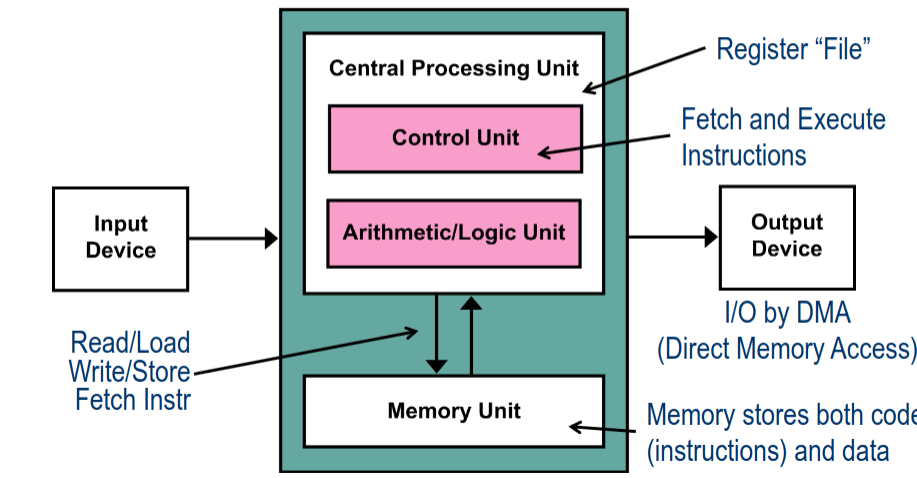
\includegraphics[scale=0.4]{img/von_neumann_arch.png}
  \caption{von Neumann Architecture} 
  \label{fig:von_neumann_arch}
\end{figure}

We will go through these one by one, touching on C and Assembly along the way, but the implementation of these things can differ by the \textbf{computer architecture}, so let's list some of the basic ones. 

\begin{definition}[Computer Architecture]
  The \textbf{computer architecture} is the design of the computer, which includes the CPU, memory, and I/O system. There are many different architectures, but we will focus on the most common ones.
\end{definition}

We first go over some basic theoretical properties of basic data types, focusing on C, and then we cover all the stuff about memory and then all the stuff about the CPU. This is a natural progression since to work with data, you must first know where to store the data and how it is stored (the memory), and then you want to know how data is manipulated (the CPU). 

\section{Computers}

  A computer has many parts which are worth remembering. 

  \begin{definition}
  The 5 main parts of a computer is: 
  \begin{enumerate}
      \item The \textbf{Solid State Drive (SSD)} (or an older version is \textbf{HDD}) is where the computer's long term memory is stored. Most computers usually have 256GB, 512GB, or 1TB of storage. 
      
      \item The \textbf{Random Access Memory (RAM)} is where the computer's short term memory is stored, which is usually 4GB, 8GB, 16GB, or 32GB. The RAM determines how well your computer can work with multiple things running at the same time (applications, browser tabs, ...). Accessing this memory is about 20~100 times faster than accessing the SSD memory. 
      
      \item The \textbf{processor}, or \textbf{Central Processing Unit (CPU)}, is the circuitry that executes instructions that make up a computer program. At the hardware level, a CPU is an \textbf{integrated circuit}, or a \textbf{chip}. This means that a CPU integrates billions of circuits into a chip, where each circuit is really just logic gate (AND, OR, NOT, etc.) made up of a transistor. We can see this in layers: 
      \[\text{CPU Chip} \implies \text{Circuit} \implies \text{Logic Gate} \implies \text{Transistor}\]
      They’re effectively minute gates that switch on or off, thereby conveying the ones or zeros that translate into everything you do with the device. One of the most common advancements of CPU technology is in making those transistors smaller and smaller, where the rate of improvement is referred to as \textit{Moore's Law}. 
      
      In simplest terms, the CPU takes instructions from a program/application and performs a calculation. It first \textit{fetches} the instruction from RAM, \textit{decodes} what the instruction actually is, and then executes the instruction using relevant parts of the CPU. The CPU performs basic arithmetic, logic, controlling, and input/output (I/O) operations specified by the instructions in the program. 
      
      Originally, CPUs had a single processing core. Today’s modern CPU consists of multiple cores that allow it to perform multiple instructions at once, effectively cramming several CPUs on a single chip. Almost all CPUs sold today are at least dual-core or quad-core. Additionally, a physical CPU core can perform two lines of execution (threads) at once with a process called \textit{multithreading}. The clock speed should also be noted with CPUs: the gigahertz figure quoted on the CPU. It denotes how many instructions a CPU can handle per second (giga=billions, mega=millions). 
      
      \item The \textbf{Graphic Processing Unit (GPU)} is a specialized electronic circuit designed to rapidly manipulate and alter memory to accelerate the creation of images intended for output to a display device. 
      
      \item The \textbf{kernel} is a computer program at the core of a computer's operating system that has complete control over everything in the system. It facilitates interactions between hardware and software components. On most systems, the kernel is one of the first programs loaded on startup. It handles the rest of startup as well as memory, peripherals, and input/output (I/O) requests from software, translating them into data-processing instructions for the central processing unit.
      \[CPU, Memory, Devices \iff Kernel \iff Applications\]
      The critical code of the kernel is usually loaded into a separate area of memory, which is protected from access by application programs or other, less critical parts of the operating system. The kernel performs its tasks, such as running processes, managing hardware devices such as the hard disk, and handling interrupts, in this protected \textbf{kernel space}. In contrast, application programs like browsers, word processors, or audio or video players use a separate area of memory, \textbf{user space}. 
  \end{enumerate}
  All components of a computer communicate through a circuit board called the \textbf{motherboard}. 
  \end{definition}

  Note that all of these parts work in conjunction. For the CPU to function, it still must feed to specialized hardware the numbers they need to function. It needs to tell the graphics card to show an explosion or tell the hard drive to transfer a document to the system’s RAM for quicker access.

  \begin{definition}
  Other parts of the computer include: 
  \begin{enumerate}
      \item The \textbf{heatsink} is a passive heat exchanger that transfers heat. It is typically a metallic part which can be attached to a device releasing energy in the form of heat, with the aim of dissipating that heat to a surrounding fluid in order to prevent the device overheating. 
  \end{enumerate}
  \end{definition}

  Certain microcomputers with all these parts (but not packaged) include the \textbf{Raspberry Pi} and the \textbf{Arduino}. 

  \begin{definition}
  A computer processes bits of information based off of how much electricity is traveling through a wire. Since there can be varying amounts of electricity running through a wire, engineers use the transistor as a "switch" that turns on when the voltage running through the wire is greater than the \textit{threshhold voltage}. 
  \end{definition}

  For example, a transistor with a threshhold voltage of 4.5V will turn on when there is a current of at least 4.5V running through the wire and off otherwise. 

  \begin{definition}
  A \textbf{daemon} is a type of program on Unix-like operating systems that runs unobtrusively in the background, rather than under direct control of a user, waiting to be activated. 
  \end{definition}

\section{Representation of Data}

  The inputs of a computational program at its most fundamental level really takes in a \textbf{binary string} of $0$s and $1$s. Note that the choice of $0$ and $1$ is for convenience, but it must be binary (i.e. Boolean) in some way in order for the model to be physically implemented by transistors. Once information is in digital form, we can \textit{compute} over it and gain insights from data that were not accessible in prior times. In fact, we can represent an unbounded variety of objects using only two symbols 0 and 1. 

  Therefore, when we say that a program $P$ takes $x$ as an input, we really mean that $P$ takes as input the \textit{representation of $x$} as a binary string.  

  \begin{definition}
  A \textit{representation scheme} is a way to map an object $x$ to a unique binary string $E(x) \in \{0,1\}^*$. That is, given a set of objects, $E$ is an injective (not not necessarily surjective) map
  \[E: X \longrightarrow \{0,1\}^*\]
  \end{definition}

  \subsection{Representation of Numbers}
  \begin{definition}[Representation of the Naturals]
  A representation for natural numbers (note that in this context, $0 \in \mathbb{N}$) is the (non-surjective) regular binary representation denoted
  \[NtS: \mathbb{N} \longrightarrow \{0,1\}^* \;\;\;\; (NtS= \text{ "Naturals to Strings"})\]
  recursively defined as 
  \[NtS(n) = \begin{cases}
  0 & n = 0 \\
  1 & n = 1 \\
  NtS(\left \lceil{n/2}\right \rceil parity(n) & n > 1 
  \end{cases}\]
  where given strings $x, y \in \{0,1\}^*$, $xy$ denotes the concatenation of $x$ and $y$, and $parity: \mathbb{N} \longrightarrow \{0,1\}^*$ is defined 
  \[parity(n) = \begin{cases}
  0 & n $\text{ is even}$ \\
  1 & n $\text{ is odd}$
  \end{cases}\]
  Since $NtS$ in injective, its inverse $StN: \im{NtS} \subset \{0,1\}^* \longrightarrow \mathbb{N}$ is well-defined. 
  \end{definition}

  \begin{definition}[Representation of the Integers]
  To construct a representation scheme for $\mathbb{Z}$, we can just add one more binary digit to represent the sign of the number. The binary representation $ZtS: \mathbb{Z} \longrightarrow \{0, 1\}^*$ is defined
  \[ZtS(m) = \begin{cases}
  0\, NtS(m) & m \geq 0 \\
  1 \, NtS(-m) & m < 0
  \end{cases}\]
  where $NtS$ is defined as before. Again this function must be injective but need not be surjective. 
  \end{definition}

  When representing rational numbers, we cannot simply concatenate the numerator and denominator as such
  \[a/b \mapsto ZtS(a) \, ZtS(b)\]
  since this map is not surjective (and may overlap with other integers). 

  \begin{definition}[Representation of Rationals]
  To represent a rational number $a/b$, we create a separator symbol $|$ and map the rational number as below in the alphabet $\{0, 1, |\}$. 
  \[q: a/b \mapsto ZtS(a) | ZtS(b)\]
  Then, we use a second map that goes through each digit in $z$ and is defined 
  \[p: \{0, 1, |\} \longrightarrow \{00,11,01\} \subset \{0, 1\}^2, \; p(n) = \begin{cases}
  00 & n = 0 \\
  11 & n = 1 \\
  01 & n = |
  \end{cases}\]
  Therefore, $p$ maps the length $n$ string $z \in \{0, 1\}^*$ to the length $2n$ string $\omega \in \{0, 1\}^*$. The representation scheme for $\mathbb{Q}$ is simply 
  \[QtS \equiv p \circ q\]
  \end{definition}

  \begin{example}
  Given the rational number $-5/8$,
  \[\frac{-5}{8} \mapsto 1101|01000 \mapsto 11110011010011000000\]
  \end{example}

  This same idea of using separators and compositions of injective functions can be used to represent arbitrary $n$-tuples of strings (since a finite Cartesian product of countable sets is also countable). 

  \begin{theorem}[Representation of Vectors]
  All vectors over the field $\mathbb{Q}$ are representable. 
  \end{theorem}
  \begin{proof}
  We can simply create another separator symbol $\cdot$ and have the initial mapping $q$ map to a string over the alphabet $\{0, 1, |, \cdot\}$, which injectively maps to $\{00, 01, 10, 11\}$. 
  \end{proof}

  \begin{corollary}[Representation of Matrices and Tensors]
  Matrices (over $\mathbb{Q}$), which are a collection of vectors are representable in binary. Furthermore, general tenors over the field $\mathbb{Q}$ are representable in binary. 
  \end{corollary}
  \begin{proof}
  Create more separator symbols and map them to a sufficiently large set (which can be extended arbitrarily). For example, to perhaps $\{000, 001, ..., 111\}$. 
  \end{proof}

  \begin{corollary}[Representation of Graphs]
  Directed graphs, which can be represented with their adjacency matrices, can therefore be represented with binary strings. 
  \end{corollary}

  \begin{theorem}[Representation of Images]
  Every finite-resolution image can be represented as a binary number. 
  \end{theorem}
  \begin{proof}
  Since we can interpret each image as a matrix where each element (a pixel) is a color, and since each color can be represented as a 3-tuple of rational numbers corresponding to the intensities of red, green, and blue (for humans, we can restrict it to three primary colors), all images can eventually be decomposed into binary strings. 
  \end{proof}

  \begin{theorem}[Representation of Reals]
  There exists no representation of the reals
  \[NtR: \mathbb{R} \longrightarrow \{0, 1\}^*\]
  \end{theorem}
  \begin{proof}
  By Cantor's theorem, the reals are uncountable. That is, there does not exist a surjective function $NtR: \mathbb{N} \longrightarrow \mathbb{R}$. The implies the nonexistence of an injective inverse; that is, there does not exist an injective function 
  \[RtS: \mathbb{R} \longrightarrow \{0,1\}^*\]
  \end{proof}

  However, since $\mathbb{Q}$ is dense in $\mathbb{R}$, we can approximate every real number $x$ by a rational number $a/b$ to arbitrary accuracy. There are multiple ways to construct these approximations (decimal approximation up to $k$th digit, finite continued fractions, truncated infinite series, etc.), but computers use the \textit{floating-point approximation}. 

  \begin{definition}[Floating-Point Representation]
  The \textbf{floating-point representation scheme} of a real number $x \in \mathbb{R}$ is its approximation as a number of the form 
  \[\sigma b \cdot 2^e\]
  where $\sigma \in \{0, 1\}$ determines the sign of the representation of $x$, $e$ is a (potentially negative) integer, and $b$ is a rational number between $1$ and $2$ expressed as a binary fraction 
  \[1.b_0 b_1 b_2 ... b_k = 1 + \frac{b_1}{2} + \frac{b_2}{4} + ... + \frac{b_k}{2^k}, \;\; b_i \in \{0,1\}\]
  where the number $k$ is fixed (determined by the desired accuracy; greater $k$ implies more digits and better accuracy). The $\sigma b \cdot 2^e$ closest to $x$ is the \textit{floating-point representation}, or \textit{approximation}, of $x$. We can think of $\sigma$ determining the sign, $e$ the order of magnitude (in base 2) of $x$, and $b$ the value of the number scaled down to a value in $[1,2)$, called the \textit{mantissa}. 
  \end{definition}

  \subsection{Representation of General Sets}
  Let there exist some set $\mathcal{O}$ consisting of objects. Then, a representation scheme for representing objects in $\mathcal{O}$ consists of an \textit{encoding} function that maps an object in $\mathcal{O}$ to a string, and a \textit{decoding} function that decodes a string back to an object in $\mathcal{O}$. 

  \begin{definition}
  Let $\mathcal{O}$ be any set. A \textit{representation scheme for $\mathcal{O}$} is a pair of functions $E, D$ where 
  \[E: \mathcal{O} \longrightarrow \{0,1\}^*\]
  is an injective function, and the induced mapping $D$ is restriction of the inverse of $E$ to the image of $E$. 
  \[D: \im(E) \subset \{0,1\}^* \longrightarrow \mathcal{O}\]
  This means that $(D \circ E) (o) = o$ for all $o \in \mathcal{O}$. $E$ is known as the \textit{encoding function} and $D$ is known as the \textit{decoding function}. 
  \end{definition}

  \subsubsection{Prefix-free Encoding}
  \begin{definition}[Prefix]
  For two strings $y, y^\prime$, $y$ is a prefix of $y^\prime$ if $y^\prime$ "starts" with $y$. That is, $y$ is a \textbf{prefix} of $y^\prime$ if $|y| \leq |y^\prime|$ and for every $i<|y|$, $y_i^\prime = y_i$. 
  \end{definition}

  With this, we can define the concept of prefix free encoding. 

  \begin{definition}
  Let $\mathcal{O}$ be a nonempty set and $E: \mathcal{O} \longrightarrow \{0,1\}^*$ be a function. $E$ is \textbf{prefix-free} if $E(o)$ is nonempty for every $o \in \mathcal{O}$ and there does not exist a distinct pair of objects $o, o^\prime \in \mathcal{O}$ such that $E(o)$ is a prefix of $E(o^\prime)$. 
  \end{definition}

  Being prefix-free is a nice property that we would like an encoding to have. Informally, this means that no string $x$ representing an object $o$ is an initial substring of string $y$ representing a different object $o$. This means that we can simply represent a \textit{list} of objects simply by concatenating the representations of all the list members and still get a valid, injective representation. We formalize this below.

  \begin{theorem}
  Suppose that $E: \mathcal{O} \longrightarrow \{0,1\}^*$ is prefix free. Then the following map 
  \[\overline{E}: \mathcal{O}^* \longrightarrow \{0,1\}^*\]
  over all finite length tuples of elements in $\mathcal{O}$ is injective, where for every $o_0, o_1, ..., o_{k-1} \in \mathcal{O}^*$, we define $\overline{E}$ to be the simple concatenation of the separate encodings of $o_i$: 
  \[\overline{E} (o_0, ..., o_{k-1}) \equiv E(o_0) E(o_1) ... E(o_{k-1})\]
  \end{theorem}

  Even if the representation $E$ of objects in $\mathcal{O}$ is prefix free, this does not imply that our representation $\overline{E}$ of \textit{lists} of such objects will be prefix free as well. In fact, it won't be, since for example, given three objects $o, o^\prime, o^{\prime\prime}$, the representation of the list $(o, o^\prime)$ will be a prefix of the representation of the list $(o, o^\prime, o^{\prime\prime})$.

  However, it turns out that in fact we can transform \textit{every} representation into prefix free form, and so will be able to use that transformation if needed to represents lists of lists, lists of lists of lists, and so on. 

  Some natural representations are prefix free. For example, every \textit{fixed output length} representation (i.e. an injective function $E: \mathcal{O} \longrightarrow \{0,1\}^n$) is automatically prefix-free, since a string $x$ can only be a prefix of an equal length $x^\prime$ if $x$ and $x^\prime$ are identical. Moreover, the approach that was used for representing rational numbers can be used to show the following lemma. 

  \begin{lemma}
  Let $E: \mathcal{O} \longrightarrow \{0,1\}^*$ be a one-to-one function. Then there is a one-to-one prefix-free encoding $\overline{E}$ such that 
  \[| \overline{E}(o)| \leq 2 | E(o)| + 2\]
  for every $o \in \mathcal{O}$. 
  \end{lemma}
  \begin{proof}
  The general idea is the use the map $0 \mapsto 00$, $1 \mapsto 11$ to "double" every bit in the string $x$ and then mark the end of the string by concatenating to it the pair $01$. If we encode a string $x$ in this way, it ensures that the encoding of $x$ is never a prefix of the encoding of a distinct string $x^\prime$. (Note that this is not the only or even the best way to transform an arbitrary representation into prefix-free form.)
  \end{proof}

  \subsection{Representing Letters and Text}
  We can represent a letter or symbol by a string, and then if this representation is prefix free, we can represent a sequence of symbols by merely concatenating the representation of each symbol. Here are a few examples. 

  \subsubsection{ASCII}

  The \textbf{ASCII} (also called US-ASCII) code, which stands for American Standard Code for Information Interchange is a $7$ bit character code where every single bit represents a unique character. ASCII codes represent text in computers, telecommunications equipment, and other devices. Most modern character-encoding schemes are based on ASCII, although they support many additional characters.

  The first 32 characters are called the \textit{control characters}: codes originally intended not to represent printable information, but rather to control devices (such as printers) that make use of ASCII, or to provide meta-information about data streams. For example, character 10 (decimal) represents the "line feed" function (which causes a printer to advance its paper) and character 8 represents "backspace." Except for the control characters that prescribe elementary line-oriented formatting, ASCII does not define any mechanism for describing the structure or appearance of text within a document. 
  \begin{center}
  \scalebox{0.8}{%
  \begin{tabular}{ |c|c|c|c|c|l| } 
  \hline
  Dec & Oct & Hex & Bin & Symbol & Description\\ 
  \hline
  0 & 000& 00& 0000000 & NULL & Null char\\ 
  1 & 001&01&0000001 & SOH & Start of Heading \\
  2 & 002 & 02 & 0000010& STX & Start of Text \\
  3 & 003 & 03 & 0000011&ETX & End of Text \\
  4 & 004 & 04 & 0000100 & EOT & End of Transmission \\
  5 & 005 & 05 & 0000101 & ENQ & Enquiry \\
  6 & 006 & 06 & 0000110 & ACK & Acknowledgement \\
  7 & 007 & 07 & 0000111 & BEL & Bell \\
  8 & 010 & 08 & 0001000 & BS & Back Space\\
  9 & 011 & 09 & 0001001 & HT & Horizontal Tab \\
  10 & 012 & 0A & 0001010 & LF & Line Feed \\
  11 & 013 & 0B & 0001011 & VT & Vertical Tab \\
  12 & 014 & 0C & 0001100 & FF & Form Feed\\
  13 & 015 & 0D & 0001101 & CR & Carriage Return \\
  14 & 016 & 0E & 0001110 & SO & Shift Out/X-On\\
  15 & 017 & 0F & 0001111 & SI & Shift In/X-Off\\
  16 & 020 & 10 & 0010000 & DLE & Data Line Escape\\
  17 & 021 & 11 & 0010001 & DC1 & Device Control 1\\
  18 & 022 & 12 & 0010010 & DC2 & Device Control 2\\
  19 & 023 & 13 & 0010011 & DC3 & Device Control 3\\
  20 & 024 & 14 & 0010100 & DC4 & Device Control 4 \\
  21 & 025 & 15 & 0010101 & NAK & Negative Acknowledgement\\
  22 & 026 & 16 & 0010110 & SYN & Synchronous Idle \\
  23 & 027 & 17 & 0010111 & ETB & End of Transmit Block\\
  24 & 030 & 18 & 0011000 & CAN & Cancel\\
  25 & 031 & 19 & 0011001 & EM & End of Medium\\
  26 & 032 & 1A & 0011010 & SUB & Substitute\\
  27 & 033 & 1B & 0011011 & ESC & Escape\\
  28 & 034 & 1C & 0011100 & FS & File Separator \\
  29 & 035 & 1D & 0011101 & GS & Group Separator\\
  30 & 036 & 1E & 0011110 & RS & Record Separator \\
  31 & 037 & 1F & 0011111 & US & Unit Separator\\
  \hline
  \end{tabular}}
  \end{center}

  The rest of the characters are the ASCII printable characters. 

  \scalebox{0.8}{%
  \begin{tabular}{ |c|c|c|c|c|l|c|c|c|c|c|l| } 
   \hline
  Dec & Oct & Hex & Bin & Sym & Description & Dec & Oct & Hex & Bin & Sym & Description \\
   \hline
  32 & 040 & 20& 0100000 &   & Space & 80 & 120 & 50& 1010000 &P&Uppercase P\\
  33 & 041 & 21& 0100001 & ! & Exclamation & 81 & 121 & 51& 1010001 &Q&Uppercase Q\\
  34 & 042 & 22& 0100010 & " & Double quotes & 82 & 122 & 52& 1010010 &R&Uppercase R\\
  35 & 043 & 23& 0100011 & \# & Number & 83 & 123 & 53& 1010011 &S&Uppercase S\\
  36 & 044 & 24& 0100100 & \$ & Dollar & 84 & 124 & 54& 1010100 &T&Uppercase T\\
  37 & 045 & 25& 0100101 & \% & Per cent sign & 85 & 125 & 55& 1010101 &U&Uppercase U\\
  38 & 046 & 26& 0100110 & \& & Ampersand & 86 & 126 & 56& 1010110 &V&Uppercase V\\
  39 & 047 & 27& 0100111 & ' &Single quote & 87 & 127 & 57& 1010111 &W&Uppercase W\\
  40 & 050 & 28& 0101000 & ( & Open paren.& 88 & 130 & 58& 1011000 &X&Uppercase X\\
  41 & 051 & 29& 0101001 & ) & Closed paren.& 89 & 131 & 59& 1011001 &Y&Uppercase Y\\
  42 & 052 & 2A& 0101010 & * & Asterisk & 90 & 132 & 5A& 1011010 &Z&Uppercase Z\\
  43 & 053 & 2B& 0101011 & + & Plus & 91 & 133 & 5B& 1011011 & [ & Opening bracket\\
  44 & 054 & 2C& 0101100 & , & Comma & 92 & 134 & 5C& 1011100 & \textbackslash & Backslash\\
  45 & 055 & 2D& 0101101 & - & Hyphen & 93 & 135 & 5D& 1011101 & ] & Closing bracket\\
  46 & 056 & 2E& 0101110 & . &Period & 94 & 136 & 5E& 1011110 & \string^ & Caret\\
  47 & 057 & 2F& 0101111 & / & Slash & 95 & 137 & 5F& 1011111 & \_ & Underscore\\
  48 & 060 & 30& 0110000 & 0 & Zero & 96 & 140 & 60& 1100000 &`&Grave accent\\
  49 & 061 & 31& 0110001 & 1 & One & 97 & 141 & 61& 1100001 &a& Lowercase a\\
  50 & 062 & 32& 0110010 & 2 & Two & 98 & 142 & 62& 1100010 &b&Lowercase b\\
  51 & 063 & 33& 0110011 & 3 & Three & 99 & 143 & 63& 1100011 &c&Lowercase c\\
  52 & 064 & 34& 0110100 & 4 & Four & 100 & 144 & 64& 1100100 &d&Lowercase d\\
  53 & 065 & 35& 0110101 & 5 & Five & 101 & 145 & 65& 1100101 &e&Lowercase e\\
  54 & 066 & 36& 0110110 & 6 & Six & 102 & 146 & 66& 1100110 &f&Lowercase f\\
  55 & 067 & 37& 0110111 & 7 & Seven & 103 & 147 & 67 &1100111 &g&Lowercase g\\
  56 & 070 & 38& 0111000 & 8 & Eight & 104 & 150 & 68& 1101000 &h&Lowercase h\\
  57 & 071 & 39& 0111001 & 9 & Nine & 105 & 151 & 69& 1101001 &i&Lowercase i\\
  58 & 072 & 3A& 0111010 & : & Colon & 106 & 152 & 6A& 1101010 &j&Lowercase j\\
  59 & 073 & 3B& 0111011 & ; & Semicolon & 107 & 153 & 6B& 1101011 &k&Lowercase k\\
  60 & 074 & 3C& 0111100 & < & Less than & 108 & 154 & 6C& 1101100 &l&Lowercase l\\
  61 & 075 & 3D& 0111101 & = & Equals & 109 & 155 & 6D& 1101101 &m&Lowercase m\\
  62 & 076 & 3E& 0111110 & > & Greater than & 110 & 156 & 6E& 1101110 &n&Lowercase n\\
  63 & 077 & 3F& 0111111 & ? & Question mark & 111 & 157 & 6F& 1101111 &o&Lowercase o\\
  64 & 100 & 40& 1000000 & @ & At symbol & 112 & 160 & 70& 1110000 &p&Lowercase p\\
  65 & 101 & 41& 1000001 & A & Uppercase A & 113 & 161 & 71& 1110001 &q&Lowercase q\\
  66 & 102 & 42& 1000010 & B& Uppercase B & 114 & 162 & 72& 1110010 &r&Lowercase r\\
  67 & 103 & 43& 1000011 &C&Uppercase C & 115 & 163 & 73& 1110011 &s&Lowercase s\\
  68 & 104 & 44& 1000100 &D&Uppercase D & 116 & 164 & 74& 1110100 &t&Lowercase t\\
  69 & 105 & 45& 1000101 &E&Uppercase E & 117 & 165 & 75& 1110101 &u&Lowercase u\\
  70 & 106 & 46& 1000110 &F&Uppercase F & 118 & 166 & 76& 1110110 &v&Lowercase v\\
  71 & 107 & 47& 1000111 &G&Uppercase G & 119 & 167 & 77& 1110111 &w&Lowercase w\\
  72 & 110 & 48& 1001000 &H&Uppercase H & 120 & 170 & 78& 1111000 &x&Lowercase x\\
  73 & 111 & 49& 1001001 &I&Uppercase I & 121 & 171 & 79& 1111001 &y&Lowercase y\\
  74 & 112 & 4A& 1001010 &J&Uppercase J & 122 & 172 & 7A& 1111010 &z&Lowercase z\\
  75 & 113 & 4B& 1001011 &J&Uppercase K & 123 & 173 & 7B& 1111011 &\{& Opening brace\\
  76 & 114 & 4C& 1001100 &L&Uppercase L & 124 & 174 & 7C& 1111100 &|& Vertical bar\\
  77 & 115 & 4D& 1001101 &M&Uppercase M & 125 & 175 & 7D& 1111101 &\}& Closing brace\\
  78 & 116 & 4E& 1001110 &N&Uppercase N & 126 & 176 & 7E& 1111110 & $\sim$ & Tilde\\
  79 & 117 & 4F& 1001111 &O&Uppercase O & 127 & 177 & 7F& 1111111 & & Delete\\
   \hline
  \end{tabular}}

  \subsubsection{Extended ASCII}
  The \textbf{Extended ASCII} (EASCII or high ASCII) character encodings are 8-bit or larger encodings that include the standard 7-bit ASCII characters, plus additional characters. Note that this does not mean that the standard ASCII coding has been updated to include more than 128 characters nor does it mean that there is an universal extension to the original ASCII coding. In fact, there are several (over 100) extended ASCII encodings. 

  With the creation of the 7-bit ASCII format, increased need for more letters and symbols (such as characters in other languages or more punctuation/mathematical symbols). With better computers and software, it became obvious that they could handle text that uses 256-character sets at almost no additional cost in programming or storage. The 8-bit format would allow ASCII to be used unchanged and provide 128 more characters. 

  But even 256 characters is still not enough to cover all purposes, all languages, or even all European languages, so the emergence of \textit{many} ASCII-derived 8-bit character sets was inevitable. Translating between these sets (\textit{transcoding}) is complex, especially if a character is not in both sets and was often not done, producing \textbf{mojibake} (semi-readable text resulting from text being decoded using an unintended character encoding. The result is a systematic replacement of symbols with completely unrelated ones, often from a different writing system). ASCII can also be used to create graphics, commonly called \textbf{ASCII art}. 

  But ASCII isn't enough. We have lots of languages with lots of characters that computers should ideally display. Unicode assigns each character a unique number, or code print. Computers deal with such numbers as bytes: 8-bit computers would treat an 8-bit byte as the largest numerical unit easily represented on the hardware, 16-bit computers would expand that to 2 bytes, and so forth. Old character encodings like ASCII are from the (pre-) 8-bit era, and try to cram the dominant language in computing at the time, i.e. English, into numbers ranging from 0 to 127 (7 bits). When ASCII got extended by an 8th bit for other non-English languages, the additional 128 numbers/code points made available by this expansion would be mapped to different characters depending on the language being displayed. The \textbf{ISO-8859} standards are the most common forms of this mapping: 
  \begin{enumerate}
      \item \textbf{ISO-8859-1}
      \item \textbf{ISO-8859-15}, also called \textbf{ISO-Latin-1}
  \end{enumerate}
  But that's not enough when you want to represent characters from more than one language, so cramming all available characters into a single byte just won't work. The following shows ways to do this (that is compatible with ASCII). 

  \subsubsection{ISO-10646, UCS}
  We can simply expand the value range by adding more bits. The UCS-2 uses 2 bytes (or 16 bits) and UCS-4 uses 4 bytes (32 bits). However, these codings suffer from inherently the same problem as ASCII and ISO-8859 standards, as their value range is still limited, even if the limit is vastly higher. Note that these encode from the ISO-10646, which defines several character encoding forms for the Universal Coded Character Set. 
  \begin{enumerate}
      \item UCS-2 can store $2^{16} = 65,536$ characters. 
      \item UCS-4 can store $2^{32} = 4,294,967,296$ characters. 
  \end{enumerate}
  Notice that UCS encoding has a fixed number of bytes per character, which means that UCS-2 stores each character in 2 bytes, and UCS-4 stores each character in 4 bytes. This is different from \textbf{UTF-8} encoding. 

  ISO 10646 and Unicode have an identical repertoire and numbers—the same characters with the same numbers exist on both standards, although Unicode releases new versions and adds new characters more often. Unicode has rules and specifications outside the scope of ISO 10646. ISO 10646 is a simple character map, an extension of previous standards like ISO 8859. In contrast, Unicode adds rules for collation, normalization of forms, and the bidirectional algorithm for right-to-left scripts such as Arabic and Hebrew. For interoperability between platforms, especially if bidirectional scripts are used, it is not enough to support ISO 10646; Unicode must be implemented.


  \subsubsection{Unicode, UTF-8}
  Unicode is the universal character encoding, maintained by Unicode Consortium, and it covers the characters for all the writing systems of the world, modern and ancient. It also includes technical symbols, punctuation, and many other characters used in writing text. As of Unicode Version 13.0, the Unicode standard contains 143,859 characters, stored in the format U+****, where **** is a number in hexadecimal notation. Notice that these ones are not fixed in the number of bits; that is, 
  \[\text{U+27BD and U+1F886}\]
  are perfectly viable representations of characters in Unicode. Even though only 143,859 characters are in use, Unicode currently allows for 1,114,112 ($16^5 + 16^4$) code values, and assigns codes covering nearly all modern text writing systems, as well as many historical ones and for many non-linguistic characters such as printer's dingbats, mathematical symbols, etc.

  \textit{Note that Unicode, along with ISO-10646, is a standard that assigns a name and a value (\textbf{Character Code} or \textbf{Code-Point}) to each character in its repertoire.} However, the Unicode format must be encoded in a binary format for the computer to understand. When you save a document, the text editor has to explicitly set its encoding to be UTF-8 (or whatever other format) the user wants it to be. Also, when a text editor program reads a file, it needs to select a text encoding scheme to decode it correctly. Even further, when you are typing and entering a letter, the text editor needs to know what scheme you use so that it will save it correctly. Therefore, \textit{UTF-8 encoding is a way to represent these characters digitally in computer memory.} The way that \textbf{UTF-8} encodes characters is with the following format:
  \begin{lstlisting}
  1st Byte    2nd Byte    3rd Byte    4th Byte    Number of Free Bits   
  0xxxxxxx                                                7             
  110xxxxx    10xxxxxx                                (5+6)=11          
  1110xxxx    10xxxxxx    10xxxxxx                  (4+6+6)=16         
  11110xxx    10xxxxxx    10xxxxxx    10xxxxxx    (3+6+6+6)=21         
  \end{lstlisting}
  From this, we can see that UTF-8 uses a variable number of bytes per character. All UTF encodings work in roughly the same manner: you choose a unit size, which for UTF-8 is 8 bits, for UTF-16 is 16 bits, and for UTF-32 is 32 bits. The standard then defines a few of these bits as \textit{flags} (e.g. the 0, 110, 1110, 11110, ...). If they're set, then the next unit in a sequence of units is considered part of the same character. If they're not set, this unit represents one character fully. Thus, the most common (English) characters only occupy one byte in UTF-8 (two in UTF-16, 4 in UTF-32), but other language characters can occupy more bytes. We can see that UTF-8 can encode up to (and slightly more than) $2^{21} = 2,097,152$ characters. UTF-8 is by far the most common encoding for the World Wide Web, accounting for 96.0\% of all web pages, and up to 100\% for some languages, as of 2021.

  For example, let's take a random character, say with the Unicode value to be U+6C49. Then, we convert this to binary to get
  \[\text{01101100 01001001}\]
  But we can't just store this because this isn't a prefix-free notation. This is when UTF-8 is needed. Using the chart above, we need to prefix our character with some headers/flags. The binary Unicode value of the character is 16 bits long, so we can store it in 3 bytes (in the format of the third row) as it provides enough space. The headers are not bolded, while the binary values added are. 
  \[\text{1110}\textbf{0110} \; \text{10}\textbf{110001} \; \text{10}\textbf{001001}\]
  We can take another example of a character with the Unicode value U+1F886. Converting to binary gets
  \[\text{0001 1111 1000 1000 0110}\]
  There are 20 bits, so we will need to store it in 4 bytes (in the format of fourth row) as it provides enough space (21). We convert the 20-bit-long binary Unicode value to a 21-bit-long value (so that it is compatible with the 21 free bits) to get
  \[\text{0 0001 1111 1000 1000 0110}\]
  Encoding it in UTF-8 in 4 bytes gives
  \[\text{11110}\textbf{000} \; \text{10}\textbf{011111} \;  \text{10}\textbf{100010} \; \text{10}\textbf{000110}\]
  There is no need to go beyond 4 bytes since every Unicode value will have at most 5 hexadecimal digits (since $16^5 = 1,048,576$, which is far more than the number of characters there are). There is also another, obsolete, encoding used called the \textbf{UTF-7}. 

  Both the UCS and UTF standards encode the code points as defined in Unicode. In theory, those encodings could be used to encode any number (within the range the encoding supports) - but of course these encodings were made to encode Unicode code points. Windows handles so-called "Unicode" strings as UTF-16 strings, while most UNIXes default to UTF-8 these days. Communications protocols such as HTTP tend to work best with UTF-8, as the unit size in UTF-8 is the same as in ASCII, and most such protocols were designed in the ASCII era. On the other hand, UTF-16 gives the best average space/processing performance when representing all living languages. 

  While UTF-7, 8, 16, and 32 all have the nice property of being able to store \textit{any} code point correctly, there are hundreds of encodings that can only store a set amount of characters. If there’s no equivalent for the Unicode code point you’re trying to represent in the encoding you’re trying to represent it in, you usually get a little question mark: ? For example, trying to store Russian or Hebrew letters in these encodings results in a bunch of question marks. 

  \subsubsection{All Plaintext depends on Encodings}
  Note that \textbf{it does not make sense to have a string without knowing what encoding it uses}. We can't just assume that every plaintext is in ASCII, since there are hundreds of extended ASCII encodings. If you have a string, in memory, in a file, or in an email message, you have to know what encoding it is in or you cannot interpret it or display it to users correctly. 

  For example, when you are sending an email, Gmail is the only client that automatically converts your text to UTF-8, regardless of what you set in the header. The browser also uses a certain encoding, which can be accessed (and changed) under the "view" tab. 

  \subsection{Text Files}
  The ASCII character set is the most common compatible subset of character sets for English-language text files, and is generally assumed to be the default file format in many situations. 

  In the Mac, checking the character encoding of a text file can be done with the command 
  \begin{lstlisting}
  >>>file -I filename.txt
  filename.txt: text/plain; charset=us-ascii
  \end{lstlisting}
  ASCII covers American English, but for the British Pound sign, the Euro sign, or characters used outside English, a richer character set must be used. In many systems, this is chosen based on the default setting on the computer it is read on. Prior to UTF-8, this was traditionally single-byte encodings (such as ISO-8859-1 through ISO-8859-16) for European languages and wide character encodings for Asian languages. However, most computers use UTF-8 as the natural extension. We can check this firsthand by inputting a non-ASCII character in filename.txt, which would result in
  \begin{lstlisting}
  >>>file -I filename.txt
  filename.txt: text/plain; charset=utf-8
  \end{lstlisting}
  Because encodings necessarily have only a limited repertoire of characters, often very small, many are only usable to represent text in a limited subset of human languages. Unicode is an attempt to create a common standard for representing all known languages, and most known character sets are subsets of the very large Unicode character set. Although there are multiple character encodings available for Unicode, the most common is UTF-8, which has the advantage of being backwards-compatible with ASCII; that is, every ASCII text file is also a UTF-8 text file with identical meaning. UTF-8 also has the advantage that it is easily auto-detectable. Thus, a common operating mode of UTF-8 capable software, when opening files of unknown encoding, is to try UTF-8 first and fall back to a locale dependent legacy encoding when it definitely isn't UTF-8.

  Because of their simplicity, text files are commonly used for storage of information. When data corruption occurs in a text file, it is often easier to recover and continue processing the remaining contents. A disadvantage of text files is that they usually have a low entropy, meaning that the information occupies more storage than is strictly necessary. A simple text file may need no additional metadata (other than knowledge of its character set) to assist the reader in interpretation. A text file may contain no data at all, which is a case of zero-byte file.

  \subsubsection{Plain Text, Rich Text}
  \textbf{Plain text} is a loose term for data (e.g. file contents) that represent only characters of readable material but not its graphical representation nor other objects (floating-point numbers, images, etc.). It may also include a limited number of "whitespace" characters that affect simple arrangement of text, such as spaces or line breaks. A plain text file cannot have bold text, fonts, larger font sizes, or any other special text formatting. 

  Plain text is different from \textbf{formatted text} or \textbf{rich text}, where style information is included and structured text, where structral parts of the document such as paragraphs, sections, and the like are identified. 

  Most systems associate plain text file with the file .txt. To view a plaintext file, a text editor must be used. 

  \subsection{Binary Files}
  Another type of data is a \textbf{binary file}, which is a computer file that is not a text file (it is often used as a term meaning \textit{non-text file}). Many binary file formats contain parts that can be interpreted as text; for example, some computer document files containing formatted text, such as older Microsoft Word document files, contain the text of the document but also contain formatting information in binary form.

  Binary files are usually thought of as being a sequence of bytes, which means the binary digits (bits) are grouped in eights. Binary files typically contain bytes that are intended to be interpreted as something other than text characters. Compiled computer programs are typical examples; indeed, compiled applications are sometimes referred to, particularly by programmers, as binaries. But binary files can also mean that they contain images, sounds, compressed versions of other files, etc. – in short, any type of file content whatsoever.

  \subsubsection{Viewing Binary Files}
  A hex editor or viewer may be used to view file data as a sequence of hexadecimal (or decimal, binary or ASCII character) values for corresponding bytes of a binary file. 

  If a binary file is opened in a text editor, each group of eight bits will typically be translated as a single character, and the user will see a (probably unintelligible) display of textual characters. If the file is opened in some other application, that application will have its own use for each byte: maybe the application will treat each byte as a number and output a stream of numbers between 0 and 255—or maybe interpret the numbers in the bytes as colors and display the corresponding picture. Other type of viewers (called 'word extractors') simply replace the unprintable characters with spaces revealing only the human-readable text. This type of view is useful for a quick inspection of a binary file in order to find passwords in games, find hidden text in non-text files and recover corrupted documents. It can even be used to inspect suspicious files (software) for unwanted effects. For example, the user would see any URL/email to which the suspected software may attempt to connect in order to upload unapproved data (to steal). If the file is itself treated as an executable and run, then the operating system will attempt to interpret the file as a series of instructions in its machine language

  Standards are very important to binary files. For example, a binary file interpreted by the ASCII character set will result in text being displayed. A custom application can interpret the file differently: a byte may be a sound, or a pixel, or even an entire word. Binary itself is meaningless, until such time as an executed algorithm defines what should be done with each bit, byte, word or block. Thus, just examining the binary and attempting to match it against known formats can lead to the wrong conclusion as to what it actually represents. This fact can be used in \textit{steganography}, where an algorithm interprets a binary data file differently to reveal hidden content. Without the algorithm, it is impossible to tell that hidden content exists.

\section{Encoding Schemes}

  In order to get into memory, it is helpful to know the theory behind how primitive types are stored in memory.  

  \begin{definition}[Collections of Bits]
    There are many words that are used to talk about values of different data types: 
    \begin{enumerate}
      \item A \textbf{bit} (b) is either $0$ or $1$. 
      \item A \textbf{Hex} (x) is a collection of 4 bits, with a total of $2^4 = 16$ possible values, and this is used since it is easy to read for humans. 
      \item A \textbf{Byte} (B) is a collection of 8 bits or 2 hex, with a total of $2^8 = 256$ possible values, and most computers will work with Bytes as the smallest unit of memory. 
    \end{enumerate}
  \end{definition}

  \begin{definition}[Collections of Bytes]
    Sometimes, we want to talk about slightly larger collections, so we group them by how many bytes they have. However, note that these may not always be the stated size, depending on what architecture or language you are using. This is more of a general term, and they may have different names in different languages. If there is a difference, we will state it explicitly. 
    \begin{enumerate}
      \item A \textbf{word} (w) is 2 Bytes. 
      \item A \textbf{long} (l) is 4 Bytes. 
      \item A \textbf{quad} (q) is 8 Bytes. 
    \end{enumerate} 
    Try to know which letter corresponds to which structure, since that will be useful in both C and Assembly. 
  \end{definition}

  \subsection{Booleans and Characters} 

    \begin{definition}[Booleans in C]
      The most basic type is the boolean, which is simply a bit. In C, it is represented as \texttt{bool}, and it is either \texttt{true} (1) or \texttt{false} (0). 
    \end{definition}

    We can manually check the size of the boolean type in C with the following code. 

    \begin{figure}[H]
      \centering 
      \noindent\begin{minipage}{.5\textwidth}
      \begin{lstlisting}[firstnumber=1]{Code}
        #include<stdio.h>
        #include<stdbool.h>

        int main() {
          printf("%lu\n", sizeof(bool)); 
          return 0; 
        }
      \end{lstlisting}
      \end{minipage}
      \hfill
      \begin{minipage}{.49\textwidth}
      \begin{lstlisting}[]{Output}
        1
        .
        .
        .
        .
        .
        .
      \end{lstlisting}
      \end{minipage}
      \caption{We can verify the size of various primitive data types in C with the \texttt{sizeof} operator.} 
      \label{fig:boolean_size}
    \end{figure}

  \subsection{Integer Family}

    The most primitive things that we can store are integers. Let us talk about how we represent some of the simplest primitive types in C: unsigned short, unsigned int, unsigned long, unsigned long long.

    \begin{definition}[Unsigned Integer Types in C]
      In C, there are several integer types. We use this hierarchical method to give flexibility to the programmer on the size of the integer and whether it is signed or not. 
      \begin{enumerate} 
        \item An \textbf{unsigned short} is 2 bytes long and can be represented as a 4-digit hex or 16 bits, with values in $[0:65,535]$. Therefore, say that we have 
        \item An \textbf{unsigned int} is 4 bytes long and can be represented as an 8-digit hex or 32 bits, with values in $[0:4,294,967,295]$. 
        \item An \textbf{unsigned long} is 8 bytes and can be represented as an 16-digit hex or 64 bits, but they are only guaranteed to be stored in 32 bits in other systems. 
        \item An \textbf{unsigned long long} is 8 bytes and can be represented as an 16-digit hex or 64 bits, and they are guaranteed to be stored in 64 bits in other systems. 
      \end{enumerate} 
    \end{definition}

    \begin{theorem}[Bit Representation of Unsigned Integers in C]
      To encode a signed integer in bits, we simply take the binary expansion of it. 
      \begin{figure}[H]
        \centering 
        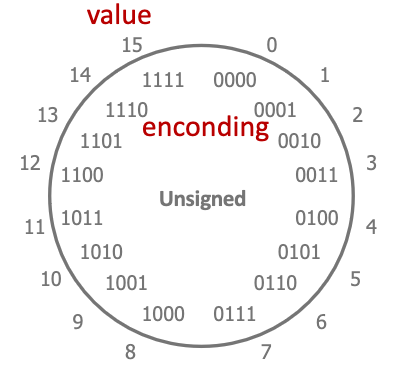
\includegraphics[scale=0.4]{img/unsigned_encoding.png}
        \caption{Unsigned encoding of 4-bit integers in C. } 
        \label{fig:unsigned_encoding}
      \end{figure}
    \end{theorem}

    \begin{example}[Bit Representation of Unsigned Integers in C]
      We can see for ourselves how these numbers are represented in bits. Printing the values out in binary requires to make new functions, but we can easily convert from hex to binary. 

      \noindent\begin{minipage}{.5\textwidth}
      \begin{lstlisting}[]{Code}
        int main() { 

          unsigned short x = 13; 
          unsigned int y = 256;

          printf("%x\n", x);
          printf("%x\n", y);

          return 0; 
        }
      \end{lstlisting}
      \end{minipage}
      \hfill
      \begin{minipage}{.49\textwidth}
      \begin{lstlisting}[]{Output}
        d
        100 
        .
        .
        .
        .
        .
        .
        .
        .
      \end{lstlisting}
      \end{minipage}
    \end{example}

    So far, the process of converting unsigned numbers to bits seemed simple. Now let's introduce signed integers. 

    \begin{definition}[Signed Integer Types in C]
      In C, there are several signed integer types. We use this hierarchical method to give flexibility to the programmer on the size of the integer and whether it is signed or not. 
      \begin{enumerate} 
        \item A \textbf{signed short} is 2 bytes long and can be represented as a 4-digit hex or 16 bits, with values in $[-32,768: 32,767]$. 
        \item A \textbf{signed int} is 4 bytes long and can be represented as an 8-digit hex or 32 bits, with values in $[-2,147,483,648: 2,147,483,647]$. 
        \item A \textbf{signed long} is 8 bytes and can be represented as an 16-digit hex or 64 bits, but they are only guaranteed to be stored in 32 bits in other systems. 
        \item A \textbf{signed long long} is 8 bytes and can be represented as an 16-digit hex or 64 bits, and they are guaranteed to be stored in 64 bits in other systems. 
      \end{enumerate}
    \end{definition}

    To store signed integers, it is intuitive to simply take the first (left-most) bit and have that be the sign. Therefore, we lose one significant figure but gain information about the sign. However, this has some problems: first, there are two representations of zeros: $-0$ and $+0$. Second, the continuity from $-1$ to $0$ is not natural. It is best explained through an example, which doesn't lose much insight into the general case. 

    \begin{example}[Problems with the Signed Magnitude]
      Say that you want to develop the signed magnitude representation for 4-bit integers in C. Then, you can imagine the following diagram to represent the numbers. 
      \begin{figure}[H]
        \centering 
        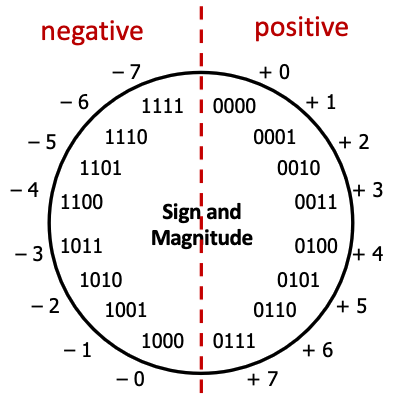
\includegraphics[scale=0.4]{img/signed_magnitude_encoding.png}
        \caption{Signed magnitude encoding of 4-bit integers in C.} 
        \label{fig:signed_magnitude_encoding}
      \end{figure}
      You can see that there are some problems: 
      \begin{enumerate}
        \item There are two representations for $0$, which is 0000 and 1000. 
        \item -1 (1001) plus 1 becomes -2 (1010). 
        \item The lowest number -7 (1111) plus 1 goes to 0 (0000) when it should go to -6 (1100). 
        \item The highest number 7 (0111) plus 1 goes to 0 (1000). 
      \end{enumerate}
    \end{example}

    An alternative way is to use the two's complement representation, which solves both problems and makes it more natural. 

    \begin{theorem}[Bit Representation of Signed Integers in C]
      The \textbf{two's complement} representation is a way to represent signed integers in binary. It is defined as follows. Given that you want to store a decimal number $p$ in $n$ bits, 

      \begin{enumerate}
        \item If $p$ is positive, then take the binary expansion of that number, which should be at most $n-1$ bits (no overflow), pad it with $0$s on the left. 
        \item If $p$ is negative, then you can do two things: First, take the binary expansion of the positive number, flip all the bits, and add 1. Or second, represent $p = q - 2^n$, take the binary representation of $q$ in $n-1$ bits, and add a $1$ to the left. 
      \end{enumerate}
      If you have a binary number $b = b_{n}b_{n-1}\cdots b_1$ then to convert it to a decimal number, you simply calculate 
      \begin{equation}
        q = -b_{n}2^{n-1} + b_{n-1}2^{n-2} + \cdots + b_1
      \end{equation}
      \begin{figure}[H]
        \centering 
        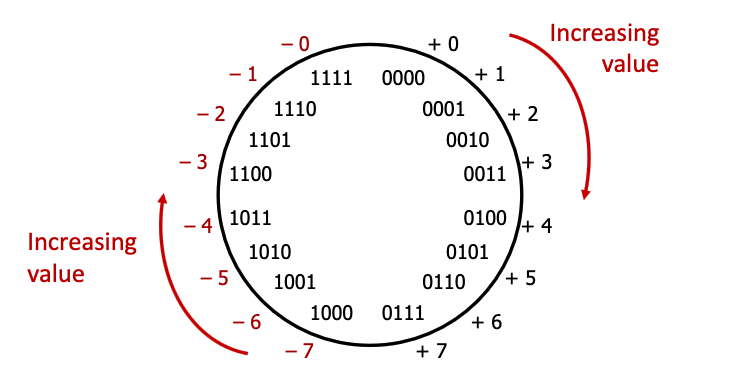
\includegraphics[scale=0.4]{img/twos_complement_encoding.png}
        \caption{Two's complement encoding of 4-bit integers in C.} 
        \label{fig:twos_complement_encoding}
      \end{figure}
    \end{theorem}

    \begin{example}[Bit Representation of Signed Integers in C]
      We can see for ourselves how these numbers are represented in bits. 

      \noindent\begin{minipage}{.5\textwidth}
      \begin{lstlisting}[]{Code}
        int main() { 

          short short_pos = 13; 
          short short_neg = -25; 
          int int_pos = 256;
          int int_neg = -512; 

          printf("%x\n", short_pos);
          printf("%x\n", short_neg);
          printf("%x\n", int_pos);
          printf("%x\n", int_neg);

          return 0; 
        }
      \end{lstlisting}
      \end{minipage}
      \hfill
      \begin{minipage}{.49\textwidth}
      \begin{lstlisting}[]{Output}
        d
        ffe7
        100
        ffffffe00
        .
        .
        .
        .
        .
        .
        .
        .
        .
        .
      \end{lstlisting}
      \end{minipage}
    \end{example}

    \begin{figure}[H]
      \centering 
      \noindent\begin{minipage}{.5\textwidth}
      \begin{lstlisting}[]{Code}
        #include<stdio.h>
        #include<stdbool.h>

        int main() {
          printf("%lu\n", sizeof(bool)); 
          printf("%lu\n", sizeof(short)); 
          printf("%lu\n", sizeof(int)); 
          printf("%lu\n", sizeof(long)); 
          printf("%lu\n", sizeof(long long)); 
          return 0; 
        }
      \end{lstlisting}
      \end{minipage}
      \hfill
      \begin{minipage}{.49\textwidth}
      \begin{lstlisting}[]{Output}
        1
        2
        4
        8
        8
        .
        .
        .
        .
        .
        .
      \end{lstlisting}
      \end{minipage}
      \caption{Size of various integer types in C with the \texttt{sizeof}.} 
      \label{fig:integer_size}
    \end{figure}


    \subsubsection{Arithmetic Operations on Binary Numbers}

      \begin{theorem}[Inversion of Binary Numbers]
        Given a binary number $p$, to compute $-p$, simply invert the bits and add 1.
      \end{theorem}

      \begin{theorem}[Addition and Subtraction of Binary Numbers]
        Given two binary numbers $p$ and $q$. 
        \begin{enumerate}
          \item To compute $p + q$, simply add the numbers together as you would in base 10, but carry over when the sum is greater than 1. 
          \item To compute $p - q$, you can invert $q$ to $-q$ and compute $p + (-q)$. 
        \end{enumerate}
      \end{theorem}

      % TODO: Bitshift and Bitwise Operations

  \subsection{Float Family} 

  \begin{definition}[Floating Point Types in C]
    In C, there are several floating point types. We use this hierarchical method to give flexibility to the programmer on the size of the integer and whether it is signed or not. 
    \begin{enumerate} 
      \item A \textbf{float} is 4 bytes long and can be represented as an 8-digit hex or 32 bits, with values in $[1.2 \times 10^{-38}: 3.4 \times 10^{38}]$. 
      \item A \textbf{double} is 8 bytes long and can be represented as an 16-digit hex or 64 bits, with values in $[2.3 \times 10^{-308}: 1.7 \times 10^{308}]$. 
      \item A \textbf{long double} is 8 bytes and can be represented as an 16-digit hex or 64 bits, but they are only guaranteed to be stored in 80 bits in other systems. 
    \end{enumerate}
  \end{definition}

  \begin{theorem}[Bit Representation of Floating Point Types in C]
    Floats are actually like signed magnitude. We have 
    \begin{equation} 
      (-1)^n \times 2^{e - 127} \times 1.s
    \end{equation}
    where 
    \begin{center} 
      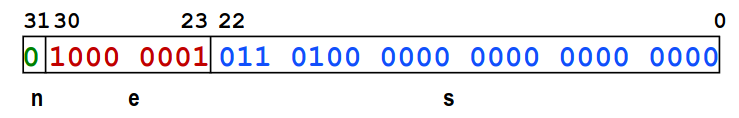
\includegraphics[scale=0.5]{img/float_encoding.png}
    \end{center}
    Doubles encode 64 bits, so not we have exponent having 11 bits (so bias is not 1023) and 52 bits for mantissa. 
  \end{theorem}

\section{Memory} 

    \begin{definition}[Memory]
      The \textbf{memory} is where the computer stores data and instructions, which can be though of as a giant array of memory addresses, with each containing a byte. This data consists of graphical things or even instructions to manipulate other data. It can be visualized  as a long array of boxes that each have an \textbf{address} (where it is located) and \textbf{contents} (what is stored in it).

      Memory simply works as a bunch of bits in your computer with each bit having some memory address, which is also a bit. For example, the memory address \texttt{0b0010} (2) may have the bit value of \texttt{0b1} (1) stored in it. 

      \begin{figure}[H]
        \centering 
        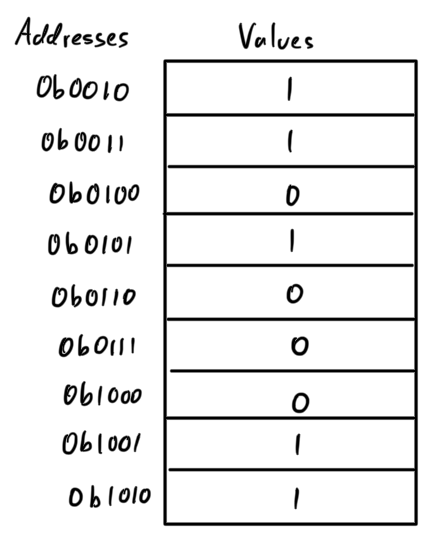
\includegraphics[scale=0.4]{img/memory_visual_bit.png}
        \caption{Visualization of memory as a long array of boxes of bits. }
        \label{fig:memory_visual_bit}
      \end{figure}

      However, computers do not need this fine grained level of control on the memory, and they really work at the Byte level rather than the bit level. Therefore, we can visualize the memory as a long array of boxes indexed by \textit{Bytes}, with each value being a byte as well. In short, the memory is \textbf{byte-addressable}. In certain arthitectures, some systems are \textbf{word-addressable}, meaning that the memory is addressed by words, which are 4 bytes.\footnote{Note that in here the size of a word is 2 bytes rather than 4 as stated above. This is just how it is defined in some \texttt{x86} architectures.}

      \begin{figure}[H]
        \centering 
        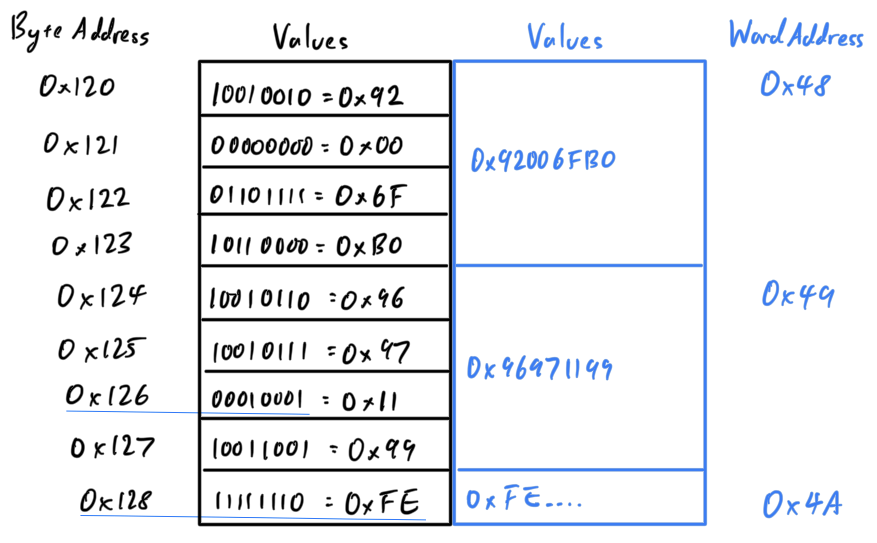
\includegraphics[scale=0.4]{img/memory_visual_byte.png}
        \caption{Visualization of memory as a long array of boxes of bytes. Every address is a byte and its corresponding value at that address is also a byte, though we represent it as a 2-digit hex. } 
        \label{fig:memory_visual_byte}
      \end{figure}
    \end{definition}

    In the examples above, I listed the memory addresses as a 3 hex character (1.5 bytes) for brevity. In reality, the number of bytes that a memory address takes is much longer. 

    \begin{definition}[32 and 64 Bit Machines]
      There are two types of machines that tend to format these boxes very differently: 32-bit and 64-bit machines. 
      \begin{enumerate}
        \item 32 bit machines store addresses in 32 bits, so they can have $2^{32}$ addresses, which is about 4 GB of memory. 
        \item 64 bit machines store addresses in 64 bits, so they can have $2^{64}$ addresses, which is about 16 EB of memory. This does not mean that the actual RAM is 16 EB, but it means that the machine can \textit{handle} that much memory. 
        \begin{lstlisting} 
          ...
          0x00007FFF7FBFF860 --> 0b000000000000000000000000011111111111
                                 111101111111101111111111100001100000
          0x00007FFF7FBFF861 --> 0b000000000000000000000000011111111111
                                 111101111111101111111111100001100001
          0x00007FFF7FBFF862 --> 0b000000000000000000000000011111111111
                                 111101111111101111111111100001100010
          0x00007FFF7FBFF863 --> 0b000000000000000000000000011111111111
                                 111101111111101111111111100001100011
          0x00007FFF7FBFF864 --> 0b000000000000000000000000011111111111
                                 111101111111101111111111100001100100
          ...
        \end{lstlisting}
      \end{enumerate}
      The numbers typically mean the size of the type that the machine works best with, so all memory addresses will be 32 or 64 bits wide. Most machines are 64-bits, and so everything in this notes will assume that we are working with a 64 bit machine. As we will later see, this is why pointers are 8 bytes long, i.e. 64 bits. This is because the memory addresses are 64 bits long, though all of them are not used. 
    \end{definition}

    With this structure in mind and knowing the size of some primitive types, we can now focus on how declaring them works in the backend. 

    \begin{definition}[Declaration, Initialization]
      Assigning a value to a variable is a two step process, which is often not distinguished in high level languages like Python. 
      \begin{enumerate}
        \item You must first \textbf{initialize} the variable by setting aside the correct number of bytes in memory. 
        \item You must then \textbf{assign} that variable to be some actual value. 
      \end{enumerate}
      The two step process is often called declaration. 
    \end{definition}

    This is the reason why C is statically, or strongly, typed. In order to set aside some memory for a variable, you must know how big that variable will be, which you know by its type. This makes sense. We can first demonstrate how to both initialize and declare a variable. 

    \begin{figure}[H]
      \centering 
      \noindent\begin{minipage}{.5\textwidth}
      \begin{lstlisting}[]{Code}
        int main() {
          // declaring 
          int x = 4;   
          printf("%p\n", &x); 
          
          // initializing and assigning
          int y; 
          printf("%p\n", &y); 
          y = 3; 
          printf("%p\n", &y); 

          return 0; 
        }
      \end{lstlisting}
      \end{minipage}
      \hfill
      \begin{minipage}{.49\textwidth}
      \begin{lstlisting}[]{Output}
        0x16d37ee68
        0x16d37ee64
        0x16d37ee64 
        .
        .
        .
        .
        .
        .
        .
        .
        .
        .
      \end{lstlisting}
      \end{minipage}
      \caption{How to declare variables in C. As you can see, by initializing \texttt{y}, the memory address is already assigned and it doesn't change when you assign it. The address is only shown to be 9 hex digits long, but it is actually 16 hex digits long and simply 0 padded on the left. } 
      \label{fig:declaring_initializing_variables}
    \end{figure}

    One question that may come to mind is, what is the value of the variable if you just initialize it? After all the value at that address that is initialized must be either $0$s or $1$s. Let's find out. 

    \begin{figure}[H]
      \centering 
      \noindent\begin{minipage}{.5\textwidth}
      \begin{lstlisting}[]{Code}
        int main() { 
          int y; 
          printf("%d\n", y); 
          y = 3; 
          printf("%d\n", y); 

          return 0; 
        }
      \end{lstlisting}
      \end{minipage}
      \hfill
      \begin{minipage}{.49\textwidth}
      \begin{lstlisting}[]{Output}
        6298576 
        3
        .
        .
        .
        .
        .
        .
      \end{lstlisting}
      \end{minipage}
      \caption{The value of an uninitialized variable is some random number. } 
      \label{fig:uninitialized_variable}
    \end{figure}

    It may be interesting to see how this random unititialized value is generated. It is simply the value that was stored in that memory address before, and it is not cleared when you initialize it, so you should not use this as a uniform random number generator. 

  \subsection{Debugging and Object Dumping} 

    Talk about gdb, lldb, objdump, etc. These are debugging tools that allow you to parse your code line by line. However, to actually see the C code, you must compile it with the debugging flag. This adds a little bit of overhead memory to the binary, but not a lot. 

  \subsection{Endian Architecture}

    It is intuitive to think that given some multi-byte object like an \texttt{int} (4 bytes), the beginning of the int would be the lowest address and the end of the int would be the highest address, like how consecutive integers are stored in an array. However, this is not always the case (almost always not the case since most computers are little-endian).  

    \begin{definition}[Endian Architecture]
      Depending on the machine architecture, computers may store these types slightly differently in their \textit{byte} order. Say that we have an integer of value \texttt{0xA1B2C3D4} (4 bytes). Then, 
      \begin{enumerate} 
        \item A \textbf{big-endian architecture} (e.g. SPARC, z/Architecture) will store it so that the least significant byte has the highest address.
        \item A \textbf{little-endian architecture} (e.g. x86, x86-64, RISC-V) will store it so that the least significant byte has the lowest address. 
        \item A \textbf{bi-endian architecture} (e.g. ARM, PowerPC) can specify the endianness as big or little. 
      \end{enumerate}

      \begin{figure}[H]
        \centering 
        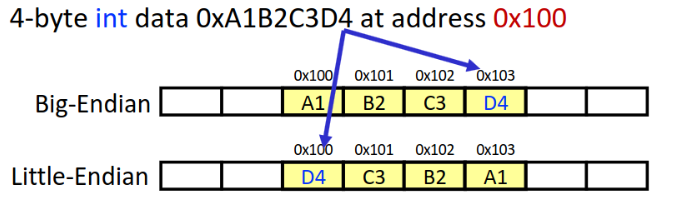
\includegraphics[scale=0.4]{img/endianness.png}
        \caption{The big vs little endian architectures. } 
        \label{fig:endianness}
      \end{figure}
    \end{definition}

    We can simply print out the hex values of primitive types to see how they are stored in memory, but it does not provide the level of details that we want on which bytes are stored where. At this point, we must use certain \textbf{debuggers} to directly look at the memory. For x86 architectures, we can use \texttt{gdb} and for ARM architectures, we can use \texttt{lldb}. At this point, we need to understand assembly to look through debuggers, so we will provide the example here. 

    \begin{example}[Endianness of C Int in x86-64]
      To do. 
    \end{example}

    \begin{example}[Endianness of C Int in ARM64]
      To do. 
    \end{example}

  \subsection{Type Casting}


  \subsection{Pointers}

    We have learned how to declare/initialize a variable, which frees up some space in the memory and possibly assigns a value to it. One great trait of C is that we can also store the memory address of a variable in another variable called a pointer. You access both the memory and the value at that memory with this pointer variable. 

    \begin{definition}[Pointer Variable]
      A \textbf{pointer} variable/type is a variable that stores the memory address of another variable. 
      \begin{enumerate}
        \item You can declare a pointer in the same way that you declare a variable, but you must add a asterisk in front of the variable name. 
        \item The size of this variable is the size of the memory address, which is 8 bytes in a 64-bit architecture. 
        \item To get the value of the variable that the pointer points to, called \textbf{dereferencing}, you simply put a asterisk in front of the pointer. This is similar to how you put a ampersand in front of a variable to get its memory address. 
      \end{enumerate}

      \begin{figure}[H]
        \centering 
        \noindent\begin{minipage}{.5\textwidth}
        \begin{lstlisting}[]{Code}
          int main() { 
            // declare an integer 
            int x = 4; 
            printf("x = %d\n", x); 
            printf("&x = %p\n", &x); 

            // declare pointer 
            int *p = &x; 
            printf("p = %p\n", p); 
            printf("*p = %d\n", *p); 

            // initialize pointer 
            int *q; 
            q = &x; 
            printf("q = %p\n", q); 
            printf("*q = %d\n", *q); 
            return 0; 
          }
          
        \end{lstlisting}
        \end{minipage}
        \hfill
        \begin{minipage}{.49\textwidth}
        \begin{lstlisting}[]{Output}
          x = 4
          &x = 0x16d49ae68
          p = 0x16d49ae68
          *p = 4
          q = 0x16d49ae68
          *q = 4
          .
          .
          .
          .
          .
          .
          .
          .
          .
          .
          .
          .
        \end{lstlisting}
        \end{minipage}
        \caption{} 
        \label{fig:pointer_variable}
      \end{figure}
    \end{definition}

    Since the size of addresses are predetermined by the architecture, it may not seem like we need to know the underlying data type of what it points to, so why do we need to write strongly type the underlying data type? Remember that to do pointer arithmetic, you need to know how large the underlying data type is so that you can know how many bytes to move when traversing down an array. 

    One of the reasons why pointers are so valuable is that they allow you to pass by reference, which is a way to change the value of a variable in a function. 

    \subsubsection{Call by Value vs Call by Reference}

      \begin{definition}[Call by Value]
        
      \end{definition}

      \begin{definition}[Call by Reference]
        
      \end{definition}
    
    \subsubsection{Pointer Errors}

      Just like for regular variables, you may be curious on the value of an unassigned pointer. Let's take a look. 

      \begin{example}[Uninitialized Pointers]
      \begin{figure}[H]
        \centering 
        \noindent\begin{minipage}{.5\textwidth}
        \begin{lstlisting}[]{Code}
          int main() { 
            int x = 4; 
            int *p; 
            printf("p = %p\n", p); 
            printf("*p = %x\n", *p); 

            return 0; 
          }
        \end{lstlisting}
        \end{minipage}
        \hfill
        \begin{minipage}{.49\textwidth}
        \begin{lstlisting}[]{Output}
          p = 0x10249ff20
          *p = d100c3ff
          .
          .
          .
          .
          .
          .
        \end{lstlisting}
        \end{minipage}
        \caption{The value of an uninitialized pointer is some random address and at a random address it would be some random byte. } 
        \label{fig:uninitialized_pointer}
      \end{figure}
      \end{example}

      This is clearly not good, especially since the program compiles correctly and runs without any errors. This kind of pointer that hasn't been initialized is called a wild pointer. 

      \begin{definition}[Wild Pointer]
        A \textbf{wild pointer} is a pointer that has not been initialized to a known value. 
      \end{definition}

      To fix this, we must always initialize a pointer to a known value. This may come at a disadvantage, since now we can't reap the benefits of initializing first and assigning later. A nice compromise is to initialize the pointer to a null pointer. 

      \begin{definition}[Null Pointer]
        A \textbf{null pointer} is a pointer that has been initialized to a known value, which is the address 0x0. You can set the type of the pointer and then initialize it to \texttt{NULL}. 
      \begin{figure}[H]
        \centering 
        \noindent\begin{minipage}{.5\textwidth}
        \begin{lstlisting}[]{Code}
          int main() { 
            int *p = NULL; 
            printf("p = %p\n", p); 
            
            // the code below gives seg fault
            /* printf("*p = %d\n", *p); */

            int x = 4; 
            p = &x; 
            printf("p = %p\n", p); 
            printf("*p = %d\n", *p);
            return 0; 
          }
        \end{lstlisting}
        \end{minipage}
        \hfill
        \begin{minipage}{.49\textwidth}
        \begin{lstlisting}[]{Output}
          p = 0x0
          p = 0x16da72e5c
          *p = 4
          .
          .
          .
          .
          .
          .
          .
          .
          .
          .
        \end{lstlisting}
        \end{minipage}
        \caption{Initializing a null pointer. It is a good practice to initialize a pointer to a null value. } 
        \label{fig:null_pointer}
      \end{figure}
      \end{definition}

      Therefore, the null pointer allows you to set the type of the underlying data type, but the actual address will be 0x0. You cannot dereference a null pointer, and doing so will give you a segmentation fault. There may be times when you do not even know the data type of the pointer, and for this you can use the void pointer, which now doesn't know the type of the variable that it points to but it does allocate address. 

      \begin{definition}[Void Pointer]
        A \textbf{void pointer} is a pointer that does not know the type of the variable that it points to. We can initialize it by simply setting the underlying type to be void. This initializes the address, which should always be 8 bytes, but trying to access the value of the variable is not possible. 
        \begin{figure}[H]
          \centering 
          \noindent\begin{minipage}{.5\textwidth}
          \begin{lstlisting}[]{Code}
            int main() { 
              void *p; 
              printf("p = %p\n", p); 
              int x = 4; 
              p = &x; 
              printf("%d", *((int*)p));
              return 0; 
            }
          \end{lstlisting}
          \end{minipage}
          \hfill
          \begin{minipage}{.49\textwidth}
          \begin{lstlisting}[]{Output}
            p = 0x102553f54
            4 
            .
            .
            .
            .
            .
            .
          \end{lstlisting}
          \end{minipage}
          \caption{Initialize a void pointer and then use typecasting to access the value of the variable that it points to. } 
          \label{fig:initialize_void_pointer}
        \end{figure}
      \end{definition}

  \subsection{Pointer Arithmetic} 

    With pointers out of the way, we can talk about how arrays are stored in memory. 

    \begin{definition}[Array]
      A C array is a collection of elements of the same type, which are stored in contiguous memory locations. You can initialize and declare arrays in many ways, and access their elements with the index, e.g. \texttt{arr[i]}.
      \begin{enumerate}
        \item You declare an array of some constant number of elements $n$ with the elements themselves. 
          \begin{lstlisting} 
            int arr[5] = {1, 2, 3, 4, 5}; 
          \end{lstlisting}
        \item You declare an array with out its size $n$ and simply assign them. Then $n$ is automatically determined. 
          \begin{lstlisting} 
            int arr[] = {1, 2, 3, 4, 5}; 
          \end{lstlisting}
        \item You initialize an array of some constant size $c$, and then you assign each element of the array. 
          \begin{lstlisting} 
            int arr[5]; 
            for (int i = 0; i < 5; i++) {
              arr[i] = i + 1; 
            }
          \end{lstlisting}
      \end{enumerate}
      Unfortunately, C does not provide a built-in way to get the size of the array (like \texttt{len} in Python), so we must keep track of the size of the array ourselves. Furthermore, the address of the array is the address of where it begins at, i.e. the address of the first element. 
    \end{definition}

    You can literally see that the elements of the array are contiguous in memory by iterating through each element and printing out its address. 

    \begin{figure}[H]
      \centering 
      \noindent\begin{minipage}{.5\textwidth}
      \begin{lstlisting}[]{Code}
        int main(void) {
          // initialize array 
          int arr[5]; 
          for (int val = 1; val < 6; val++) {
            arr[val-1] = val * val;
          }

          int* p = &arr[0]; 
          for (int i = 0; i < 5; i++) {
            printf("Value at position %d : %d\n", i, arr[i]); 
            printf("Address at position %d : %p\n", i, p + i); 
          }

          return 0; 
        }        
      \end{lstlisting}
      \end{minipage}
      \hfill
      \begin{minipage}{.49\textwidth}
      \begin{lstlisting}[]{Output}
        Value at position 0 : 1
        Address at position 0 : 0x7ffd8636b0d0
        Value at position 1 : 4
        Address at position 1 : 0x7ffd8636b0d4
        Value at position 2 : 9
        Address at position 2 : 0x7ffd8636b0d8
        Value at position 3 : 16
        Address at position 3 : 0x7ffd8636b0dc
        Value at position 4 : 25
        Address at position 4 : 0x7ffd8636b0e0
        .
        .
        .
        .
        .
        .
        .
      \end{lstlisting}
      \end{minipage}
      \caption{Ints are 4 bytes long, so the address of the next element is 4 bytes away from the previous element, making this a contiguous array.} 
      \label{fig:contiguous_array}
    \end{figure}

    The most familiar implementation of an array is a string in C. 

    \begin{definition}[String]
      A string is an array of characters, which is terminated by a null character \texttt{\textbackslash 0}. You can initialize them in two ways: 
      \begin{enumerate}
        \item You can declare a string with the characters themselves, which you must make sure to end with the null character. 
          \begin{lstlisting} 
            char str[6] = {'H', 'e', 'l', 'l', 'o', '\0'}; 
          \end{lstlisting}
        \item You can declare them with double quotes, which automatically adds the null character. 
          \begin{lstlisting} 
            char str[] = "Hello"; 
          \end{lstlisting}
      \end{enumerate}
      Note that for whatever string we initialize, the size of the array is the number of characters plus 1. 
    \end{definition}

    To access elements of an array, you simply use the index of the element, e.g. \texttt{arr[i]}, but in the backend, this is implemented with \textit{pointer arithmetic}. 

    \begin{definition}[Pointer Arithmetic]
      Pointer arithmetic is the arithmetic of pointers, which is done by adding or subtracting an integer to a pointer. 
      \begin{enumerate}
        \item If you add an integer $n$ to a pointer $p$, e.g. \texttt{p + n}, then the new pointer will point to the $n$th element after the current element, with the next element being \texttt{sizeof(type)} bytes away from the pervious element. 
        \item If you subtract an integer $n$ from a pointer, then the pointer will point to the $n$th element before the current element. 
      \end{enumerate}
      This is why you can access the elements of an array with the index, since the index is simply the number of elements away from the first element.
    \end{definition}

    \begin{example}[Pointer Arithmetic with Arrays of Ints and Chars]
      Ints have a size of 4 bytes and chars 1 byte. You can see that using pointer arithmetic, the addresses of the elements of ints increment by 4 and those of the char array increment by 1. 
      \noindent\begin{minipage}{.5\textwidth}
      \begin{lstlisting}[]{Code}
        int main() { 
          int integers[3] = {1, 2, 3}; 
          char characters[3] = {'a', 'b', 'c'};
          int *p = &integers[0]; 
          char *q = &characters[0];
          
          printf("Array of Integers\n"); 
          for (int i = 0; i < 3; i++) { 
            printf("%p\n", integers+i); }

          printf("Array of Characters\n"); 
          for (int i = 0; i < 3; i++) { 
            printf("%p\n", characters+i); }
          return 0; 
        }
      \end{lstlisting}
      \end{minipage}
      \hfill
      \begin{minipage}{.49\textwidth}
      \begin{lstlisting}[]{Output}
        Array of Integers
        0x16d39ee58
        0x16d39ee5c
        0x16d39ee60
        .
        Array of Characters
        0x16d39ee50
        0x16d39ee51
        0x16d39ee52
        .
        .
        .
        .
        .
        .
      \end{lstlisting}
      \end{minipage}
    \end{example}

    Therefore, we can think of accessing the elements of an array as simply pointer arithmetic. 

    \begin{theorem}[Bracket Notation is Pointer Arithmetic]
      The bracket notation is simply pointer arithmetic in the backend. 
      \begin{figure}[H]
        \centering 
        \noindent\begin{minipage}{.5\textwidth}
        \begin{lstlisting}[]{Code}
          int main() { 
            int arr[3] = {1, 2, 3}; 
            int *p = &arr[0]; 

            for (int i = 0; i < 3; i++) { 
              printf("%d\n", arr[i]); 
              printf("%d\n", *(p+i)); 
            }
            return 0; 
          }
        \end{lstlisting}
        \end{minipage}
        \hfill
        \begin{minipage}{.49\textwidth}
        \begin{lstlisting}[]{Output}
          1
          1
          2
          2
          3
          3
          .
          .
          .
          .
        \end{lstlisting}
        \end{minipage}
        \caption{Accessing the elements of the list using both ways is indeed the same. } 
        \label{fig:bracket_pointer_arthimetic}
      \end{figure}
    \end{theorem}
   
  \subsection{Global, Stack, and Heap Memory}

    Everything in a program is stored in memory, variables, functions, and even the code itself. However, we will find out that they are stored in different parts of the memory. When a program runs, its application memory consists of four parts, as visualized in the Figure \ref{fig:memory_layout}. 
    \begin{enumerate} 
      \item The \textbf{code} is where the code text is stored. 
      \item The \textbf{global memory} is where all the global variables are stored. 
      \item The \textbf{stack} is where all of the functions and local variables are stored. 
      \item The \textbf{heap} is variable and can expand to as much as the RAM on the current system. We can specifically store whatever variables we want in the heap.
    \end{enumerate}

    We provide a visual of these four parts first, and we will go into them later. 
    \begin{figure}[H]
      \centering 
      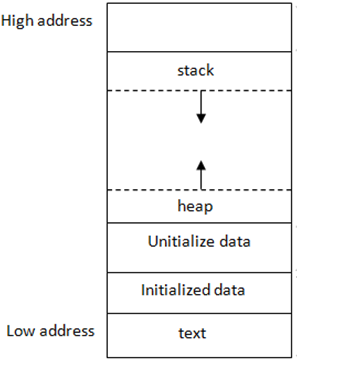
\includegraphics[scale=0.6]{img/memory_layout.png}
      \caption{The four parts of memory in a C program.} 
      \label{fig:memory_layout} 
    \end{figure}

    \begin{definition}[Code Memory]
      This is where the code text is stored. It is read-only and is not modifiable.
    \end{definition}

    In high level languages, we always talk about local and global scope. That is, variables defined within functions have a local scope in the sense that anything we modify in the local scope does not affect the global scope. We can now understand what this actually means by examining the backend.  The global scope variables are stored in the global memory, and all local variables (and functions) are stored in the stack. 


    \begin{definition}[Global Memory]
      This is where all the global variables are stored. 
    \end{definition}

    \begin{definition}[Stack Memory]
      This is where all of the functions and local variables are stored. As we will see later, the compiler will always run the main function, which must exist in your file. By the main function is a function itself, and therefore it has its own local scope. 

      Then, when you initialize any functions or local variables within those functions (which will be the majority of your code), all these will be stored in the stack, which is an literally an implementation of the stack data structure. It is LIFO, and the first thing that goes in is the \texttt{main} function and its local variables, which is referred to as the \textbf{stack frame}. You can't free memory in the stack unless its in the top of the stack. 
    \end{definition}

    To see what happens in the stack, we can go through an example. 

    \begin{example}[Going through the Stack]
      Say that you have the following code: 

      \begin{lstlisting} 
        int total; 
        int Square(int x) {
          return x*x; 
        }
        int SquareOfSum(int x, int y) {
          int z = Square(x + y); 
          return z; 
        }
        int main() { 
          int a = 4, b = 8;              
          total = SquareOfSum(a, b); 
          printf("output = %d", total); 
          return 0; 
        }
      \end{lstlisting}
      
      The memory allocation of this program will run as such: 
      \begin{enumerate} 
        \item The \texttt{total} variable is initialized and is put into global memory. 
        \item \texttt{main} is called. It is put into the stack. 
        \item The local variables \texttt{a=4} and \texttt{b=8} are initialized and are put into the stack. 
        \item The \texttt{SquareOfSum} function is called and put into the stack. 
        \item The input local variables \texttt{x=4}, \texttt{y=8}, \texttt{z} are initialized and put into the stack. 
        \item \texttt{x + y=12} is computed and put into the stack. 
        \item The \texttt{Square} function is called and put into the stack. 
        \item The \texttt{x=12} local variable of \texttt{Square} is initialized and put into the stack. 
        \item The CPU computes \texttt{x*x=144} and returns the output. The \texttt{Square} function is removed from the stack. 
        \item We assign \texttt{z=144} and \texttt{SquareOfSum} returns it. Now \texttt{SquareOfSum} is removed from the stack. 
        \item \texttt{total=144} is assigned in the global memory still. 
        \item The \texttt{printf} function is called and put into the stack. 
        \item The \texttt{printf} function prints the output and is removed from the stack. 
        \item The \texttt{main} function returns \texttt{0} and is removed from the stack, ending our application. 
      \end{enumerate}
    \end{example}


    One limitation of the stack is that its total available memory is fixed from the start, ranging from 1MB to 8MB, and so you can't initialize arrays of billions of integers in the stack. It will cause a memory overflow. In fact, the memory of the stack, along with the global and text memory, are assigned at compile time, making it a \textbf{static memory}. 

    Since the stack is really just a very small portion of available memory, the heap comes into rescue, which is the pool of memory available to you in RAM. 

    \begin{definition}[Heap Memory]
      The \textbf{heap memory} (nothing to do with the heap data structure) is a variable length (meaning it can grow at runtime) and \textbf{dynamically allocated} (meaning that we can assign memory addresses during runtime) memory that is limited to your computer's hardware. Unlike simply initializing variables to allocate memory as in the stack, we must use the \textbf{malloc} and \textbf{free} functions in C, and \textbf{new} and \textbf{delete} operations in C++. 
    \end{definition}

    \begin{definition}[malloc]
      
    \end{definition}

    \begin{definition}[free]
      
    \end{definition}

    The stack can store pointer variables that point to the memory address in the heap. So the only way to access variables in the heap is through pointer reference, and the stack provides you that window to access that big pool of heap memory. 


    One warning: if you allocate another address, the previous address does not get deallocated off the memory. 

    \begin{definition}[Memory Leak]
      
    \end{definition}

    On the other hand, if you free an address but have a pointer still pointing to that address, this is also a problem called the dangling pointer. 

    \begin{definition}[Dangling Pointer]
      
    \end{definition}

    At this point, we might be wondering why we need both a stack and a heap. Well the benefits of heaps are clearer since you can dynamically allocate memory, and you don't have the LIFO paradigm that is blocking you from deallocating memory that has been allocated in the beginning of your program. A problem with just having heap is that stacks can be orders of magnitude times faster when allocating/deallocating from it than the heap, and the sequence of function calls is naturally represented as a stack. 

  \subsection{Dynamic Memory Allocation}

    Let's talk about how \texttt{malloc} and \texttt{free} are implemented in C. If you make a for loop and simply print all the addresses that you allocate to. You will find that they can be quite random. After a program makes some calls to malloc and free, the heap memory can becomes fragmented, meaning that there are chunks of free heap space interspersed with chunks of allocated heap space. The heap memory manager typically keeps lists of different ranges of sizes of heap space to enable fast searching for a free extent of a particular size. In addition, it implements one or more policies for choosing among multiple free extents that could be used to satisfy a request.

    The free function may seem odd in that it only expects to receive the address of the heap space to free without needing the size of the heap space to free at that address. That’s because malloc not only allocates the requested memory bytes, but it also allocates a few additional bytes right before the allocated chunk to store a header structure. The header stores metadata about the allocated chunk of heap space, such as the size. As a result, a call to free only needs to pass the address of heap memory to free. The implementation of free can get the size of the memory to free from the header information that is in memory right before the address passed to free.

\section{Implementations of Memory Structures in C} 

  \subsection{Arrays}

  \subsection{Strings}

  \subsection{Structs}

  \subsection{Functions}

  \subsection{Classes (for C++)}

  \subsection{Input Output}
    
    We have standard in, standard out, and standard error. 

\section{Central Processing Unit} 

    Now let's talk about how functions work on a deeper level. When we write a command, like \texttt{int x = 4}, we are manually looking for an address (in the stack, global, or heap) and rewriting the bits that are at that address. Functions are just an automated way to do this, and all these modifications and computations are done by the CPU. 

    \begin{definition}[Central Processing Unit]
      The CPU is responsible for taking instructions (data) from memory and executing them. 
      \begin{enumerate} 
        \item The CPU is composed of \textbf{registers} (different from the cache), which are small, fast storage locations. These registers can either be \textbf{general purpose} (can be used with most instructions) or \textbf{special purpose} (can be accessed through special instructions, or have special meanings/uses, or are simply faster when used in a specific way).
        \item The CPU also has an \textbf{arithmetic unit} and \textbf{logic unit}, which is responsible for performing arithmetic and logical operations. 
        \item The CPU also has a \textbf{control unit}, which is responsible for fetching instructions from memory through the \textbf{databus}, which is literally a wire connecting the CPU and RAM, and executing them. 
      \end{enumerate}
      It executes instructions from memory one at a time and executes them, known as the \textbf{fetch-execute cycle}. It consists of 4 main operations. 
      \begin{enumerate} 
        \item \textbf{Fetch}: The \textbf{program counter}, which holds the memory address of the next instruction to be executed, tells the control unit to fetch the instruction from memory through the databus. 
        \item \textbf{Decode}: The fetched data is passed to the \textbf{instruction decoder}, which figures out what the instruction is and what it does and stores them in the registers.
        \item \textbf{Execute}: The arithmetic and logic unit then carries out these operations. 
        \item \textbf{Store}: Then it puts the results back on the databus, and stores them back into memory.
      \end{enumerate} 
      The CPU's \textbf{clock cycle} is the time it takes for the CPU to execute one instruction. More specifically, the clock cycle refers to a single oscillation of the clock signal that synchronizes the operations of the processor and the memory (e.g. fetch, decode, execute, store), and decent computers have clock cycles of at least $2.60$GHz (2.6 billion clock cycles per second). 
    \end{definition}

    Therefore, in order to actually do computations on the data stored in the memory, the CPU must first fetch the data, perform the computations, and then store the results back into memory. This can be done in two ways.

    \begin{enumerate}
      \item Load and Store Operations: CPUs use load instructions to move data from memory to registers (where operations can be performed more quickly) and store instructions to move the modified data back into memory.
      \item If the data is too big to fit into the registers, the CPU will use the \textbf{cache} to store the data, and in worse cases, the actual memory itself. Compilers optimize code by maximizing the use of registers for operations to minimize slow memory access. This is why you often see assembly code doing a lot in registers.
    \end{enumerate}

    To clarify, let us compare registers and memory. Memory is addressed by an unsigned integer while registers have names like \texttt{\%rsi}. Memory is much bigger at several GB, while the total register space is much smaller at around 128 bytes (may differ depending on the architecture). The memory is much slower than registers, which is usually on a sub-nanosecond timescale. The memory is dynamic and can grow as needed while the registers are static and cannot grow.

    The specific structure/architecture of the CPU is determined by the instruction set architecture (ISA), which can be thought of as a subset of the general computer architecture. 

    \begin{definition}[Instruction Set Architecture]
      The \textbf{ISA} or just \textbf{architecture} of a CPU is a high level description of what it can do. Some differences are listed here: 
      \begin{enumerate} 
        \item What instructions it can execute. 
        \item The instruction length and decoding, along with its complexity. 
        \item The performance vs power efficiency. 
      \end{enumerate}
      ISAs can be classified into two types. 
      \begin{enumerate} 
        \item The \textbf{complex instruction set computer} (CISC) is characterized by a large set of complex instructions, which can execute a variety of low-level operations. This approach aims to reduce the number of instructions per program, attempting to achieve higher efficiency by performing more operations with fewer instructions.
        \item The \textbf{reduced instruction set computer} (RISC) emphasizes simplicity and efficiency with a smaller number of instructions that are generally simpler and more uniform in size and format. This approach facilitates faster instruction execution and easier pipelining, with the philosophy that simpler instructions can provide greater performance when optimized.
      \end{enumerate}
    \end{definition}

    Just like how memory addressing is different between 32 and 64 bit machines, CPUs also use these schemes. While 32-bit processors have $2^{32}$ possible addresses in their cache, it turns out that 64-bit processors have a 48-address space. This is because CPU manufacturers took a shortcut. They use an instruction set which allows a full 64-bit address space, but current CPUs just only use the last 48-bits. The alternative was wasting transistors on handling a bigger address space which wasn't going to be needed for many years (since 48-bits is about 256TB). Just a bit of history for you. Finally, just to briefly mention, the input/output device, as the name suggests, processes inputs and displays outputs, which is how you can see what the program does. 

    \begin{example}[x86 Architecture]
      The x86 architecture is a CISC architecture, which is the most common architecture for personal computers. Here are important properties: 
      \begin{enumerate} 
        \item It is a complex instruction set computer (CISC) architecture, which means that it has a large set of complex instructions\footnote{https://en.wikipedia.org/wiki/X86\_instruction\_listings}. 
        \item Byte-addressing is enabled and words are stored in little-endian format.
        \item In the x86\_64 architecture, registers are 8 bytes long (and 4 bytes in x86\_32) and there are 16 total general purpose registers, for a total of only 128 bytes (very small compared to many GB of memory). Other special purpose registers are also documented in the wikipedia page, but it is not fully documented. 
      \end{enumerate}
    \end{example}

    \begin{example}[ARM Archiecture]
      Mainly in phones, tablets, laptops. 
    \end{example}

    \begin{example}[MIPS Architecture]
      MIPS is a RISC architecture, which is used in embedded systems such as digital home and networking equipment. 
    \end{example}


    \begin{definition}[Input/Output Device]
      The input device can read/load/write/store data from the outside world. The output device, which has \textbf{direct memory address}, can display data to the outside world. 
    \end{definition}

    One final note to mention, there are many assembly languages out there and various syntaxes. 

    \begin{example}[Assembly Syntax]
      The two most popular syntaxes are AT\&T and Intel. 
      \begin{enumerate}
        \item \textbf{Intel Syntax}: Specifies memory operands without any special prefixes. Square brackets [] are used to denote memory addresses. For example, mov eax, [ebx] means move the contents of the memory location pointed to by ebx into eax.

        \item \textbf{AT\&T Syntax}: Memory operands are denoted with parentheses () and include the \% prefix for registers. An instruction moving data from a memory location into a register might look like movl (\%ebx), \%eax, with additional prefixes for immediate values and segment overrides.
      \end{enumerate}
    \end{example}

    \begin{example}[Assembly Languages]
      The various assembly languages are as follows: 
      \begin{enumerate}
        \item \textbf{x86 Assembly} : The assembly language for Intel and AMD processors using the x86 architecture. Both AT\&T and Intel syntax are available. Tools or environments often allow switching between the two, with AT\&T being the default in GNU tools like GDB.
        
        \item \textbf{ARM Assembly} : The assembly language for ARM processors. Has its own unique syntax, not categorized as AT\&T or Intel. ARM syntax is closely tied to its instruction set architecture and is distinct from the x86 conventions.
        
        \item \textbf{MIPS Assembly} : The assembly language for MIPS processors. MIPS uses its own assembly language syntax, which is neither AT\&T nor Intel. MIPS syntax is designed around the MIPS instruction set architecture.
        
        \item \textbf{PowerPC Assembly} : The assembly language for PowerPC processors. PowerPC has its own syntax style, tailored to its architecture and instruction set, distinct from the AT\&T and Intel syntax models.
        
        \item \textbf{6502 Assembly} : Used in many early microcomputers and gaming consoles. Utilizes a syntax unique to the 6502 processor, not following AT\&T or Intel conventions.
        
        \item \textbf{AVR Assembly} : The assembly language for Atmel's AVR microcontrollers. AVR assembly follows its own syntax style, designed specifically for AVR microcontrollers and not based on AT\&T or Intel syntax.
        
        \item \textbf{Z80 Assembly} : Associated with the Z80 microprocessor, used in numerous computing devices in the late 20th century. Z80 assembly language has its own syntax that does not adhere to AT\&T or Intel syntax guidelines.
      \end{enumerate}
    \end{example}

    The most common one is the x86\_64, which is the one that we will be focusing on, with the AT\%T syntax. 

  \subsection{Circuits} 

    Let's go over some common logic gates since this is at the basis of how to construct arithmetic operations. 
    
    \begin{definition}[AND, NOT, OR]
      
    \end{definition}

    \begin{definition}[XOR, NAND, NOR]
      
    \end{definition}

    \begin{definition}[NAND]
      
    \end{definition}

    Talk about how to construct arithmetic operations with these gates such as adding two integers or multiplying them, and not just that, but other operations that we may need in a programming language. 

    \begin{theorem}[Implementation of Moving Data in Circuits]
      
    \end{theorem}

    \begin{theorem}[Implementation of Addition, Subtraction in Circuits]
      
    \end{theorem}

    \begin{theorem}[Implementation of Multiplication in Circuits]
      
    \end{theorem}

    \begin{theorem}[Implementation of Bitwise Operations in Circuits]
      
    \end{theorem}

    \begin{theorem}[Implementation of Bitshift Operations]
      
    \end{theorem}

    We also want some sort of conditionals. This then can be used to implement loops by checking some conditional. 

    \begin{theorem}[Implementation of Conditionals in Circuits]
      
    \end{theorem}

    As a bonus, we talk about the difference between volatile and non-volatile memory. We already learned that RAM is volatile, and this is simple to implement in a circuit since we can manually set all the bits to $0$ or just deplete all power. If this is the case, then how does non-volatile memory like SSDs maintain their state? 

    \begin{theorem}[Implementation of Volatile Memory]
      
    \end{theorem}

    \begin{theorem}[Implementation of Non-Volatile Memory]
      
    \end{theorem}

  \subsection{Registers}

      To understand anything that the CPU does, we must understand assembly language. In here, everything is done within registers, and we can see how the CPU fetches, decodes, and executes instructions. So what exactly are these registers? 

      \begin{definition}[Register]
        A register is a small, fast storage location within the CPU. It is used to store data that is being used immediately, and is the only place where the CPU can perform operations, which is why it must move data from memory to registers before it can perform operations on it. Everything in a register is in binary, at most 8 bytes, or 64 bits. 

        There are very specific types of registers that you should know. All of these registers are implemented for all assembly languages and are integral to the workflow of the CPU.  
        \begin{enumerate}
          \item \textbf{parameter registers} which store the parameters of a function.
          \item \textbf{Return registers} which store return values of functions. 
          \item \textbf{stack pointers} which point to the top of the stack (at the top of the current stack frame). 
          \item \textbf{frame pointers} which point to the base of the current stack frame.
          \item \textbf{instruction pointers} which point to the next instruction to be executed.
        \end{enumerate}
      \end{definition}

    \subsubsection{x86 Assembly Registers}

      The specific type of registers that are available to a CPU depends on the computer architecture, or more specifically, the ISA, but here is a list of common ones for the x86-64. We have \texttt{\%rax}, \texttt{\%rbx}, \texttt{\%rcx}, \texttt{\%rdx}, \texttt{\%rsi}, \texttt{\%rdi}, \texttt{\%rbp}, \texttt{\%rsp}, \texttt{\%r8}, \texttt{\%r9}, \texttt{\%r10}, \texttt{\%r11}, \texttt{\%r12}, \texttt{\%r13}, \texttt{\%r14}, \texttt{\%r15}. Therefore, the x86-64 Intel CPU has a total of 16 registers for storing 64 bit data. However, it is important to know which registers are used for what. 

      \begin{definition}[Parameter Registers]
        Compilers typically store the first six parameters of a function in registers 
        \begin{equation}
          \texttt{\%rdi}, \texttt{\%rsi}, \texttt{\%rdx}, \texttt{\%rcx}, \texttt{\%r8}, \texttt{\%r9}, 
        \end{equation}
        respectively. 
      \end{definition}

      \begin{definition}[Return Register]
        The return value of a function is stored in the 
        \begin{equation}
          \texttt{\%rax} 
        \end{equation}
        register.
      \end{definition}

      \begin{definition}[Stack and Frame Pointers]
        The \texttt{\%rsp} register is the \textbf{stack pointer}, which points to the top of the stack. The \texttt{\%rbp} register is the \textbf{frame pointer}, or \textbf{base pointer}, which points to the base of the current stack frame. In a typical function prologue, \textbf{\%rbp} is set to the current stack pointer (\textbf{\%rsp}) value, and then \texttt{\%rsp} is adjusted to allocate space for the local variables of the function. This establishes a fixed point of reference (\texttt{\%rbp}) for accessing those variables and parameters, even as the stack pointer (\texttt{\%rbp}) moves.
      \end{definition}

      \begin{definition}[Instruction Pointer]
        The \texttt{\%rip} register is the \textbf{instruction pointer}, which points to the next instruction to be executed. Unlike all the registers that we have shown so far, programs cannot write directly to \texttt{\%rip}. 
      \end{definition}


      \begin{definition}[Notation for Accessing Lower Bytes of Registers]
        Sometimes, we need a more fine grained control of these registers, and x86-64 provides a way to access the lower bits of the 64 bit registers. We can visualize them with the diagram below. 
        \begin{figure}[H]
          \centering 
          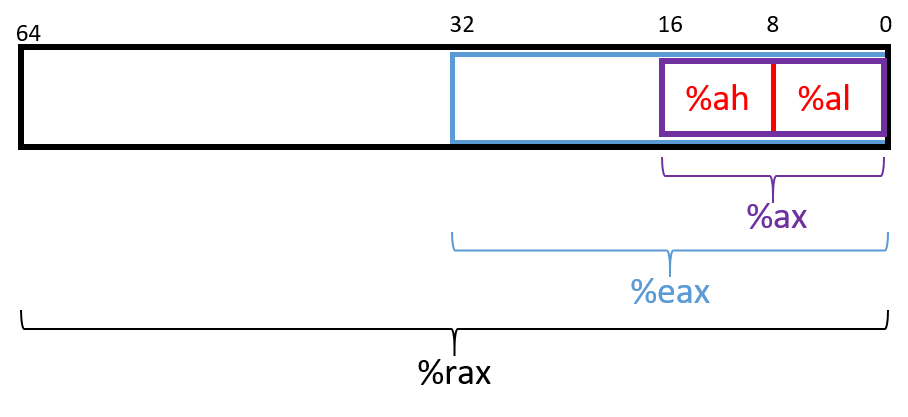
\includegraphics[scale=0.6]{img/register_subsets.png}
          \caption{The names that refer to subsets of register \texttt{\%rax}.} 
          \label{fig:register_subsets}
        \end{figure}
        A complete list is shown below. 
        \begin{table}[H]
          \centering
          \begin{tabular}{|l|l|l|l|}
          \hline
          \textbf{64-bit Register} & \textbf{32-bit Register} & \textbf{Lower 16 Bits} & \textbf{Lower 8 Bits} \\ \hline
          \%rax & \%eax & \%ax & \%al \\ \hline
          \%rbx & \%ebx & \%bx & \%bl \\ \hline
          \%rcx & \%ecx & \%cx & \%cl \\ \hline
          \%rdx & \%edx & \%dx & \%dl \\ \hline
          \%rdi & \%edi & \%di & \%dil \\ \hline
          \%rsi & \%esi & \%si & \%sil \\ \hline
          \%rsp & \%esp & \%sp & \%spl \\ \hline
          \%rbp & \%ebp & \%bp & \%bpl \\ \hline
          \%r8 & \%r8d & \%r8w & \%r8b \\ \hline
          \%r9 & \%r9d & \%r9w & \%r9b \\ \hline
          \%r10 & \%r10d & \%r10w & \%r10b \\ \hline
          \%r11 & \%r11d & \%r11w & \%r11b \\ \hline
          \%r12 & \%r12d & \%r12w & \%r12b \\ \hline
          \%r13 & \%r13d & \%r13w & \%r13b \\ \hline
          \%r14 & \%r14d & \%r14w & \%r14b \\ \hline
          \%r15 & \%r15d & \%r15w & \%r15b \\ \hline
          \end{tabular}
          \caption{Register mapping in x86-64 architecture}
          \label{table:register_mapping}
        \end{table}
      \end{definition}

    \subsubsection{ARM Assembly Registers}

  \subsection{Addressing Modes}

    Registers being 8 bytes mean that we can store memory addresses, and if we can store memory addresses, we can access memory, i.e. the values at those memory addresses. There are 4 ways to do this, called \textbf{addressing modes}: immediate, normal, displacement, and indexed. When we parse an instruction, its operands are either 
    \begin{enumerate}
      \item Constant (literal) values 
      \item Registers 
      \item Memory forms
    \end{enumerate}

    \begin{definition}[Immediate Addressing]
      Immediate addressing is when the operand is a constant value, used with a \$ sign. 
      \begin{equation}
        \texttt{\$val}
      \end{equation}
    \end{definition}

    \begin{definition}[Normal Addressing]
      Normal addressing is when the operand is a register, used with a \% sign and the following syntax. The parentheses are used to dereference the memory address like dereferencing a pointer in C. 
      \begin{equation}
        \texttt{(R) = Mem[Reg[R]]}
      \end{equation}
      where \texttt{R} is the register name, \texttt{Reg[R]} is the value in the register, and \texttt{Mem[Reg[R]]} is the value in the memory address pointed to by the register. 
    \end{definition}

    \begin{definition}[Displacement Addressing]
      When we have a memory address stored in a register, we can add an offset to it to access a different memory address. 
      \begin{equation}
        \texttt{D(R) = Mem[Reg[R] + D]}
      \end{equation}
      where \texttt{R} is the register name and \texttt{D} is a constant displacement that specifies offset. 
    \end{definition}

    \begin{definition}[Indexed Addressing]
      Indexed addressing gives us more flexibility, allowing us to multiply the value in the register by a constant and add it to the value in another register. The general formula is shown as the top, but there are special cases: 
      \begin{align*}
        \texttt{D(Rb, Ri, S)} && = \texttt{Mem[Reg[Rb] + S*Reg[Ri] + D]} \\ 
        \texttt{D(Rb, Ri)} && = \texttt{Mem[Reg[Rb] + Reg[Ri] + D]} \\
        \texttt{(Rb, Ri, S)} && = \texttt{Mem[Reg[Rb] + S*Reg[Ri]]} \\ 
        \texttt{(Rb, Ri)} && = \texttt{Mem[Reg[Rb] + Reg[Ri]]} \\
        \texttt{(, Ri, S)} && = \texttt{Mem[S*Reg[Ri]]} 
      \end{align*}
      where \texttt{D} is a constant displacement of 1, 2, or 4 bytes, \texttt{Rb} is the base register (can be any of 8 integer registers), \texttt{Ri} is the index register (can be any register except \texttt{rsp}), and \texttt{S} is the scale factor (1, 2, 4, or 8). 
    \end{definition}

    \subsubsection{x86 Assembly Addressing Modes}

      \begin{example}[Immediate Addressing]
        \begin{lstlisting} 
          movq $0x4, %rax
        \end{lstlisting}
      \end{example}

    \begin{example}[Normal Addressing]
      The following example shows the source operand being a memory address, with normal addressing, and the destination operand being a register.  
      \begin{lstlisting} 
        movq (%rax), %rbx
      \end{lstlisting}
    \end{example}

    \begin{example}[Displacement Addressing]
      The following example shows the source operand being a memory address and the destination operand being a register. They are both addressed normally. 
      \begin{lstlisting} 
        movq 8(%rdi), %rdx
      \end{lstlisting}
    \end{example}

    \begin{example}[Indexed Addressing]
      The following shows the source operand being a memory address and the destination operand being a register. Say that \texttt{\%rdx = 0xf000} and \texttt{\%rcx = 0x0100}. Then 
      \begin{equation}
        \texttt{0x80(,\%rdx,2) = Mem[2*0xF000 + 0x80] = Mem[0x1E080]}
      \end{equation}
      We see that 
      \begin{lstlisting} 
        movq 0x100(%rdi, %rsi, 8), %rdx
      \end{lstlisting}
    \end{example}

    \subsubsection{ARM Assembly Addressing Modes}

  \subsection{Instructions} 

      Now that we've gotten a sense of what these registers are and some commonalities between them, let's do some operations on them with instructions. 

      \begin{definition}[Instruction]
        An instruction is a single line of assembly code. It consists of some instruction followed by its (one or more) operands. The instruction is a mnemonic for a machine language operation (e.g. \texttt{mov}, \texttt{add}, \texttt{sub}, \texttt{jmp}, etc.). The \textbf{size specifier} can be appended to this instruction mnemonic to specify the size of the operands. 
        \begin{enumerate} 
          \item \textbf{b} (byte) for 1 byte 
          \item \textbf{w} (word) for 2 bytes
          \item \textbf{l} (long) for 4 bytes 
          \item \textbf{q} (quad word) for 8 bytes
        \end{enumerate}
        Note that due to backwards compatibility, word means 2 bytes in instruction names. Furthermore, the maximum size is 8 bytes since that is the size of each register in x86\_64. An operand can be of 3 types, determined by their \textbf{mode of access}:
        \begin{enumerate} 
          \item \textbf{Immediate addressing} is denoted with a \texttt{\$} sign, e.g. a constant integer data \texttt{\$1}. 
          \item \textbf{Register addressing} is denoted with a \texttt{\%} sign with the following register name, e.g. \texttt{\%rax}.
          \item \textbf{Memory addressing} is denoted with the hexadecimal address in memory, e.g. \texttt{0x034AB}.
        \end{enumerate}
      \end{definition}

      Like higher level programming languages, we can perform operations, do comparisons, and jump to different parts of the code. Instructions can be generally categorized into three types: 
      \begin{enumerate} 
        \item \textbf{Data Movement}: These instructions move data between memory and registers or between the registery and registery. Memory to memory transfer cannot be done with a single instruction. 
          \begin{lstlisting} 
            %reg = Mem[address]     # load data from memory into register
            Mem[address] = %reg     # store register data into memory
          \end{lstlisting}
        \item \textbf{Arithmetic Operation}: Perform arithmetic operation on register or memory data. 
          \begin{lstlisting} 
            %reg = %reg + Mem[address]     # add memory data to register
            %reg = %reg - Mem[address]     # subtract memory data from register
            %reg = %reg * Mem[address]     # multiply memory data to register
            %reg = %reg / Mem[address]     # divide memory data from register
          \end{lstlisting}
        \item \textbf{Control Flow}: What instruction to execute next both unconditional and conditional (if statements) ones. With if statements, loops can then be defined. 
          \begin{lstlisting} 
            jmp label     # jump to label
            je label      # jump to label if equal
            jne label     # jump to label if not equal
            jg label      # jump to label if greater
            jl label      # jump to label if less
            call label    # call a function
            ret           # return from a function
          \end{lstlisting}
      \end{enumerate}

      Now unlike compiled languages, which are translated into machine code by a compiler, assembly code is translated into machine code through a two-step process. First, we \textbf{assemble} the assembly code into an \textbf{object file} by an \textbf{assembler}, and then we \textbf{link} the object file into an executable by a \textbf{linker}. Some common assemblers are \textbf{NASM} (Netwide Assembler) and \textbf{GAS/AS} (GNU Assembler), and common linkers are \textbf{ld} (GNU Linker) and \textbf{lld} (LLVM Linker), both installable with \textbf{sudo pacman -S nasm ld}. 

    \subsubsection{Moving and Arithmetic} 

      Again, it is more important to have a general feel of what instructions every assembly language should  and get the ideas down rather than the syntax. We list them here, beginning with simply moving. 


      \begin{definition}[Moving]
        
      \end{definition}

      Next we want to have some sort of arithmetic to do calculations and to compare values. 

      \begin{definition}[Arithmetic Operations]
        
      \end{definition}

    \subsubsection{Conditionals}

      \begin{definition}[Conditionals]
        
      \end{definition}

    \subsubsection{Control Transfer on Stack}

      These are really the three basic functions needed to do anything in assembly, but let's talk about an important implementation called the \textbf{control transfer}. Say that you want to compute a function. 
      \begin{enumerate}
        \item Then we must retrieve the data from the memory. 
        \item We must load it into our registers in the CPU and perform some computation. 
        \item Then we must store the data back into memory. 
      \end{enumerate}

      Let’s begin with a refresher on how the call stack is managed. Recall that \texttt{\%rsp} is the stack pointer and always points to the top of the stack. The register \texttt{\%rbp} represents the base pointer (also known as the frame pointer) and points to the base of the current stack frame. The stack frame (also known as the activation frame or the activation record) refers to the portion of the stack allocated to a single function call. The currently executing function is always at the top of the stack, and its stack frame is referred to as the active frame. The active frame is bounded by the stack pointer (at the top of stack) and the frame pointer (at the bottom of the frame). The activation record typically holds local variables for a function.

      \begin{figure}[H]
        \centering 
        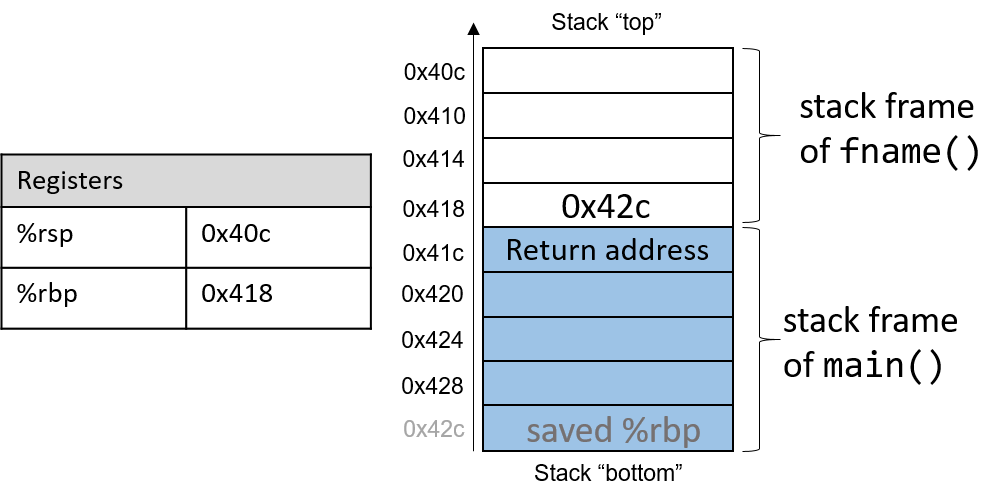
\includegraphics[scale=0.6]{img/stackFrame.png}
        \caption{The current active frame belongs to the callee function (fname). The memory between the stack pointer and the frame pointer is used for local variables. The stack pointer moves as local values are pushed and popped from the stack. In contrast, the frame pointer remains relatively constant, pointing to the beginning (the bottom) of the current stack frame. As a result, compilers like GCC commonly reference values on the stack relative to the frame pointer. In Figure 1, the active frame is bounded below by the base pointer of fname, which is stack address 0x418. The value stored at address 0x418 is the "saved" \texttt{\%rbp} value (0x42c), which itself is an address that indicates the bottom of the activation frame for the main function. The top of the activation frame of main is bounded by the return address, which indicates where in the main function program execution resumes once the callee function fname finishes executing. }
        \label{fig:stack_frame_management}
      \end{figure}


      Once we have done this we are really done. Formally, this is called Turing complete (?). 

      \begin{definition}[Control Transfers]
        We list some. 
        \begin{enumerate}
          \item Push 
          \item Pop 
          \item Call to call a function 
          \item Return to return from a function 
          \item Continue 
          \item Get out of stack with leave.  
        \end{enumerate}
      \end{definition}

      \begin{example}[Control Transfer Example]
        We show this with a minimal example with psuedocode. 
      \end{example}

    \subsubsection{Multiple Functions}

      Now what happens if there are multiple functions calling each other? Take a look at the following example with two functions. 

      \begin{example}[Multiple Functions Example]
        
      \end{example}

      There is a bit of a concern here from the previous example. The main function had two functions that returned two values. As the subfunction stack frame is removed from the stack, the return value is stored in the \texttt{\%rax} register. If another function is called right after, then the return value of the second function will overwrite that of the previous one. This was not a problem in the previous example since the return value of the \texttt{assign} function was not used. However, if it was, then the return value of the \texttt{adder} function would have overwritten it. This is known as register saving. 
      \begin{enumerate}
        \item For \textbf{caller-saved registers}, the caller function is responsible for saving the value of the register before calling a function and restoring it after the function returns. The caller should save values in its stack frame before calling the callee function, e.g. by pushing all the return values of each callee in the caller stack frame. Then it will restore values after the call. 

        \begin{center}
          \textit{Therefore, if we have a set of registers $\{\texttt{\%reg}\}$, the caller must take everything and push them in the caller stack frame. Then it will restore them after the call.}
        \end{center}

        \item For \textbf{callee-saved registers}, it is the callee's responsibility to save any data in these registers before using the registers. 

          \begin{center} 
            \textit{Therefore, if we have a set of registers $\{\texttt{\%reg}\}$, then inside the callee stack frame, the callee must take everything and push them in the callee stack frame. Once it computes the final return value, then it will restore all the saved register values from the callee stack frame back into the registers for the caller to use.}
          \end{center}
      \end{enumerate}

      Ideally, we want \textit{one} calling convention to simply separate implementation details between caller and callee. In general, however, neither is best. If the caller isn't using a register, then caller-save is better, and if callee doesn't need a register, then callee-save is better. If we do need to save, then callee save generally makes smaller programs, so we compromise and use a combination of both caller-save and callee-save. 

    \subsubsection{x86-64 Instructions}

      Let's talk about moving instructions first. 

      \begin{definition}[mov]
        Let's talk about the \texttt{mov} instruction which copies data from the source to the destination (the data in the source still remains!) and has the syntax 
        \begin{equation}
          \texttt{mov\_ src, dest}
        \end{equation}
        \begin{enumerate}
          \item The source can be a register (\texttt{\%rsi}), a value (\texttt{\$0x4}), or a memory address (\texttt{0x4}).
          \item The destination can be a register or a memory address. 
          \item The \texttt{\_} is defined to be one of the size operands, which determine how big the data is. For example, we can call \texttt{movq} to move 8 bytes of data (which turns about to be the maximum size of a register). 
        \end{enumerate}
        A good diagram to see is the following: 
        \begin{center}  
          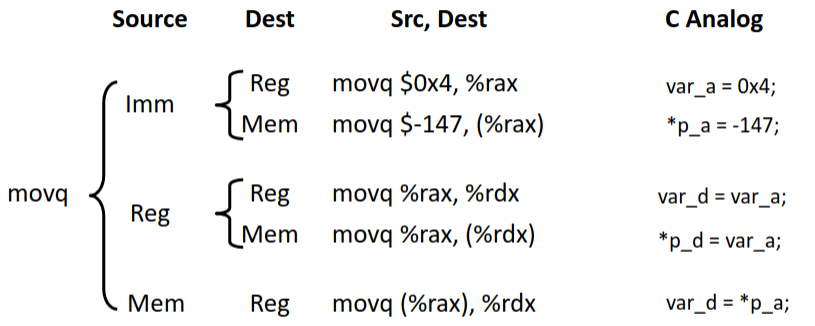
\includegraphics[scale=0.5]{img/movq.png}
        \end{center} 
      \end{definition}

      Even with just the mov instruction, we can look at a practical implementation of a C program in Assembly. 

      \begin{example}[Swap Function]
        Let us take a look at a function that swaps two integers. Let's see what they do. 
        \begin{enumerate}
          \item In C, we dereference both \texttt{xp} and \texttt{yp} (note that they are pointers to longs, so they store 8 bytes), and assign these two values to two temporary variables. Then, we assign the value of \texttt{yp} to \texttt{xp} and the value of \texttt{xp} to \texttt{yp}.
          \item In Assembly, we first take the registers \texttt{\%rdi} and \texttt{\%rsi}, which are the 1st and 2nd arguments of the function, dereference them with the parantheses, and store them in the temporary registers \texttt{\%rax} and \texttt{\%rdx}. Then, we store the value of \texttt{\%rdx} into the memory address of \texttt{\%rdi} and the value of \texttt{\%rax} into the memory address of \texttt{\%rsi}. Note that the input values (the actual of )
        \end{enumerate}

        \noindent\begin{minipage}{.5\textwidth}
        \begin{lstlisting}[]{Code}
          void swap(long *xp, long *yp) {
            long t0 = *xp;
            long t1 = *yp;
            *xp = t1;
            *yp = t0;
          }
        \end{lstlisting}
        \end{minipage}
        \hfill
        \begin{minipage}{.49\textwidth}
        \begin{lstlisting}[]{Output}
          swap:
            movq (%rdi), %rax
            movq (%rsi), %rdx
            movq %rdx, (%rdi)
            movq %rax, (%rsi)
            ret
        \end{lstlisting}
        \end{minipage}
      \end{example}

      \begin{definition}[movz and movs]
        The \texttt{movz} and \texttt{movs} instructions are used to move data from the source to the destination, but with zero and sign extension, respectively. It is used to copy from a smaller source value to a larger destination, with the syntax 
        \begin{align*}
          \texttt{movz\_\_ src, dest} \\ 
          \texttt{movs\_\_ src, dest} 
        \end{align*}
        where the first $\_$ is the size of the source and the second $\_$ is the size of the destination. 
        \begin{enumerate}
          \item The source can be from a memory or register. 
          \item The destination must be a register. 
        \end{enumerate}
      \end{definition}

      \begin{example}[Simple example with movz]
        Take a look at the code below. 
        \begin{lstlisting}
          movzbq %al, %rbx
        \end{lstlisting}
        The \texttt{\%al} represents the last byte of the \texttt{\%rax} register. It is 1 byte long. The \texttt{\%rbx} register is 8 bytes long, so we can fill in the rest of the 7 bytes with zeros. 
        \begin{center}  
          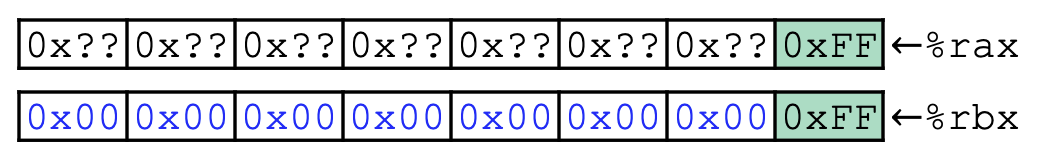
\includegraphics[scale=0.5]{img/movzbq.png}
        \end{center}
      \end{example}

      \begin{example}[Harder example with movs]
        Take a look at the code below. 
        \begin{lstlisting}
          movsbl (%rax), %ebx
        \end{lstlisting}
        You want to move the value at the memory address in \texttt{\%rax} into \texttt{\%ebx}. Since the source size is set to 1 byte, you take that byte, say it is \texttt{0x80}, from the memory, and then sign extend it (by a size of 4 bytes!) into \texttt{\%ebx}. Note that therefore, the first four bytes of \texttt{\%rbx} will not be affected since it's not a part of \texttt{\%ebx}. An exception to this is that in x86-64, any instruction that generates a 32-bit long word value for a register also sets the high-order 32 bits of the register to 0, so this ends up clearing the first 4 bytes to 0. 
        \begin{center}  
          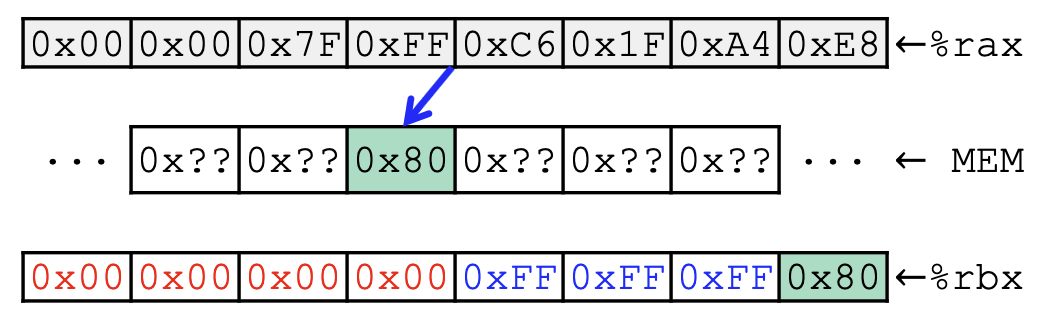
\includegraphics[scale=0.5]{img/movsbl.png}
        \end{center}
      \end{example}

      Now we can talk about control transfer. Say that you have the following C and Assembly code. 
      
      \begin{figure}[H]
        \centering 
        \noindent\begin{minipage}{.5\textwidth}
        \begin{lstlisting}[]{Code}
          int add(int x) {
            return x + 2; 
          }

          int main() {
            int a = 2; 
            int b = add(a); 
            return 0; 
          }
        \end{lstlisting}
        \end{minipage}
        \hfill
        \begin{minipage}{.49\textwidth}
        \begin{lstlisting}[]{Output}
          add: 
            movq %rdi, %rax 
            addq $2, %rax 
            ret 
          main:
            movq $3, $rdi 
            call add 
            movq $0, %rax 
            ret 
        \end{lstlisting}
        \end{minipage}
        \caption{A simple function. } 
        \label{fig:stack_example}
      \end{figure}

      If you go through the instructions, you see that in main, you first move \texttt{\$3} into the \texttt{\%rdi} register. Then, you call the \texttt{add} function, and within it you also have the \texttt{\%rdi} register. This is a conflict in the register, and we don't want to simply overwrite the value of \texttt{\%rdi} in the \texttt{main} function. Simply putting it to another register isn't a great idea since we can't always guarantee that it will be free. Therefore, we must use the memory itself. 

      Recall the stack, which we can think of as a giant array in which data gets pushed and popped in a last-in-first-out manner. The stack is used to store data and return addresses, and is used to manage function calls. Visually, we want to think of the elements getting pushed in from the bottom (upside down) towards lower memory addresses. 

      \begin{definition}[Stack Pointer]
        Note that every time we want to push or pop something from the stack, we must know \textit{where} to push or pop it. This is where the \textbf{stack pointer} comes in. It is a special register that always points to the top of the stack, and is used to keep track of the stack.
      \end{definition}

      \begin{definition}[Push and Pop]
        The \texttt{push} and \texttt{pop} instructions are used to push and pop data onto and off the stack, respectively. 
        \begin{align*}
          \texttt{push\_ src} && \texttt{rsp = rsp - 8; Mem[rsp] = src} \\
          \texttt{pop\_ dest} && \texttt{dest = Mem[rsp]; rsp = rsp + 8} 
        \end{align*}
        \begin{enumerate}
          \item When we push the source, we fetch the value at the source and store it at the memory address pointed to by the stack pointer \texttt{\%rsp}. Then, we decrement \texttt{\%rsp} by 8.
          \item When we pop from the stack, we fetch the value at the memory address pointed to by the stack pointer \texttt{\%rsp} and store it in the destination. Then, we increment \texttt{\%rsp} by 8.
        \end{enumerate}
        Note that no matter what the size of the operand, we always subtract 8 from the stack pointer. This is because the stack grows downwards, and we want to make sure that the next element is pushed into the next available space.
      \end{definition}

      Note that the register \texttt{\%rsp} is the stack pointer, which points to the top of the stack. The stack is used to store data and return addresses, and is used to manage function calls. 

      \begin{definition}[Push and Pop]
        The \texttt{push} and \texttt{pop} instructions are used to push and pop data onto and off the stack, respectively. 
        \begin{align*}
          \texttt{push\_ src} && \texttt{rsp = rsp - 8; Mem[rsp] = src} \\
          \texttt{pop\_ dest} && \texttt{dest = Mem[rsp]; rsp = rsp + 8} 
        \end{align*}
        The \texttt{\_} is a size operand, which determines how big the data is.
      \end{definition}

      \begin{definition}[Call and Ret]
        The \texttt{call} instruction pushes the return address onto the stack and jumps to the function. The \texttt{ret} instruction pops the return address from the stack and jumps to it.
      \end{definition}

      We also talked about how there is instruction code that is even below the stack that is stored. This is where all the machine code/assembly is stored, and we want to find out where we are currently at in this code. This is done with the program counter. 

      \begin{definition}[Program Counter, Instruction Pointer] 
        The \textbf{program counter}, or \textbf{instruction pointer}, is a special register \textbf{rip} that points to the current instruction in the program. It is used to keep track of the next instruction to be executed.
      \end{definition}

      Let's go through one long example to see in detail how this is calculated. 
      
      \begin{example}[Evaluating a Function]
        Say that we have the following C code. 
        \begin{lstlisting}
          int adder2(int a) {
            return a + 2; 
          }

          int main() {
            int x = 40; 
            x = adder2(x); 
            printf("x is: %d\n", x);
            return 0; 
          }
        \end{lstlisting}
        When we compile this program, we can view its full assembly code by calling \texttt{objdump -d a.out}. The output is quite long, so we will focus on the instruction for the \texttt{adder2} function. 
        \begin{figure}[H]
          \centering 
          \begin{lstlisting}
            0000000000400526 <adder2>:
            400526:       55                      push   %rbp
            400527:       48 89 e5                mov    %rsp,%rbp
            40052a:       89 7d fc                mov    %edi,-0x4(%rbp)
            40052d:       8b 45 fc                mov    -0x4(%rbp),%eax
            400530:       83 c0 02                add    $0x2,%eax
            400533:       5d                      pop    %rbp
            400534:       c3                      retq
          \end{lstlisting}
          \caption{The output of objdump for the \texttt{adder2} function. The leftmost column represents the addresses (in hex) of where the actual instructions lie. The second column represents the machine code that is being executed. The third column represents the assembly code.}
          \label{fig:adder2} 
        \end{figure}
        Note some things. Since \texttt{adder2} is taking in an integer input value, we want to load it into the lower 32 bits (4 bytes) of the \texttt{\%rdi} register, which is the first parameter. So we use \texttt{\%edi}. Likewise for the return value, we want to output an int so we use \texttt{\%eax} rather than \texttt{\%rax}. Let's go through some of the steps. 
        \begin{enumerate}
          \item By the time we get into calling \texttt{adder2}, we can take a look at the relevant registers. 

            \begin{center}
              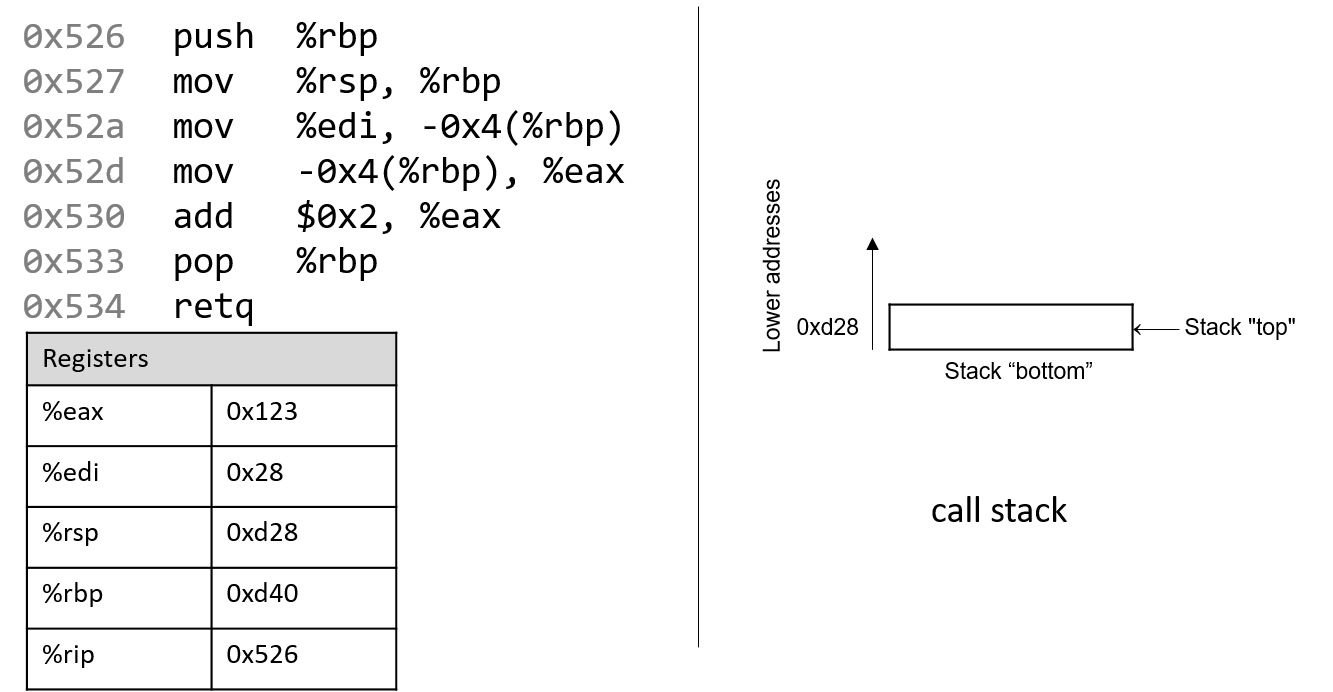
\includegraphics[scale=0.5]{img/ex1_1.png}
            \end{center}
            \begin{enumerate}
              \item First, the \texttt{\%eax} is filled with garbage, which are leftovers from previous programs that haven't been overwritten yet. 
              \item Second, the \texttt{\%edi=0x28} since we have set \texttt{x=40} in \texttt{main}, before calling \texttt{adder2}, so it lingers on. 
              \item \texttt{\%rsp=0xd28} since that is where the top of the stack is. 
              \item \texttt{\%rbp=0xd40} 
              \item \texttt{\%rip=0x526} since that is where we are currently at in our instruction (we are about to do it, but haven't done it yet). 
            \end{enumerate}

          \item When we execute the first line of code, we simply push the value at \texttt{\%rbp} into the stack. The top of the stack gets decremeneted by 8 and the value at \texttt{\%rbp} is stored there. This means that the top of the stack is at \texttt{\%rsp=0xd20} and the next instruction will be at \texttt{\%rip=0x527}.  

            \begin{center}
              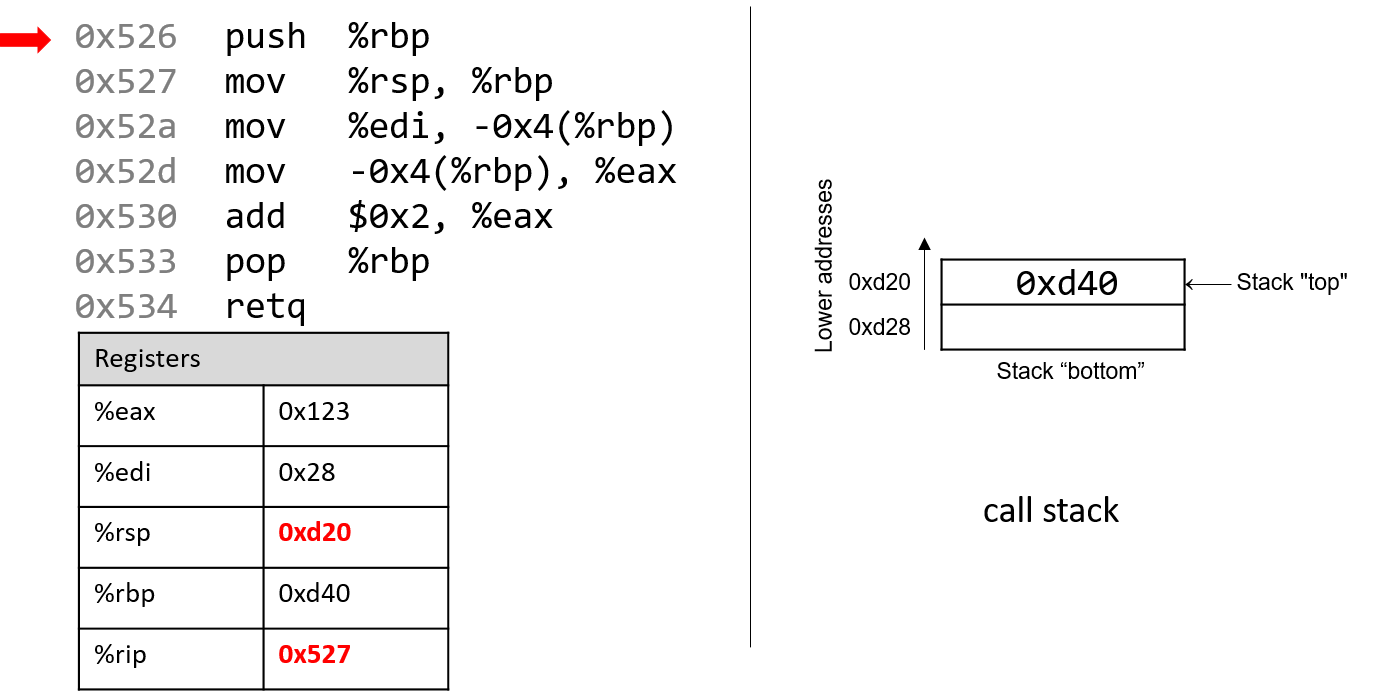
\includegraphics[scale=0.5]{img/ex1_2.png}
            \end{center}

          \item The reason we have pushed \texttt{\%rbp} onto the stack is that we want to save it before it gets overwritten by this next execution. We basically move the value of \texttt{\%rsp} into \texttt{\%rbp}, and the \texttt{\%rip} advances to the next instruction. \texttt{\%rip} moves to the next instruction. 

            \begin{center}
              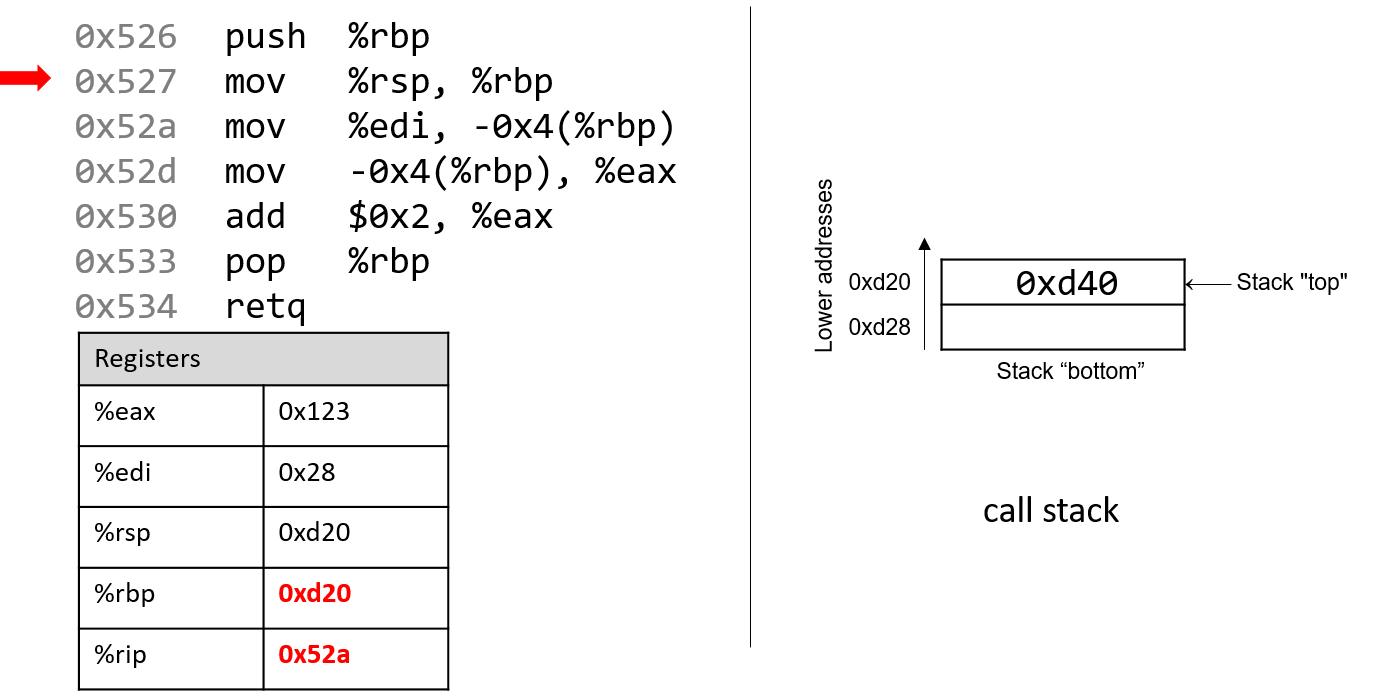
\includegraphics[scale=0.5]{img/ex1_3.png}
            \end{center}

          \item Now we want to take our first argument \texttt{\%edi} and store it in memory. Note that since this is 4 bytes, we can move this value into memory that is 4 bytes below the stack (\texttt{-0x4(\%rbp)}). Note that the storing the value of \texttt{\%edi} into memory doesn't affect the stack pointer \texttt{\%rsp}. As far as the program is concerned, the top of this stack is still address \texttt{0xd20}. 

            \begin{center}
              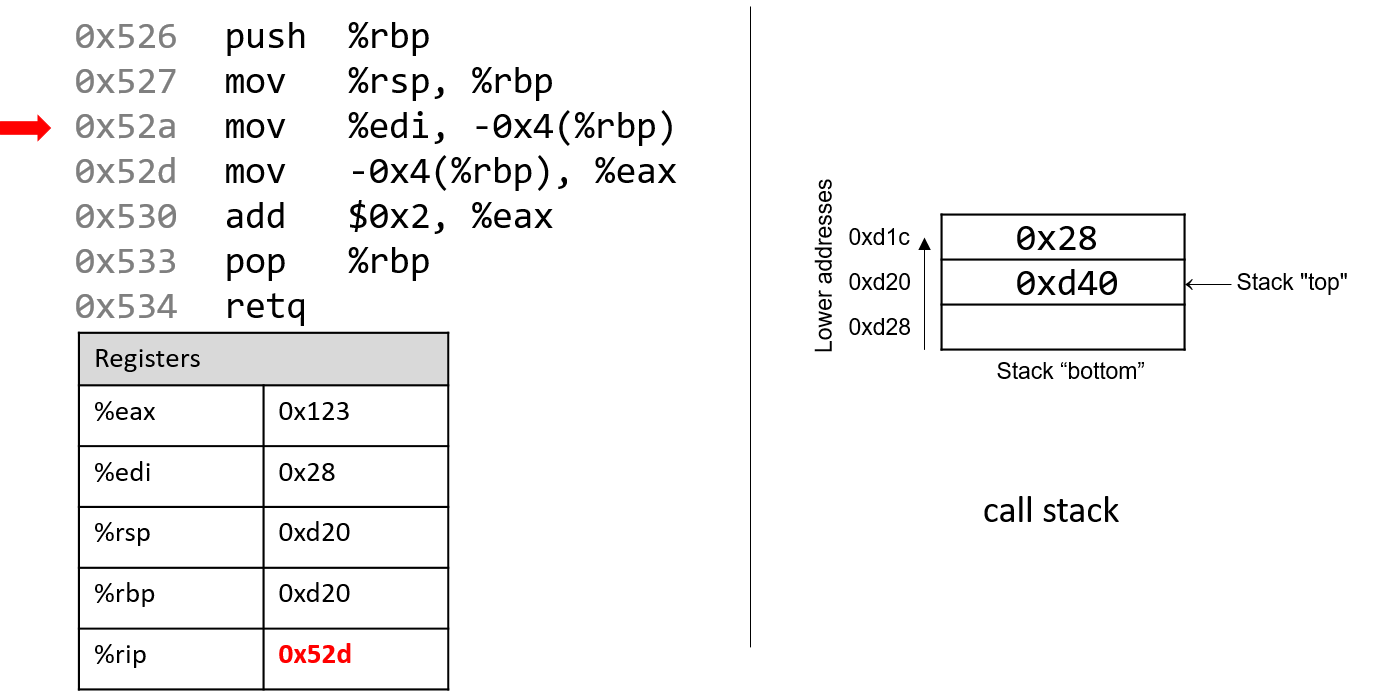
\includegraphics[scale=0.5]{img/ex1_4.png}
            \end{center}

          \item The next instruction simply goes into memory 4 bytes below the stack pointer, takes the value there, and stores it into \texttt{\%eax}. This is the value of \texttt{\%edi} that we just stored. This may seem redundant since we are making a round trip to memory and back to ultimately move the value of \texttt{\%edi} into \texttt{\%eax}, but compilers are not smart and just follow these instructions. 

            \begin{center}
              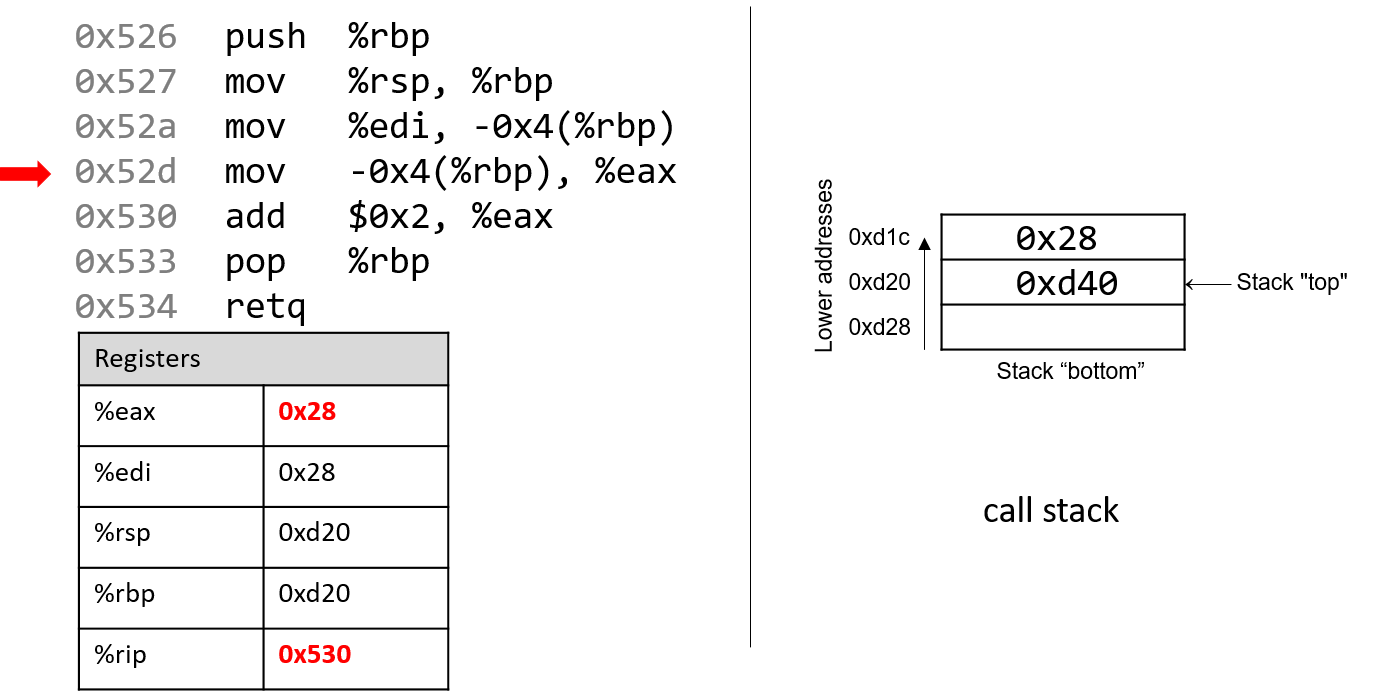
\includegraphics[scale=0.5]{img/ex1_5.png}
            \end{center}

          \item Finally, we add the value \texttt{\$0x2} to \texttt{\%eax} and store it back into \texttt{\%eax}. 

            \begin{center}
              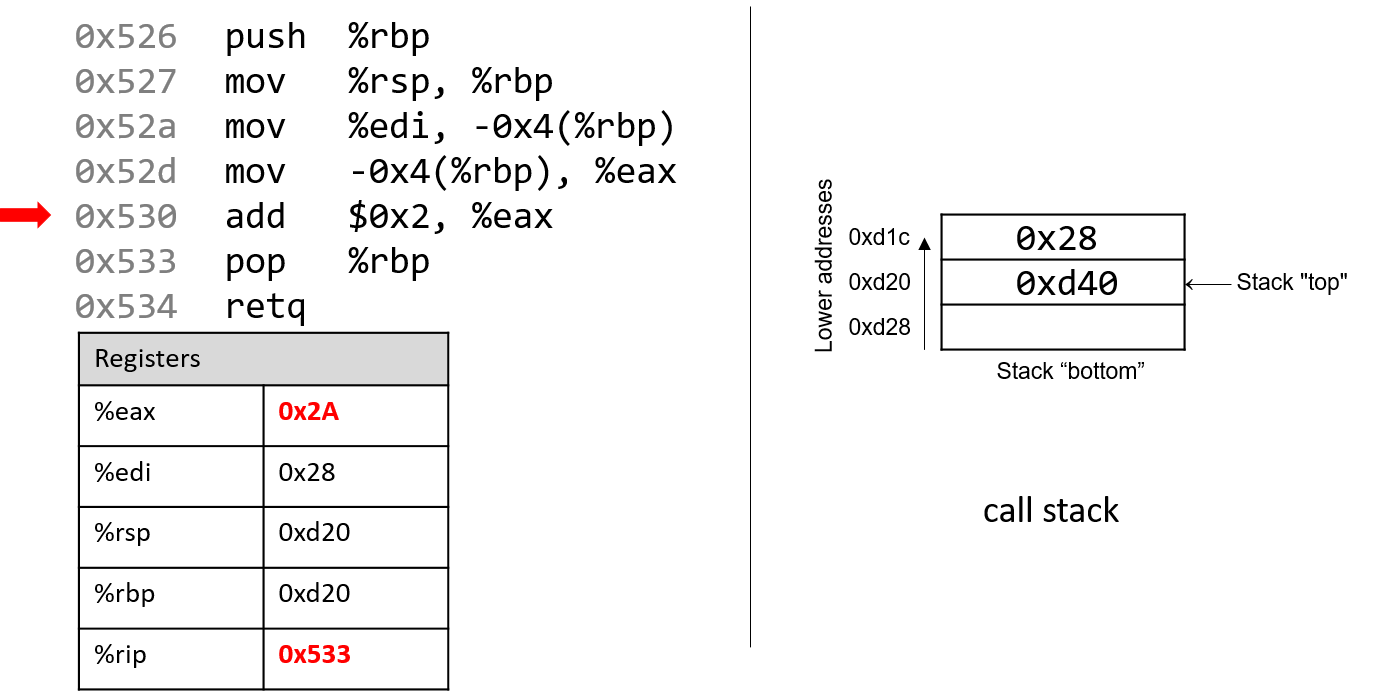
\includegraphics[scale=0.5]{img/ex1_6.png}
            \end{center}

          \item Finally, we pop the value at the top of the stack and store it into \texttt{\%rbp}. Note that this is \textit{not} the value \texttt{0x28}. It is simply the value that is stored at \texttt{\%rsp=0xd20}, which is \texttt{(\%rsp)=0xd40}. 

            \begin{center}
              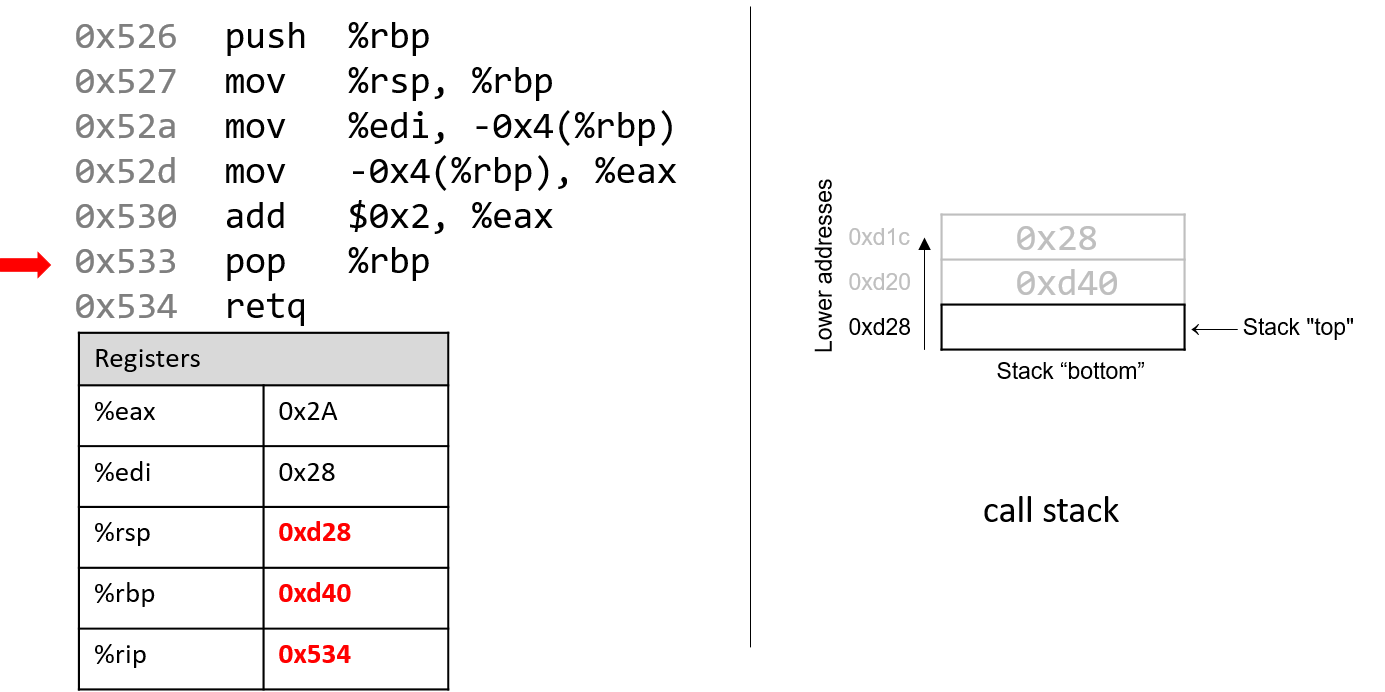
\includegraphics[scale=0.5]{img/ex1_7.png}
            \end{center}

          \item Finally, we return the value with \texttt{retq}. 
        \end{enumerate}
      \end{example}

      Note that the final values in the registers \texttt{\%rsp} and \texttt{\%rip} are \texttt{0xd28} and \texttt{0x534}, respectively, which are the same values as when the function started executing! This is normal and expected behavior with the call stack, which just stores temporary variable sand data of each function as it executes a program. Once a function completes executing, the stack returns to the state it was in prior to the function call. Therefore, it is common to see the following two instructions at the beginning of a function: 
      \begin{lstlisting}
        push %rbp 
        mov %rsp, %rbp
      \end{lstlisting}
      and the following two at the end of a function 
      \begin{lstlisting}
        pop %rbp 
        retq
      \end{lstlisting}

      Now arithemtic operations are quite simple.

      \begin{definition}[Add, Subtract, Multiply]
        The \textbf{add} and \textbf{sub} instructions are used to add and subtract data from the destination. 
        \begin{align*}
          \texttt{add\_ src, dest} && \texttt{dest = dest + src} \\
          \texttt{sub\_ src, dest} && \texttt{dest = dest - src}
        \end{align*}
        The \textbf{imul} instruction is used to multiply data between the source and destination and store it in the destination.  
        \begin{align*}
          \texttt{imul\_ src, dest} && \texttt{dest = dest * src} 
        \end{align*}
        Again the \texttt{\_} is a size operand, which determines how big the data is. 
      \end{definition}

      \begin{definition}[Increment, Decrement]
        The \textbf{inc} and \textbf{dec} instructions are used to increment and decrement the value in the destination. 
        \begin{align*}
          \texttt{inc\_ dest} && \texttt{dest = dest + 1} \\
          \texttt{dec\_ dest} && \texttt{dest = dest - 1}
        \end{align*}
      \end{definition}

      \begin{definition}[Negative]
        The \textbf{neg} instruction is used to negate the value in the destination. 
        \begin{align*}
          \texttt{neg\_ dest} && \texttt{dest = -dest} 
        \end{align*}
      \end{definition}

      \begin{example}[Basic Arithmetic Function]
        The following represents the same program in C and in assembly. Let's go through each one: 
        \begin{enumerate}
          \item In C, we first initialize \texttt{a = 4}, then \texttt{b = 8}, add them together to get \texttt{c}, and then return \texttt{c}.
          \item In Assembly, we move the value $4$ to the \texttt{\%rax} register, then move the value $8$ to the \texttt{\%rbx} register, add the two values together to store it into \texttt{\%rax}, and then return the value in the \texttt{\%rax} register.
        \end{enumerate}
        \noindent\begin{minipage}{.5\textwidth}
        \begin{lstlisting}[]{Code}
          int main() {
            int a = 4, b = 8; 
            int c = a + b; 
            return c; 
          }
        \end{lstlisting}
        \end{minipage}
        \hfill
        \begin{minipage}{.49\textwidth}
        \begin{lstlisting}[]{Output}
          main:
            movq $4, %rax
            movq $8, %rbx
            addq %rbx, %rax
            ret
        \end{lstlisting}
        \end{minipage}
        It is slightly different in Assembly since rather than storing $4$ in some intermediate register, we immediately store it in the return register. In a way it is more optimized, and this is what the compiler does for you so that as few registers are used. 
      \end{example}

      A shorthand way to do this is with \texttt{lea}, which stands for load effective address. 

      \begin{definition}[Load Effective Address]
        The \textbf{lea} instruction is used to load the effective address of the source into the destination. For now, we will focus on the arithmetic operations that it can do
        \begin{align*}
          \texttt{lea\_ (src1, src2), dest} && \texttt{dest = src1 + src2}  \\ 
          \texttt{lea\_ (src1, src2, scale), dest} && \texttt{dest = src1 + src2*scale}  \\ 
          \texttt{lea\_ const(src1, src2), dest} && \texttt{dest = src1 + src2 + const} \\ 
          \texttt{lea\_ const(src1, src2, scale), dest} && \texttt{dest = src1 + src2*scale + const}
        \end{align*}
        This is useful for doing arithmetic operations on the address of a variable.
      \end{definition}

      \begin{definition}[Bitwise]
        The \textbf{and}, \textbf{or}, \textbf{xor}, and \textbf{not} instructions are used to perform bitwise operations on the source and destination. 
        \begin{align*}
          \texttt{and src, dest} && \texttt{dest = dest \& src}  \\
          \texttt{or src, dest} && \texttt{dest = dest | src}  \\
          \texttt{xor src, dest} && \texttt{dest = dest \^ src}  \\
          \texttt{neg dest} && \texttt{dest = -dest}  \\
          \texttt{not dest} && \texttt{dest = $\sim$dest}  
        \end{align*}
      \end{definition}

      \begin{definition}[Arithmetic and Logical Bit Shift]
        The \texttt{sal} arithmetic instruction is used to shift the bits of the destination to the left by the number of bits specified in the source. The \texttt{shr} instruction is used to shift the bits of the destination to the right by the number of bits specified in the source.
        \begin{align*}
          \texttt{sal src, dest} && \texttt{dest = dest << src}  \\
          \texttt{shr src, dest} && \texttt{dest = dest >> src}
        \end{align*}
        The \texttt{sar} instruction is used to shift the bits of the destination to the right by the number of bits specified in the source, and fill the leftmost bits with the sign bit. The \texttt{shl} instruction is used to shift the bits of the destination to the left by the number of bits specified in the source, and fill the rightmost bits with zeros. 
        \begin{align*}
          \texttt{sar src, dest} && \texttt{dest = dest >> src}  \\
          \texttt{shl src, dest} && \texttt{dest = dest << src}
        \end{align*}
      \end{definition}

      \begin{example}[Harder Arithmetic Example]
        The following two codes are equivalent. 

        \noindent\begin{minipage}{.5\textwidth}
        \begin{lstlisting}[]{Code}
          long arith(long x, long y, long z) {
            long t1 = x + y; 
            long t2 = z + t1; 
            long t3 = x + 4; 
            long t4 = y * 48; 
            long t5 = t3 + t4;
            long rval = t2 * t5; 
            return rval; 
          }
          .
          .
          .
          .
          .
        \end{lstlisting}
        \end{minipage}
        \hfill
        \begin{minipage}{.49\textwidth}
        \begin{lstlisting}[]{Output}
          arith: 
            # rax/t1 = x + y
            leaq  (%rdi, %rsi), %rax
            # rax/t2 = z + t1
            addq  %rdx, %rax
            #rdx = 3 * y 
            leaq  (%rsi, %rsi, 2), %rdx
            #rdx/t4 = (3*y) * 16
            salq  $4, %rdx 
            #rcx/t5 = x + t4 + 4
            leaq  4(%rdi, %rdi), %rcx 
            # rax/rval = t5 * t2
            imulq %rcx, %rax 
            ret 
        \end{lstlisting}
        \end{minipage}
      \end{example}
  
      The final thing in our list is condition codes. 

      Sometimes, we want to move (really copy) some value to another register if some condition is met. This is where we use conditional moves. These conditions are met by the flags register, which is a special register that stores the status of the last operation. It is the value of these flags that determine whether all future conditional statements are met in assembly. 
      
      \begin{definition}[Condition Code Flags]
        The flags register in the x86 CPU keeps 4 \textit{condition code} flag bits internally. Think of these as status flags that are \textit{implicitly} set by the most recent arithmetic operation (think of it as side effects). Note that condition codes are NOT set by \texttt{lea} or \texttt{mov} instructions! 
        \begin{enumerate}
          \item \textbf{Zero Flag}: if the last operation resulted in a zero value.
          \item \textbf{Sign Flag}: if the last operation resulted in a negative value (i.e. the most significant bit is 1).
          \item \textbf{Overflow Flag}: if the last operation resulted in a signed overflow.
          \item \textbf{Carry Flag}: if the last operation resulted in a carry out of the most significant bit, i.e. an unsigned overflow. 
        \end{enumerate}
        Every operation may or may not changes these flags to test for zero or nonzero, positive or negative, or overflow conditions, and combinations of these flags express the full range of conditions and cases, e.g. for signed and unsigned values. 
      \end{definition}

      \begin{example}[Zero Flag]
        If the code below was just run, then ZF would be set to 1. 
        \begin{lstlisting}
          movq $2, %rax 
          subq $2, %rax
        \end{lstlisting}
      \end{example}

      \begin{example}[Sign Flag]
        If the code below was just run, then SF would be set to 1. 
        \begin{lstlisting}
          movq $2, %rax 
          subq $4, %rax
        \end{lstlisting}
      \end{example}

      \begin{example}[Overflow Flag]
        If either code below was just run, then OF would be set to 1. 

        \noindent\begin{minipage}{.5\textwidth}
        \begin{lstlisting}[]{Code}
          movq $0x7fffffffffffffff, %rax 
          addq $1, %rax
        \end{lstlisting}
        \end{minipage}
        \hfill
        \begin{minipage}{.49\textwidth}
        \begin{lstlisting}[]{Output}
          movq 0x8000000000000000, %rax 
          addq 0xffffffffffffffff, %rax
        \end{lstlisting}
        \end{minipage}
        This is because in the left in signed arithmetic, we have a positive + positive = negative (result is \texttt{0x8000000000000000}), which is a signed overflow. Furthermore, in the right we have negative + negative = positive (result is \texttt{0x7fffffffffffffff}). 
      \end{example}

      \begin{example}[Carry Flag]
        If the code below was just run, then CF would be set to 1. 
        \begin{lstlisting}
          movq $0xffffffffffffffff, %rax 
          addq $1, %rax
        \end{lstlisting}
        This is because the result is $0x0$, which is a carry out of the most significant bit and an unsigned overflow.
      \end{example}

      It would be tedious to always set these flags manually, so there are two methods that can be used to \textit{explicitly} set these flags. 

      \begin{definition}[Compare]
        The \textbf{cmp} instruction is used to perform a subtraction between the source and destination, and set the flags accordingly, but it does not store the result.
        \begin{align*}
          \texttt{cmp\_ src, dest} && \texttt{dest - src} 
        \end{align*}
        The following flags are set if the conditions are met: 
        \begin{enumerate}
          \item \textbf{ZF = 1} if \texttt{dest == src} 
          \item \textbf{SF = 1} if \texttt{dest < src} (MSB is 1) 
          \item \textbf{OF = 1} if signed overflow 
          \item \textbf{CF = 1} if unsigned overflow
        \end{enumerate}
      \end{definition}

      \begin{definition}[Test]
        The \textbf{test} instruction is used to perform a bitwise AND operation between the source and destination, and set the flags accordingly. 
        \begin{align*}
          \texttt{test\_ src, dest} && \texttt{dest \& src} 
        \end{align*}
        The following flags are set if the conditions are met. Note that you can't have carry out (CF) or overflow (OF) if these flags are set. 
        \begin{enumerate}
          \item \textbf{ZF = 1} if \texttt{dest \& src == 0} 
          \item \textbf{SF = 1} if \texttt{dest \& src < 0} (MSB is 1) 
        \end{enumerate}
      \end{definition}

      \begin{example}[Compare] 
        Assuming that \texttt{\%al = 0x80} and \texttt{\%bl = 0x81}, which flags are set when we execute \texttt{cmpb \%al, \%bl}? Well we must first compute 
        \begin{equation}
          \texttt{\%bl - \%al = 0x81 - 0x80 = 0x81 + $\sim$ 0x80 + 1 = 0x81 + 0x7F + 1 = 0x101 = 0x01}
        \end{equation}
        \begin{enumerate}
          \item CF=1 since the result is greater than 0xFF (i.e. larger than byte) 
          \item ZF=0 since the result is not 0 
          \item SF=0 since the MSB is 0, i.e. there is unsigned overflow
          \item OF=0 since there is no signed overflow
        \end{enumerate}
      \end{example}

      For conditional moves and jumps later shown, it basically uses these explicit sets and always compares them to $0$. We will see what this means later. 

      Finally, we can actually set a byte in a register to 1 or 0 based on the value of a flag. 

      \begin{definition}[Set]
        
      \end{definition}

      We can then talk about conditional moves and jumps.  

      \begin{definition}[Equality with 0]
        The \texttt{test} instruction is used to perform a bitwise AND operation between the source and destination, and set the flags accordingly. 
        \begin{align*}
          \texttt{test\_ src, dest} && \texttt{dest \& src} 
        \end{align*}
        The \texttt{sete} instruction is used to set the destination to 1 if the zero flag is set, and 0 otherwise. 
        \begin{align*}
          \texttt{sete\_ dest} && \texttt{dest = (ZF == 1) ? 1 : 0} 
        \end{align*}
        The \texttt{cmovne} instruction is used to move the source to the destination if the zero flag is not set. 
        \begin{align*}
          \texttt{cmovne\_ src, dest} && \texttt{dest = (ZF == 0) ? src : dest} 
        \end{align*}
      \end{definition}


      \begin{definition}[Jump]
        There are several jump instructions, but essentially they are used to jump to another part of the code. We can use the following mnemonic to jump to a label. 

        \begin{figure}[H]
          \centering 
          \begin{table}[H]
            \centering
            \begin{tabular}{|l|l|}
            \hline
            \textbf{Letter} & \textbf{Word} \\ \hline
            j & jump \\ \hline
            n & not \\ \hline
            e & equal \\ \hline
            s & signed \\ \hline
            g & greater (signed interpretation) \\ \hline
            l & less (signed interpretation) \\ \hline
            a & above (unsigned interpretation) \\ \hline
            b & below (unsigned interpretation) \\ \hline
            \end{tabular}
            \caption{Letter to Word Mapping}
            \label{table:letter_word_mapping}
          \end{table}
          \caption{Mnemonic for Jump Instructions} 
          \label{fig:jump_instructions_mnemonic}
        \end{figure}

        For completeness, we include all the jump instructions. 
          
        \begin{figure}[H]
          \centering 
          \begin{table}[H]
            \centering
            \begin{tabular}{|l|l|l|}
            \hline
            \textbf{Signed Comparison} & \textbf{Unsigned Comparison} & \textbf{Description} \\ \hline
            je (jz) & & jump if equal (==) or jump if zero \\ \hline
            jne (jnz) & & jump if not equal (!=) \\ \hline
            js & & jump if negative \\ \hline
            jns & & jump if non-negative \\ \hline
            jg (jnle) & ja (jnbe) & jump if greater (>) \\ \hline
            jge (jnl) & jae (jnb) & jump if greater than or equal (>=) \\ \hline
            jl (jnge) & jb (jnae) & jump if less (<) \\ \hline
            jle (jng) & jbe (jna) & jump if less than or equal (<=) \\ \hline
            \end{tabular}
            \caption{Comparison Instructions in Assembly}
            \label{table:comparison_instructions}
          \end{table}
          \caption{All jump instructions} 
          \label{fig:jump_instructions_all}
        \end{figure}
      \end{definition}

      \begin{definition}[int]
        The \texttt{int} instruction is used to generate a software interrupt. It is often used to invoke a system call.
      \end{definition}

      \begin{definition}[ret]
        The \texttt{ret} instruction is used to return from a function. It returns the value in the \texttt{\%rax} register. 
      \end{definition}

      Now we can have a basic idea of how if statements can be used as a sequence of conditionals and jump operators. Let's first look at the \textbf{goto} version of C. 

      \begin{definition}[Goto Syntax]
        The goto version processes instructions sequentially as long as there is no jump. This is useful because compilers translating code into assembly designate a jump when a condition is true. Contrast this behavior with the structure of an if statement, where a "jump" (to the else) occurs when conditions are not true. The goto form captures this difference in logic.
      \end{definition}

      \begin{figure}[H]
        \centering 
        \noindent\begin{minipage}{.5\textwidth}
        \begin{lstlisting}[]{Code}
          int getSmallest(int x, int y) {
            int smallest;
            if ( x > y ) { //if (conditional)
              smallest = y; //then statement
            }
            else {
              smallest = x; //else statement
            }
            return smallest;
          }
          .
          .
          .
          .
          .
        \end{lstlisting}
        \end{minipage}
        \hfill
        \begin{minipage}{.49\textwidth}
        \begin{lstlisting}[]{Output}
          int getSmallest(int x, int y) {
            int smallest;

            if (x <= y ) { //if (!conditional)
              goto else_statement;
            }
            smallest = y; //then statement
            goto done;

          else_statement:
            smallest = x; //else statement

          done:
            return smallest;
          }      
        \end{lstlisting}
        \end{minipage}
        \caption{C vs GoTo code of the same function. While GoTo code allows us to view C more like assmebly, it is generally not readable and is not considered best practice. } 
        \label{fig:c_vs_goto}
      \end{figure}

      Now let's see how if statements are implemented by taking a look at this function straight up in assembly. 

      \begin{figure}[H]
        \centering 
        \noindent\begin{minipage}{.4\textwidth}
        \begin{lstlisting}[]{Code}
          int getSmallest(int x, int y) {
            int smallest;
            if ( x > y ) { //if (conditional)
              smallest = y; //then statement
            }
            else {
              smallest = x; //else statement
            }
            return smallest;
          }
          .
        \end{lstlisting}
        \end{minipage}
        \hfill
        \begin{minipage}{.59\textwidth}
        \begin{lstlisting}[]{Output}
          Dump of assembler code for function getSmallest:
          0x40059a <+4>:   mov    %edi,-0x14(%rbp)
          0x40059d <+7>:   mov    %esi,-0x18(%rbp)
          0x4005a0 <+10>:  mov    -0x14(%rbp),%eax
          0x4005a3 <+13>:  cmp    -0x18(%rbp),%eax
          0x4005a6 <+16>:  jle    0x4005b0 <getSmallest+26>
          0x4005a8 <+18>:  mov    -0x18(%rbp),%eax
          0x4005ae <+24>:  jmp    0x4005b9 <getSmallest+35>
          0x4005b0 <+26>:  mov    -0x14(%rbp),%eax
          0x4005b9 <+35>:  pop    %rbp
          0x4005ba <+36>:  retq
        \end{lstlisting}
        \end{minipage}
        \caption{Assembly code of a simple if statement} 
        \label{fig:if_statement}
      \end{figure}

      Again, note that since we are working with int types, the respective parameter registers are \texttt{\%edi} and \texttt{\%esi}, the respective lower 32-bits of the registers \texttt{\%rdi} and \texttt{\%rsi}. Let's walk through this again. 
      \begin{enumerate}
        \item The first mov instruction copies the value located in register \%edi (the first parameter, x) and places it at memory location \%rbp-0x14 on the call stack. The instruction pointer (\%rip) is set to the address of the next instruction, or 0x40059d.
        \item The second mov instruction copies the value located in register \%esi (the second parameter, y) and places it at memory location \%rbp-0x18 on the call stack. The instruction pointer (\%rip) updates to point to the address of the next instruction, or 0x4005a0.
        \item The third mov instruction copies x to register \%eax. Register \%rip updates to point to the address of the next instruction in sequence.
        \item The cmp instruction compares the value at location \%rbp-0x18 (the second parameter, y) to x and sets appropriate condition code flag registers. Register \%rip advances to the address of the next instruction, or 0x4005a6.
        \item The jle instruction at address 0x4005a6 indicates that if x is less than or equal to y, the next instruction that should execute should be at location <getSmallest+26> and that \%rip should be set to address 0x4005b0. Otherwise, \%rip is set to the next instruction in sequence, or 0x4005a8.
      \end{enumerate}

      With the \texttt{cmov} instruction, this can be a lot shorter. With the gcc compiler with level 1 optimizations turned on, we can see that a lot of redundancies are turned off. 

      \begin{figure}[H]
        \centering 
        \begin{lstlisting}
          <getSmallest>:
          0x400546 <+0>: cmp    %esi,%edi      #compare x and y
          0x400548 <+2>: mov    %esi,%eax      #copy y to %eax
          0x40054a <+4>: cmovle %edi,%eax      #if (x<=y) copy x to %eax
          0x40054d <+7>: retq                  #return %eax
        \end{lstlisting}
        \caption{Compiled with \texttt{gcc -01 -o getSmallest getSmallest.c} } 
        \label{fig:if_statement_optimized}
      \end{figure}

      Like if statements, loops in assembly can be implementing using jump functions that revisit some instruction address based on the result on an evaluated condition. Let's take a look at a basic loop function. 

      \begin{figure}[H]
        \centering 
        \noindent\begin{minipage}{.5\textwidth}
        \begin{lstlisting}[]{Code}
          int sumUp(int n) {
            int total = 0;
            int i = 1;

            while (i <= n) {  
              total += i;   
              i++; 
            }
            return total;
          }
          .
          .
          .
          .
          .
          .
        \end{lstlisting}
        \end{minipage}
        \hfill
        \begin{minipage}{.49\textwidth}
        \begin{lstlisting}[]{Output}
          Dump of assembler code for function sumUp:
          0x400526 <+0>:   push   %rbp
          0x400527 <+1>:   mov    %rsp,%rbp
          0x40052a <+4>:   mov    %edi,-0x14(%rbp)
          0x40052d <+7>:   mov    $0x0,-0x8(%rbp)
          0x400534 <+14>:  mov    $0x1,-0x4(%rbp)
          0x40053b <+21>:  jmp    0x400547 <sumUp+33>
          0x40053d <+23>:  mov    -0x4(%rbp),%eax
          0x400540 <+26>:  add    %eax,-0x8(%rbp)
          0x400543 <+29>:  add    $0x1,-0x4(%rbp)
          0x400547 <+33>:  mov    -0x4(%rbp),%eax
          0x40054a <+36>:  cmp    -0x14(%rbp),%eax
          0x40054d <+39>:  jle    0x40053d <sumUp+23>
          0x40054f <+41>:  mov    -0x8(%rbp),%eax
          0x400552 <+44>:  pop    %rbp
          0x400553 <+45>:  retq
        \end{lstlisting}
        \end{minipage}
        \caption{Simple loop function in C and assembly. } 
        \label{fig:loop_function}
      \end{figure}

      Finally, we want to let the reader know the convention of calle and caller saved registers. The compiler tries to pick these registers, and by convention in x86, we have the following. 

      \begin{figure}[H]
        \centering 
        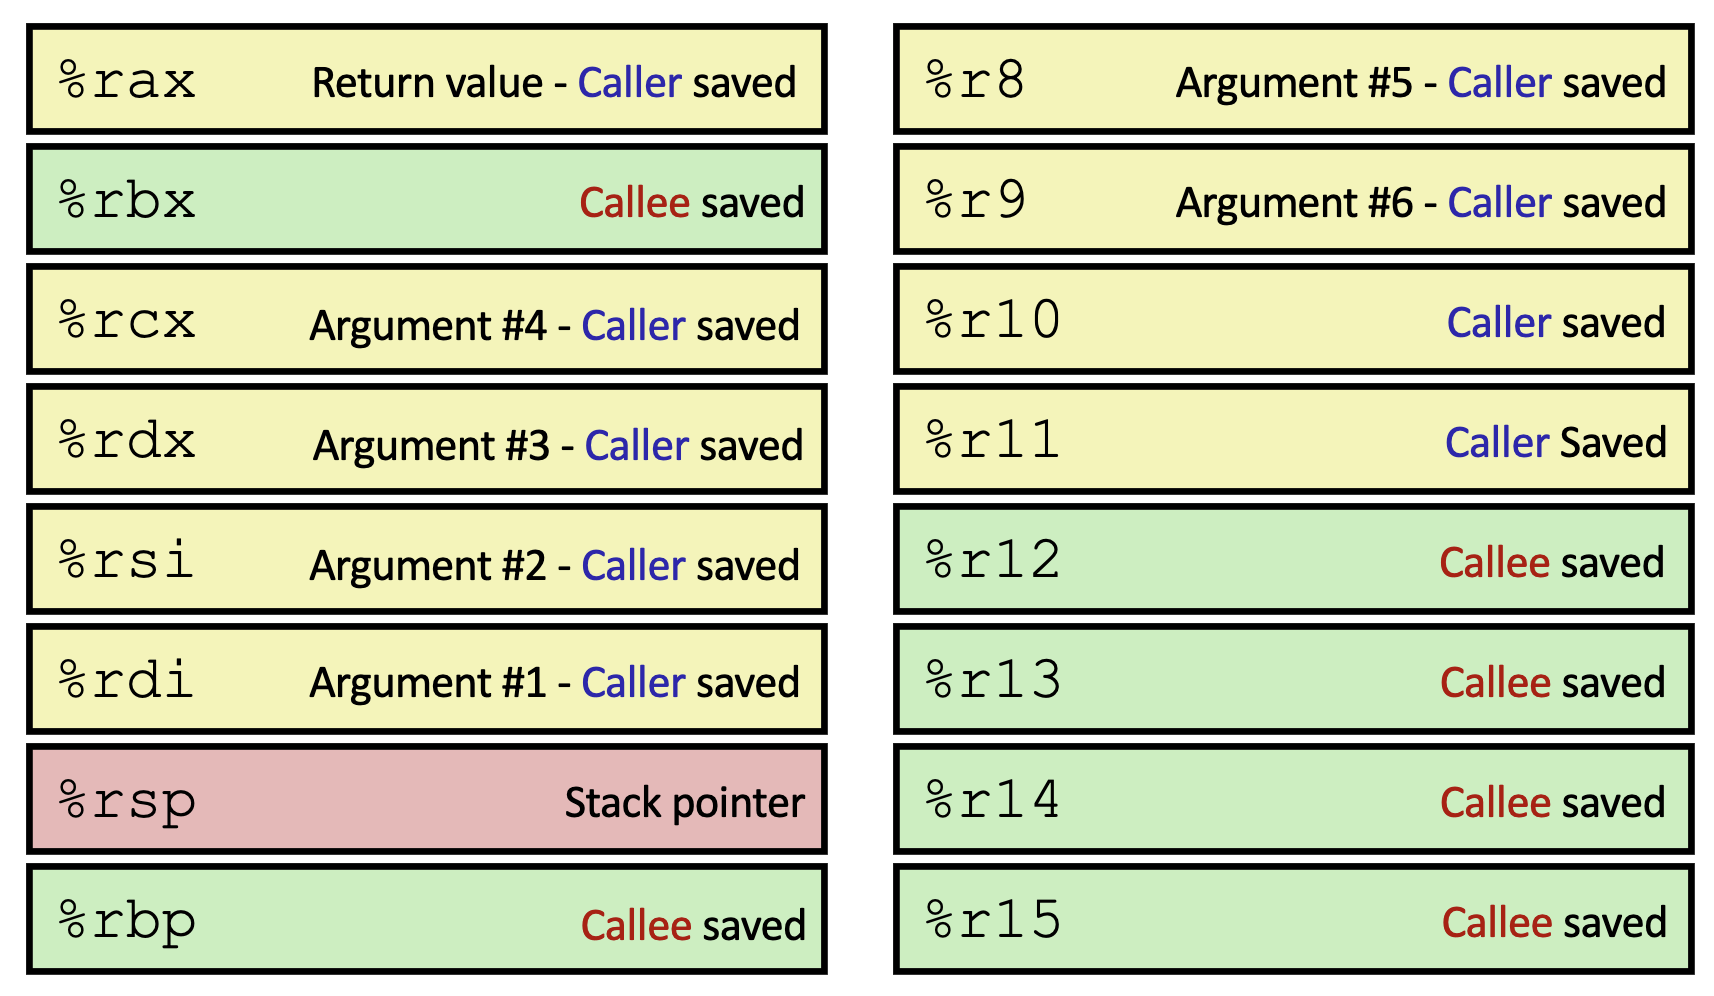
\includegraphics[scale=0.4]{img/caller_callee_save.png}
        \caption{Caller save and callee save registers. } 
        \label{fig:caller_callee_save}
      \end{figure}

      So far, we've traced through simple functions in assembly. In this section, we discuss the interaction between multiple functions in assembly in the context of a larger program. We also introduce some new instructions involved with function management. 

      \begin{definition}[Leave]
        The \textbf{leave} instruction is used to deallocate the current stack frame. For example, the leaveq instruction is a shorthand that the compiler uses to restore the stack and frame pointers as it prepares to leave a function. When the callee function finishes execution, leaveq ensures that the frame pointer is restored to its previous value. It is equivalent to the following two instructions: 
        \begin{align*}
          \texttt{leaveq} && \texttt{movq \%rbp, \%rsp} \\
                          && \texttt{popq \%rbp}
        \end{align*}
      \end{definition}
    
      \begin{definition}[Call and Return]
        The \textbf{call} instruction is used to call a function and the \textbf{ret} to return from a function. The callq and retq instructions play a prominent role in the process where one function calls another. Both instructions modify the instruction pointer (register \%rip). 

        \begin{enumerate}
          \item When the caller function executes the callq instruction, the current value of \%rip is saved on the stack to represent the return address, or the program address at which the caller resumes executing once the callee function finishes. The callq instruction also replaces the value of \%rip with the address of the callee function. 
            \begin{align*}
              \texttt{callq addr <fname>} && \texttt{push \%rip} \\
                                          && \texttt{mov addr, \%rip}
            \end{align*}
          \item The retq instruction restores the value of \%rip to the value saved on the stack, ensuring that the program resumes execution at the program address specified in the caller function. Any value returned by the callee is stored in \%rax or one of its component registers (e.g., \%eax). The retq instruction is usually the last instruction that executes in any function.
            \begin{align*}
              \texttt{retq} && \texttt{pop \%rip} \\
            \end{align*}
        \end{enumerate}
      \end{definition}

      Let's work through an example to solidify our knowledge. 

      \begin{example}[Calling Functions in Assembly]
        Let's take the following code and trace through main. 
        \begin{figure}[H]
          \centering 
          \noindent\begin{minipage}{.25\textwidth}
          \begin{lstlisting}[]{Code}
            #include <stdio.h>

            int assign(void) {
                int y = 40;
                return y;
            }

            int adder(void) {
                int a;
                return a + 2;
            }

            int main(void) {
                int x;
                assign();
                x = adder();
                printf("x is: %d\n", x);
                return 0;
            }
            .
            .
            .
            .
            .
            .
            .
            .
            .
            .
            .
            .
          \end{lstlisting}
          \end{minipage}
          \hfill
          \begin{minipage}{.74\textwidth}
          \begin{lstlisting}[]{Output}
            0000000000400526 <assign>:
              400526:       55                      push   %rbp
              400527:       48 89 e5                mov    %rsp,%rbp
              40052a:       c7 45 fc 28 00 00 00    movl   $0x28,-0x4(%rbp)
              400531:       8b 45 fc                mov    -0x4(%rbp),%eax
              400534:       5d                      pop    %rbp
              400535:       c3                      retq

            0000000000400536 <adder>:
              400536:       55                      push   %rbp
              400537:       48 89 e5                mov    %rsp,%rbp
              40053a:       8b 45 fc                mov    -0x4(%rbp),%eax
              40053d:       83 c0 02                add    $0x2,%eax
              400540:       5d                      pop    %rbp
              400541:       c3                      retq

            0000000000400542 <main>:
              400542:       55                      push   %rbp
              400543:       48 89 e5                mov    %rsp,%rbp
              400546:       48 83 ec 10             sub    $0x10,%rsp
              40054a:       e8 e3 ff ff ff          callq  400526 <assign>
              40054f:       e8 d2 ff ff ff          callq  400536 <adder>
              400554:       89 45 fc                mov    %eax,-0x4(%rbp)
              400557:       8b 45 fc                mov    -0x4(%rbp),%eax
              40055a:       89 c6                   mov    %eax,%esi
              40055c:       bf 04 06 40 00          mov    $0x400604,%edi
              400561:       b8 00 00 00 00          mov    $0x0,%eax
              400566:       e8 95 fe ff ff          callq  400400 <printf@plt>
              40056b:       b8 00 00 00 00          mov    $0x0,%eax
              400570:       c9                      leaveq
              400571:       c3                      retq
          \end{lstlisting}
          \end{minipage}
          \caption{C code and its assembly equivalent. Main function calls two other functions. } 
          \label{fig:calling_functions}
        \end{figure}

        Let's trace through what happens here in detail. This will be long. 

        \begin{enumerate}
          \item \texttt{\%rbp} is the base pointer that is initialized to something. Before we even begin main, say that we have the following initializations, where \texttt{\%eax}, \texttt{\%edi} is garbage. \texttt{\%rsp} denotes where on the stack we are right before calling to main, \textbf{\%rbp} is the base pointer to the current program, and \textbf{\%rip} should be the address of the first instruction in main. Again since we work with integers we use the lower 32-bits of the registers. \texttt{\%rip} now points to the next instruction. 
            \begin{center}
              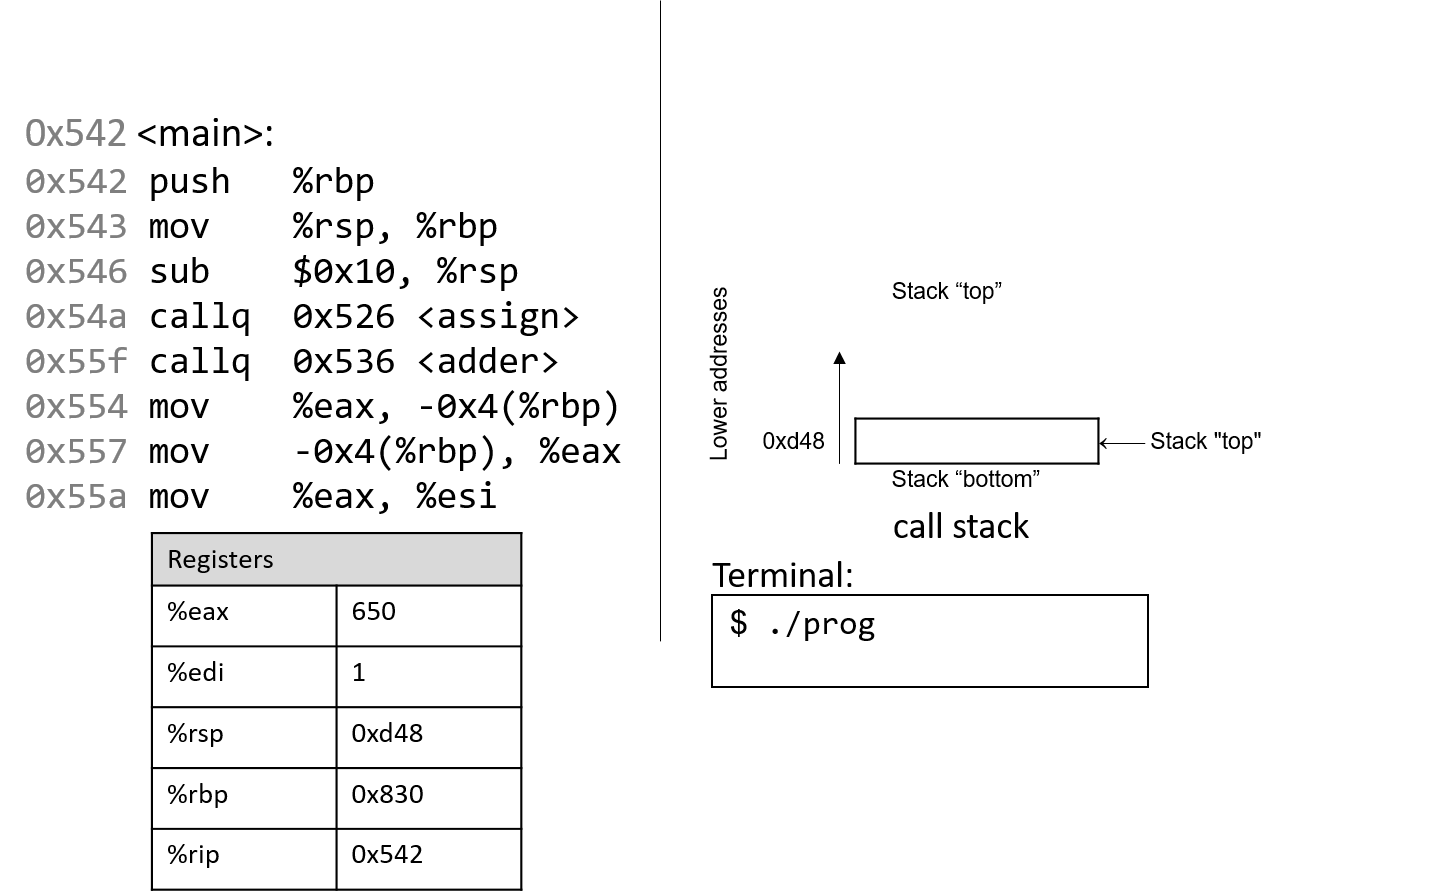
\includegraphics[scale=0.5]{img/Slide1.png}
            \end{center}  

          \item Now we start the main function. By calling main, the base pointer \texttt{\%rbp} of the stack outside of the main frame will be overwritten by the base of the main stack frame, so we must save it for when main is done. Therefore, we push it onto the stack where \texttt{\%rsp} is pointing. \texttt{\%rip} now points to the next instruction. 
            \begin{center}
              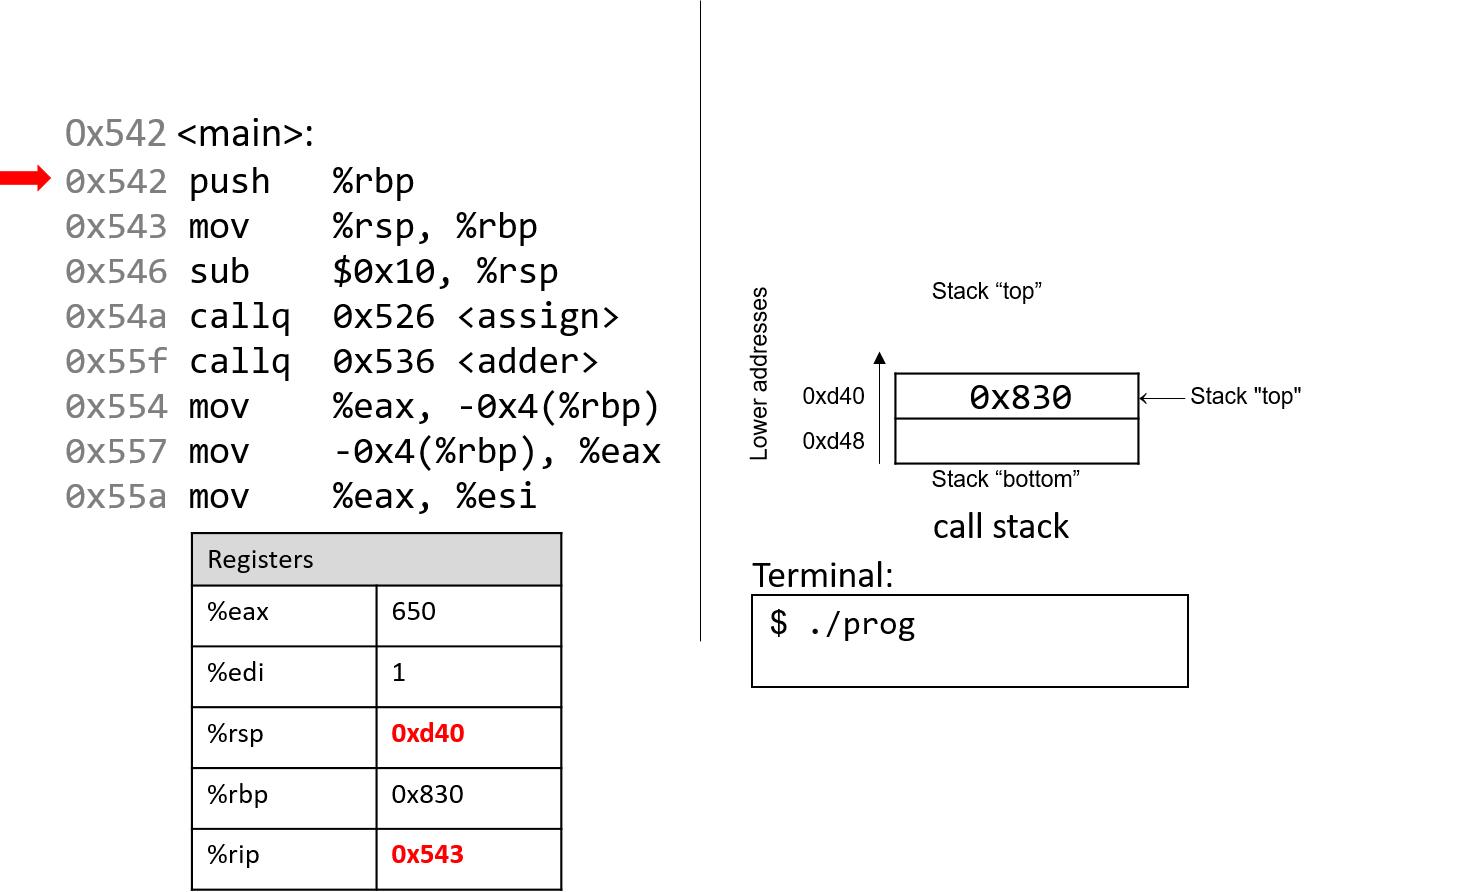
\includegraphics[scale=0.5]{img/Slide2.png}
            \end{center}

          \item Then we actually change the location of the base pointer to the top of the stack, which now includes the first instruction in main. 
            \begin{center}
              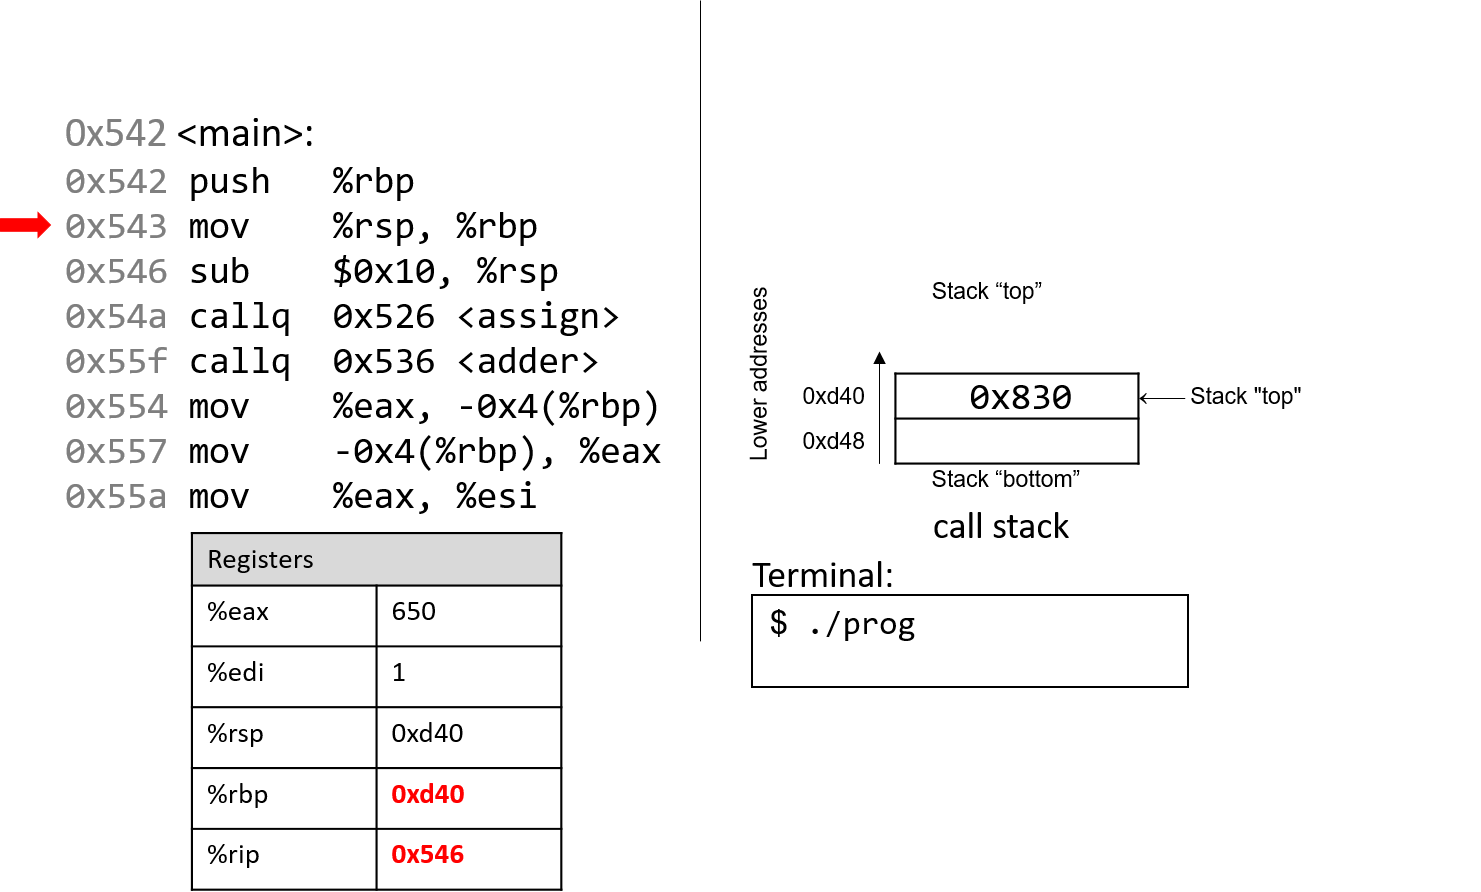
\includegraphics[scale=0.5]{img/Slide3.png}
            \end{center} 

          \item Now we manually change the stack pointer and have it grow by two bytes (\texttt{0x10}). Therefore, \texttt{\%rsp} is decremented by \texttt{0x10} and \texttt{\%rip} points to the next instruction at \texttt{0x54a}. 
            \begin{center}
              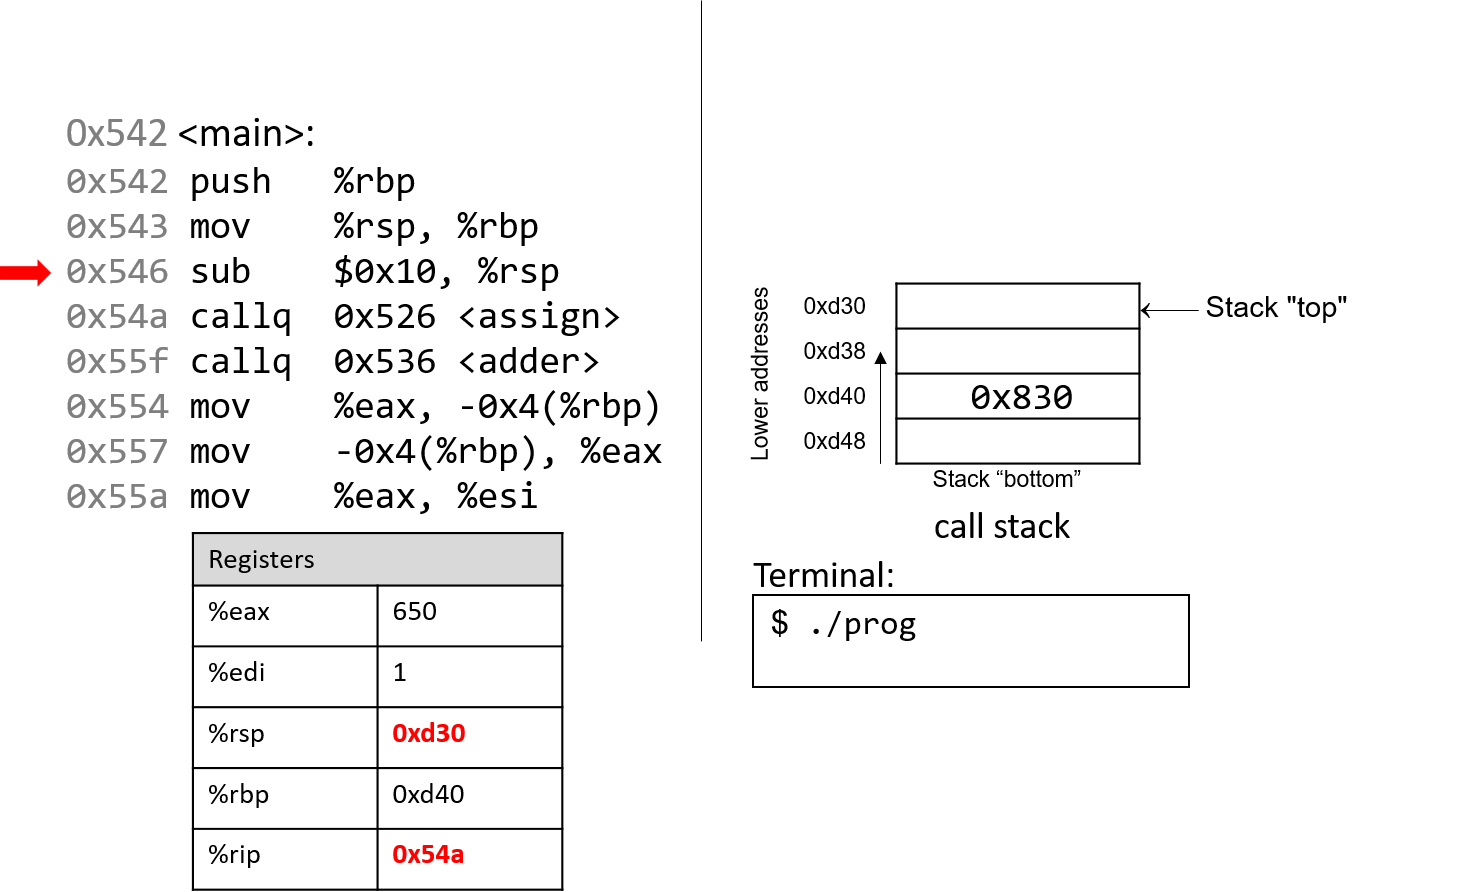
\includegraphics[scale=0.5]{img/Slide4.png}
            \end{center}
            
          \item Now the next instruction pointed at by \texttt{\%rip} is the \texttt{callq} instruction, which tells to go to the address of the \texttt{assign} function. We by default first update \texttt{\%rip} to point to the next instruction at \texttt{0x55f}. However, this should not be the actual next instruction that we execute since we are calling another function. Rather, we want to update \texttt{\%rip} to address \texttt{0x526} where \texttt{assign} is located at, but after completion we also want to know that we want to execute the instruction after it at address \texttt{0x55f}. Therefore, we should \textit{save} address \texttt{0x55f} onto the stack and then update \texttt{\%rip} to point to \texttt{0x526}. This is what we refer to as a \textbf{return address}. 
            \begin{center}
              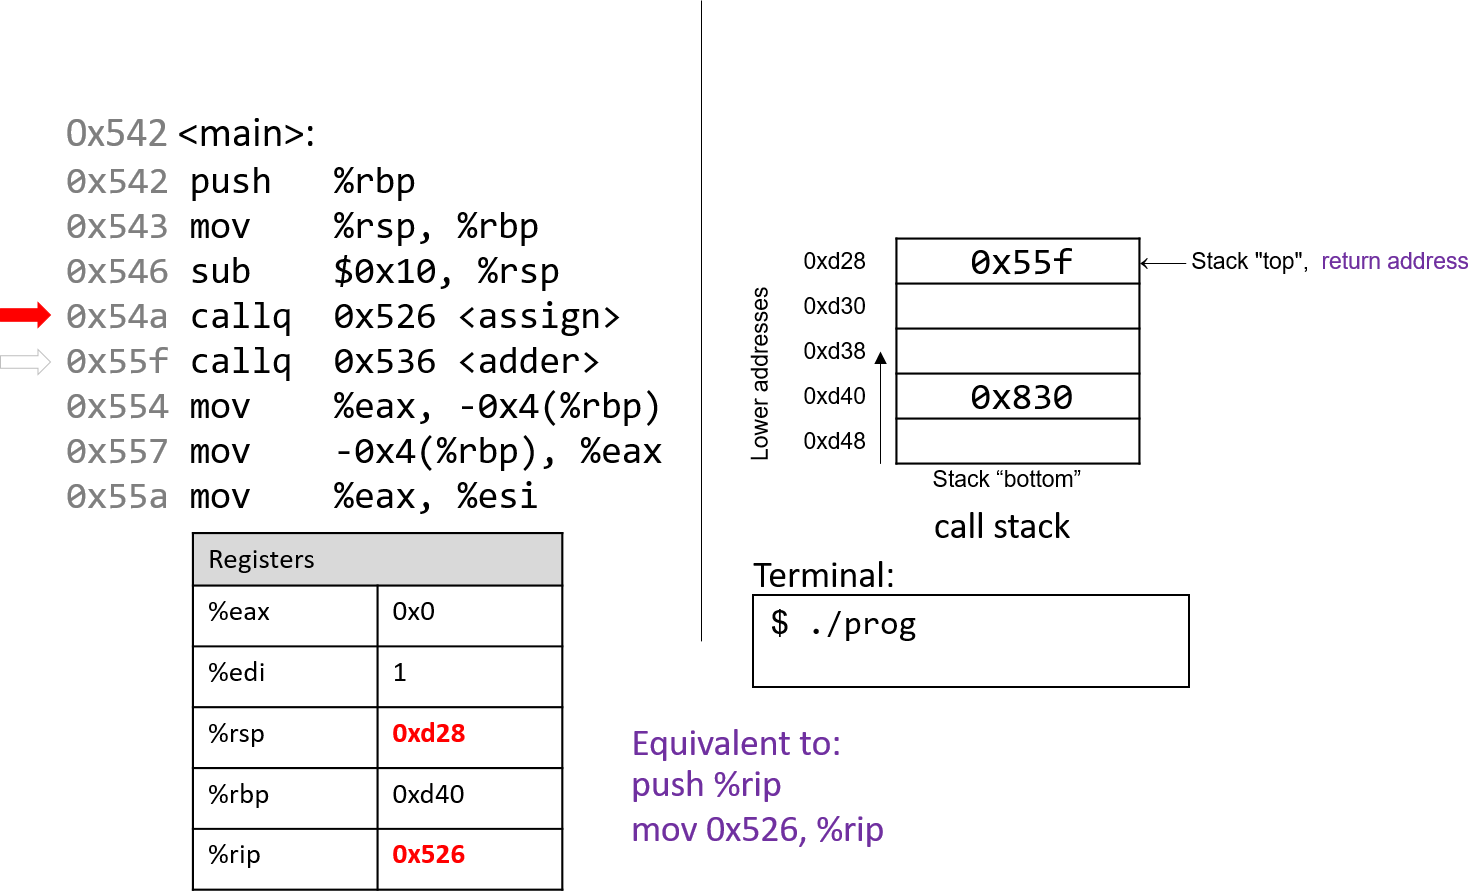
\includegraphics[scale=0.5]{img/Slide5.png}
            \end{center}

          \item \texttt{\%rip} is incremented to the next address. We step into the \texttt{assign} function, which is now a new stack frame, so the first thing we do is save the base pointer of the main stack frame onto the stack since we must immediately update it with the base pointer of the assign stack frame, which is where \texttt{\%rsp} is pointing to. 
            \begin{center}
              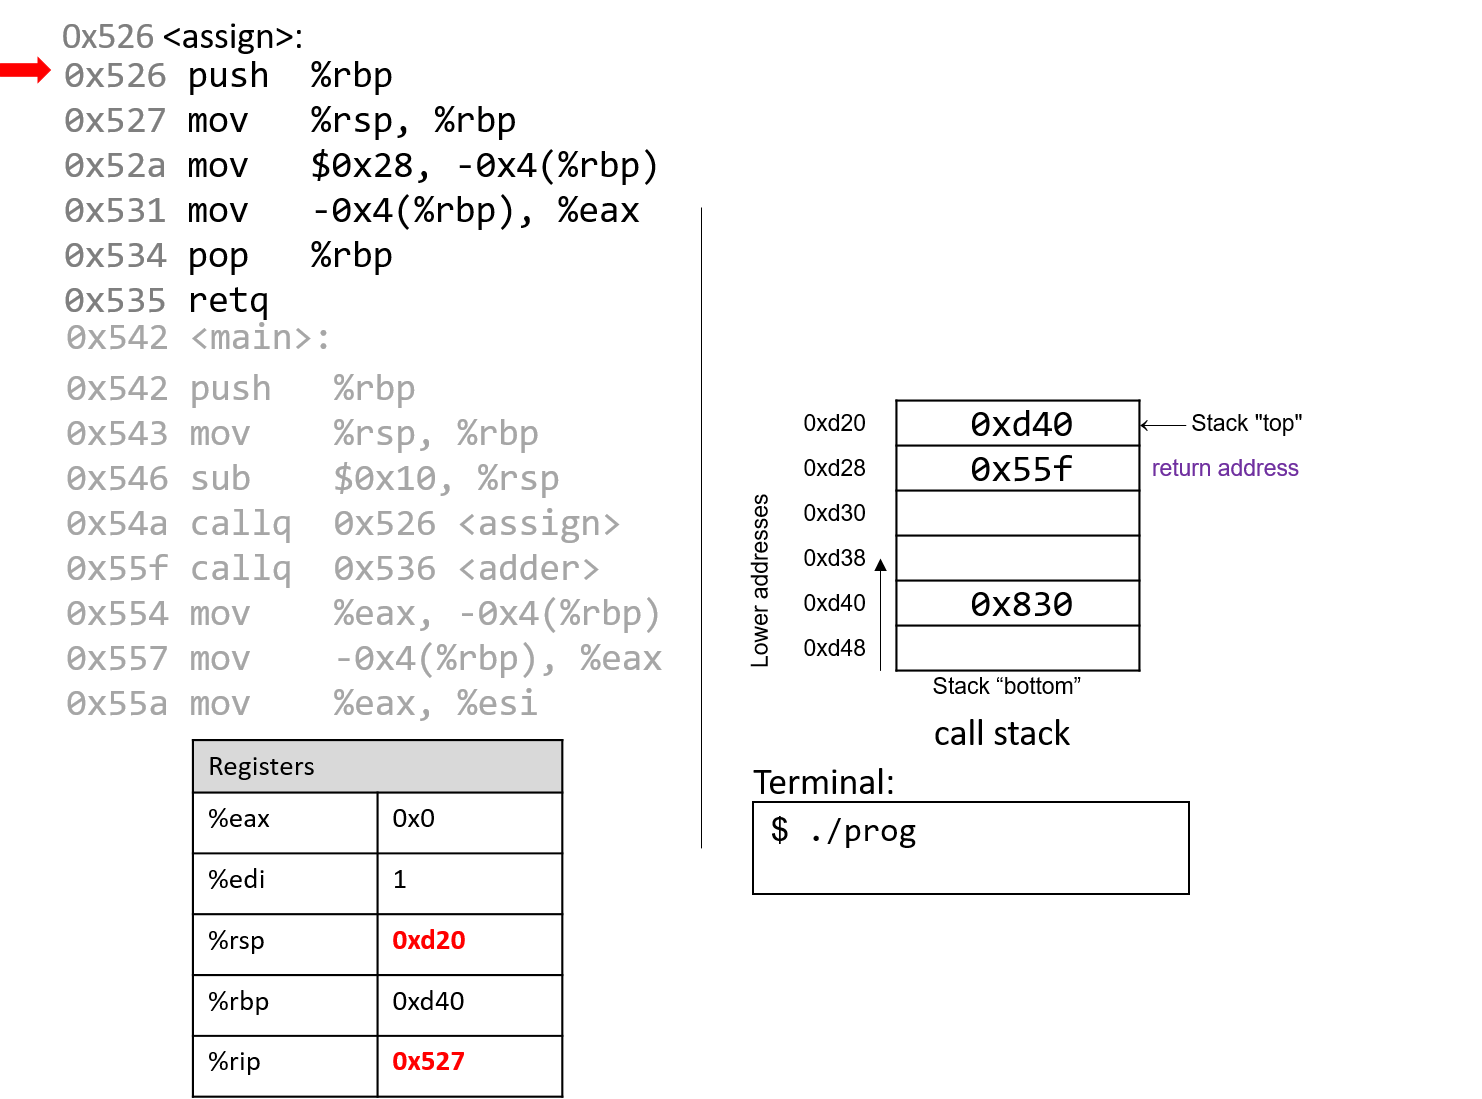
\includegraphics[scale=0.5]{img/Slide6.png}
            \end{center}

          \item \texttt{\%rip} is incremented to the next address. We then update the base pointer to the top of the stack. 
            \begin{center}
              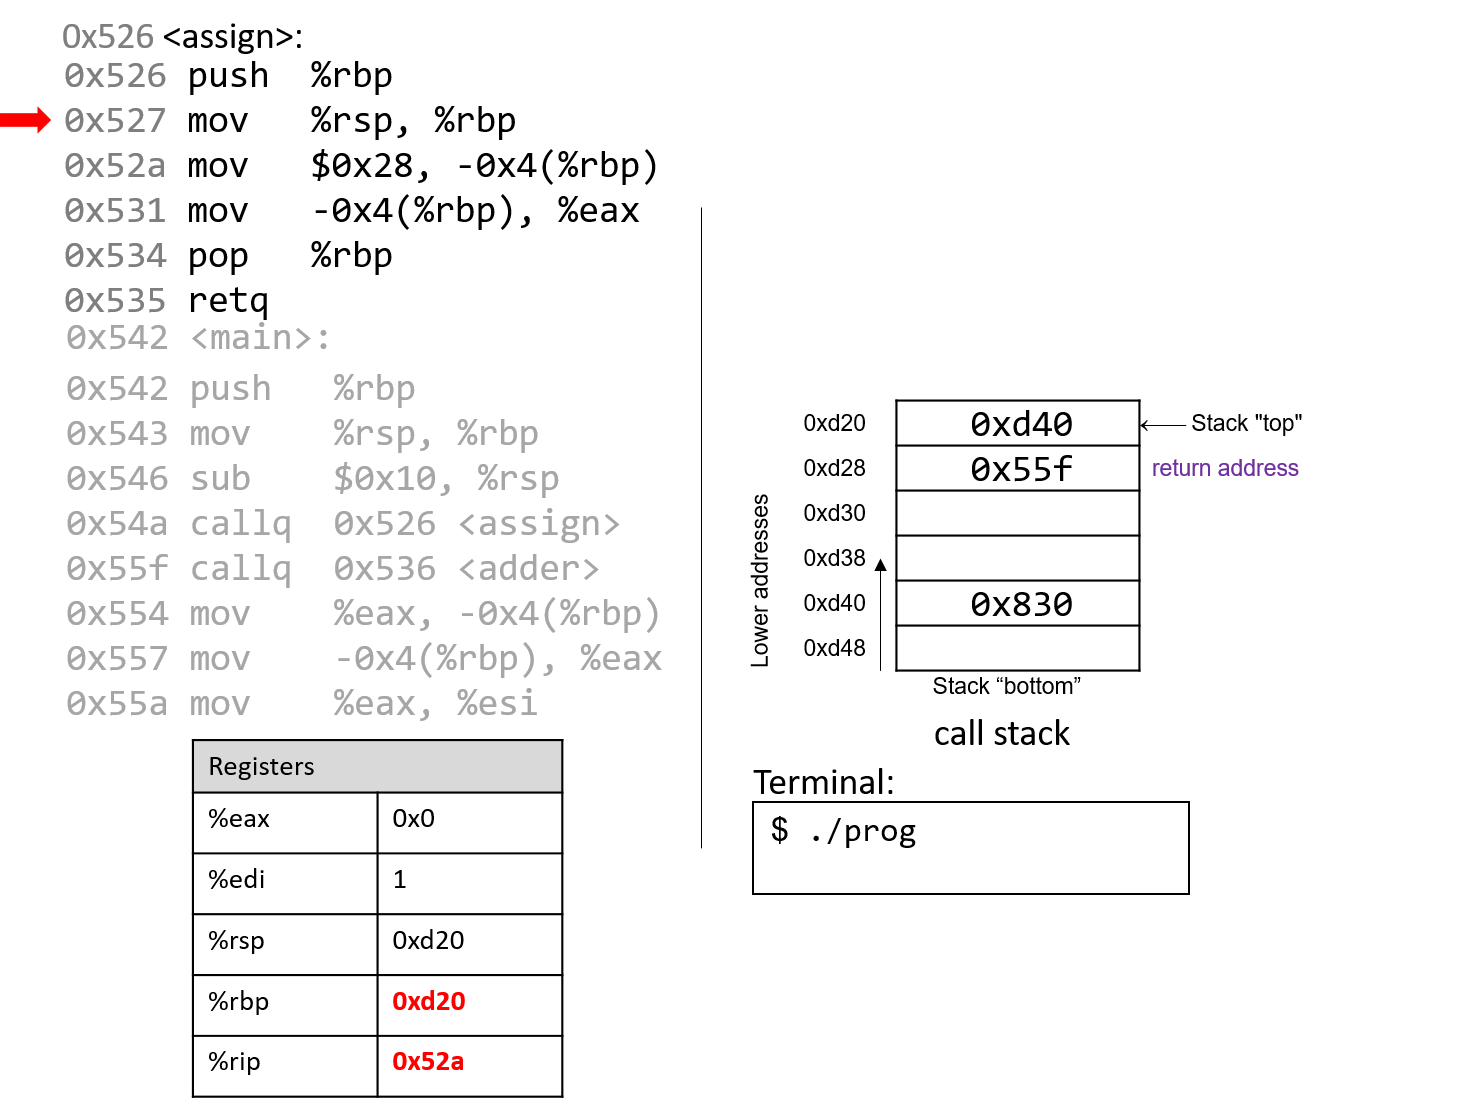
\includegraphics[scale=0.5]{img/Slide7.png}
            \end{center}

          \item Now we want to move the number \texttt{0x28} (40) into the memory location \texttt{-0x4(\%rbp)} of the stack, which is 4 bytes above the frame pointer, which is also the stack pointer. It is common that the frame pointer is used to reference locations on the stack. Note that this does not update the stack pointer.  
            \begin{center}
              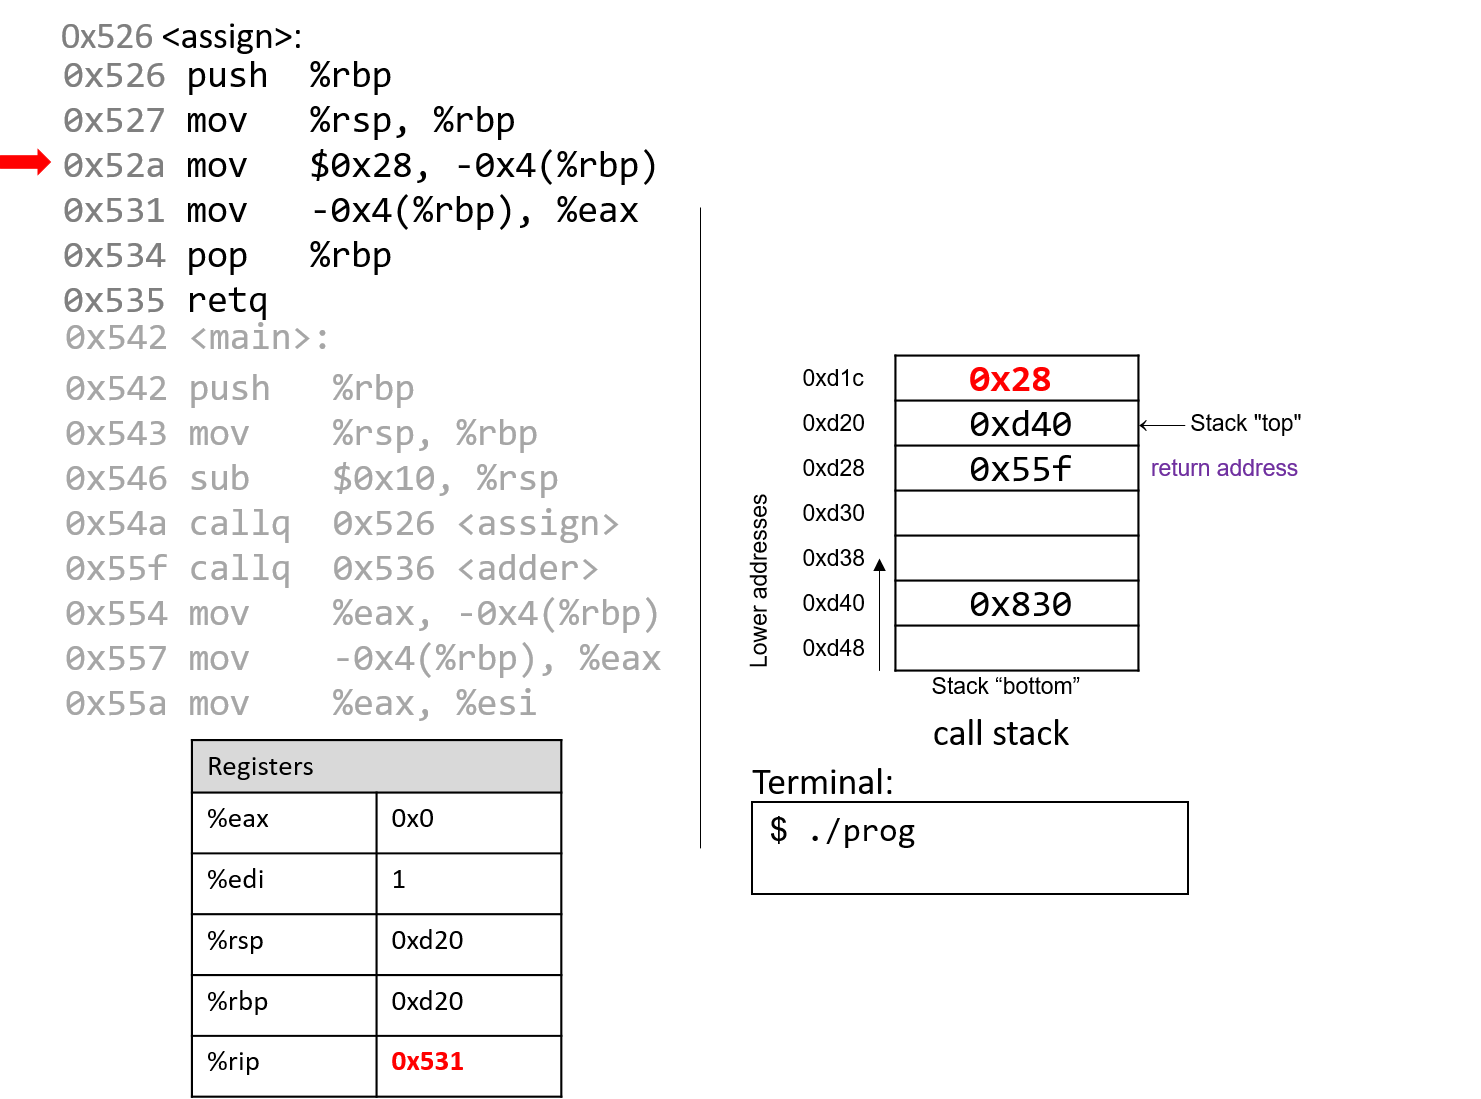
\includegraphics[scale=0.5]{img/Slide8.png}
            \end{center}

          \item Now we take the same address where we stored \texttt{0x28} to and move it into \texttt{\%eax}, effectively loading 40 onto the return value. 
            \begin{center}
              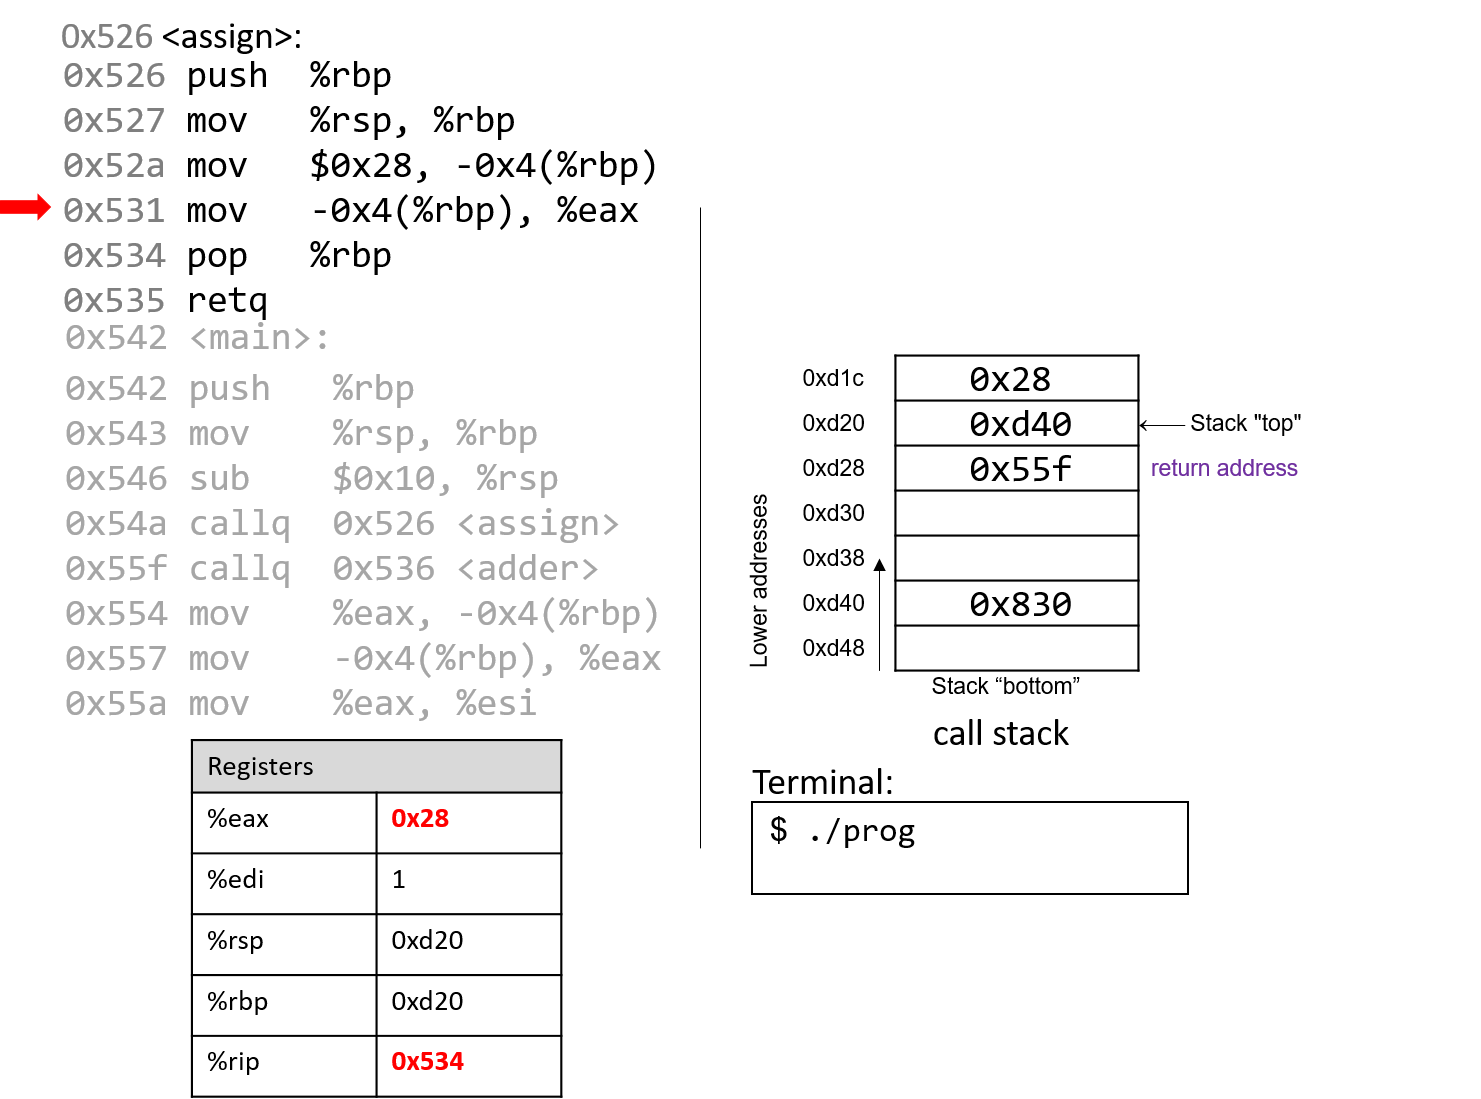
\includegraphics[scale=0.5]{img/Slide9.png}
            \end{center}

          \item We see that we will return this value soon, but before we do, we want to make sure that when the assign stack frame gets deleted (not really, but overwritten), we want to restore the base pointer of the main stack frame. We have already saved this before at \texttt{\%rsp}, which hasn't changed since we only worked with displacements from the base pointer. We retrieve the main stack pointer data and load it back into \texttt{\%rbp}. Note that this increments \texttt{\%rsp} by 8 bytes, shrinking the stack, and we are technically out of the assign stack frame. 
            \begin{center}
              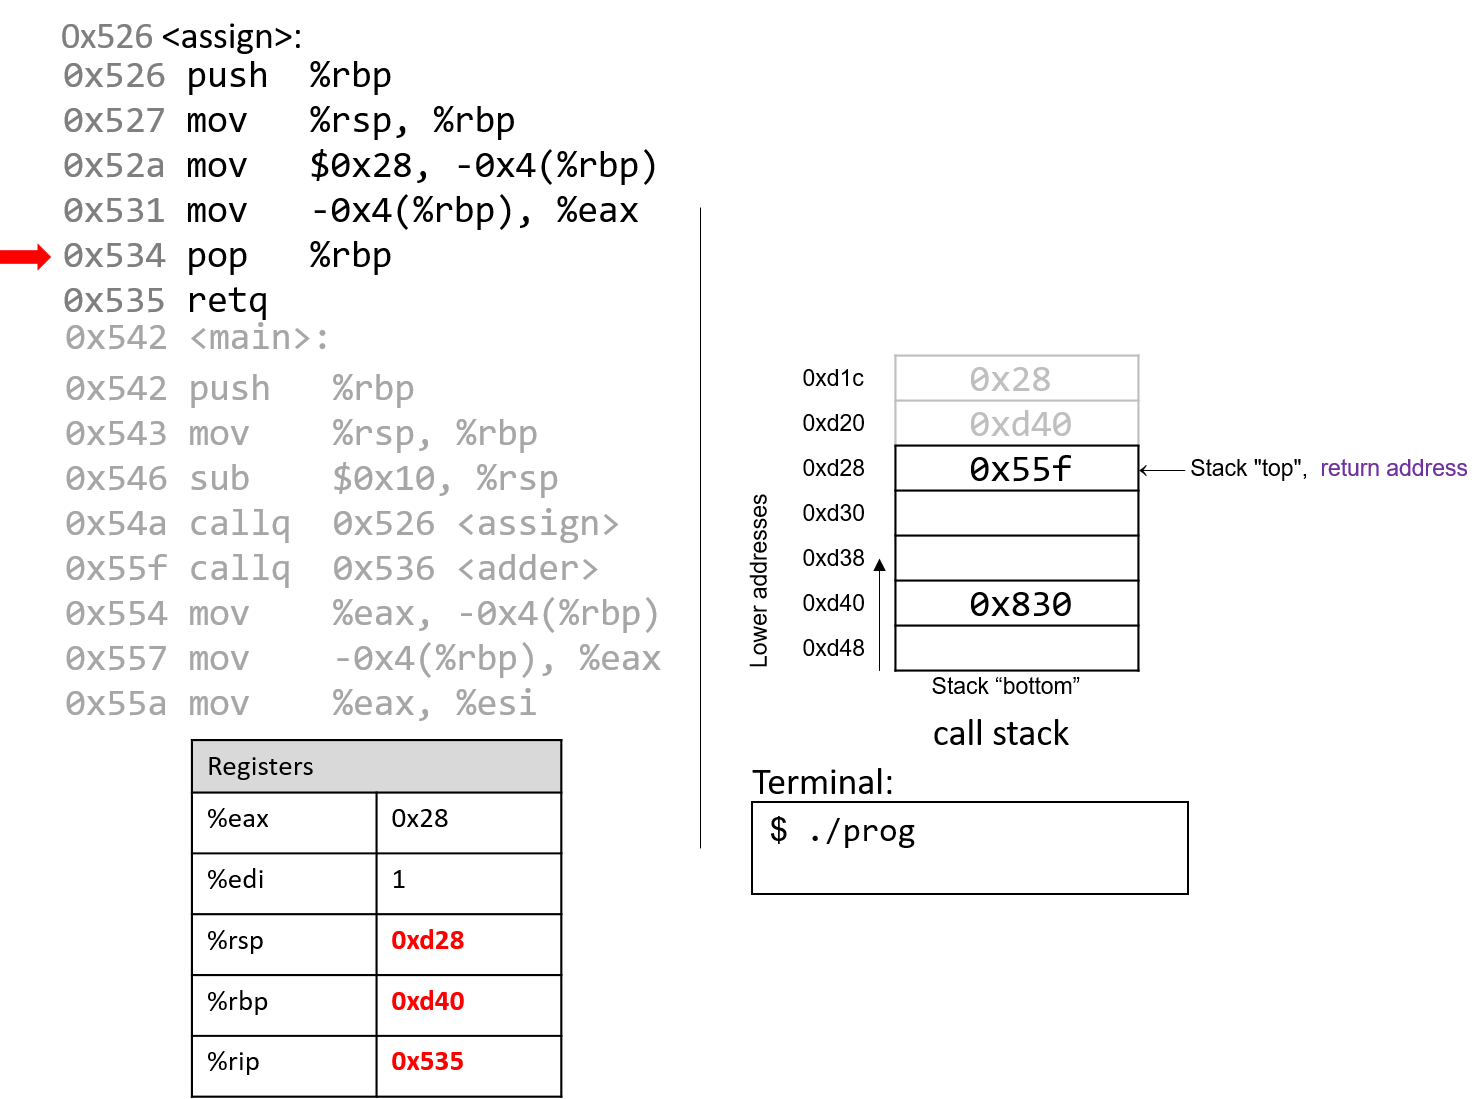
\includegraphics[scale=0.5]{img/Slide10.png}
            \end{center} 

          \item Note that at this point, since \texttt{\%rbp} was popped off, the next value that is at the top of the stack is the address \texttt{\%rip} that we store earlier, which points to the next execution in main. When \texttt{retq} executes, this value at the top of the stack is popped into \texttt{\%rip}, allowing main to continue executing within the main stack frame. Note that the return value is stored in \texttt{\%eax}.
            \begin{center}
              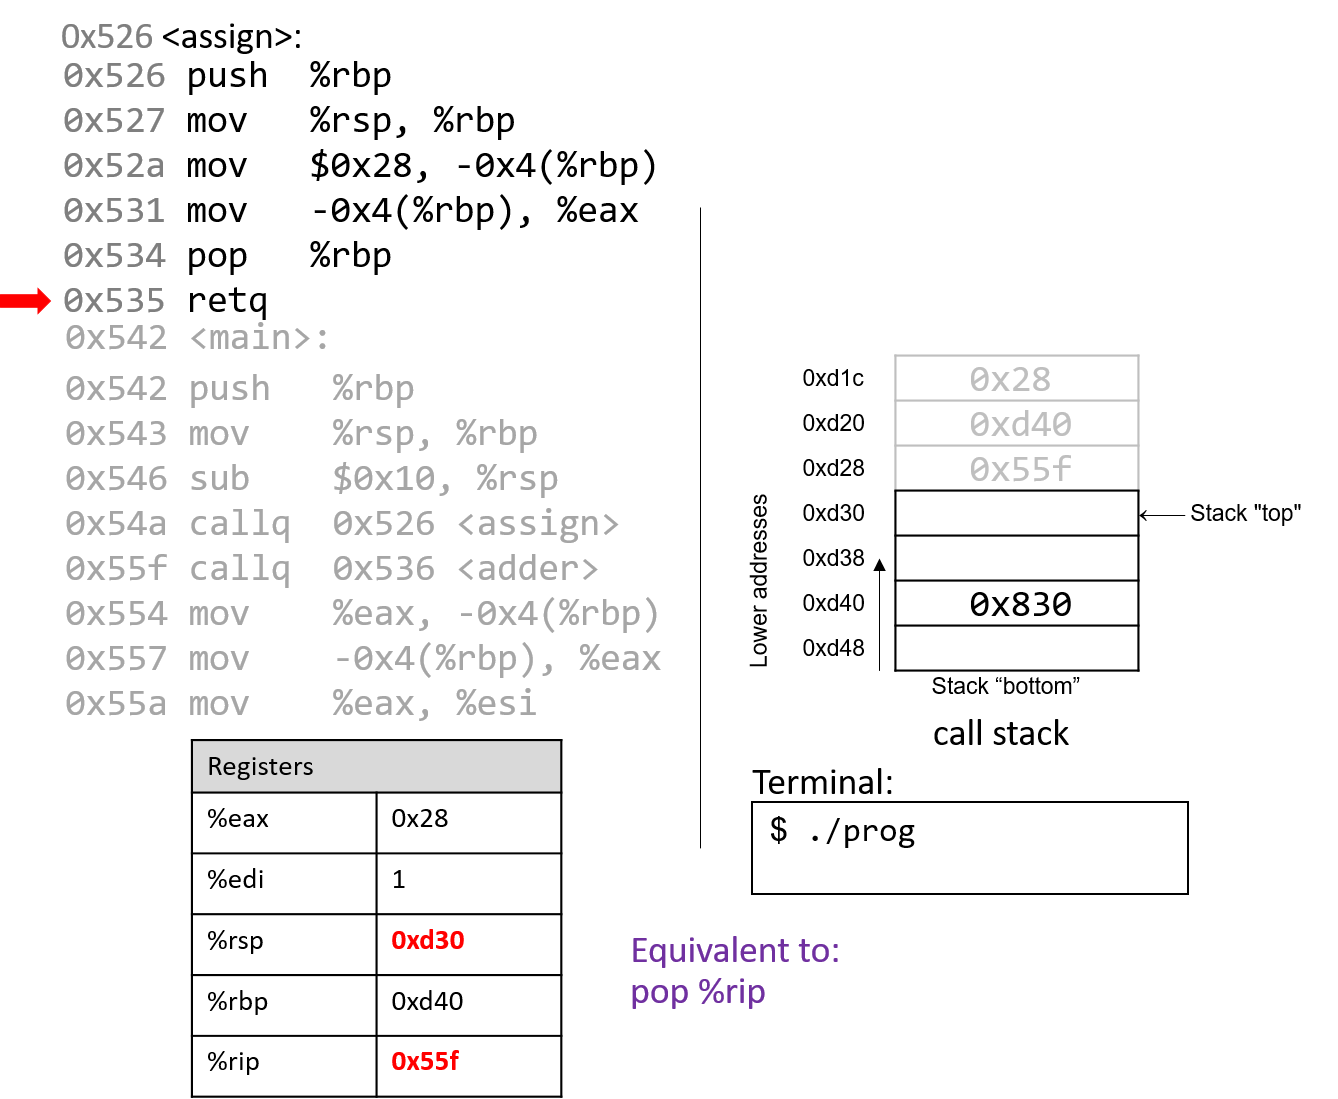
\includegraphics[scale=0.5]{img/Slide11.png}
            \end{center}

          \item Now we execute the next instruction in \texttt{\%rip} which is a call to the \texttt{adder} function. \texttt{\%rip} is automatically updated to the next address at \texttt{0x554}, but since this is a \texttt{callq} instruction, we first want to store this \texttt{\%rip} into the stack so we can come back to it, and then update \texttt{\%rip} to the first instruction in \texttt{adder}, which is address \texttt{0x536}. 
            \begin{center}
              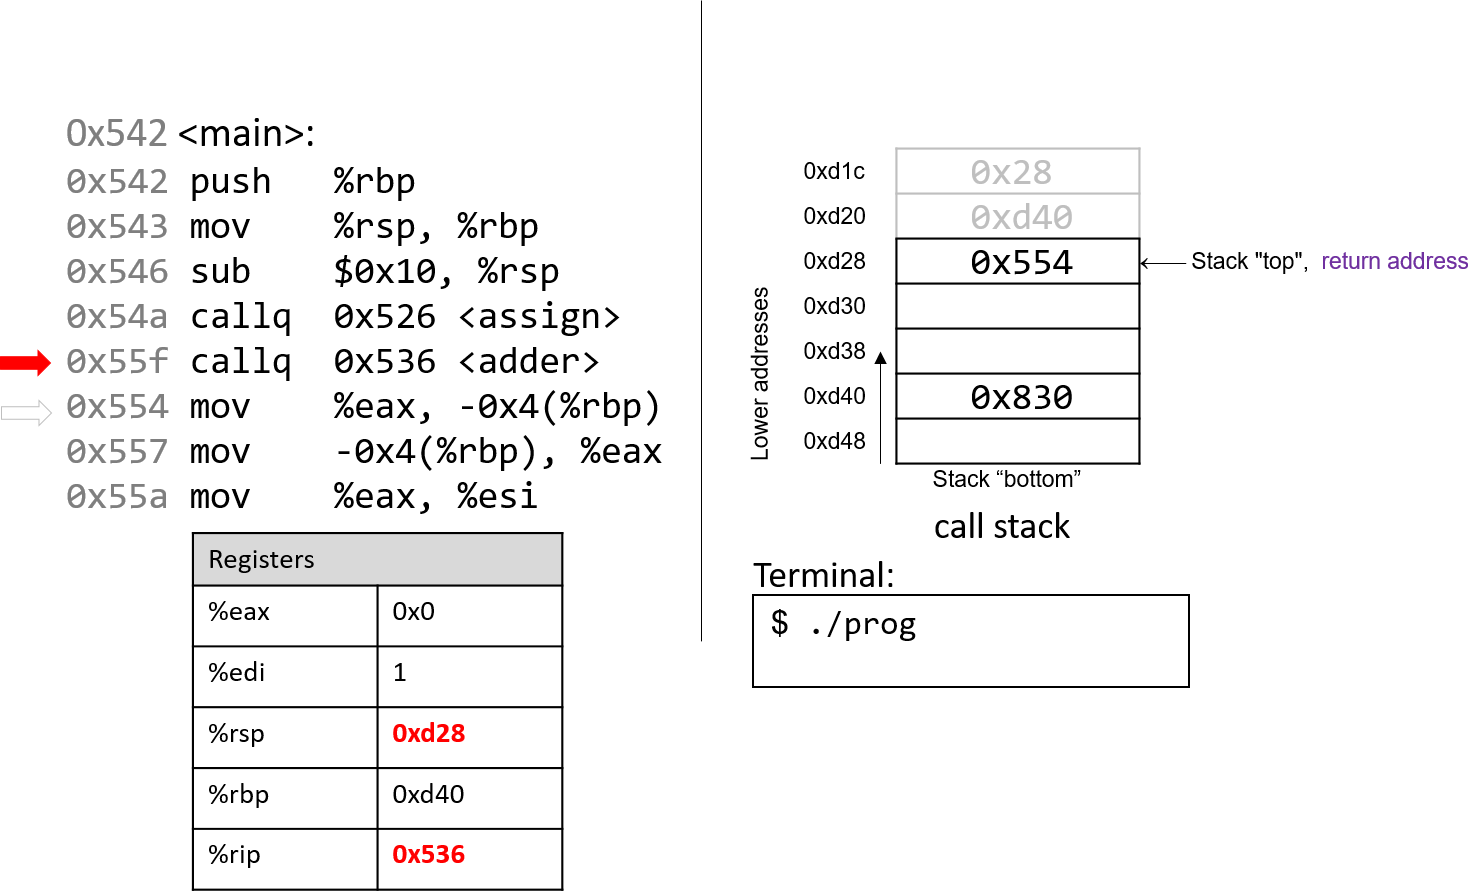
\includegraphics[scale=0.5]{img/Slide12.png}
            \end{center}

          \item Since we are in the adder function, this creates a new stack frame and we must update \texttt{\%rbp}. Again, we don't want to overwrite the base pointer of main, so we save it onto the stack by pushing \texttt{\%rbp}. 
            \begin{center}
              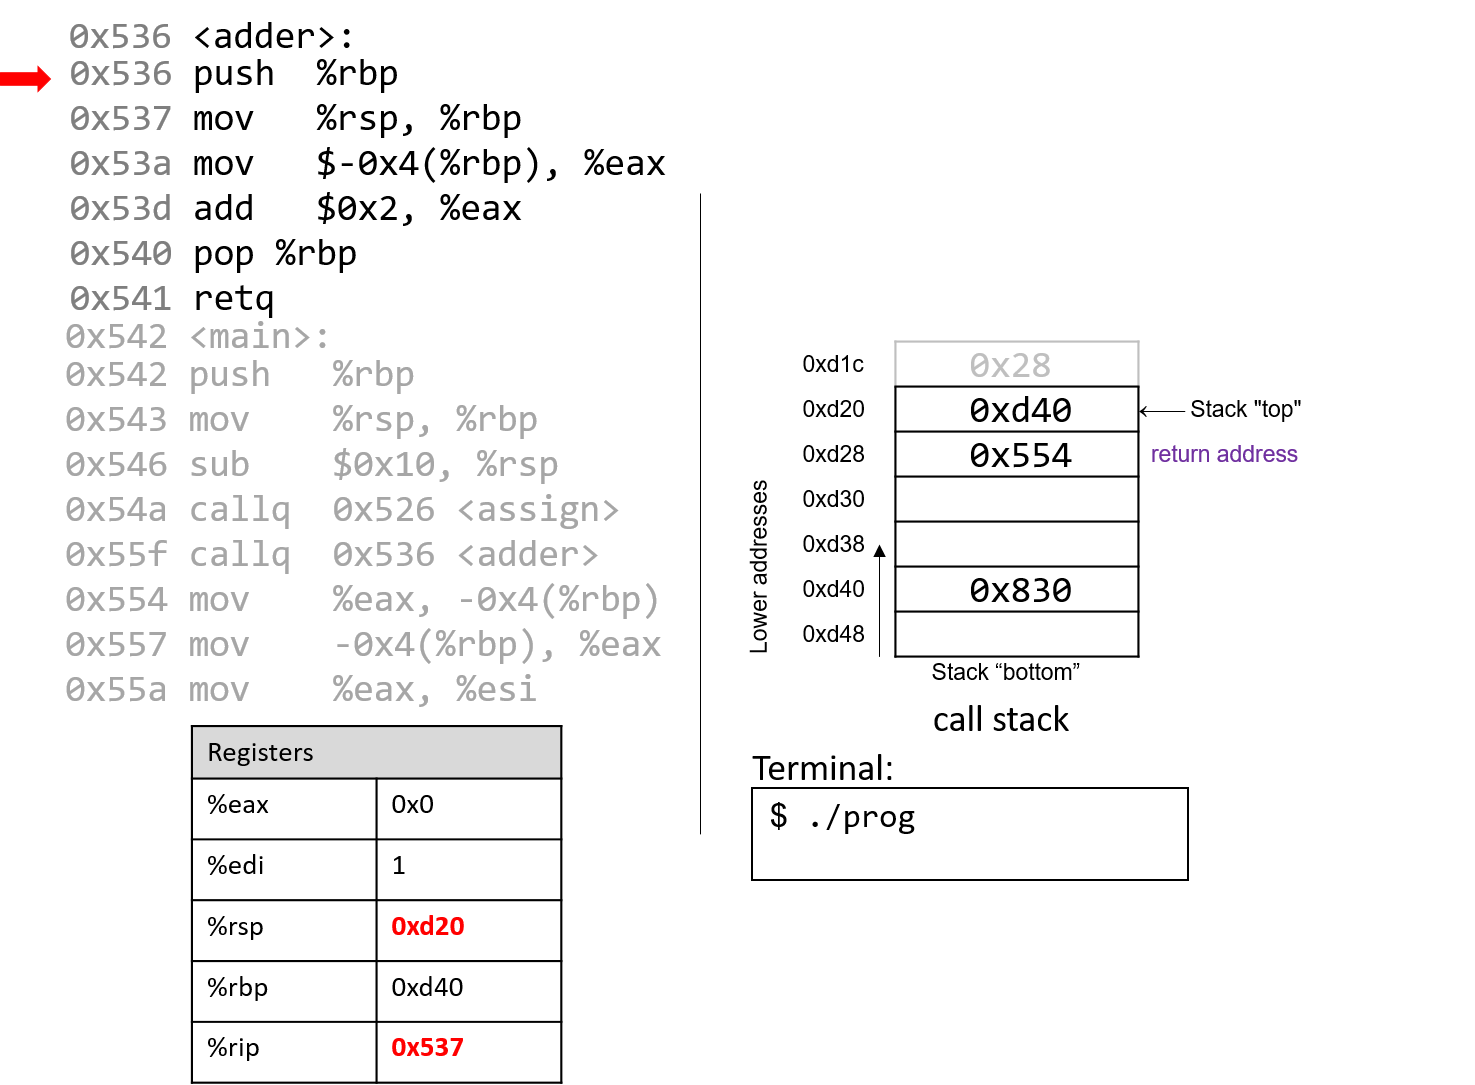
\includegraphics[scale=0.5]{img/Slide13.png}
            \end{center}

          \item Then we update \texttt{\%rbp} to the current stack pointer. 
            \begin{center}
              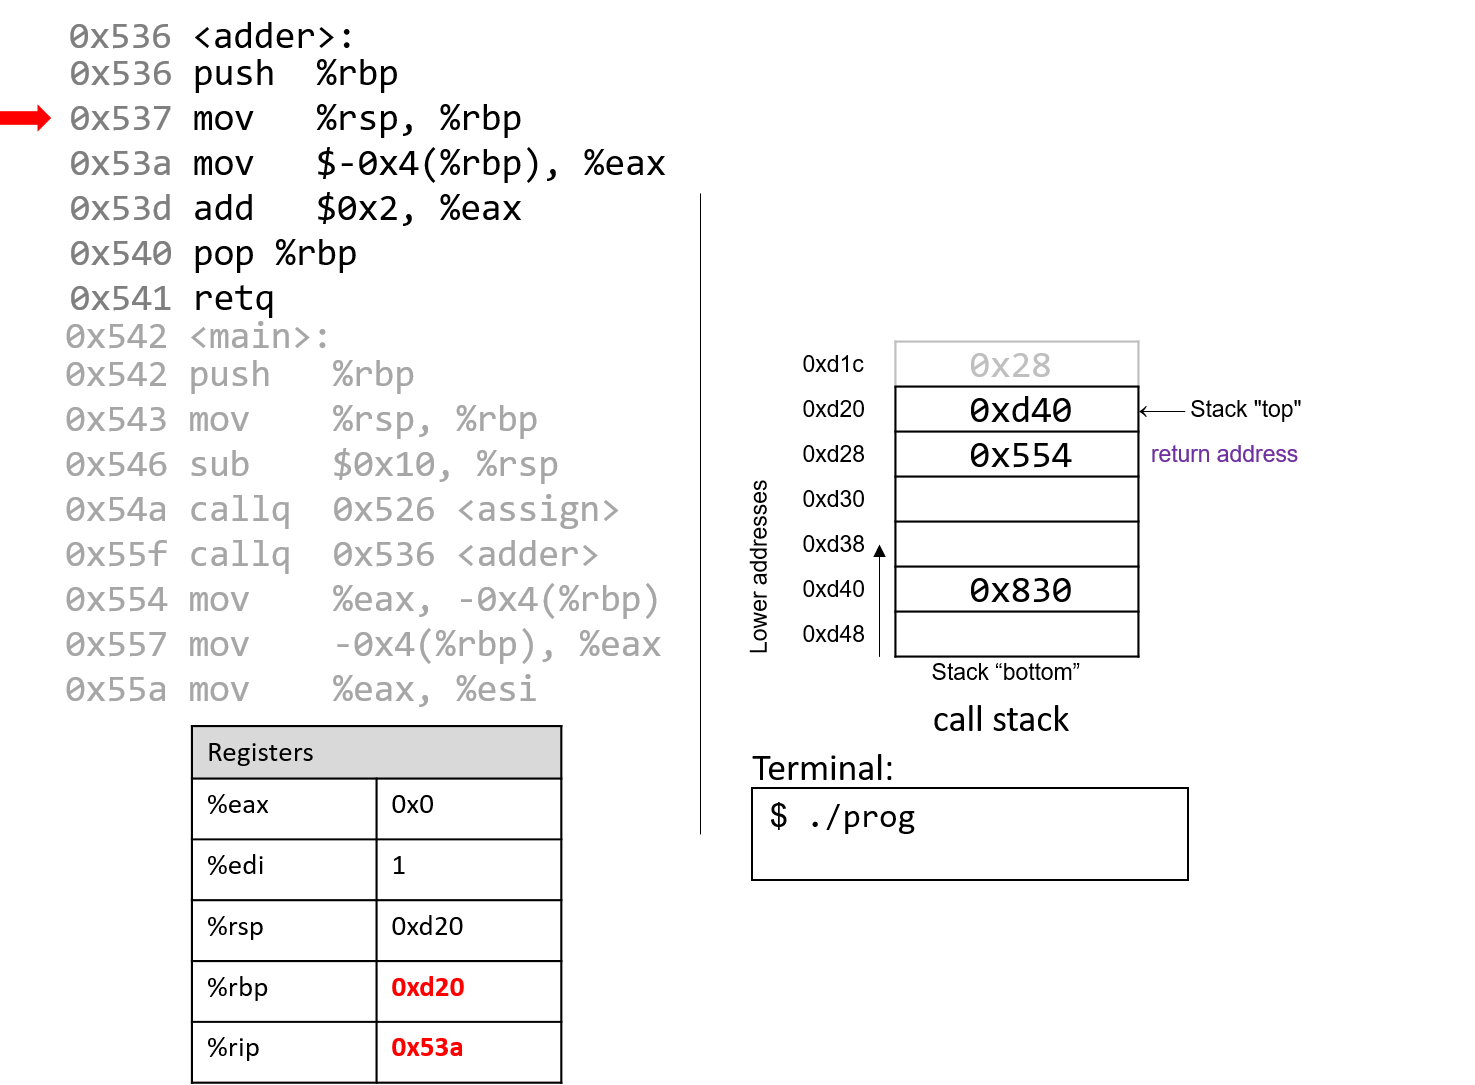
\includegraphics[scale=0.5]{img/Slide14.png}
            \end{center}

          \item This part is a bit tricky. Note that the value of \texttt{0x28} still lives at \texttt{0xd1c}, which is conveniently at address \texttt{-0x4(\%rbp)}. Therefore, when we call \texttt{int a;} in that corresponding line in \texttt{adder}, we can actually add 2 to it, though it seems like there was no value assigned to it. This is just a trick though. So, we can take these remnant value and store it into \texttt{\%eax}. 
            \begin{center}
              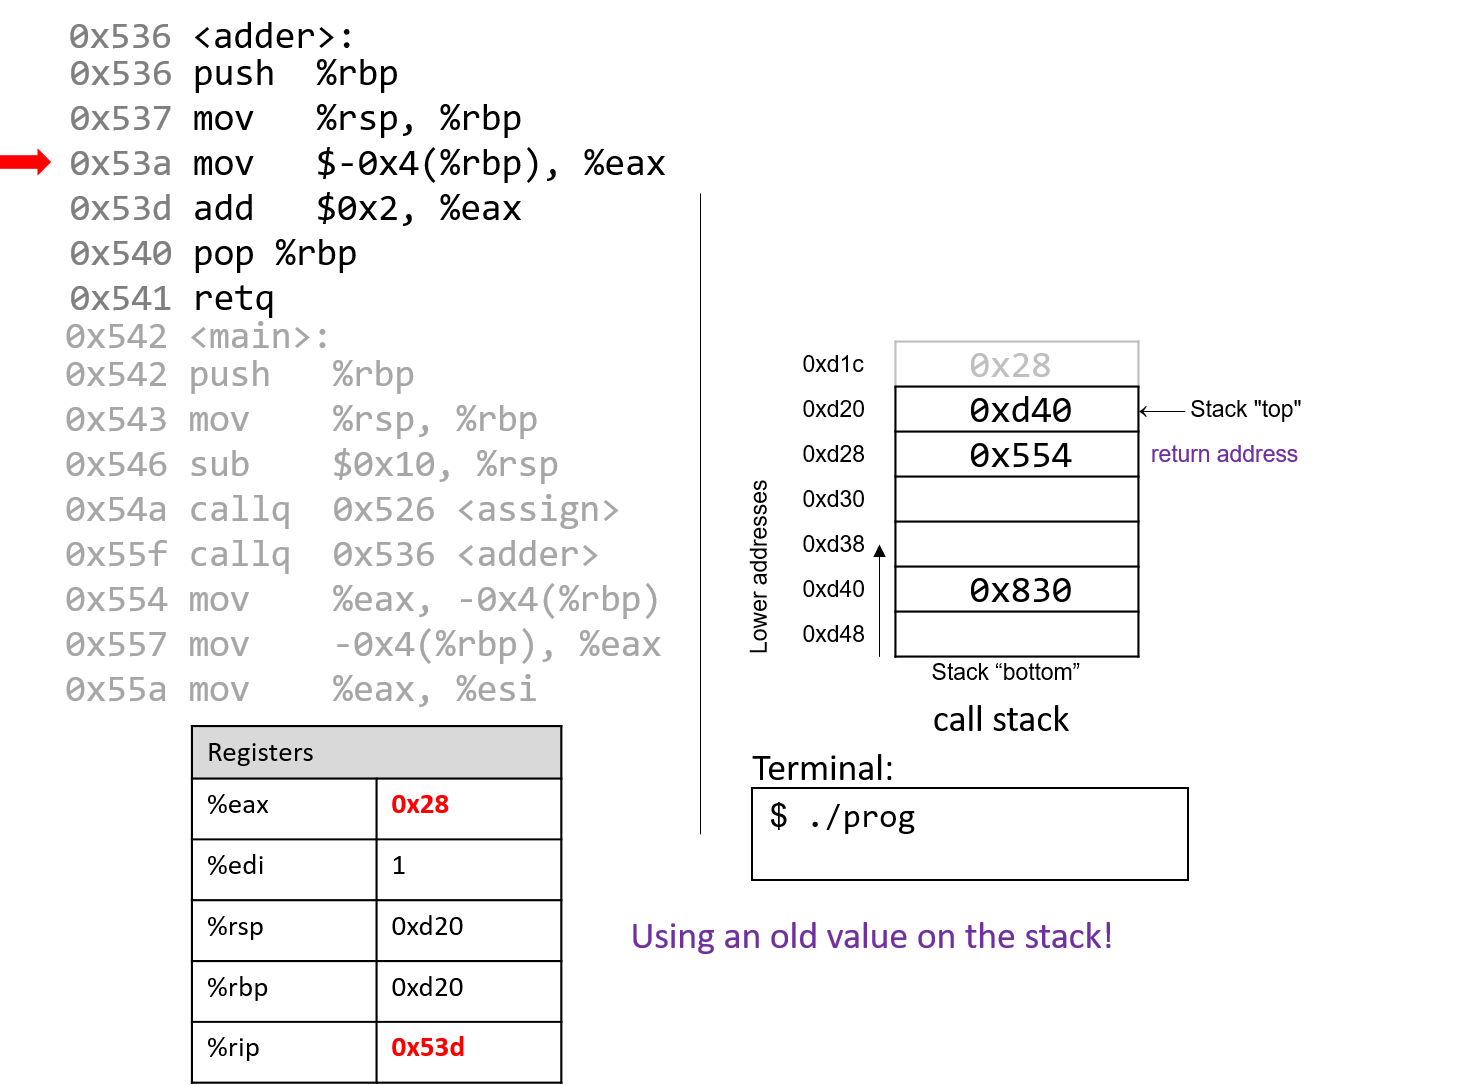
\includegraphics[scale=0.5]{img/Slide15.png}
            \end{center}

          \item We then add 2 to it. 
            \begin{center}
              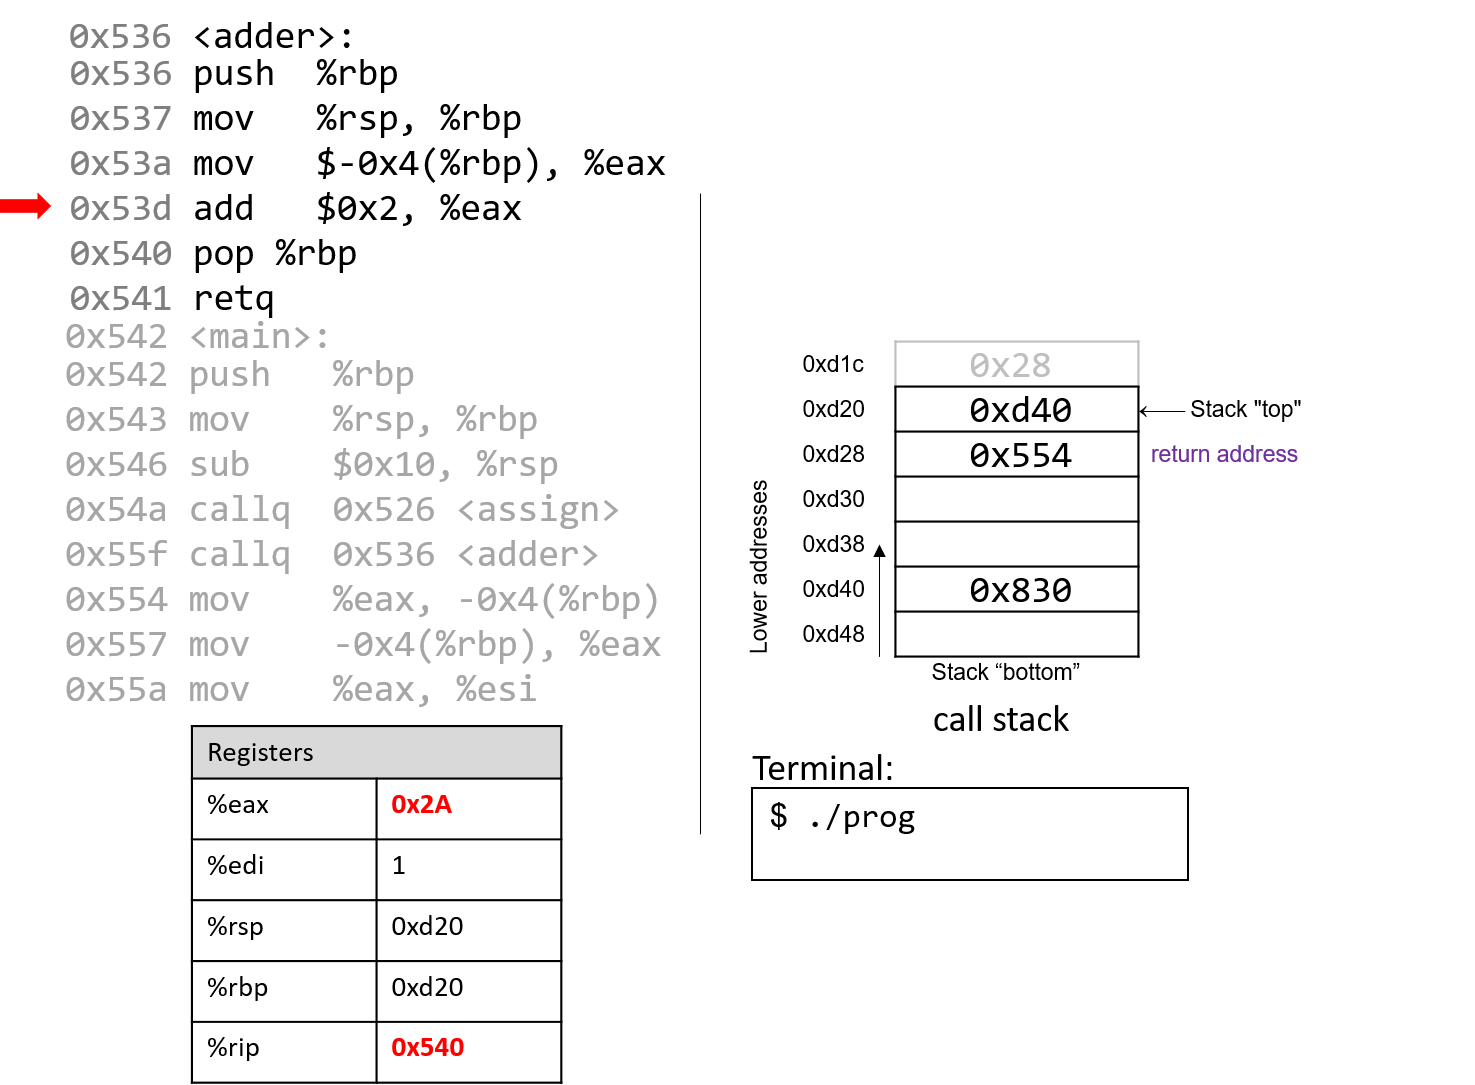
\includegraphics[scale=0.5]{img/Slide16.png}
            \end{center}

          \item Now we are almost done, so we pop the base pointer of the main stack frame, at \texttt{0xd40}, back into \texttt{\%rbp}. 
            \begin{center}
              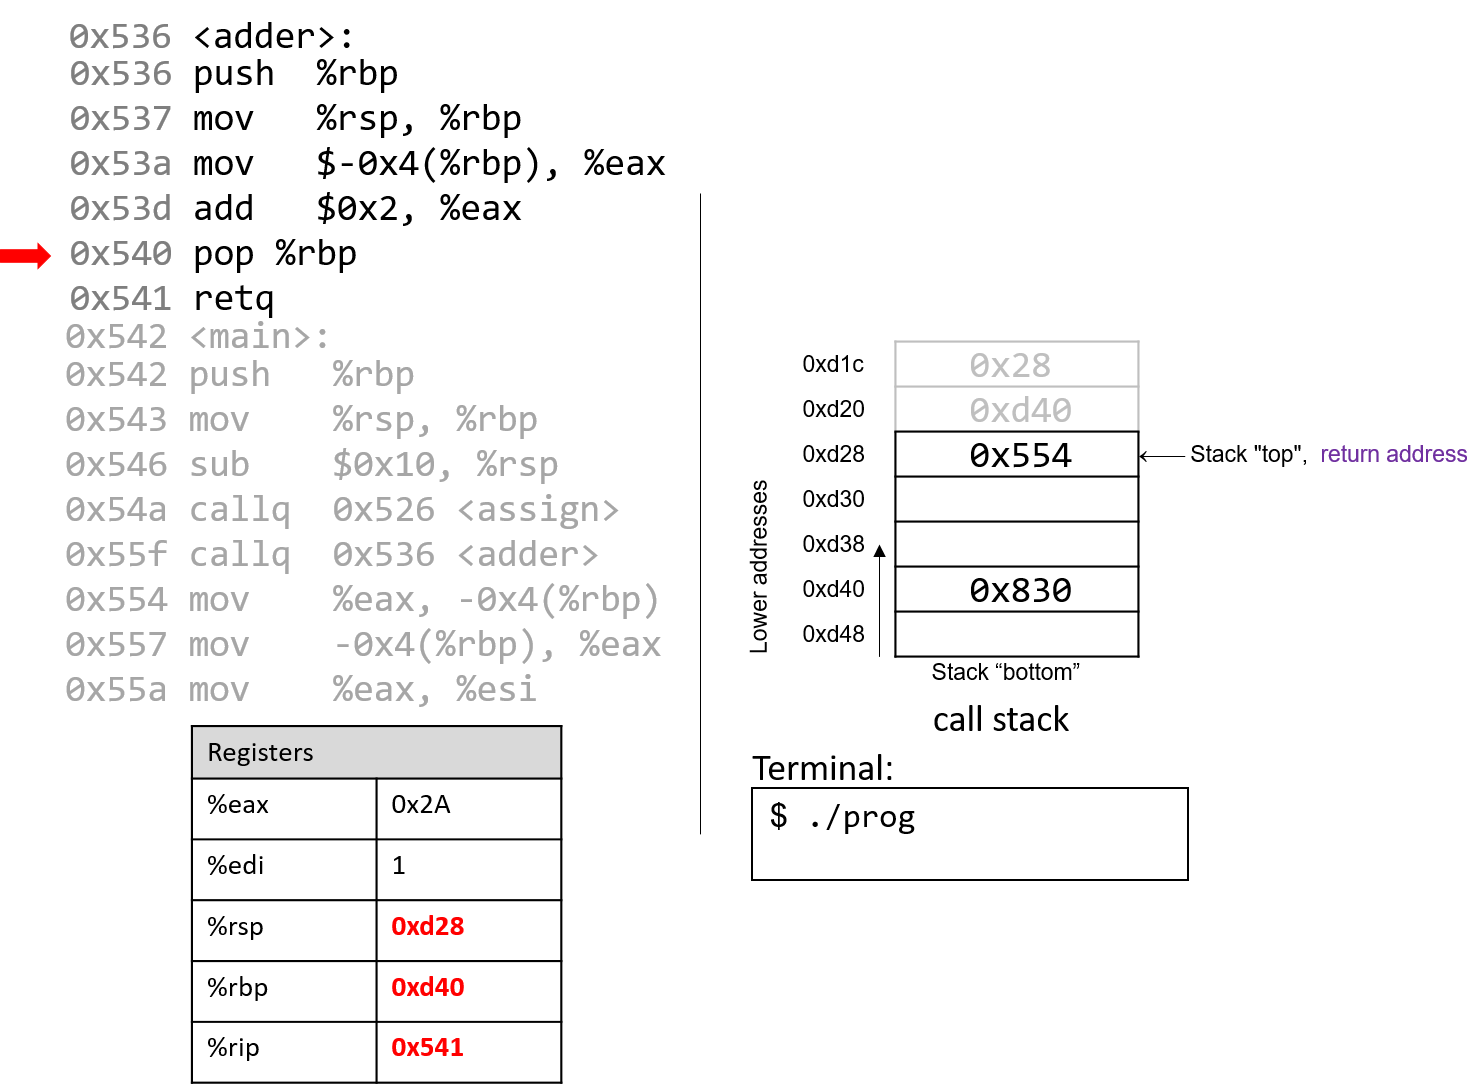
\includegraphics[scale=0.5]{img/Slide17.png}
            \end{center}

          \item We now return the value in \texttt{\%eax} and pop the base pointer of the adder stack frame, which simply updates the instruction pointer \texttt{\%rip} back to the next instruction in main. This is equivalent to \texttt{pop \%rip}, which is equivalent to moving the stack pointer \texttt{\%rsp} into \texttt{\%rip} and then shrinking the stack by 8 bytes \texttt{subq \$8, \%rsp}. 
            \begin{center}
              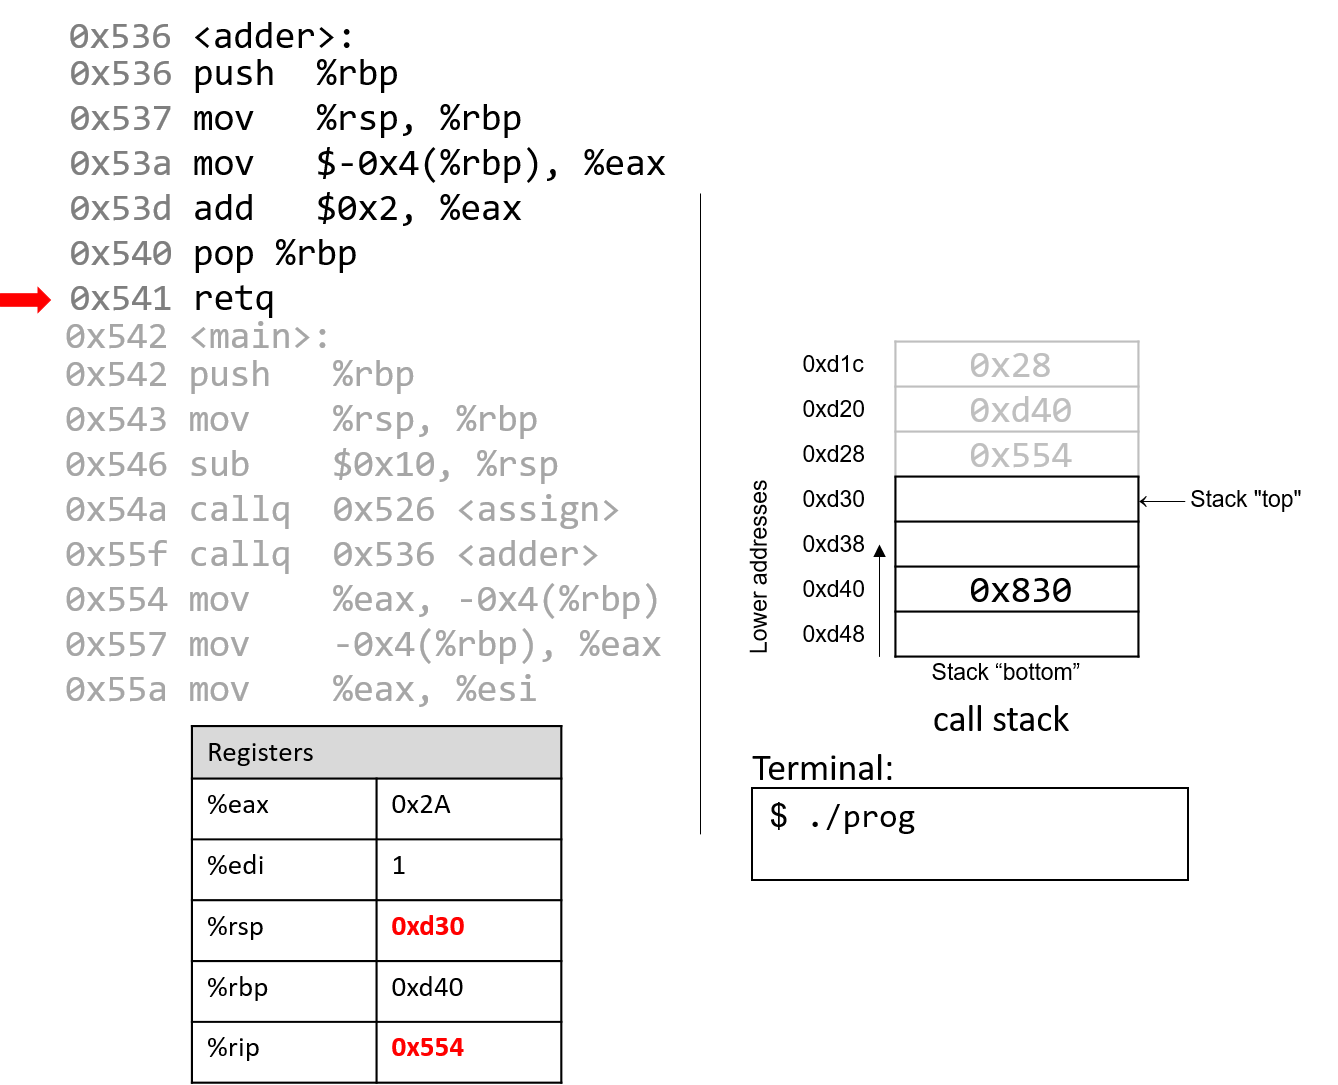
\includegraphics[scale=0.5]{img/Slide18.png}
            \end{center}

          \item Now it is relatively straightforward since we do the rest in main (except for the print statement). The current value in \texttt{\%eax} represents the return value of adder. We want to put this in the variable \texttt{x}, which we have already allocated some memory for right above the base pointer in the main stack frame. We move it there. Note that right after, it places this right back into \texttt{\%eax}.
            \begin{center}
              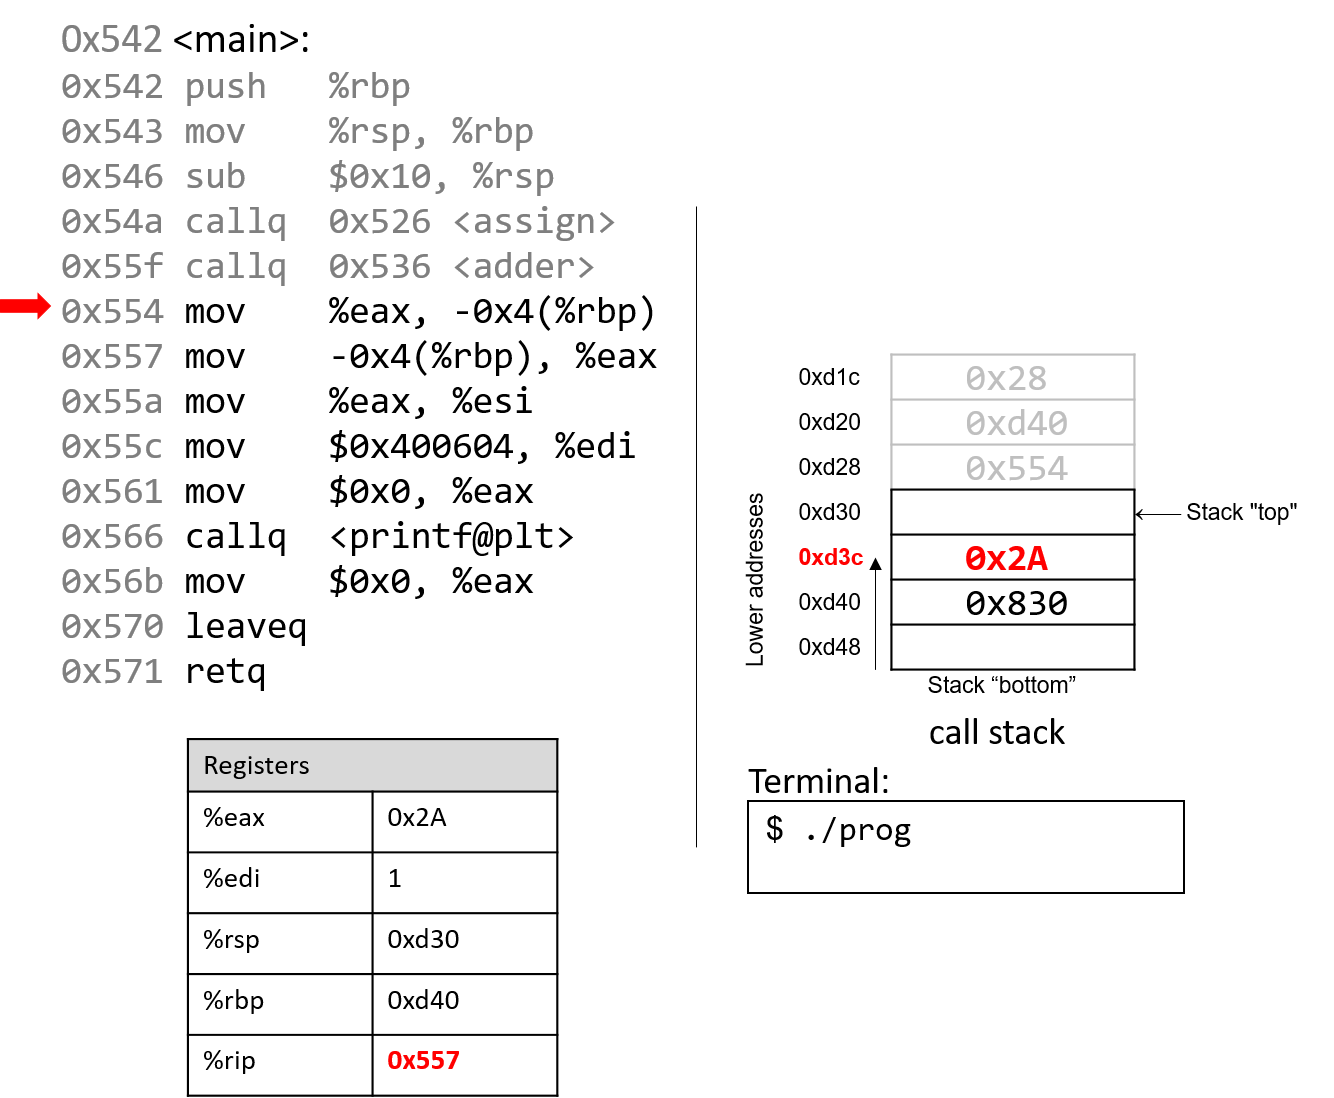
\includegraphics[scale=0.5]{img/Slide19.png}
            \end{center}

          \item the mov instruction at address 0x55a copies the value in \texttt{\%eax} (or 0x2A) to register \texttt{\%esi}, which is the 32-bit component register associated with \texttt{\%rsi} and typically stores the second parameter to a function. We can see why since this will be put into a print statement, which is a function, and \texttt{x = \%esi} is the second argument of \texttt{printf}. 
            \begin{center}
              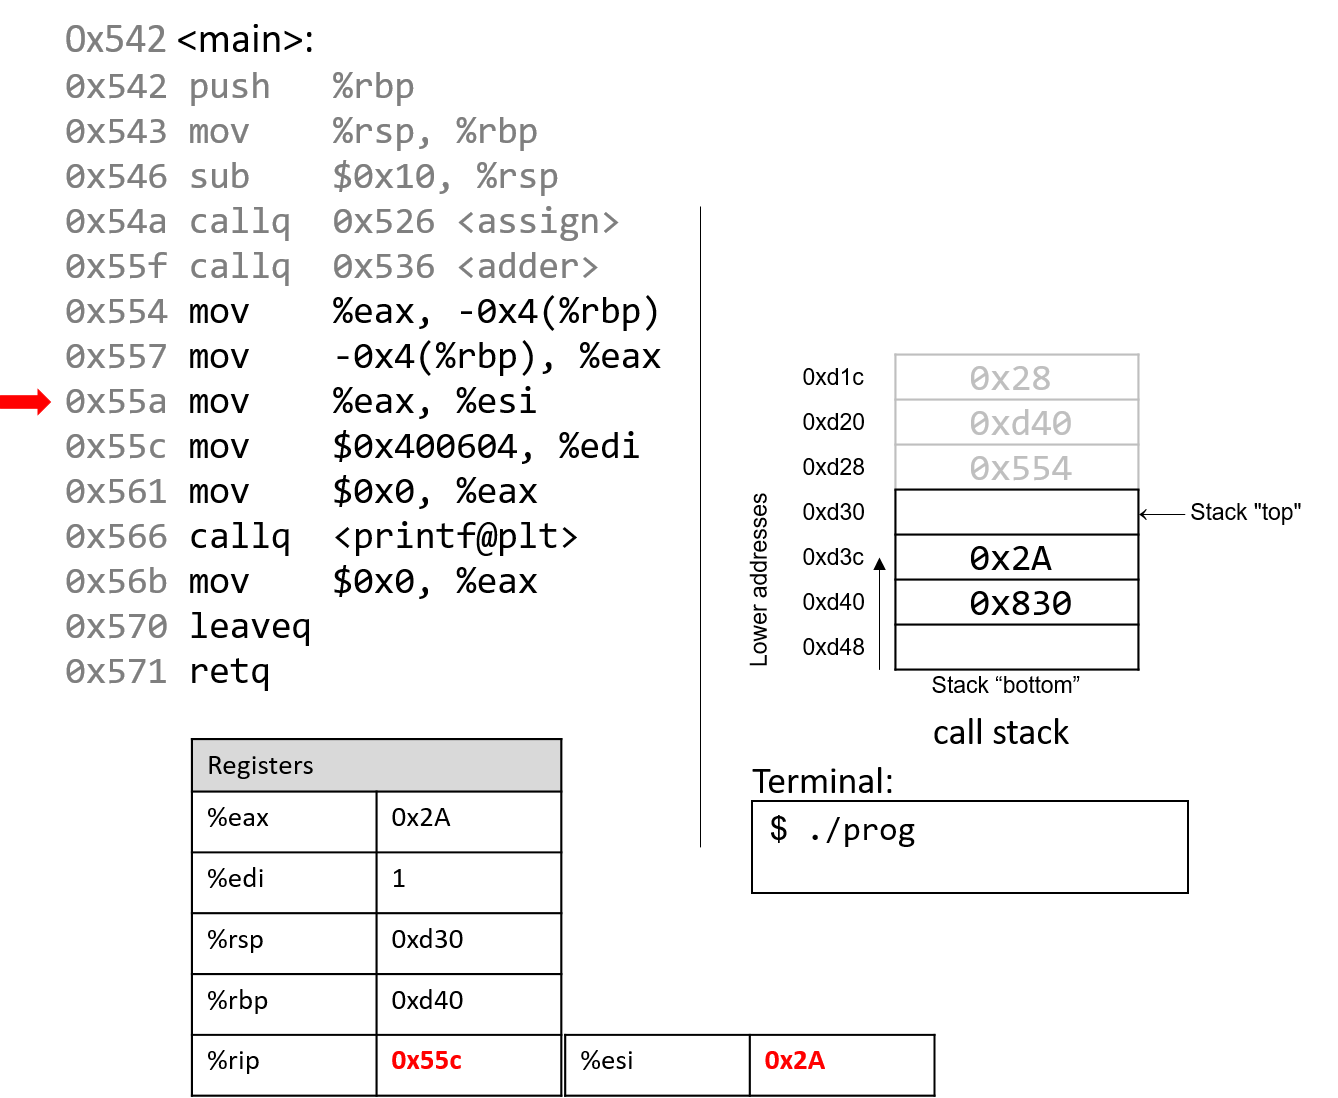
\includegraphics[scale=0.5]{img/Slide21.png}
            \end{center}

          \item Now we want to retrieve the first argument of the print function. The address at \texttt{\$0x400604} is some address in the code segment memory that holds the string \texttt{"x is \%d\textbackslash n"}. 
            \begin{center}
              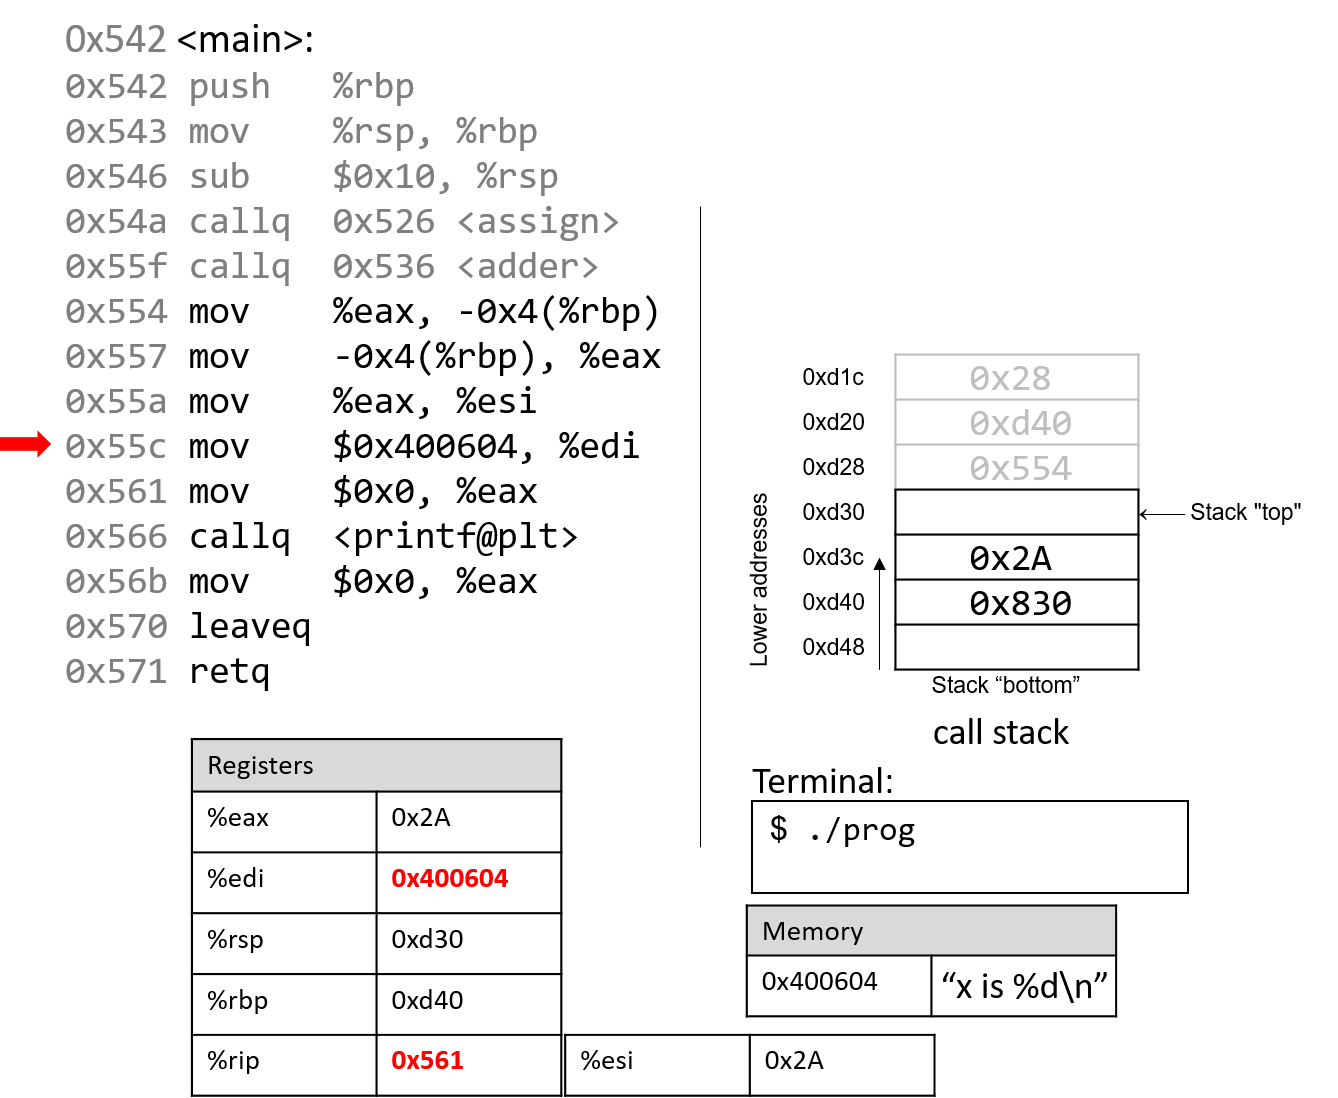
\includegraphics[scale=0.5]{img/Slide22.png}
            \end{center}

          \item Then we move $0$ into the \texttt{\%eax} register to clear it. 
            \begin{center}
              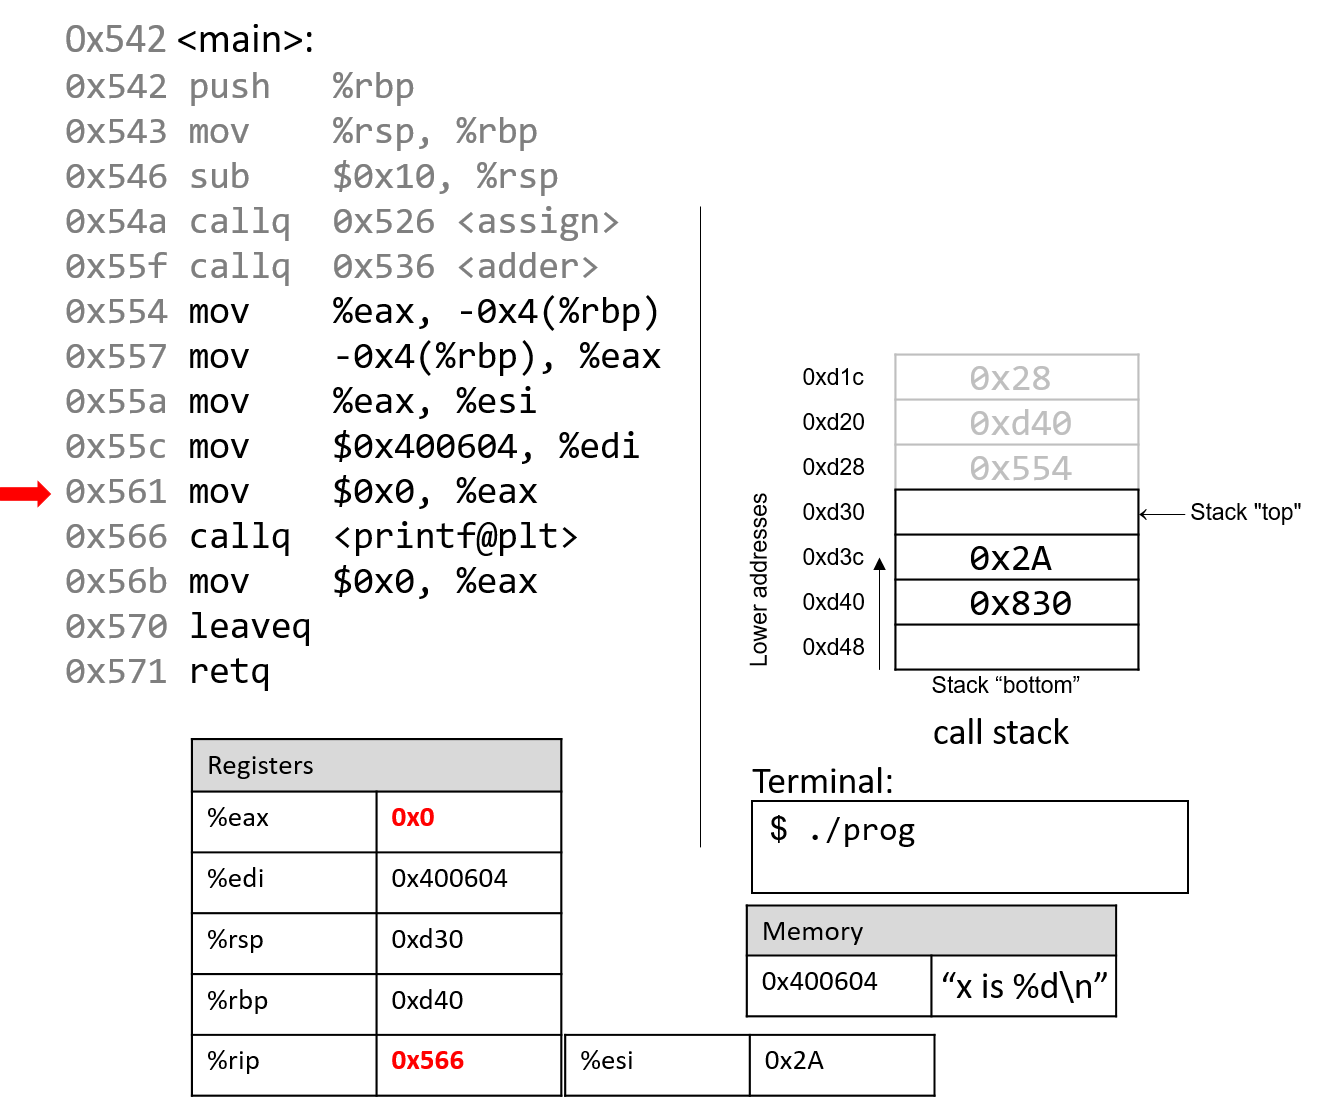
\includegraphics[scale=0.5]{img/Slide23.png}
            \end{center} 

          \item We then call the \texttt{printf} function, which we won't trace through but it outputs to stdout.  
            \begin{center}
              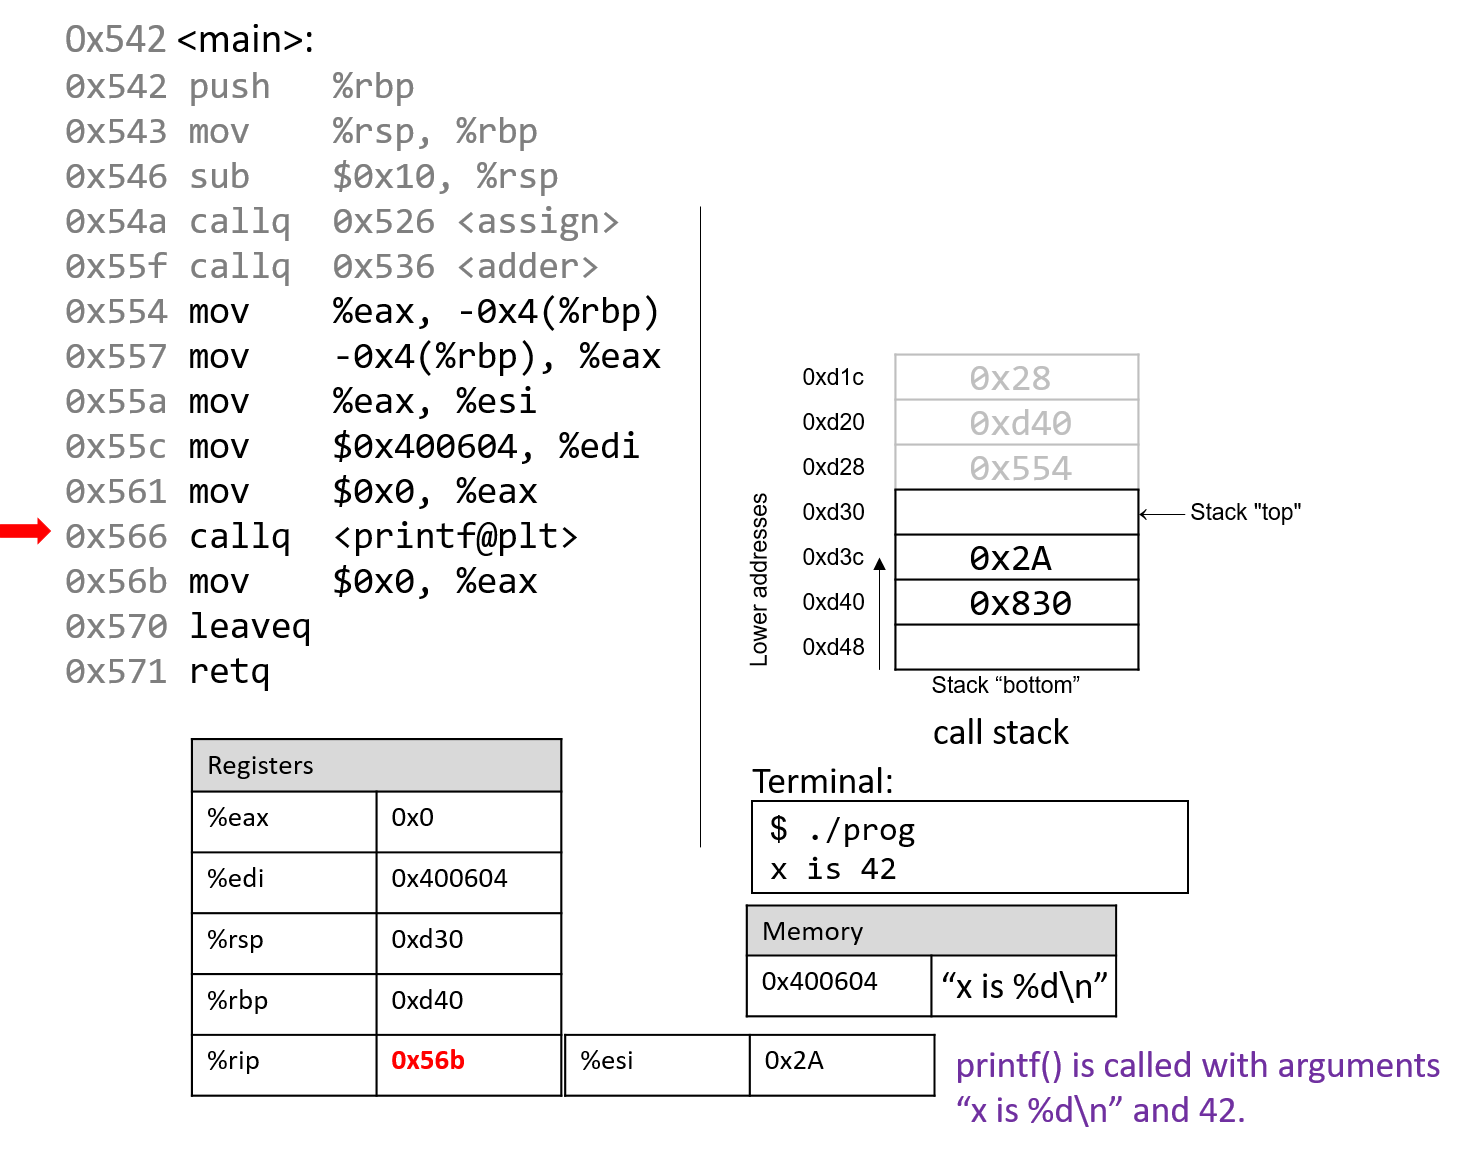
\includegraphics[scale=0.5]{img/Slide24.png}
            \end{center}

          \item The print function might have returned something, but we don't care. We want to main function to return 0, so we move 0 into \texttt{\%eax}. 
            \begin{center}
              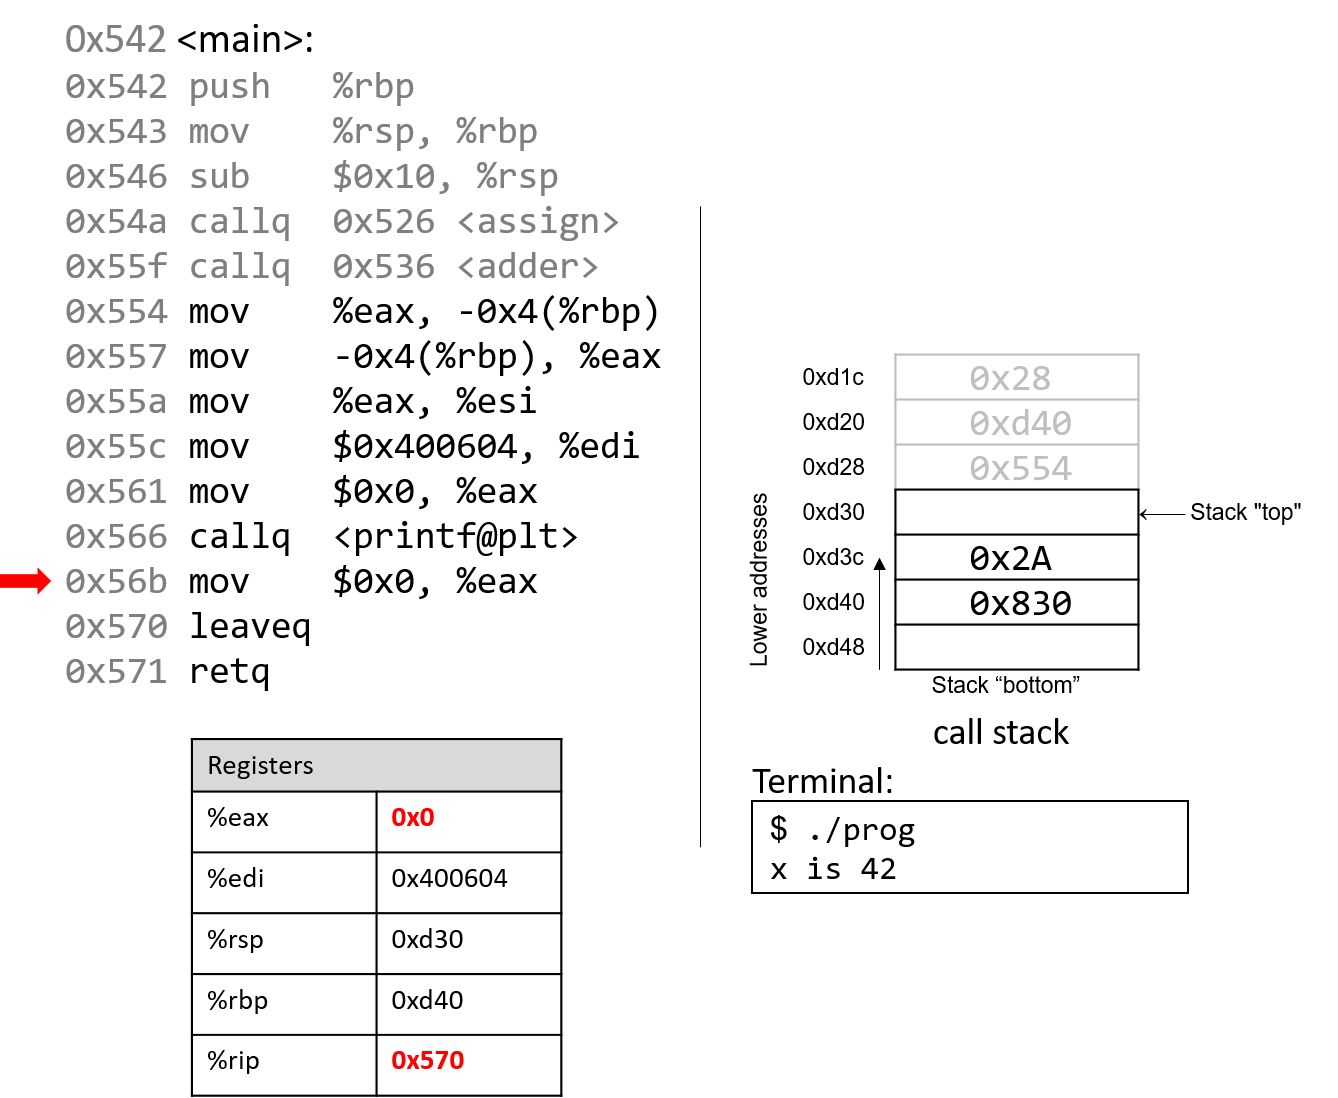
\includegraphics[scale=0.5]{img/Slide25.png}
            \end{center}

          \item Finally we execute \texttt{leaveq}, which prepares the stack for returning from the function call. It essentially moves the base pointer back to the stack pointer and then pops the base pointer off the stack. The new \texttt{\%rbp} is the original base pointer of whatever was outside the main function, \texttt{0x830}. 
            \begin{center}
              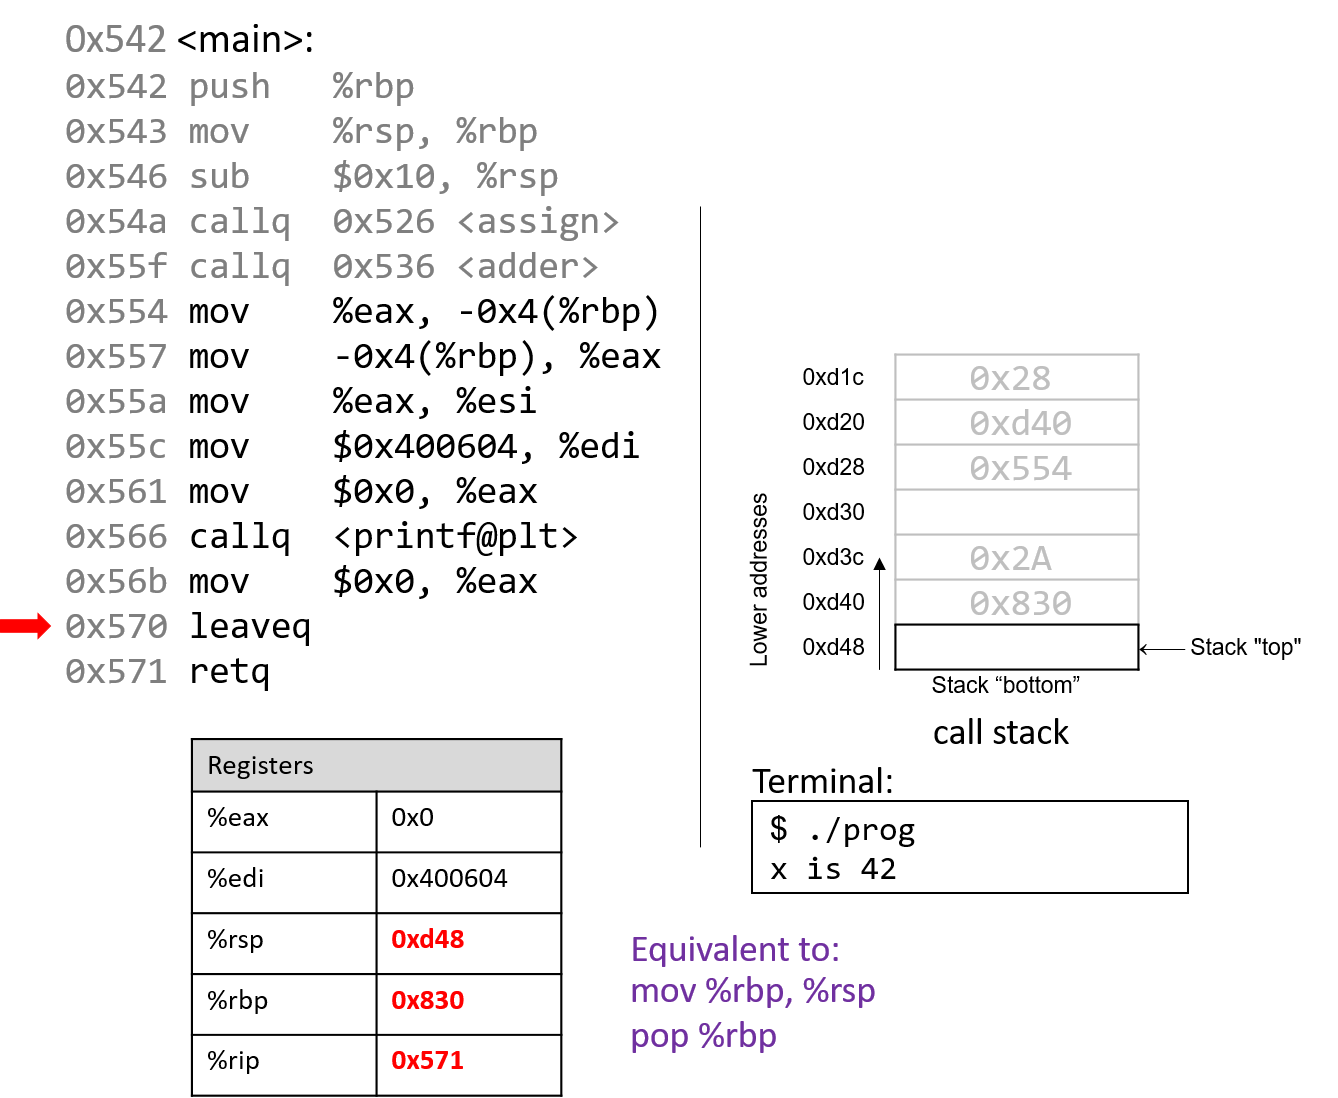
\includegraphics[scale=0.5]{img/Slide26.png}
            \end{center}

          \item Finally, we execute \texttt{retq}, which pops the return address off the stack and puts it into \texttt{\%rip}. 
        \end{enumerate}
      \end{example}

      We have omitted the details of caller and callee saved registers, but they do exist and are important for the general implementations. 

      For arrays, there's not anything new here. Let's go over some code and follow through it. 

      \begin{lstlisting}
        int sumArray(int *array, int length) {
          int i, total = 0;
          for (i = 0; i < length; i++) {
            total += array[i];
          }
          return total;
        }
      \end{lstlisting}

      This function takes the address of an array and the length of it and sums up all the elements in the array. 

      \begin{lstlisting}
        0x400686 <+0>:	push %rbp                   # save %rbp
        0x400687 <+1>:	mov  %rsp,%rbp              # update %rbp (new stack frame)
        0x40068a <+4>:	mov  %rdi,-0x18(%rbp)       # copy array to %rbp-0x18
        0x40068e <+8>:	mov  %esi,-0x1c(%rbp)       # copy length to %rbp-0x1c
        0x400691 <+11>:	movl $0x0,-0x4(%rbp)        # copy 0 to %rbp-0x4 (total)
        0x400698 <+18>:	movl $0x0,-0x8(%rbp)        # copy 0 to %rbp-0x8 (i)
        0x40069f <+25>:	jmp  0x4006be <sumArray+56> # goto <sumArray+56>
        0x4006a1 <+27>:	mov  -0x8(%rbp),%eax        # copy i to %eax
        0x4006a4 <+30>:	cltq                        # convert i to a 64-bit integer
        0x4006a6 <+32>:	lea  0x0(,%rax,4),%rdx      # copy i*4 to %rdx
        0x4006ae <+40>:	mov  -0x18(%rbp),%rax       # copy array to %rax
        0x4006b2 <+44>:	add  %rdx,%rax              # compute array+i*4, store in %rax
        0x4006b5 <+47>:	mov  (%rax),%eax            # copy array[i] to %eax
        0x4006b7 <+49>:	add  %eax,-0x4(%rbp)        # add %eax to total
        0x4006ba <+52>:	addl $0x1,-0x8(%rbp)        # add 1 to i (i+=1)
        0x4006be <+56>:	mov  -0x8(%rbp),%eax        # copy i to %eax
        0x4006c1 <+59>:	cmp  -0x1c(%rbp),%eax       # compare i to length
        0x4006c4 <+62>:	jl   0x4006a1 <sumArray+27> # if i<length goto <sumArray+27>
        0x4006c6 <+64>:	mov  -0x4(%rbp),%eax        # copy total to %eax
        0x4006c9 <+67>:	pop  %rbp                   # prepare to leave the function
        0x4006ca <+68>:	retq                        # return total
      \end{lstlisting}

    \subsubsection{ARM Instructions}

      

    \subsubsection{Buffer Overflows}

\section{Compiling and Linking}

  Now let's talk about how this compiling actually happens. \textit{Compiling} is actually an umbrella term that is misused. Turning at C file into an executable file consists of multiple intermediate steps, one of which is actually compiling, but the whole series is sometimes referred to as compiling. A more accurate term would be \textit{building}. Before we get onto it, there are two types of compilers. 

  \begin{definition}[GCC, CLang]
    The two mainstream compilers used is GCC (with the gdb debugger) and Clang (with lldb). For now, the difference is that 
    \begin{enumerate}
      \item gcc is more established. 
      \item clang is newer and has more features. 
    \end{enumerate}
    A useful flag to know is that we can always specify the name of the (final or intermediary) output file with the \texttt{-o} flag. 
  \end{definition}

  \begin{definition}[Complete Build Process]
    To actually turn a C file into an executable file, we need to go through a series of steps. We start off with the C code, which are the \texttt{.c}, \texttt{.cpp}, or \texttt{.h} files. 
    \begin{enumerate}
      \item \textbf{Preprocessing}: The precompiler step expands the \textit{preprocessor directives} (all the \texttt{\#include} and \texttt{\#define} statements) and removes comments. This results in a \texttt{.i} file. The preprocessor will replace these macros with the actual code. This results in a \texttt{.i} file.
        \begin{lstlisting}
          clang/gcc -E main.c -o main.i
        \end{lstlisting}

      \item \textbf{Compiling}: We take these and generate assembly code. This results in a \texttt{.asm} or \texttt{.s} file.
        \begin{lstlisting}
          clang/gcc -S main.c -o main.s
        \end{lstlisting}

      \item \textbf{Assembler}: We take the assembly code and generate machine code in the form of relocatable binary object code (this is machine code, not assembly). This results in a \texttt{.o} or \texttt{.obj} file.
        \begin{lstlisting}
          clang/gcc -c main.c -o main.o
        \end{lstlisting}

      \item \textbf{Linking}: We take these object files and link them together to form an executable file. This results in a \texttt{.exe} or \texttt{.out} file.
    \end{enumerate}
    The GCC or CLang compiler automates this process for us. For example, \texttt{gcc -c hello.c} generates an object file, taking care of the preprocessing, compiling, and assembling code. Then, \texttt{gcc hello.o} links the object file to generate an executable file. 
  \end{definition}

  There are a lot of questions to be asked here, and we will go through them step by step. 

  \subsection{Precompiling Stage} 

    Just like how Python package managers like conda have specific directories that they find package in, the C library also has a certain directory. 

    \begin{definition}[Standard Library Directory]
      In Linux systems, there are two main directories you look at: 
      \begin{enumerate}
        \item \texttt{/usr/include} contains the standard C library headers.
        \item \texttt{/usr/local/include} contains the headers for libraries that you install yourself.
      \end{enumerate}
      In Mac Silicon, these directories are a little bit more involved. You must first install the xcode command line developer tools, which will then create these directories. 
      \begin{enumerate}
        \item The standard C library headers are in 
          \begin{equation*}
            \texttt{/Library/Developer/CommandLineTools/SDKs/MacOSX*.sdk/usr/include}.
          \end{equation*}
      \end{enumerate}
    \end{definition}

    In here, we can find all the relevant import files like \texttt{stdio.h} and such. When we precompile, the output \texttt{.i} file represents a precompiled C file. It still has C code, but it has been optimized to 
    \begin{enumerate}
      \item Remove comments. 
      \item Replace all the \texttt{\#include} statements with the actual code. 
      \item Replace all the global variables declared in \texttt{\#define} with the actual value.
    \end{enumerate}
    Between x86 and ARM, there are no significant differences in how C files are precompiled. 

    \begin{example}
      Take a look at the following minimal example. 
      \begin{figure}[H]
        \centering 
        \noindent\begin{minipage}{.5\textwidth}
        \begin{lstlisting}[]{Code}
          #include "second.h"
          #define a 3

          int add(int x, int y) {
            return x + y;
          }

          int main() {
            // test comment
            int b = 5; 
            int c = add(a, b);
            int d = subtract(a, b); 
            return 0; 
          }
        \end{lstlisting}
        \end{minipage}
        \hfill
        \begin{minipage}{.49\textwidth}
        \begin{lstlisting}[]{Output}
          int subtract(int a, int b) {
            return a - b; 
          }
          .
          .
          .
          .
          .
          .
          .
          .
          .
          .
          .
        \end{lstlisting}
        \end{minipage}
        \caption{I have included a \texttt{main.c} file that imports statements from a \texttt{second.h} file.} 
        \label{fig:precompile_example}
      \end{figure}
      Now, I run \texttt{gcc -E main.c -o main.i} to generate the precompiled file, which gives me the following. 
      \begin{figure}[H]
        \centering 
        \begin{lstlisting}
          # 1 "main.c"
          # 1 "<built-in>" 1
          # 1 "<built-in>" 3
          # 418 "<built-in>" 3
          # 1 "<command line>" 1
          # 1 "<built-in>" 2
          # 1 "main.c" 2
          # 1 "./second.h" 1
          int subtract(int a, int b) {
            return a - b;
          }
          # 2 "main.c" 2


          int add(int x, int y) {
            return x + y;
          }

          int main() {

            int b = 5;
            int c = add(3, b);
            int d = subtract(3, b);
            return 0;
          }
        \end{lstlisting}
        \caption{The precompiled file. } 
        \label{fig:precompiled_file}
      \end{figure}
      Notice a few things: 
      \begin{enumerate}
        \item The header file \texttt{second.h} has been replaced with the actual code.
        \item The comments have indeed been removed. 
        \item The global variable \texttt{a} has been replaced with the actual value 3. 
      \end{enumerate}
    \end{example}

    This leaves us with the question of what all the rest of the lines that start with a \texttt{\#} are for. They are called \textit{preprocessor directives}.

    \begin{definition}[Preprocessor Directives]
      \textbf{Preprocessor directives} are commands that are executed before the actual compilation begins. These directives allow additional actions to be taken on the C source code before it is compiled into object code. Directives are not part of the C language itself, and they are always prefixed with a \texttt{\#} symbol. 
      \begin{enumerate}
        \item \texttt{\#include} is used to include the contents of a file into the source file. It selects portions of the file to include based on the file name.
        \item \texttt{\#define} is used to define a macro, which is a way to give a name to a constant value or a piece of code. 
        \item \texttt{\#ifdef}, \texttt{\#ifndef}, \texttt{\#else}, and \texttt{\#endif} are used for conditional compilation. 
        \item \texttt{\#error} is used to generate a compilation error. 
        \item \texttt{\#pragma} is used to give the compiler specific instructions. 
      \end{enumerate}
    \end{definition}

  \subsection{Compiling Stage} 

    Once we have precompiled, we can compile the code into assembly code. For the following two examples, we will parse through the general syntax of assembly code. It is quite different between x86 and ARM, so we will use the minimal C code 
    \begin{lstlisting}
      int add(int x, int y) {
        return x + y;
      }

      int main() {
        int a = 3;
        int b = 5; 
        int c = add(a, b);
        return 0; 
      }
    \end{lstlisting}
    for both examples. 

    \begin{example}[x86 Compiled Assembly Language]
      The assmebly code is shown. 
      \begin{lstlisting}[language={[x86masm]Assembler}]
        .
          .file	"main.c"
          .text
          .globl	add
          .type	add, @function
        add:
        .LFB0:
          .cfi_startproc
          endbr64
          pushq	%rbp
          .cfi_def_cfa_offset 16
          .cfi_offset 6, -16
          movq	%rsp, %rbp
          .cfi_def_cfa_register 6
          movl	%edi, -4(%rbp)
          movl	%esi, -8(%rbp)
          movl	-4(%rbp), %edx
          movl	-8(%rbp), %eax
          addl	%edx, %eax
          popq	%rbp
          .cfi_def_cfa 7, 8
          ret
          .cfi_endproc
        .LFE0:
          .size	add, .-add
          .globl	main
          .type	main, @function
        main:
        .LFB1:
          .cfi_startproc
          endbr64
          pushq	%rbp
          .cfi_def_cfa_offset 16
          .cfi_offset 6, -16
          movq	%rsp, %rbp
          .cfi_def_cfa_register 6
          subq	$16, %rsp
          movl	$3, -12(%rbp)
          movl	$5, -8(%rbp)
          movl	-8(%rbp), %edx
          movl	-12(%rbp), %eax
          movl	%edx, %esi
          movl	%eax, %edi
          call	add
          movl	%eax, -4(%rbp)
          movl	$0, %eax
          leave
          .cfi_def_cfa 7, 8
          ret
          .cfi_endproc
        .LFE1:
          .size	main, .-main
          .ident	"GCC: (Ubuntu 9.4.0-1ubuntu1~20.04.2) 9.4.0"
          .section	.note.GNU-stack,"",@progbits
          .section	.note.gnu.property,"a"
          .align 8
          .long	 1f - 0f
          .long	 4f - 1f
          .long	 5
        0:
          .string	 "GNU"
        1:
          .align 8
          .long	 0xc0000002
          .long	 3f - 2f
        2:
          .long	 0x3
        3:
          .align 8
        4:
      \end{lstlisting}
    \end{example}

    \begin{example}[ARM Compiled Assembly Language]
      The assembly code is shown. 
      \begin{lstlisting}[language={[x86masm]Assembler}]
        .
          .section	__TEXT,__text,regular,pure_instructions
          .build_version macos, 14, 0	sdk_version 14, 4
          .globl	_add                            ; -- Begin function add
          .p2align	2
        _add:                                   ; @add
          .cfi_startproc
        ; %bb.0:
          sub	sp, sp, #16
          .cfi_def_cfa_offset 16
          str	w0, [sp, #12]
          str	w1, [sp, #8]
          ldr	w8, [sp, #12]
          ldr	w9, [sp, #8]
          add	w0, w8, w9
          add	sp, sp, #16
          ret
          .cfi_endproc
                                                ; -- End function
          .globl	_main                           ; -- Begin function main
          .p2align	2
        _main:                                  ; @main
          .cfi_startproc
        ; %bb.0:
          sub	sp, sp, #48
          .cfi_def_cfa_offset 48
          stp	x29, x30, [sp, #32]             ; 16-byte Folded Spill
          add	x29, sp, #32
          .cfi_def_cfa w29, 16
          .cfi_offset w30, -8
          .cfi_offset w29, -16
          mov	w8, #0
          str	w8, [sp, #12]                   ; 4-byte Folded Spill
          stur	wzr, [x29, #-4]
          mov	w8, #3
          stur	w8, [x29, #-8]
          mov	w8, #5
          stur	w8, [x29, #-12]
          ldur	w0, [x29, #-8]
          ldur	w1, [x29, #-12]
          bl	_add
          mov	x8, x0
          ldr	w0, [sp, #12]                   ; 4-byte Folded Reload
          str	w8, [sp, #16]
          ldp	x29, x30, [sp, #32]             ; 16-byte Folded Reload
          add	sp, sp, #48
          ret
          .cfi_endproc
                                                ; -- End function
        .subsections_via_symbols
      \end{lstlisting}
    \end{example}
      
    We can see that in both examples, there are generally two types of codes. 
    \begin{enumerate}
      \item The regular CPU operations with registers and memory. 
      \item Some code starts off with some code that starts with a \texttt{.}. Every line that starts with a \texttt{.} are called \textit{assembler directives}. 
    \end{enumerate}
    Let's elaborate more on what these directives are. 

    \begin{definition}[Assembler Directives]
      An \textbf{assembler directives} are instructions in assembly language programming that that give commands to the assembler (which then converts this to an object file) about various aspects of the assembly process, but they do not represent actual CPU instructions that execute in the program. Unlike typical assembly language instructions that directly manipulate registers and execute arithmetic or logical operations, directives are used to organize, control, and provide necessary information for the assembly and linking of binary programs. They can manage memory allocation, define symbols, control compilation settings, and much more. 

      There are general types of directives that are common in both x86 and ARM that we should be aware about: 
      \begin{enumerate}
        \item Section directives. 
        \item Data allocation directives. 
        \item Symbol definition directives. 
        \item Macro and Include directives. 
        \item Debugging and error handling directives. 
      \end{enumerate}
    \end{definition}

    \begin{example}[x86 Assembly Directives]
      Let us elaborate on the specific directives in the x86 assembly code, some of which are in the example above. 
      \begin{enumerate}
        \item \texttt{.file "main.c"} is a directive that tells the assembler that the following code is from the file \texttt{main.c}. It is a form of metadata. 
        \item \texttt{.text} is a directive that tells the assembler that the following code is the text section (the text/code portion of memory) of the program. This is where the actual code is stored. 
        \item \texttt{.globl add} is a directive that tells the assembler that the following code is a global function called \texttt{add}.
        \item \texttt{.type add, @function} is a directive that tells the assembler that the following code is a function.
      \end{enumerate}
    \end{example}

    \begin{example}[ARM Assembly Directives]
      
    \end{example}

    You also see that there are symbols that represent memory addresses. Let's elaborate on what symbols mean. 

    \begin{definition}[Symbol]
      A \textbf{symbol} is a name that is used to refer to a memory location. It can be a function name, a global variable, or a local variable. 
      \begin{enumerate}
        \item Global symbols are symbols that can be referenced by other object files, e.g. non-static functions and global variables. 
        \item Local symbols are symbols that are only visible within the object file, e.g. static functions and local variables. The linker won't know about these types. 
        \item External symbols are referenced by this object file but defined in another object file. 
      \end{enumerate}
    \end{definition}

  \subsection{Objdump} 

    Since we will be using the \texttt{objdump} package quite a lot, it is worth mentioning the different commands you will use and store them here as a reference. For first readers, don't expect to know what each of them do, but rather look back at this for a reference. 

    \subsubsection{ELF and Mach-O Formats}

      Objdump is a command line utility that is used to display information about object files, which are often outputted in a specific format. The two main output file types are called ELF (Executable and Linkable Format) and Mach-O (Mach Object). 

      \begin{definition}[ELF]
        The \textbf{Executable and Linkable Format} (ELF) is a common standard file format for executables, object code, shared libraries, and core dumps. It is analogous to a book, with the following parts: 
        \begin{enumerate}
          \item \textbf{Header}, which is like the cover of the book. It contains metadata about the file, such as the architecture, the entry point, and the sections. 
          \item \textbf{Sections}, which are like chapters. Each section contains the content for some given purpose or use wthin the program. e.g. \texttt{.binary} is just a block of bytes, \texttt{.text} contains the machine code, \texttt{.data} contains initialized data, and \texttt{.bss} contains uninitialized data.
          \item \textbf{Symbol Table}, is like a detailed table of contents of all defined symbols such as functions, external (global) variables, local maps, etc. 
          \item \textbf{Relocation records}, which is like the index of the book that lists references to symbols. 
        \end{enumerate}
        The format is generally as such when you run \texttt{objdump -d -r hello.o} (d represents disassembly and r represents relocation entries).

        \begin{lstlisting}
          ELF header         # file type 

          .text section 
            - code goes here 

          .rodata section
            - read only data 

          .data section 
            - initialized global variables 

          .bss section 
            - uninitialized global variables

          .symtab section 
            - symbol table (symbol name, type, address) 

          .rel.text section 
            - relocation entries for .text section 
            - addresses of instructions that will need to be modified in the executable. 

          .rel.data section 
            - relocation info for .data section 
            - addresses of pointer data that will need to be modified in the merged executable. 

          .debug section 
            - info for symbolic debugging (gcc -g) 
        \end{lstlisting}
      \end{definition}
      
      \begin{definition}[Mach-O]
        
      \end{definition}

    \subsubsection{Objdump Commands}

      \begin{theorem}[File Headers with Objdump]
        Given that you have an object file, the first thing you might want to do is see the file header. You do with this \texttt{objdump -f main.o}. 
        \begin{lstlisting}
          main.o:     file format elf64-x86-64
          architecture: i386:x86-64, flags 0x00000011:
          HAS_RELOC, HAS_SYMS
          start address 0x0000000000000000
        \end{lstlisting}
      \end{theorem}

      \begin{theorem}[Section with Objdump]
        To look at the section headers to get a closer overview, you use \texttt{objdump -h main.o}. 
        \begin{lstlisting}
          main.o:     file format elf64-x86-64

          Sections:
          Idx Name          Size      VMA               LMA               File off  Algn
            0 .text         0000004b  0000000000000000  0000000000000000  00000040  2**0
                            CONTENTS, ALLOC, LOAD, RELOC, READONLY, CODE
            1 .data         00000000  0000000000000000  0000000000000000  0000008b  2**0
                            CONTENTS, ALLOC, LOAD, DATA
            2 .bss          00000000  0000000000000000  0000000000000000  0000008b  2**0
                            ALLOC
            3 .comment      0000002c  0000000000000000  0000000000000000  0000008b  2**0
                            CONTENTS, READONLY
            4 .note.GNU-stack 00000000  0000000000000000  0000000000000000  000000b7  2**0
                            CONTENTS, READONLY
            5 .note.gnu.property 00000020  0000000000000000  0000000000000000  000000b8  2**3
                            CONTENTS, ALLOC, LOAD, READONLY, DATA
            6 .eh_frame     00000058  0000000000000000  0000000000000000  000000d8  2**3
                            CONTENTS, ALLOC, LOAD, RELOC, READONLY, DATA
        \end{lstlisting}
      \end{theorem}

      \begin{theorem}[Disassembly with Objdump]
        Now you might actually want to look at the disassembly of the code, which is what we often use it for. To do this, you use \texttt{objdump -D main.o} to get the entire output. 
        \begin{enumerate}
          \item The leftmost column represents the address of the instruction. 
          \item The next column represents the machine code of the instruction. 
          \item The next column represents the assembly code of the instruction. 
        \end{enumerate}
        \begin{lstlisting}
          main.o:     file format elf64-x86-64

          Disassembly of section .text:

          0000000000000000 <add>:
             0:	f3 0f 1e fa          	endbr64 
             ...
            17:	c3                   	retq   

          0000000000000018 <main>:
            18:	f3 0f 1e fa          	endbr64 
            ...
            4a:	c3                   	retq   

          Disassembly of section .comment:

          0000000000000000 <.comment>:
             0:	00 47 43             	add    %al,0x43(%rdi)
             ...
            2a:	30 00                	xor    %al,(%rax)

          Disassembly of section .note.gnu.property:

          0000000000000000 <.note.gnu.property>:
             0:	04 00                	add    $0x0,%al
            ...

          Disassembly of section .eh_frame:

          0000000000000000 <.eh_frame>:
             0:	14 00                	adc    $0x0,%al
            ...
        \end{lstlisting}
        If you just want to look at the contents of the executable sections, then you can use \texttt{objdump -d main.o}.
        \begin{lstlisting}
          main.o:     file format elf64-x86-64

          Disassembly of section .text:

          0000000000000000 <add>:
             0:	f3 0f 1e fa          	endbr64 
             4:	55                   	push   %rbp
             5:	48 89 e5             	mov    %rsp,%rbp
             8:	89 7d fc             	mov    %edi,-0x4(%rbp)
             b:	89 75 f8             	mov    %esi,-0x8(%rbp)
             e:	8b 55 fc             	mov    -0x4(%rbp),%edx
            11:	8b 45 f8             	mov    -0x8(%rbp),%eax
            14:	01 d0                	add    %edx,%eax
            16:	5d                   	pop    %rbp
            17:	c3                   	retq   

          0000000000000018 <main>:
            18:	f3 0f 1e fa          	endbr64 
            1c:	55                   	push   %rbp
            1d:	48 89 e5             	mov    %rsp,%rbp
            20:	48 83 ec 10          	sub    $0x10,%rsp
            24:	c7 45 f4 03 00 00 00 	movl   $0x3,-0xc(%rbp)
            2b:	c7 45 f8 05 00 00 00 	movl   $0x5,-0x8(%rbp)
            32:	8b 55 f8             	mov    -0x8(%rbp),%edx
            35:	8b 45 f4             	mov    -0xc(%rbp),%eax
            38:	89 d6                	mov    %edx,%esi
            3a:	89 c7                	mov    %eax,%edi
            3c:	e8 00 00 00 00       	callq  41 <main+0x29>
            41:	89 45 fc             	mov    %eax,-0x4(%rbp)
            44:	b8 00 00 00 00       	mov    $0x0,%eax
            49:	c9                   	leaveq 
            4a:	c3                   	retq 
        \end{lstlisting}

        If you want to see the source code intermixed with disassembly, then you can use the \texttt{-S} flag, but make sure that the object file is a generated with debugging information, i.e. use \texttt{gcc -c -g main.c -o main.o}. 
        \begin{figure}[H]
          \centering 
          \begin{lstlisting}
            main.o:     file format elf64-x86-64


            Disassembly of section .text:

            0000000000000000 <add>:
            int add(int x, int y) {
               0:	f3 0f 1e fa          	endbr64 
               4:	55                   	push   %rbp
               5:	48 89 e5             	mov    %rsp,%rbp
               8:	89 7d fc             	mov    %edi,-0x4(%rbp)
               b:	89 75 f8             	mov    %esi,-0x8(%rbp)
              return x + y; 
               e:	8b 55 fc             	mov    -0x4(%rbp),%edx
              11:	8b 45 f8             	mov    -0x8(%rbp),%eax
              14:	01 d0                	add    %edx,%eax
            }
              16:	5d                   	pop    %rbp
              17:	c3                   	retq   

            0000000000000018 <main>:

            int main() {
              18:	f3 0f 1e fa          	endbr64 
              1c:	55                   	push   %rbp
              1d:	48 89 e5             	mov    %rsp,%rbp
              20:	48 83 ec 10          	sub    $0x10,%rsp
              int a = 3; 
              24:	c7 45 f4 03 00 00 00 	movl   $0x3,-0xc(%rbp)
              int b = 5; 
              2b:	c7 45 f8 05 00 00 00 	movl   $0x5,-0x8(%rbp)
              int c = add(a, b); 
              32:	8b 55 f8             	mov    -0x8(%rbp),%edx
              35:	8b 45 f4             	mov    -0xc(%rbp),%eax
              38:	89 d6                	mov    %edx,%esi
              3a:	89 c7                	mov    %eax,%edi
              3c:	e8 00 00 00 00       	callq  41 <main+0x29>
              41:	89 45 fc             	mov    %eax,-0x4(%rbp)
              return 0; 
              44:	b8 00 00 00 00       	mov    $0x0,%eax
            }
              49:	c9                   	leaveq 
              4a:	c3                   	retq  
          \end{lstlisting}
          \caption{Disassembly of the object file back into assembly using \texttt{objdump -d -S main.o}.} 
          \label{fig:disassembly_example_intermixed}
        \end{figure}
        Note that you can always see this disassembly with debuggers like gdb or lldb, but objdump generally works for all architectures. 
      \end{theorem}

      \begin{theorem}[Symbol Table]
        If you want to look at all the symbols existing within the object file, you use \texttt{objdump -t main.o} (t for table of symbols). 
        \begin{enumerate}
          \item The leftmost column represents the address of the symbol. 
          \item The next column represents the type of the symbol. The \texttt{g} and \texttt{l} represent global and local symbols, respectively. The \texttt{O} and \texttt{F} represent object and function symbols, while the \texttt{UND} and \texttt{ABS} represent undefined and absolute symbols. 
          \item The next column represents the section that the symbol is in. 
          \item The next column represents the size of the symbol. 
          \item The last column represents the name of the symbol. 
        \end{enumerate}
        \begin{lstlisting}
          main.o:     file format elf64-x86-64

          SYMBOL TABLE:
          0000000000000000 l    df *ABS*	0000000000000000 main.c
          0000000000000000 l    d  .text	0000000000000000 .text
          0000000000000000 l    d  .data	0000000000000000 .data
          0000000000000000 l    d  .bss	0000000000000000 .bss
          0000000000000000 l    d  .note.GNU-stack	0000000000000000 .note.GNU-stack
          0000000000000000 l    d  .note.gnu.property	0000000000000000 .note.gnu.property
          0000000000000000 l    d  .eh_frame	0000000000000000 .eh_frame
          0000000000000000 l    d  .comment	0000000000000000 .comment
          0000000000000000 g     F .text	0000000000000018 add
          0000000000000018 g     F .text	0000000000000033 main
        \end{lstlisting}
      \end{theorem}

      \begin{theorem}[Relocation Table]
        If you want to look then at the relocation table, then you use \texttt{objdump -r main.o}. 
        \begin{enumerate}
          \item The leftmost column represents the offset of the relocation (i.e. the location within the section where this relocation needs to be applied). 
          \item The second column represents the type of relocation. 
          \item The third column represents the symbol that this relocation references. 
        \end{enumerate}
        \begin{lstlisting}
          main.o:     file format elf64-x86-64

          RELOCATION RECORDS FOR [.text]:
          OFFSET           TYPE              VALUE 
          000000000000003d R_X86_64_PLT32    add-0x0000000000000004


          RELOCATION RECORDS FOR [.eh_frame]:
          OFFSET           TYPE              VALUE 
          0000000000000020 R_X86_64_PC32     .text
          0000000000000040 R_X86_64_PC32     .text+0x0000000000000018
        \end{lstlisting}
      \end{theorem}

  \subsection{Assembling Stage and Object Files}

    Now, once you have gotten the object file, you cannot simply open it up in a text edit as it is in machine code. To actually interpret anything from it, you must \textbf{disassmble} it, meaning that you convert the machine code back into assembly code. The main software that you use to do this is \texttt{objdump}. Let's take a look again at the object file. 

    \begin{figure}[H]
      \centering 
      \begin{lstlisting}
        Disassembly of section .text:

        0000000000000000 <add>:
           0:	f3 0f 1e fa          	endbr64 
           4:	55                   	push   %rbp
           5:	48 89 e5             	mov    %rsp,%rbp
           8:	89 7d fc             	mov    %edi,-0x4(%rbp)
           b:	89 75 f8             	mov    %esi,-0x8(%rbp)
           e:	8b 55 fc             	mov    -0x4(%rbp),%edx
          11:	8b 45 f8             	mov    -0x8(%rbp),%eax
          14:	01 d0                	add    %edx,%eax
          16:	5d                   	pop    %rbp
          17:	c3                   	retq   

        0000000000000018 <main>:
          18:	f3 0f 1e fa          	endbr64 
          1c:	55                   	push   %rbp
          1d:	48 89 e5             	mov    %rsp,%rbp
          20:	48 83 ec 10          	sub    $0x10,%rsp
          24:	c7 45 f4 03 00 00 00 	movl   $0x3,-0xc(%rbp)
          2b:	c7 45 f8 05 00 00 00 	movl   $0x5,-0x8(%rbp)
          32:	8b 55 f8             	mov    -0x8(%rbp),%edx
          35:	8b 45 f4             	mov    -0xc(%rbp),%eax
          38:	89 d6                	mov    %edx,%esi
          3a:	89 c7                	mov    %eax,%edi
          3c:	e8 00 00 00 00       	callq  41 <main+0x29>
          41:	89 45 fc             	mov    %eax,-0x4(%rbp)
          44:	b8 00 00 00 00       	mov    $0x0,%eax
          49:	c9                   	leaveq 
          4a:	c3                   	retq  
      \end{lstlisting}
      \caption{Disassembly of the object file back into assembly using \texttt{objdump -d main.o}. }
      \label{fig:disassembly_example-2}
    \end{figure}

    Let's note a couple things. 
    \begin{enumerate}
      \item The functions are organized by their starting address followed by their name, e.g.  
        \begin{lstlisting}
          0000000000000000 <add>:
        \end{lstlisting}
        Within each function, each line of assembly code is shown. To find the total memory the function takes up, you can just take the address of the last line and subtract it from the address of the first line. Or you can literally count the number of bytes in each line (remember 2 hex is 1 byte). 
      \item The line that calls the \texttt{add} function is \texttt{0x0} (\texttt{00 00 00 00}), with is the \textit{relative target address} intended to be filled in by the linker. The actual assembly line just says that the function continues on to the next line at address \texttt{0x41}. This is because the object file is not aware of where it will be loaded into memory, and all lines with this opcode \texttt{e8 00 00 00 00} is intended to be filled in by the linker. 
      \item Look at address \texttt{0x3c}. It is calling another function, but the values starting from address \texttt{0x3d} is \texttt{00 00 00 00}, which is not the actual address of the function but also a dummy address. This is because the object file is not aware of where the function is located in memory.
    \end{enumerate}

  \subsection{Linking Stage and Relocation}

    \subsubsection{Relocation}

      If the object file is already in machine code, then why do we need a separate linking stage that converts \texttt{main.o} into \texttt{main} the binary? The reason is stated in the previous section: because the object files uses relative memory addressing and does not know about which memory is accessed in other object files, we need to \textbf{relocate} the symbols in the object file to their proper addresses. So how does the linker actually know how to relocate these symbols into their proper addresses? It uses the \textit{relocation table}, which contains information about the addresses that need to be modified in the object file. 

      \begin{figure}[H]
        \centering 
        \begin{lstlisting}
          main.o:     file format elf64-x86-64

          RELOCATION RECORDS FOR [.text]:
          OFFSET           TYPE              VALUE 
          000000000000003d R_X86_64_PLT32    add-0x0000000000000004


          RELOCATION RECORDS FOR [.eh_frame]:
          OFFSET           TYPE              VALUE 
          0000000000000020 R_X86_64_PC32     .text
          0000000000000040 R_X86_64_PC32     .text+0x0000000000000018
        \end{lstlisting}
        \caption{Relocation table for \texttt{main.o} object file. } 
        \label{fig:relocation_table}
      \end{figure}

      Let's talk about how to actually read this table. We can look at the first entry, which shows an offset of \texttt{0x3d}. This represents the offset from the beginning of the \texttt{.text} section where the relocation needs to be applied. Looking back at the disassembly file, this address \texttt{0x3d} is precisely where there was a dummy address \texttt{00 00 00 00}. We want to replace this with the actual address defined in the \texttt{VALUE} column, which is \texttt{add} (with a slight offset of \texttt{0x4}, which is typically used to compensate for the PC-relative addressing mode where the CPU might be adding the length of the instruction to the program counter (PC) before the relocation value is applied). The type of relocation won't be covered in our scope. Let's go through each relocation entry: 

      \begin{enumerate}
        \item The first entry is for the \texttt{add} function. If we look at the disassembly, within the \texttt{main} function, the address \texttt{0x3d} is where the \texttt{add} function is called. The linker will replace the dummy address with the actual address of the \texttt{add} function.
        \begin{lstlisting}
          Disassembly of section .text:

          0000000000000000 <add>:
             0:	f3 0f 1e fa          	endbr64 
             4:	55                   	push   %rbp
             5:	48 89 e5             	mov    %rsp,%rbp
             8:	89 7d fc             	mov    %edi,-0x4(%rbp)
             b:	89 75 f8             	mov    %esi,-0x8(%rbp)
             e:	8b 55 fc             	mov    -0x4(%rbp),%edx
            11:	8b 45 f8             	mov    -0x8(%rbp),%eax
            14:	01 d0                	add    %edx,%eax
            16:	5d                   	pop    %rbp
            17:	c3                   	retq   

          0000000000000018 <main>:
            18:	f3 0f 1e fa          	endbr64 
            1c:	55                   	push   %rbp
            1d:	48 89 e5             	mov    %rsp,%rbp
            20:	48 83 ec 10          	sub    $0x10,%rsp
            24:	c7 45 f4 03 00 00 00 	movl   $0x3,-0xc(%rbp)
            2b:	c7 45 f8 05 00 00 00 	movl   $0x5,-0x8(%rbp)
            32:	8b 55 f8             	mov    -0x8(%rbp),%edx
            35:	8b 45 f4             	mov    -0xc(%rbp),%eax
            38:	89 d6                	mov    %edx,%esi
            3a:	89 c7                	mov    %eax,%edi
            3c:	e8 00 00 00 00       	callq  41 <main+0x29>     <-- here
            41:	89 45 fc             	mov    %eax,-0x4(%rbp)
            44:	b8 00 00 00 00       	mov    $0x0,%eax
            49:	c9                   	leaveq 
            4a:	c3                   	retq  
        \end{lstlisting}
        \item The second and third entries are for the \texttt{.eh\_frame} section. We can see that the offset of \texttt{0x20} and \texttt{0x40} represents the following lines below. They also have dummy addresses that need to be replaced. They are replaced by the address \texttt{.text}, which represents the first address in the \texttt{.text} section, i.e. the address of the \texttt{add} function, and the address \texttt{.text+0x18}, which represents the address of the \texttt{main} function.
        \begin{lstlisting}
          Disassembly of section .eh_frame:

          0000000000000000 <.eh_frame>:
             0:	14 00                	adc    $0x0,%al
             2:	00 00                	add    %al,(%rax)
             4:	00 00                	add    %al,(%rax)
             6:	00 00                	add    %al,(%rax)
             8:	01 7a 52             	add    %edi,0x52(%rdx)
             b:	00 01                	add    %al,(%rcx)
             d:	78 10                	js     1f <.eh_frame+0x1f>
             f:	01 1b                	add    %ebx,(%rbx)
            11:	0c 07                	or     $0x7,%al
            13:	08 90 01 00 00 1c    	or     %dl,0x1c000001(%rax)
            19:	00 00                	add    %al,(%rax)
            1b:	00 1c 00             	add    %bl,(%rax,%rax,1)
            1e:	00 00                	add    %al,(%rax)
            20:	00 00                	add    %al,(%rax)     <-- here for 2nd entry
            22:	00 00                	add    %al,(%rax)
            24:	18 00                	sbb    %al,(%rax)
            26:	00 00                	add    %al,(%rax)
            28:	00 45 0e             	add    %al,0xe(%rbp)
            2b:	10 86 02 43 0d 06    	adc    %al,0x60d4302(%rsi)
            31:	4f 0c 07             	rex.WRXB or $0x7,%al
            34:	08 00                	or     %al,(%rax)
            36:	00 00                	add    %al,(%rax)
            38:	1c 00                	sbb    $0x0,%al
            3a:	00 00                	add    %al,(%rax)
            3c:	3c 00                	cmp    $0x0,%al
            3e:	00 00                	add    %al,(%rax)
            40:	00 00                	add    %al,(%rax)     <-- here for 3rd entry
            42:	00 00                	add    %al,(%rax)
            44:	33 00                	xor    (%rax),%eax
        \end{lstlisting}
      \end{enumerate}
      Therefore, we can see that the object file generates a ``skeleton'' code that contains all the instructions, with some dummy addresses that need to be replaced. The relocation table $T$ tells us exactly where these dummy addresses are in the code and what they need to be replaced with. Therefore, if we want to call a function \texttt{printf} that is in the text section at address \texttt{0x30}, then we can actually look at the value at \texttt{T[30]} to see where the actual address is. At this point, note that we still do not know the actual memory address of \texttt{add}. This is determined by the linker. 

    \subsubsection{Linking with One Object File}

      Now let's see what happens once we link the object file \texttt{main.o} into the final executable \texttt{main}. If we disassemble it, then we can see a few things: 
      \begin{enumerate}
        \item The addresses of all the functions have been changed. \texttt{add} starts on address \texttt{0x1129} rather than \texttt{0x0} and \texttt{main} starts on address \texttt{0x1141} rather than \texttt{0x18}. 
        \item The dummy address \texttt{0x0} of the call to function \texttt{add} in \texttt{main} have been replaced with the actual addresses \texttt{0x1129}. 
      \end{enumerate}

      \begin{lstlisting}
        0000000000001129 <add>:
          1129:	f3 0f 1e fa          	endbr64 
          112d:	55                   	push   %rbp
          112e:	48 89 e5             	mov    %rsp,%rbp
          1131:	89 7d fc             	mov    %edi,-0x4(%rbp)
          1134:	89 75 f8             	mov    %esi,-0x8(%rbp)
          1137:	8b 55 fc             	mov    -0x4(%rbp),%edx
          113a:	8b 45 f8             	mov    -0x8(%rbp),%eax
          113d:	01 d0                	add    %edx,%eax
          113f:	5d                   	pop    %rbp
          1140:	c3                   	retq   

        0000000000001141 <main>:
          1141:	f3 0f 1e fa          	endbr64 
          1145:	55                   	push   %rbp
          1146:	48 89 e5             	mov    %rsp,%rbp
          1149:	48 83 ec 10          	sub    $0x10,%rsp
          114d:	c7 45 f4 03 00 00 00 	movl   $0x3,-0xc(%rbp)
          1154:	c7 45 f8 05 00 00 00 	movl   $0x5,-0x8(%rbp)
          115b:	8b 55 f8             	mov    -0x8(%rbp),%edx
          115e:	8b 45 f4             	mov    -0xc(%rbp),%eax
          1161:	89 d6                	mov    %edx,%esi
          1163:	89 c7                	mov    %eax,%edi
          1165:	e8 bf ff ff ff       	callq  1129 <add>     <-- replaced with actual address
          116a:	89 45 fc             	mov    %eax,-0x4(%rbp)
          116d:	b8 00 00 00 00       	mov    $0x0,%eax
          1172:	c9                   	leaveq 
          1173:	c3                   	retq   
          1174:	66 2e 0f 1f 84 00 00 	nopw   %cs:0x0(%rax,%rax,1)
          117b:	00 00 00 
          117e:	66 90                	xchg   %ax,%ax 
      \end{lstlisting}

    \subsubsection{Global vs External Symbols}

      So far, we have talked about using the \texttt{\#include} as a precompiling command that says ``put all the text from this other file right here.'' Take the following code for instance. 

      \begin{figure}[H]
        \centering 
        \noindent\begin{minipage}{.5\textwidth}
        \begin{lstlisting}[]{Code}
          // file1.c 
          #include "sum.h" 

          int array[2] = {1, 2}; 

          int main() {
            int val = sum(array, 2); 
            return val; 
          }
        \end{lstlisting}
        \end{minipage}
        \hfill
        \begin{minipage}{.49\textwidth}
        \begin{lstlisting}[]{Output}
          // sum.h 
          int sum(int *a, int n) {
            int i, s = 0; 
            for (i = 0; i < n; i++) {
              s += a[i]; 
            }
            return s; 
          }
          .
        \end{lstlisting}
        \end{minipage}
        \caption{Including a header file in \texttt{file1.c} to import functions and variables.}
        \label{fig:include_example}
      \end{figure}

      However, there is another way to do this. We can use \textit{external symbols} to access. Rather than simply copying and pasting the code into the file, the \texttt{extern} keyword marks that the variable or function exists externally to this source file and does not allocate storage for it. 

      \begin{figure}[H]
        \centering 
        \noindent\begin{minipage}{.50\textwidth}
        \begin{lstlisting}[]{Code}
          // main.c
          extern int sum(int *array, int n); 

          int array[2] = {1, 2};

          int main(void) {
            int val = sum(array, 2); 
            return val; 
          }
        \end{lstlisting}
        \end{minipage}
        \hfill
        \begin{minipage}{.49\textwidth}
        \begin{lstlisting}[]{Output}
          // sum.c
          int sum(int *array, int n) {
            int i, s = 0 ; 
            for (int i = 0; i < n; i++) {
                s += array[i];
              }
            return s;
          }
          .
        \end{lstlisting}
        \end{minipage}
        \caption{Using external symbols to access functions and variables.} 
        \label{fig:external_symbols_example}
      \end{figure}
      
      One is not a replacement for the other, so what advantage does this have? Well, as we will see, if we have multiple object (source) files, say \texttt{A.c}, \texttt{B.c}, and \texttt{C.c}, that need to reference the same function or variable \texttt{var} in \texttt{ext.c}, then how would we do this? If we simply put \texttt{\#include "ext.h"} in all the files, then we would have multiple copies of the same code. This means that for each source there would be its own copy of \texttt{var} created and the linker would be unable to resolve this symbol. However, if we put \texttt{extern int var; } at the top of each source file, then only one copy of \texttt{var} would be created (in \texttt{ext.c}), which creates a single instance of \texttt{var} for the linker to resolve. \footnote{https://stackoverflow.com/questions/1330114/whats-the-difference-between-using-extern-and-including-header-files}

      Therefore, there are three types of symbols (variables, functions, etc.) that we need to consider: 
      \begin{enumerate}
        \item \textbf{Global symbols} that are defined in the global scope of a C file. 
        \item \textbf{Local symbols} that are defined in the local scope of a C file, e.g. within functions, loops, etc. 
        \item \textbf{External symbols} that are defined in another C file referenced by the \texttt{extern} keyword.
      \end{enumerate}
      Linkers will only know about global and external symbols, and will have no idea that any local symbols exist. With the information of these two types of symbols and the relocation tables of each object file, the linker can then resolve the addresses of all the symbols in the final binary. 

      The two types of symbols that the linker will know about are the global and external symbols. We can see that external symbols can be problematic if the object files don't know about each other. 

      \begin{example}[Global and Local Symbols]
        Consider the following code where the left file includes the right file. 

        \noindent\begin{minipage}{.5\textwidth}
        \begin{lstlisting}[]{Code}
          // main.c 
          #include "sum.h" 

          int array[2] = {1, 2}; 

          int main() {
            int val = sum(array, 2); 
            return val; 
          }
        \end{lstlisting}
        \end{minipage}
        \hfill
        \begin{minipage}{.49\textwidth}
        \begin{lstlisting}[]{Output}
          // sum.h 
          int sum(int *a, int n) {
            int i, s = 0; 
            for (i = 0; i < n; i++) {
              s += a[i]; 
            }
            return s; 
          }
          .
        \end{lstlisting}
        \end{minipage}
        In the left file, 
        \begin{enumerate}
          \item We define the global symbol \texttt{main()}. 
          \item Inside main, \texttt{val} is a local symbol so the linker knows nothing about it. 
          \item The \texttt{sum} function is an external symbol, and it references a global symbol that's defined in \texttt{sum} the right file. 
          \item The \texttt{array} is a global symbol that is defined in the right file. 
        \end{enumerate}
        In the right file, the linker knows nothing of the local symbols \texttt{i} or \texttt{s}. 
      \end{example}

    \subsubsection{Linking with Multiple Object Files}

      We have seen the case of linking when we simply have one object file. The relocation was simple since the \texttt{.text} section is contiguous and so we needed simple translations of addresses to relocate \texttt{add} and \texttt{main}, along with whatever other sections and files. Now let's consider the case where we have multiple object files.

      \noindent\begin{minipage}{.50\textwidth}
      \begin{lstlisting}[]{Code}
        // main.c
        extern int sum(int *array, int n); 

        int array[2] = {1, 2};

        int main(void) {
          int val = sum(array, 2); 
          return val; 
        }
      \end{lstlisting}
      \end{minipage}
      \hfill
      \begin{minipage}{.49\textwidth}
      \begin{lstlisting}[]{Output}
        // sum.c
        int sum(int *array, int n) {
          int i, s = 0 ; 
          for (int i = 0; i < n; i++) {
              s += array[i];
            }
          return s;
        }
        .
      \end{lstlisting}
      \end{minipage}

      Now they have their own object files shown below, where I also put the source code lines to make it easier to parse. Note that again, in \texttt{main.o} the call to function \texttt{sum} is a dummy address that needs to be replaced. Furthermore, in both \texttt{main.o} and \texttt{sum.o}, the \texttt{.text} section is at address \texttt{0x0}, where the addresses of the function \texttt{main} and \texttt{sum} are, respectively. This causes an overload in the address space. 

      To demonstrate what happens, we look at how the disassembly, symbol tables, and relocation tables are updated before (with the object files) and after (in the binary) linking.  

      \begin{example}[Disassembly of Object Files]
        In here, note that both the \texttt{array} and \texttt{sum} are not initialized and are therefore set to dummy addresses. 
        \begin{lstlisting}
          main.o:     file format elf64-x86-64
          Disassembly of section .text:

          0000000000000000 <main>:
          extern int sum(int *array, int n); 

          int array[2] = {1, 2}; 

          int main(void) {
             0:	f3 0f 1e fa          	endbr64 
             4:	55                   	push   %rbp
             5:	48 89 e5             	mov    %rsp,%rbp
             8:	48 83 ec 10          	sub    $0x10,%rsp
            int val = sum(array, 2); 
             c:	be 02 00 00 00       	mov    $0x2,%esi
            11:	48 8d 3d 00 00 00 00 	lea    0x0(%rip),%rdi        # 18 <main+0x18>  <-- dummy address
            18:	e8 00 00 00 00       	callq  1d <main+0x1d>                          <-- dummy address
            1d:	89 45 fc             	mov    %eax,-0x4(%rbp)
            return val; 
            20:	8b 45 fc             	mov    -0x4(%rbp),%eax
          }
            23:	c9                   	leaveq 
            24:	c3                   	retq  
        \end{lstlisting}
        \begin{lstlisting}
          sum.o:     file format elf64-x86-64
          Disassembly of section .text:

          0000000000000000 <sum>:
          int sum(int *array, int n) {
             0:	f3 0f 1e fa          	endbr64 
             4:	55                   	push   %rbp
             5:	48 89 e5             	mov    %rsp,%rbp
             8:	48 89 7d e8          	mov    %rdi,-0x18(%rbp)
             c:	89 75 e4             	mov    %esi,-0x1c(%rbp)
            int i, s = 0; 
             f:	c7 45 f8 00 00 00 00 	movl   $0x0,-0x8(%rbp)
            for (int i = 0; i < n; i++) {
            16:	c7 45 fc 00 00 00 00 	movl   $0x0,-0x4(%rbp)
            1d:	eb 1d                	jmp    3c <sum+0x3c>
              s += array[i]; 
            1f:	8b 45 fc             	mov    -0x4(%rbp),%eax
            22:	48 98                	cltq   
            24:	48 8d 14 85 00 00 00 	lea    0x0(,%rax,4),%rdx
            2b:	00 
            2c:	48 8b 45 e8          	mov    -0x18(%rbp),%rax
            30:	48 01 d0             	add    %rdx,%rax
            33:	8b 00                	mov    (%rax),%eax
            35:	01 45 f8             	add    %eax,-0x8(%rbp)
            for (int i = 0; i < n; i++) {
            38:	83 45 fc 01          	addl   $0x1,-0x4(%rbp)
            3c:	8b 45 fc             	mov    -0x4(%rbp),%eax
            3f:	3b 45 e4             	cmp    -0x1c(%rbp),%eax
            42:	7c db                	jl     1f <sum+0x1f>
            }
            return s; 
            44:	8b 45 f8             	mov    -0x8(%rbp),%eax
          }
            47:	5d                   	pop    %rbp
            48:	c3                   	retq  
        \end{lstlisting}
        \begin{enumerate}
          \item In \texttt{main.o} at address \texttt{0x0}, we have the \texttt{main} function and this is because everything is stored relatively to the start of main. Once we have linked, \texttt{main} shows the absolute addresses of all the instructions. 
          \item In instruction 11 in \texttt{main.o} we can see that \texttt{48 8d 3d} is the \texttt{lea} instruction, which is the same as that in \texttt{main}. However, the address that is was acting on is \texttt{0x0} since the array has not been initialized yet. We can see in \texttt{main} that the address is now \texttt{0x00002ecf}. 
          \item The comment in \texttt{main} indicates that the final relocated address used to access the \texttt{array} is \texttt{0x4010}. To see relocated addresses in general, just look for the comments and shift them accordingly. 
        \end{enumerate}
        \begin{lstlisting}
          main:     file format elf64-x86-64

          0000000000001129 <main>:
              1129:	f3 0f 1e fa          	endbr64 
              112d:	55                   	push   %rbp
              112e:	48 89 e5             	mov    %rsp,%rbp
              1131:	48 83 ec 10          	sub    $0x10,%rsp
              1135:	be 02 00 00 00       	mov    $0x2,%esi
              113a:	48 8d 3d cf 2e 00 00 	lea    0x2ecf(%rip),%rdi        # 4010 <array>
              1141:	e8 08 00 00 00       	callq  114e <sum>
              1146:	89 45 fc             	mov    %eax,-0x4(%rbp)
              1149:	8b 45 fc             	mov    -0x4(%rbp),%eax
              114c:	c9                   	leaveq 
              114d:	c3                   	retq   

          000000000000114e <sum>:
              114e:	f3 0f 1e fa          	endbr64 
              1152:	55                   	push   %rbp
              1153:	48 89 e5             	mov    %rsp,%rbp
              1156:	48 89 7d e8          	mov    %rdi,-0x18(%rbp)
              115a:	89 75 e4             	mov    %esi,-0x1c(%rbp) 
              ...
        \end{lstlisting}
      \end{example}

      \begin{example}[Symbol Tables of Object Files]
        Let's take a look at the symbol table of each file as well. Again, all of the addresses of each symbol are 0s since they are using relative addressing. The \texttt{array} and \texttt{main} are global symbols since they reside in the global scope, while the \texttt{sum} function is an external and undefined symbol.
        \begin{lstlisting}
          main.o:     file format elf64-x86-64

          SYMBOL TABLE:
          0000000000000000 l    df *ABS*	0000000000000000 main.c
          0000000000000000 l    d  .text	0000000000000000 .text
          0000000000000000 l    d  .data	0000000000000000 .data
          0000000000000000 l    d  .bss	0000000000000000 .bss
          0000000000000000 l    d  .note.GNU-stack	0000000000000000 .note.GNU-stack
          0000000000000000 l    d  .note.gnu.property	0000000000000000 .note.gnu.property
          0000000000000000 l    d  .eh_frame	0000000000000000 .eh_frame
          0000000000000000 l    d  .comment	0000000000000000 .comment
          0000000000000000 g     O .data	0000000000000008 array
          0000000000000000 g     F .text	0000000000000025 main
          0000000000000000         *UND*	0000000000000000 _GLOBAL_OFFSET_TABLE_
          0000000000000000         *UND*	0000000000000000 sum
        \end{lstlisting}
        \begin{lstlisting}
          sum.o:     file format elf64-x86-64

          SYMBOL TABLE:
          0000000000000000 l    df *ABS*	0000000000000000 sum.c
          0000000000000000 l    d  .text	0000000000000000 .text
          0000000000000000 l    d  .data	0000000000000000 .data
          0000000000000000 l    d  .bss	0000000000000000 .bss
          0000000000000000 l    d  .note.GNU-stack	0000000000000000 .note.GNU-stack
          0000000000000000 l    d  .note.gnu.property	0000000000000000 .note.gnu.property
          0000000000000000 l    d  .eh_frame	0000000000000000 .eh_frame
          0000000000000000 l    d  .comment	0000000000000000 .comment
          0000000000000000 g     F .text	0000000000000049 sum
        \end{lstlisting}
        When we have the linked binary, note a few things. 
        \begin{enumerate}
          \item In \texttt{main.o}, the numbers on the left represents the address of the symbol (all 0s since we haven't linked yet and their final addresses aren't known), while the addresses in \texttt{a.out} are all known. 
          \item In \texttt{main.o}, the \texttt{sum} function is an external symbol and is undefined. The linker will need to know where this is. In \texttt{main}, note that the \texttt{sum} function is now a global symbol and is defined, along with the size. We can now see that all the final addresses of each symbol is known, along with their sizes, and the \texttt{UND} marker is now gone as well. 
          \item Only the size of the global variable is known in \texttt{main.o} since we have defined it within the code. However, in \texttt{main}, the linker has now assigned an address to it.
          \item To see the size in bytes of the array, you can look at the address and how much size it takes up. 
        \end{enumerate}
        \begin{lstlisting}
          main:     file format elf64-x86-64

          SYMBOL TABLE:
          ...
          0000000000004008 g     O .data	  0000000000000000              .hidden __dso_handle
          000000000000114e g     F .text	  0000000000000049              sum
          0000000000002000 g     O .rodata	  0000000000000004              _IO_stdin_used
          00000000000011a0 g     F .text	  0000000000000065              __libc_csu_init
          0000000000004020 g       .bss	     0000000000000000              _end
          0000000000001040 g     F .text	  000000000000002f              _start
          0000000000004018 g       .bss	     0000000000000000              __bss_start
          0000000000001129 g     F .text	  0000000000000025              main
          0000000000004018 g     O .data	  0000000000000000              .hidden __TMC_END__
          ...
        \end{lstlisting}
      \end{example}

      \begin{example}[Relocation Tables]
        Ignoring the \texttt{.eh\_frame}, in \texttt{main.o} the relocation table contains entries for \texttt{array} and \texttt{sum} that must be relocated. 
        \begin{lstlisting}
          main.o:     file format elf64-x86-64

          RELOCATION RECORDS FOR [.text]:
          OFFSET           TYPE              VALUE 
          0000000000000014 R_X86_64_PC32     array-0x0000000000000004
          0000000000000019 R_X86_64_PLT32    sum-0x0000000000000004

          RELOCATION RECORDS FOR [.eh_frame]:
          OFFSET           TYPE              VALUE 
          0000000000000020 R_X86_64_PC32     .text 
        \end{lstlisting}
        \begin{lstlisting}
          sum.o:     file format elf64-x86-64

          RELOCATION RECORDS FOR [.eh_frame]:
          OFFSET           TYPE              VALUE 
          0000000000000020 R_X86_64_PC32     .text
        \end{lstlisting}
        We can see a couple things. Namely, there is nothing to be relocated in \texttt{a.out} since everything has been relocated already by the linker. So let's focus on the relocation for \texttt{main.o}. In here, we can see that in the \texttt{.text} section, there are two things being relocated: 
        \begin{enumerate}
          \item The reference to the global variable \texttt{array} is being relocated. In this object file, we look at the offset \texttt{0x14} from the beginning of the \texttt{.text} section, which contains the instruction that needs to access \texttt{array}. This relocation record tells the linker to calculate the 32-bit offset from the instruction (at offset \texttt{0x14}) to the start of \texttt{array}, then adjust it by subtracting 4 bytes. 

          \item The reference to the \texttt{sum} function is being relocated. In this object file, we look at the offset \texttt{0x19} from the beginning of the \texttt{.text} section, which contains the instruction that needs to access \texttt{sum}. This relocation record tells the linker to calculate the 32-bit offset from the instruction (at offset \texttt{0x19}) to the start of the \texttt{.plt} section, then adjust it by subtracting 4 bytes.
        \end{enumerate}
        \begin{lstlisting}
          main:     file format elf64-x86-64 
        \end{lstlisting}
      \end{example}
       
  \subsection{Compiler Optimization}

    We have learned the complete process of compilers, but compilers can be a little smarter than just translating code line by line. They also come with flags that can optimize the code. 

    \begin{definition}[gcc Optimization]
      The gcc compiler can optimize the code with the \texttt{-O} flag. To run level 1 optimization, we can write 
      \begin{lstlisting}
        gcc -O1 -o main main.c
      \end{lstlisting}
      The level of optimizations are listed: 
      \begin{enumerate}
        \item Level 1 perform basic optimizations to reduce code size and execution time while attempting to keep compile time to a minimum. 
        \item Level 2 optimizations include most of GCC’s implemented optimizations that do not involve a space-performance trade-off. 
        \item Level 3 performs additional optimizations (such as function inlining) and may cause the program to take significantly longer to compile.
      \end{enumerate}
    \end{definition}

    Let's see what common implementation are. 

    \begin{definition}[Constant Folding]
      Constants in the code are evaluated at compile time to reduce the number of resulting instructions. For example, in the code snippet that follows, macro expansion replaces the statement \texttt{int debug = N-5} with \texttt{int debug = 5-5}. Constant folding then updates this statement to \texttt{int debug = 0}.
      \begin{lstlisting}
        #define N 5
        int debug = N - 5; //constant folding changes this statement to debug = 0; 
      \end{lstlisting}
    \end{definition}
    
    \begin{definition}[Constant Propagation]
      Constant propagation replaces variables with a constant value if such a value is known at compile time. Consider the following code segment, where the \texttt{if (debug)} statement is replaced with \texttt{if (0)}.
      \begin{lstlisting}
        int debug = 0;

        int doubleSum(int *array, int length){
            int i, total = 0;
            for (i = 0; i < length; i++){
                total += array[i];
                if (debug) {
                    printf("array[%d] is: %d\n", i, array[i]);
                }
            }
            return 2 * total;
        }
      \end{lstlisting}
    \end{definition}

    \begin{definition}[Dead Code Elimination]
      Dead code elimination removes code that is never executed. For example, in the code snippet that follows, the \texttt{if (debug)} statement and its body is removed since the value of \texttt{debug} is known to be 0.
      \begin{lstlisting}
        int debug = 0;

        int doubleSum(int *array, int length){
            int i, total = 0;
            for (i = 0; i < length; i++){
                total += array[i];
                if (debug) {                                      // remove 
                    printf("array[%d] is: %d\n", i, array[i]);    // remove 
                }                                                 // remove
            }
            return 2 * total;
        }
      \end{lstlisting}
    \end{definition}

    \begin{definition}[Simplifying Expressions]
      Some instructions are more expensive than others, so things like 
      \begin{enumerate}
        \item \texttt{2 * total} may be replaced with \texttt{total + total} because addition instruction is less expensive than multiplication. 
        \item \texttt{total * 8} may be replaced with \texttt{total << 3} 
        \item \texttt{total \% 8} may be replaced with \texttt{total \& 7}
      \end{enumerate}
    \end{definition}

    Note that these optimization techniques are in no way a guarantee that the code will run faster since there are many factors and always edge cases (for example, maybe some localities are lost). Furthermore, compiler optimization will never be able to improve runtime complexity (e.g. by replacing bubble sort with quicksort). 

\section{Storage Hierarchy}

  \subsection{Expanding on von Neumann Architecture} 

    So far, our model of the computer has been a simple von Neumann architecture which consists of a CPU and memory. However, there are many other intricacies that are extremely important in practice, and we'll expand on each one by one. 
    
    \begin{definition}[Computer Architecture]
      In our elaborated computer architecture, a computer consists of the components. 
      \begin{enumerate}
        \item A \textbf{CPU} that consists of an arithmetic logic unit (ALU), registers, and a \textbf{bus interface} that controls the input and output. 
        \item The \textbf{IO bridge} that handles communication between everything. 
        \item The \textbf{system bus} that connects the CPU to the IO bridge. 
        \item The \textbf{memory bus} that connects the memory to the IO bridge. 
        \item The \textbf{IO bus} that connects the IO devices and disk to the IO bridge. 
        \item \textbf{IO devices} like mouse, keyboard, and monitor. 
        \item The \textbf{disk controller and disk} that stores data. 
      \end{enumerate} 
      \begin{figure}[H]
        \centering 
        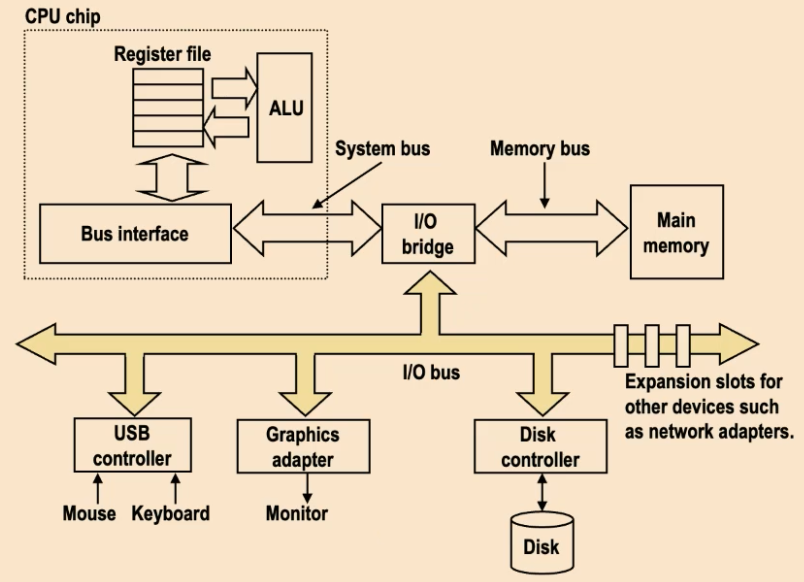
\includegraphics[scale=0.4]{img/io.png}
        \caption{Diagram of the IO bus.} 
        \label{fig:io}
      \end{figure}
    \end{definition}

    We can see from the diagram above that the CPU can directly access registers (since it's in the CPU itself) and the main memory (since it's connected to the memory bus). However, to access something like the disk, it must go through the disk controller. This gives us our first categorization of memory. 

    \begin{definition}[Primary Storage]
      \textbf{Primary storage devices} are directly accessible by the CPU and are used to store data that is currently being processed. This includes CPU registers, cache memory, and RAM. In memory, the basic storage unit is normally a \textbf{cell} (one bit per cell), which is the physical material that holds information. A \textbf{supercell} has address and data widths (number of bits), which is analogous to a lock number and the lock capacity, respectively. It is called random access since it takes approximately the same amount of time to access any cell in memory. There are two primary ways that this is implemented:  
      \begin{enumerate}
        \item \textbf{Static RAM (SRAM)} stores data in small electrical circuits (e.g. latches) and is typically the fastest type of memory. However, it is more expensive to build, consumers more power, and occupies more space, limiting the SRAM storage. 
        \item \textbf{Dynamic RAM (DRAM)} stores data using electrical components (e.g. capacitors) that hold an electrical charge. It is called \textit{dynamic} because a DRAM system must frequently refresh the charge of its capacitors to maintain a stored value. It also requires error correction which introduces redundancy. 
      \end{enumerate}

      \begin{table}[H]
        \centering
        \begin{tabular}{|l|l|l|l|}
        \hline
        \textbf{Device} & \textbf{Capacity} & \textbf{Approx. latency} & \textbf{RAM type} \\ \hline
        Register & 4 - 8 bytes & < 1 ns & SRAM \\ \hline
        CPU cache & 1 - 32 megabytes & 5 ns & SRAM \\ \hline
        Main memory & 4 - 64 gigabytes & 100 ns & DRAM \\ \hline
        \end{tabular}
        \caption{Memory hierarchy characteristics}
        \label{tab:memory_hierarchy}
      \end{table}
    \end{definition}

    \begin{definition}[Secondary Storage]
      \textbf{Secondary storage devices} are not directly accessible by the CPU and are used to store data that is not currently being processed. This includes hard drives, SSDs, and magnetic tapes. There are two primary ways: 
      \begin{enumerate}
        \item \textbf{Spinning disks} store data on a magnetic surface that spins at high speeds.
        \item \textbf{Solid state drives (SSDs)} store data on flash memory chips.
      \end{enumerate}
    \end{definition}

    There are three key components of memory that we should think about: 
    \begin{enumerate}
      \item The \textbf{capacity}, i.e. amount of data, it can store (how large the water tank is). 
      \item The \textbf{latency}, i.e. amount of time it takes for a device to respond with data after it has been instructed to perform a data retrieval operation (how fast the data flows). 
      \item The \textbf{transfer rate} or \textbf{thoroughput}, i.e. amount of data that can be moved between the device and main memory (how wide the pipe is). Naively, with one channel and sequential transfer the transfer rate is one over the latency. 
    \end{enumerate}

    We must provide a good balance of these three qualities, and also note that there are some physical limitations (i.e. latency cannot be faster than speed of light), and this is more effectively done through a hierarchical memory system.

    \begin{figure}[H]
      \centering 
      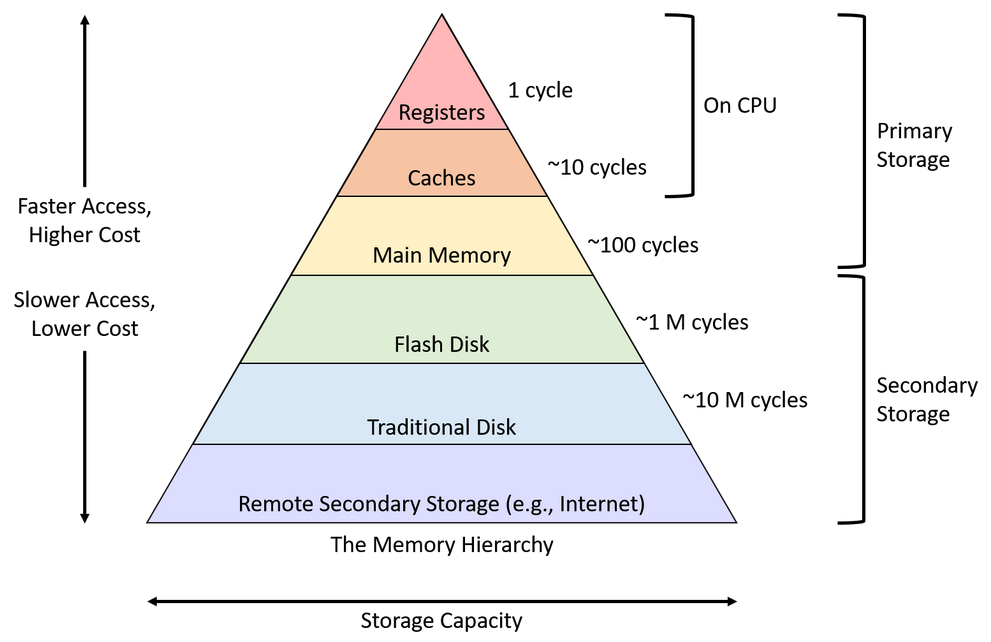
\includegraphics[scale=0.4]{img/memory_hierarchy.png}
      \caption{Memory hierarchy.} 
      \label{fig:memory_hierarchy}
    \end{figure}

    For example when we want to read from the disk, the CPU must request to the bus interface, which travels through the bus interface, I/O bridge, I/O bus, disk controller, and to the disk itself. Then the data goes back through the disk controller, I/O bus, I/O bridge, through the memory bus, and resides in the main memory. Note that disks are block addressed, so it will transfer the entire block of data into the memory. It must specify a \textbf{destination memory address (DMA)}. When the DMA completes, the disk controller notifies the CPU with an \textit{interrupt} (i.e. asserts a special interrupt pin on the CPU), letting it know that the operation has finished. This signal goes through the disk controller to the IO bridge to the CPU. From now on, the CPU knows that there is memory that it can access to run an application loaded in memory. 

  \subsection{Disk} 

    \begin{definition}[Hard Disk Drives]
      Back then, there were \textbf{hard disk drives (HDDs)} that literally had a spinning wheel and a needle head that read the data. 
      \begin{figure}[H]
        \centering 
        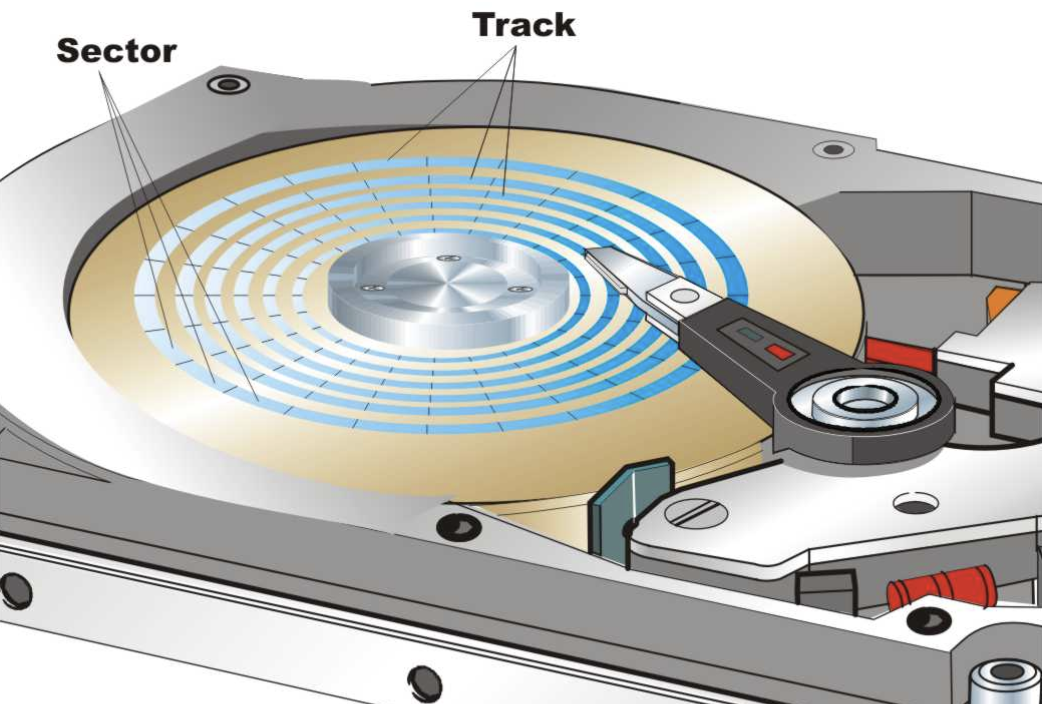
\includegraphics[scale=0.4]{img/hdd.png}
        \caption{Visual diagram of hard disk drive with its sectors. } 
        \label{fig:hdd}
      \end{figure}
      \begin{enumerate}
        \item HDDs are not random access since the data must be sequentially read. This was disadvantageous since the spinning wheel had to spin to the correct location, which took time. The needle also had to move to the correct location, which also took time and therefore read and write speeds were dominated by the time it took to move the needle.
        \item The smallest unit of data that can be read is a complete disk sector (not a single byte like RAM). 
      \end{enumerate}
    \end{definition}

    \begin{definition}[Solid State Drives]
      Now, we have \textbf{solid state drives (SSDs)} that store data on flash memory chips. This is advantageous since there are no moving parts, so the latency is much lower and the latency is not dominated by the time it takes to move the needle. 
      \begin{enumerate}
        \item SSDs are random access. 
        \item The smallest unit of data is a \textbf{page}, which is usually 4KB and maybe for high scale computers 2-4 MB (but on ``Big Data'' applications big but computers, it can be up to 1GB). 
        \item A collection of pages, usually 128 pages, is called a \textbf{block}, making is 512KB. 
      \end{enumerate}
    \end{definition}

    While virtually all RAM and primary storage devices are \textbf{byte addressable} (i.e. you can access any byte in memory), secondary storage devices are \textbf{block addressable} (i.e. you can only access a block of memory at a time). Therefore, to access a single byte in secondary storage, you must first load the entire block into memory, calculate which byte from that block you want, and then access it. Therefore, you need both the block number $x$ and the offset $o$ to access a byte in secondary storage, which is why it is even slower than accessing RAM. 

    \begin{figure}[H]
      \centering 
      \includegraphics[scale=0.4]{img/block_offset.png}
      \caption{Block offset.} 
      \label{fig:block_offset}
    \end{figure}

    Therefore, you can think of raw data in units of blocks of size $2^b$ for some $b$ bits. 
    \begin{enumerate}
      \item Take the low order $b$ bits of a byte address as an integer, which is the offset of the addressed byte in the block. 
      \item THe rest of the bits are the block number $x$, which is an unsigned long. 
      \item You request the block number $x$, receive the block contents, and then extract the requested byte at offset in $x$ i.e. calculate \texttt{block[x][offset]}. 
    \end{enumerate}

  \subsection{Locality}

    So far, we have abstracted away most of these memory types as a single entity with nearly instantaneous access, but in practice this is not the case. The most simple way is to simply have RAM and our CPU registers, but by introducing more intermediate memory types, we can achieve greater efficiency. 

    \begin{definition}[Locality]
      \textbf{Locality} is a principle that generally states that a program that accesses a memory location $n$ at time $t$ is likely to access memory location $n + \epsilon$ at time $t + \epsilon$. This principle motivates the design of efficient caches. 
      \begin{enumerate}
        \item \textbf{Temporal locality} is the idea that if you access a memory location, you are likely to access it again soon. 
        \item \textbf{Spatial locality} is the idea that if you access a memory location, you are likely to access nearby memory locations soon.
      \end{enumerate}
      This generally means that if you access some sort of memory, the values around that address is also likely to be accessed and therefore it is wise to store it closer to your CPU. In CPUs, both the instructions and the data are stored in the cache, which exploits both kinds of locality (repeated operations for temporal and nearby data for spatial). 
    \end{definition}

    \begin{example}[Locality]
      Consider the following code. 
      \begin{lstlisting}
        int sum_array(int *array, int len) {
          int i;
          int sum = 0;

          for (i = 0; i < len; i++) {
            sum += array[i];
          }

          return sum;
        }
      \end{lstlisting}
      \begin{enumerate}
        \item \textbf{Temporal Locality}
          \begin{enumerate}
            \item We cycle through each loop repeatedly with the same add operation, exploiting temporal locality.  
            \item The CPU accesses the same memory (stored in variables \texttt{i}, \texttt{len}, \texttt{sum}, \texttt{array}) within each iteration and therefore at similar times. 
          \end{enumerate}
        \item \textbf{Spatial Locality}
          \begin{enumerate}
            \item The spatial locality is exploited when the CPU accesses memory locations from each element of the array, which are contiguous in memory. 
            \item Even though the program accesses each array element only once, a modern system loads more than one \texttt{int} at a time from memory to the CPU cache. That is, accessing the first array index fills the cache with not only the first integer but also the next few integers after it too. Exactly how many additional integers get moved depends on the cache's \textbf{block size}. For example, a cache with a 16 byte block size will store \texttt{array[i]} and the elements in \texttt{i+1}, \texttt{i+2}, \texttt{i+3}. 
          \end{enumerate}
      \end{enumerate}
    \end{example}

    We can see the differences in spatial locality in the following example. 

    \begin{example}
      One may find that simply changing the order of loops can cause a significant speed up in your program. Consider the following code. 
      \begin{figure}[H]
        \centering 
        \noindent\begin{minipage}{.5\textwidth}
        \begin{lstlisting}[]{Code}
          float averageMat_v1(int **mat, int n) {
            int i, j, total = 0;

            for (i = 0; i < n; i++) {
              for (j = 0; j < n; j++) {
                // Note indexing: [i][j]
                total += mat[i][j];
              }
            }
            return (float) total / (n * n);
          }
        \end{lstlisting}
        \end{minipage}
        \hfill
        \begin{minipage}{.49\textwidth}
        \begin{lstlisting}[]{Output}
          float averageMat_v2(int **mat, int n) {
            int i, j, total = 0;

            for (j = 0; j < n; j++) {
              for (i = 0; i < n; i++) {
                total += mat[i][j];
              }
            }
            return (float) total / (n * n);
          }
          .
        \end{lstlisting}
        \end{minipage}
        \caption{Two implementations of taking the total sum of all elements in a matrix.} 
        \label{fig:matrix_sum}
      \end{figure}
      It turns out that the left hand side of the code executes about 5 times faster than the second version. Consider why. When we iterate through the \texttt{i} first and then the \texttt{j}, we access the values \texttt{array[i][j]} and then by spatial locality, the next few values in the array, which are \texttt{array[i][j+1]}, ... are stored in the cache. 
      \begin{enumerate}
        \item In the left hand side of the code, these next stored values are exactly what is being accessed, and the CPU can access them in the cache rather than having to go into memory. 
        \item In the right hand side of the code, these next values are \textit{not} being accessed since we want to access \texttt{array[i+1][j]}, .... Unfortunately, this is not stored in the cache and so for every $n^2$ loops we have to go back to the memory to retrieve it. 
      \end{enumerate}
    \end{example}

  \subsection{Caches}

      In theory, a cache should know which subsets of a program's memory it should hold, when it should copy a subset of a program's data from main memory to the cache (or vice versa), and how it can determine whether a program's data is present in the cache. Let's talk about the third point first. It all starts off with a CPU requesting some memory address, and we want to determine whether it is in the cache or not. To do this, we need to look a little deeper into memory addresses. 

      \begin{definition}[Portions of Memory Addresses]
        A memory address is a $m$-bit number.\footnote{64 in 64-bit machines.} It is divided up into three portions. 
        \begin{enumerate}
          \item The \textbf{tag} field with $t$ bits at the beginning.
          \item The \textbf{index} field with $i$ bits in the middle. 
          \item The \textbf{offset} field with $o$ bits at the end.
        \end{enumerate}
        The tag plus the index together refers to the \textbf{block number}. 
        \begin{figure}[H]
          \centering 
          \includegraphics[scale=0.4]{img/memory_portions.png}
          \caption{Portions of a 16 bit memory address with $t = 4, i = 7, o = 5$. } 
          \label{fig:memory_portions}
        \end{figure}
      \end{definition}

      Before we see why we do this, we should also define the portions of a CPU. 

      \begin{definition}[CPU Cache]
        A \textbf{CPU cache} divides its storage space as follows. A cache is essentially an array of sets, where $S$ is the number of sets. Each set is divided into $E$ units called \textbf{cache lines/rows}, with each cache line independent of all others and contains two important types of information. 
        \begin{enumerate}
          \item The \textbf{cache block} stores a subset of program data from main memory, of size $2^o$.\footnote{In Intel computers, it is typically 64 bytes long and for Mac Silicon, it is 128 bytes.} Sometimes, the block is referred to as the cache line. Note that is the cache block size is $2^o$ bytes, then the block offset field has length $\log_2 2^o = o$.
          \item The \textbf{metadata} stores the \textbf{valid bit} (which tells us if the actual data in memory is valid), and the \textbf{tag} of length $t$ (the same as the tag length of the memory address) which tells us the memory address of the data in the cache. 
        \end{enumerate}
        Therefore, the \textbf{cache size} is defined to be $C = S \cdot E \cdot B$ (the metadata is not included). 
        \begin{figure}[H]
          \centering 
          \includegraphics[scale=0.4]{img/direct_mapped_cache.png}
          \caption{Diagram of a direct-mapped cache.} 
          \label{fig:direct_mapped_cache}
        \end{figure}
        CPU caches are built-in fast memory (SRAM) that stores stuff. There are two types: 
        \begin{enumerate}
          \item \textbf{i-cache} stores copies of instructions. 
          \item \textbf{d-cache} stores copies of data from commonly referenced locations. 
        \end{enumerate}
        We saw that caches come in different levels, they all just hold words retrieved from a higher level of memory. 
        \begin{enumerate}
          \item CPU registers hold words retrieved from L1 cache. 
          \item L1 holds cache lines retrieved from L2 cache. 
          \item L2 cache holds cache lines retrieved from L3 cache or the main memory.  
          \item Main memory holds disk blocks retrieved from local disks. 
          \item Local disks hold blocks retrieved from remote disks or network servers. 
        \end{enumerate}

        \begin{figure}[H]
          \centering 
          \includegraphics[scale=0.4]{img/cache_retrieve.png}
          \caption{How caches retrieve data from higher levels of memory.} 
          \label{fig:cache_retrieve}
        \end{figure}
      \end{definition}

      \begin{example}[Simple Calculations]
        Given a direct-mapped cache specified by a block size of 8 bytes and a cache capacity of 4 KB, 
        \begin{enumerate}
          \item the cache can hold 512 blocks. 
          \item the block offset field is $\log_2 8 = 3$ bits wide. 
          \item the address \texttt{0x1F = 0b00011111} is in block number $3$ since the last three bits are the offset, and whatever is left (passed through the hashamp, which is simply modulo), is the block number. 
        \end{enumerate}
      \end{example}

      In \textbf{I/O caches}, software keeps copies of cached items in memory, indexed by name via a hash table.

      At the lowest level, registers are explicitly program-controlled, but when accessing any sort of higher memory, the CPU doesn't know whether some data is in the cache, memory, or the disk. 

      \begin{figure}[H]
        \centering 
        \includegraphics[scale=0.4]{img/hierarchy2.png}
        \caption{} 
        \label{fig:hierarchy2}
      \end{figure}

      Finally, let's compare software vs hardware caches. 

      \begin{definition}[Software Caches]
        When implementing caches in software, there are large time differences (DRAM vs disk, local vs remote), and they can be tailored to specific uses cases. They also have flexible and sophisticated approaches with data structures (like trees) and can perform complex computation. 
      \end{definition}

      Theoretically, when implementing hash tables, you never actually have to evict something. You can have the values of the table to be a linked list where we add to the head. If there is unlimited chaining, we have a full associative cache, and if we have limited chaining (e.g. 5), it is like a 5-way set associative cache. If it goes out of bound, we can implement LRU by removing the tail of the linked list. 

      \begin{definition}[Hardware Caches]
        In hardware caches, there are smaller time differences, needs to be as fast as possible, and parallelization is emphasized. 
      \end{definition}

      There are slightly different implementations of caching, and for each implementation, we will describe 
      \begin{enumerate}
        \item how to load data from memory into the cache, 
        \item how to retrieve data from the cache, 
        \item how to write data to the cache. 
      \end{enumerate}

    \subsubsection{Direct Mapped Cache} 

      A direct mapped cache is a caching implementation when we assume that $E = 1$, which means that for any given memory address, there is only one possible cache line that can store this data at that memory address. That is, the cache is really just a bunch of sets with one cache line each, and each cache line is completely isolated from the others. Whether we load data from memory into cache or try to retrieve data from the cache, it's really the same process. 

      \begin{theorem}[Placement]
        To load data from memory into the cache, which happens when there is a \textbf{cache miss}, we do the following. 
        \begin{enumerate}
          \item The CPU requests a memory address $M = (T, I, O)$. 
          \item There exists a hashmap $H$ that maps the index $I$ to a cache line. 
          \item At line $H(I)$, we can get a cache miss and must load from memory into this cache. 
          \item We wait until the memory has retrieved the data from the portion of the memory. i.e. we wait for the $2^o$ bytes located at addresses $(T, I, 0\ldots 0)$ to $(T, I, 1\ldots 1)$. Call this data $D$. 
          \item The $2^o$ byte string $D$ is stored in the cache data block at line $M(I)$,ready to be used. 
        \end{enumerate}
      \end{theorem}

      \begin{theorem}[Lookup]
        To see whether a requested memory address is in the cache, we do the following. 
        \begin{enumerate}
          \item The CPU requests a memory address $M = (T, I, O)$. 
          \item There exists a hashmap $H$ that maps the index $I$ to a cache line. 
          \item At line $H(I)$, check the cache line's valid bit. If it is not valid, then this is a cache miss and we must go to the memory to retrieve the data, leading to the above process. 
          \item Since there could be multiple $I$ that maps to the same cache line, there will be overlap. But this is where the tag portion comes in. At cache line $H(I)$, the CPU checks the cache tag to see if it matches the memory tag $T$. 
          \item If it does, then we have just found a way to identify the first $t + i$ bits of the requested memory address, and we have gotten a cache hit. Now, we know that the cache's data block holds the data that the program is looking for. We use the low-order offset bits of the address to extract the program's desired data from the stored block. 
        \end{enumerate}
        \begin{figure}[H]
          \centering 
          \includegraphics[scale=0.4]{img/cache_request.png}
          \caption{Diagram of a cache request. Note that since the entire data in the memory block stored in the cache, we can take advantage of spatial locality.}  
          \label{fig:cache_request}
        \end{figure}
      \end{theorem}

      So far, we've talked about reading operations, but what about writing to the cache? It is generally implemented in two ways. 

      \begin{definition}[Write-Through, Write-Back Cache]
        Note that when we write data to cache, it does not need to be immediately written to memory, but rather it can be flushed to memory at a later time. This is efficient since if we have repeated operations on a single memory address, we don't have to go back and forth between the CPU and memory. 
        \begin{enumerate}
          \item In a \textbf{write-through cache}, a memory write operation modifies the value in the cache and simultaneously writes the value to the corresponding location in memory. It is always synchronized. 
          \item In a \textbf{write-back cache}, a memory write operation modifies the value stored in the cache's data block, but does \textit{not} update main memory. Instead, the cache sets a \textbf{dirty bit} in the metadata to indicate that the cache block has been modified. The modified block is only written back to memory when the block is replaced in the cache. 

          \begin{figure}[H]
            \centering 
            \includegraphics[scale=0.4]{img/dirty_bit.png}
            \caption{A dirty bit is a one bit flag that indicates whether the data stored in a cache line has been modified. When set, the data in the cache line is out o sync with main memory and must be written back (flushed) back to memory before eviction. } 
            \label{fig:dirty_bit}
          \end{figure}
        \end{enumerate}
        As usual, the difference between the designs reveals a trade-off. Write-through caches are less complex than write-back caches, and they avoid storing extra metadata in the form of a dirty bit for each line. On the other hand, write-back caches reduce the cost of repeated writes to the same location in memory.
      \end{definition}

      \begin{theorem}[Replacement]
        Replacement occurs exactly the same way as if we just did a placement and is trivial. We retrieve the data block from the memory and store it in the cache. Direct-mapping conveniently determines which cache line to evict when loading new data. Given new memory $M = (T, I, O)$, you \textit{must} evict the cache line at $H(I)$. 
      \end{theorem}

    \subsubsection{N way Set-Associative Cache}

      Note that for both examples, given a fixed hashmap $H$ it is not possible to store data in two memory addresses $M_1$ and $M_2$ where both $H(I_1) = H(I_2)$. Therefore, the choice of hashing must be done so that it minimizes the number of collisions. So far, we have only considered memory read operations for which a CPU performs lookups on the cache. Caches must also allows programs to store values. However, there is a better way to do this: just construct it so that each set has more than one cache line, and so data in index portions of different memory addresses can be stored in different cache lines.

      In here, we deal with $E \neq 1$, and so there are multiple set each with multiple lines. This means that the cache is more like a 2D array, and when we want to retrieve an index, we must look through the $H(I)$th line in \textit{each} set to see if the tag matches. 

      \begin{theorem}[Lookup]
        To see whether a requested memory address is in the cache, we do the following. 
        \begin{enumerate}
          \item The CPU requests a memory address $M = (T, I, O)$. 
          \item We iterate through each of the $S$ sets in the cache, looking at cache line $M(I)$. 
          \item For each line, we check if it is valid and if so, whether the line tag matches the memory tag. If we get a hit, then we have found the data in the cache. 
        \end{enumerate}
        \begin{figure}[H]
          \centering 
          \includegraphics[scale=0.4]{img/retrieve_set_associative.png}
          \caption{Diagram of a 2 set-associative cache.} 
          \label{fig:retrieve_set_associative}
        \end{figure}
      \end{theorem}

      If you have a \textbf{fully associative cache}, then you have one set with $E = C/B$ lines. Therefore, you can really put any memory address data in any cache line. There is a clear tradeoff here. As we increase $N$, we can get more flexibility in using all of our cache space, but the time complexity of retrieving and writing data scales linearly. In fact, this linear scan is too slow for a cache, which is why you need to implement some parallel tag search, but this turns out to be quite expensive to build.\footnote{You have to copy the request tag with a circuit and compare it to all the tags in the cache, which turns out to be a much larger circuit.}
    
      Though we have a more robust implementation with associative mapping, placement and replacement now face the problem of \textit{which} set to place the data in or evict existing data. 

      \begin{theorem}[Placement]
        To load data from memory into the cache this is trivial since we can just go through the sets, find one where the valid bit is $0$, and just place the data there.  
      \end{theorem}

      In replacement, this is a bit trickier, but using the principle of temporal locality, we can try and replace the least recently used cache. This tries to minimize cache misses, but not slow down the lookup too much. 

      \begin{theorem}[Replacement]
        To replace data on the cache, we use the \textbf{least recently used (LRU)} algorithm. This matches temporal locality, but it also requires some additional state to be kept. 
      \end{theorem}

    \subsubsection{Types of Cache Misses} 

      There are three types of cache misses. 

      \begin{definition}[Cold (Compulsory) Miss]
        A \textbf{cold miss} occurs when the cache is empty and the CPU requests a memory address. This is the first time the CPU is requesting this memory address, and so it must go to the memory to retrieve the data.
      \end{definition}
      
      \begin{definition}[Capacity Miss]
        A \textbf{capacity miss} occurs when the cache is full and the CPU requests a memory address that is not in the cache. This is because the cache is full and so the CPU must evict some data to make space for the new data.
      \end{definition}

      \begin{definition}[Conflict Miss]
        A \textbf{conflict miss} occurs from premature eviction of a warm block. 
      \end{definition}

    Valgrind's cachegrind mode. 

\section{Operating Systems}

    Up until now, we've seen the dynamics of how one program works in a computer system. The code, which first resides in the disk, is fetched (through blocks) into memory, and after compiling (precomiling, compiling, assembling, linking), we have a binary. The binary is then loaded into memory in the stack frame, and the CPU executes the instructions. The CPU also has a cache, which stores the most frequently accessed data during the process, taking advantage of locality for efficiency. 

    Our computer obvious does not just run one program. It runs several, and to run several, we need some control mechanism to manage how these programs interact with the CPU, memory, and disk. For example, one problem is that if we download application A and application B and run their binaries, how do we know whether they share memory addresses and consequently overwrite each other's data?\footnote{This is different from linking, where we have relocation tables to ensure that \textit{object files} do not conflict with each other.} The operating system takes care of these, which manages \textit{processes} that each have their own \textit{virtual memory space}. 

    Furthermore, consider some of the components of the computer: the RAM, disk, and IO devices like your keyboard and monitor. For security reasons, it is not wise to let the user applications (e.g. Chrome or Slack) control these devices completely. Their power must be restricted in some way. 
    \begin{enumerate}
      \item When you have a Chrome window and resize it, Chrome should not be able to modify the pixels outside that window. 
      \item When you want to print some statement using \texttt{printf}, 
      \item When you're editing a code file with VSCode, you want to limit the application to save to certain parts of the disk. 
      \item When you are running Chrome and Slack together, you don't want them to read each other's data directly. 
    \end{enumerate}
    This is also for convenience. Say that if you are creating an application that has the option to save files to disk, you don't want to write the hardware backend to write to the disk. You want to just call a function that writes to the disk, and the OS will take care of the rest. 

    \begin{definition}[Operating System]
      A common confusion is that people think that the \textbf{operating system} describes the computer itself, but it is really just another piece of software. What makes this piece of software so special is that it manages every other software in the computer. It provides generally three services: 
      \begin{enumerate}
        \item It \textbf{multiplexes} the hardware resources. Since there are many applications/programs with finite CPU resources (number of cores) and shared access to storage devices, the OS schedules some sharing mechanism for execution time on CPU cores and manages access to storage devices.
        \item It \textbf{abstracts} the hardware platform. Since each CPU core simply executes a sequence of instructions, the OS introduces processes and thread abstractions. Furthermore, it introduces \textit{filesystems} (file/directories) on top of raw storage devices. 
        \item It \textbf{protects} software principals from each other. Since many applications from various users are using the CPU, the OS provides isolation between them. It enforces user access permission (read/write) for files. 
      \end{enumerate}
    \end{definition}

    The OS is booted by the system firmware (BIOS or UEFI), which lives in ROM (sRAM and therefore non-volatile) and copies the OS from a fixed part of the disk, called the \textbf{bootloader}, into the RAM, which itself then loads the OS into memory. Once the OS starts running, it loads the rest of itself from disk, discovers and initializes hardware resources, and initializes its data structures and abstractions to make the system ready for users.

    \begin{definition}[Kernel]
      The \textbf{kernel} is the actual binary that is loaded into RAM that runs the OS. The kernel code and data resides in a fixed and protected range of addresses, called the \textbf{kernel space}, and user programs cannot access kernel space. 
    \end{definition}

  \subsection{Control Flow}

    When we worked with jumps (conditional and unconditional), calls, and returns in assmebly, all of these operations were with respect to the \textbf{program state}, which is the isolated environment that the program is in. One program doesn't have any clue of what is going on anywhere else, such as other programs or input/output signals. This means that given what we have learned, 
    \begin{enumerate}
      \item programs cannot to write files to the disk (since that is outside the program). 
      \item programs cannot be terminated by pressing \texttt{CTRL + C} on the keyboard. 
      \item programs cannot receive data that arrives from the disk. 
      \item programs cannot send data to the monitor to display. 
      \item programs cannot react accordingly when there is an instruction to divide by $0$.\footnote{I guess you can use a conditional jump to check if the divisor is $0$ and then jump to a different part of the code.}
    \end{enumerate}
    To do all these things, we need to have access to the global \textbf{system state}, which the OS has access to. 

    It turns out that it is impossible for jumps and procedure calls to achieve this, and rather the system needs mechanisms for \textbf{exceptional control flow} (i.e. control flow that is not within the regular program state), or commonly referred to as \textbf{exceptions}. This requires the CPU to enter into a more powerful state than its current place in the program state, called the kernel state. The actual thing that triggers this is called an \textbf{interrupt}, which can come from both the hardware and software. In the kernel state, the CPU can access the hardware and perform operations that the program state cannot to handle these exceptions. 

    \begin{example}[Interrupts]
      Some examples of how the OS can be interrupted is: 
      \begin{enumerate}
        \item when one's WiFi card detects a signal. 
        \item a hard disk drive may interrupt the OS if a read fails due to a bad sector. 
        \item an application may request a system call to open a file. 
        \item If you have 10 applications running on 1 CPU core, you may want the CPU core to run to the next application every 10 milliseconds. So, there may be a system call every 10 milliseconds in each program to the OS to switch to the next application. 
      \end{enumerate}
    \end{example}

    \begin{definition}[Execution Modes]
      The CPU helps with this by providing two execution modes, which is determined by a special bit in the CPU called the \textbf{mode bit}. 
      \begin{enumerate}
        \item In \textbf{user mode}, the CPU executes only user-level instructions and accesses only the memory locations that the OS makes available to it. It also restricts which hardware components the CPU can directly access. 
        \item In \textbf{kernel mode}, the CPU executes any instructions and accesses any memory location (including those that store OS instructions and data). It can also directly access hardware components and execute special instructions. 
      \end{enumerate}
      Note that the execution mode is \textit{property of the CPU}!  
    \end{definition}

    \begin{example}[Monitor]
      A monitor is really just some device that scans a certain portion of memory at a certain frequency that is higher than the human eye can detect. In user mode, if you try to access this memory buffer, you get an exception. No user mode can access this memory buffer. 
    \end{example}

    \begin{example}[Amazon.com]
      When you are on Amazon to search up some product, you want to type in some keyword in the search bar. The web browser, say Chrome, that you are running it on, runs in user mode. When you type in the keyword, Chrome sends a system call to the OS, triggering the kernel mode which retrieves the keys that you pressed, and redirects it to Chrome. The same goes with the location of your mouse. When you move and click on a product, Chrome sends a system call to the OS, which then receives the mouse location and sends it back to Chrome. The application has no way to directly access the hardware. 
    \end{example}

    Now specifically, how does one enter in this kernel mode? We've already hinted at it before, but to elaborate, there are 4 types of exceptions. 

    \begin{definition}[Types of Exceptions/Interrupts]
      As we have mentioned, we go into kernel mode through exceptional control flows. To go back from the kernel mode to the user mode after the exception handling is done, the kernel must explicitly give back the control to the user program, which is done with a special instruction, which changes the CPU to the user mode again. At this point, it can return back to user mode at the current instruction, next instruction, or abort it. 
      \begin{enumerate}
        \item These control flows can either by \textbf{synchronous} (caused by an instruction) or \textbf{asynchronous} (caused by some other event external to the processor). Asynchronous interrupts are indicated by setting the processor's interrupt pins. 
        \item Furthermore, \textbf{intentional} exceptions transfer control to the OS to perform some function, and \textbf{unintentional} exceptions happen when there is a bug. 
      \end{enumerate}
      This gives us 4 categories of exceptions. 
      \begin{enumerate}
        \item Intentional synchronous exceptions are \textbf{system calls}, aka \textbf{traps} (e.g. \texttt{printf}, \texttt{open}, \texttt{close}, \texttt{write}, breakpoint traps, special instructions). It returns control to the next instruction. 
        \item Unintentional synchronous exceptions are \textbf{faults} (possibly recoverable) or \textbf{aborts} (unrecoverable) (e.g. invalid or protected address or opcode, page fault, overflow, divide by zero). This automatically triggers the kernel mode which then uses an exception handler to kill the process.  
        \item Intentional asynchronous exceptions are \textbf{software interrupts}, which is when software requests an interrupt to be delivered at a later time (e.g. there's some task you want the kernel to do later). 
        \item Unintentional asynchronous exceptions are \textbf{hardware interrupts} caused by an external event (e.g. IO such as \texttt{CTRL + C}, op completed, timers which may switch to another application every 10ms, power fail, keyboard, mouse click, disk, receiving a network packet). Unlike system calls, which come from executing program instructions, hardware interrupts are delivered to the CPU on an \textbf{interrupt bus}. 
      \end{enumerate}
      Once a system call or hardware interrupt is finished, the program continues to resume back in user mode. 
      \begin{figure}[H]
        \centering 
        \includegraphics[scale=0.4]{img/interrupt.png}
        \caption{The CPU and interrupts. User code running on the CPU is interrupted (at time X on the time line), and OS interrupt handler code runs. After the OS is done handling the interrupt, user code execution is resumed (at time Y on the time line).} 
        \label{fig:interrupt}
      \end{figure}
    \end{definition}

    Now the question arises: how does the CPU know where to go when an system call or interrupt occurs? These are done through tables that map some unique ID number to some functionality. These tables are stored in a protected memory space reserved by the kernel. 

    \begin{definition}[System Call Table]
      This is done through the \textbf{system call table}, which is a table of addresses in memory that the CPU can jump to when a system call occurs. Each system call has a unique number $k$, and the handler function $k$ is called each time system call $k$ occurs. 
    \end{definition}

    \begin{example}[Common System Calls]
      Some common system calls, or \textbf{syscalls}, are shown below with their unique ID number (in Linux x64). 
      \begin{table}[H]
        \centering
        \caption{System Call Functions}
        \begin{tabular}{|c|l|l|}
        \hline
        \textbf{Number} & \textbf{Name} & \textbf{Description} \\ \hline
        0 & read & Read file \\ \hline
        1 & write & Write file \\ \hline
        2 & open & Open file \\ \hline
        3 & close & Close file \\ \hline
        4 & stat & Get info about file \\ \hline
        57 & fork & Create process \\ \hline
        59 & execve & Execute a program \\ \hline
        60 & \_exit & Terminate process \\ \hline
        62 & kill & Send signal to process \\ \hline
        \end{tabular}
      \end{table}
    \end{example}

    \begin{example}[Syscalls of Open] 
      Look at the following objdump file below. The corresponding C code just calls \texttt{open(filename, options)} and the corresponding syscall ID is \texttt{0x2}. We are simply loading the syscall ID into the \texttt{\%eax} register (only needs last 32 bits since the syscall IDs are quite small), which is then executed by the \texttt{syscall} instruction to go into the kernel mode. 
      \begin{lstlisting}
        00000000000e5d70 <__open>: 
        ...
        e5d79:  b8 02 00 00 00       mov    $0x2,%eax     # 2 is the open syscall number
        e5d7e:  0f 05                syscall              # return value in %rax
        e5d80:  48 3d 01 f0 ff ff   cmp    $0xfffffffffffff001,%rax 
        ... 
      \end{lstlisting}
      A negative number in \texttt{\%eax} gives an error corresponding to negative \texttt{errorno}. It is also worth mentioning that \texttt{\%eax} is used rather than \texttt{\%rdi} or \texttt{\%rsi} because we need these two parameter registers as arguments for the \texttt{open} function itself. 
    \end{example}

    Note that whether we are in the program stack or the kernel stack, we always have stack pointers and other registers to navigate them. In fact, for every CPU core, it has its own set of registers and its own kernel stack. 

    \begin{example}[Syscall of Read]
      If we have read syscall, then 
      \begin{enumerate}
        \item We use the syscall table to go to the trap handler for the read syscall. 
        \item The handler identifies the block and allocates a buffer. 
        \item Then it reads the block from the disk, which may take a while (in CPU time) since it is extremely slow for all IO tasks. The CPU, while waiting, can be put to sleep for other processes to run on the CPU. When the disk is done reading, it (the hardware) can send a hardware interrupt to the CPU, telling it that it is done. 
        \item Then it copies the block to the user buffer and returns from the syscall back into the user mode in the program state. 
      \end{enumerate}
    \end{example}

    \begin{definition}[Exception Table]
      This is done through the \textbf{exception table}, which is a table of addresses in memory that the CPU can jump to when an exception occurs. Each type of event has a unique exception number $k$, and the handler function $k$ is called each time exception $k$ occurs.\footnote{This is similar to a hardware implementation of a switch statement in C.}
      \begin{figure}[H]
        \centering 
        \includegraphics[scale=0.4]{img/exception_table.png}
        \caption{System call table is stored in a protected memory space reserved by the kernel.} 
        \label{fig:system_call_table}
      \end{figure}
    \end{definition}

    \begin{example}[Common Exception Numbers]
      Some common exception numbers are listed below. 
      \begin{table}[H]
        \centering
        \caption{Exception Summary}
        \begin{tabular}{|c|l|l|}
        \hline
        \textbf{Exception Number} & \textbf{Description} & \textbf{Exception Class} \\ \hline
        0 & Divide Error & Fault \\ \hline
        13 & General protection fault & Fault \\ \hline
        14 & Page fault & Fault \\ \hline
        18 & Machine check & Abort \\ \hline
        32-255 & OS-defined & Interrupt or trap \\ \hline
        \end{tabular}
      \end{table}
    \end{example}

    From the application's point of view, even if an interrupt happens, it just thinks it is running line by line. 

    \begin{definition}[Process Address Space]
      Interrupts can happen at any time, and one way to efficiently support this execution context switch from user mode to kernel mode is to do the following. At boot time, the OS loads its kernel code at a fixed location in RAM. Every time you create a new program state, the OS initializes a CPU register with the starting address of the OS handler function. On an interrupt, the CPU switches to kernel mode and executes OS interrupt handler code instructions that are accessible at the top addresses in every process’s address space. Because every process has the OS mapped to the same location at the top of its address space, the OS interrupt handler code is able to execute quickly in the context of any process that is running on the CPU when an interrupt occurs. This OS code can be accessed only in kernel mode, protecting the OS from user-mode accesses; during regular execution a process runs in user mode and cannot read or write to the OS addresses mapped into the top of its address space.\footnote{However, due to security reasons where the user space can read kernel space data, this is obsolete.}

      \begin{figure}[H]
        \centering 
        \includegraphics[scale=0.4]{img/process_address_space.png}
        \caption{Process address space: the OS kernel is mapped into the top of every process’s address space.} 
        \label{fig:process_address_space}
      \end{figure}
    \end{definition}

    In summary, a good visual is that each program runs as independent processes, with its own virtual address space (elaborated next) and the OS mediates access to shared resources.  

    \begin{figure}[H]
      \centering 
      \includegraphics[scale=0.3]{img/os_multiple_programs.png}
      \caption{Multiple programs running and controlled by an operating system.} 
      \label{fig:os_multiple_programs}
    \end{figure}

    Each process can be in one of three states. It can either be currently running on the state, ready to run, or if there is a long IO operation, it can be blocked, which is then unblocked with a hardware interrupt. Usually anything that involves IO puts the state to blocked (e.g. reading data from disk, the keyboard, or the internet). The pool of processes that are concurrently running is the running and ready states. 
    \begin{figure}[H]
      \centering 
      \includegraphics[scale=0.4]{img/3_process_states.png}
      \caption{Three states that a single process can be in. The pool of processes that are concurrently running is the running and ready states. The blocked state is waiting to be put back into this pool by a hardware interrupt.} 
      \label{fig:3_process_states}
    \end{figure}

    \begin{example}[Running a Binary]
      Therefore, to run a binary file \texttt{a.out}, 
      \begin{enumerate}
        \item The kernel first loads the binary file from disk into RAM.
        \item Then the OS kernel creates a new process with its own virtual memory stack and its global variables, etc. 
        \item Then the CPU's \texttt{\%rip} register point to the address of the \texttt{main} function. 
        \item The kernel's virtual memory space is mapped to the top of the process's virtual memory space, where it is not visible to the user mode. 
      \end{enumerate}
      \begin{figure}[H]
        \centering 
        \includegraphics[scale=0.4]{img/process_space.png}
        \caption{The kernel's virtual memory space is mapped to the top of the process's virtual memory space.} 
        \label{fig:process_space}
      \end{figure}
    \end{example}

  \subsection{Virtual Memory}

    We have mentioned that there is a problem where two different application developers, who have linked their own C files to create binaries, can be installed on one computer and run at the same time. However, the linking has already been finished and the memory addresses of the symbols in each executable are fixed. This can be a problem if there are overlaps in the memory addresses. 

    \begin{definition}[Virtual Memory]
      The actual main memory of our system is referred to as the \textbf{physical memory}. To prevent such overlaps, the kernel and each user process has its own \textbf{virtual memory}. That is, there exists a \textbf{memory management unit (MMU)} in the CPU that translates virtual addresses to physical addresses through a hashmap. 
      \begin{figure}[H]
        \centering 
        \includegraphics[scale=0.4]{img/mmu.png}
        \caption{Memory management unit maps each virtual address to a physical address.} 
        \label{fig:mmu}
      \end{figure}
      This allows the kernel to map the virtual memory of each process to the physical memory.
      \begin{figure}[H]
        \centering 
        \includegraphics[scale=0.4]{img/vm_map.png}
        \caption{Each process has its own virtual memory space, which is mapped by the MMU to the physical memory space. } 
        \label{fig:vm_map}
      \end{figure}
    \end{definition}

    \begin{example}[Virtual and Physical Memory Size]
      Given a $n$-bit machine with $2^m$-bytes of memory, $n > m$ and so there are more virtual addresses than physical addresses. If we have a 64-bit machine with 16GB of memory, then there are $2^{64}$ virtual addresses and $2^{3} \cdot 2^{34} = 2^{37}$ bits of physical memory. If there are 8 processes running then there are $8 \cdot 2^{64} = 2^{67}$ bits of virtual memory. 
    \end{example}

    There are many properties of virtual memory that solves a lot of problems and makes things more convenient. The main property is called \textbf{indirection} which means that the virtual memory is not the actual physical memory. 
    \begin{enumerate}
      \item The first problem is that there are much more virtual addresses than physical addresses. Even storing a table for one process would take up more than all of your RAM. Therefore, for every byte in main memory, there exists one physical address (PA) and zero, one, or more virtual addresses (VA). We will elaborate on the specifics of this implementation later. 
      \item We also need to have memory management. Every process has its own stack, heap, \texttt{.text}, and \texttt{.data} sections. We must be able to allocate and deallocate memory and fit this accordingly. 
      \item We also need to have protection. We need to ensure that one process cannot read or write to another process's memory.
      \item While we want isolation, we also want sharing between processes if needed (e.g. signing into Slack using Google on a browser). Furthermore, if there are multiple calls of the \texttt{printf} function, we can just have a single copy of the \texttt{printf} function in memory rather than having multiple copies for each process. This can be done through the concept of permissions. 
    \end{enumerate}

    Let's talk about how we should actually map these addresses. One property of this mapping is that we want contiguous addresses both in the virtual and the physical level so that we can store arrays, exploit locality, etc. Therefore, we can use larger blocks known as \textit{pages}. Just like how we have divided memory addresses into sections that can be used to map to caches, we can divide the memory addresses into sections that can be used to map to the physical memory. Note that this also takes care of the first problem partially since now we can fit this table in the memory. 
      
    \begin{definition}[Page]
      Both in virtual and physical memory, an $n$-bit address can be divided into a \textbf{page number} and an \textbf{offset}. The page number is $n - 12$ and the offset is $12$ bits. The page number is used to index into a \textbf{page table} that maps the page number to a physical address. 
      \begin{figure}[H]
        \centering 
        \includegraphics[scale=0.4]{img/page.png}
        \caption{A page is a contiguous block of memory addresses.} 
        \label{fig:page}
      \end{figure}
      While the entire page table is stored in memory (at memory stored by a protected CPU register), a portion of the page table is stored in the CPU cache. 
      \begin{enumerate}
        \item The virtual page number (VPN) is equivalent to the block number. 
        \item The page offset is equivalent to the block offset. 
      \end{enumerate}
    \end{definition}

    \begin{example}[Page Number]
      In a 64-bit machine with 16GB of RAM, you have $2^{64} / 2^{12} = 2^{52}$ virtual pages and $2^{37} / 2^{12} = 2^{25}$ physical pages. 
    \end{example}

    Therefore, our translation table is really a map from a virtual page number to a physical page number, rather than a virtual address to a physical address. This is created at runtime. Therefore, 
    \begin{enumerate}
      \item The virtual page number $VP$ is mapped through some map $M$ to get the physical page number $PP$. 
      \item The virtual offset is the same as the physical offset. 
    \end{enumerate}

    \begin{definition}[Page Table]
      The \textbf{page table} is a hashmap that maps the virtual page number to the physical page number defined as the mapping 
      \begin{equation}
        H: \underbrace{(VP,m)}_{\text{64 bits}} \longrightarrow PP
      \end{equation}
      Each input-output pair is called a \textbf{page table entry (PTE)}, and virtual memory is \textbf{fully associative}, meaning that any virtual page can be placed in any physical page, though it requires a large mapping function (the PT), which is different from CPU caches. 
      \begin{figure}[H]
        \centering 
        \includegraphics[scale=0.4]{img/page_table.png}
        \caption{The page table only needs the virtual page number plus the metadata to map to the physical page number. The offset is provided by the virtual memory address itself. } 
        \label{fig:page_table}
      \end{figure}
      Note that while we want to store the 52-bit VP in the page table, the actual input is still 64-bits, with 12 bits of metadata $m$. This metadata contains some information about the following 
      \begin{enumerate}
        \item A bit that indicates whether the page is a read, write, or executable piece of code (3 bits). 
        \item A bit that indicates whether the page is valid or not. 
      \end{enumerate}
      \begin{figure}[H]
        \centering 
        \includegraphics[scale=0.4]{img/permissions_vm.png}
        \caption{The page table entry contains the physical page number and some metadata.} 
        \label{fig:permissions_vm}
      \end{figure}
    \end{definition}

    Therefore, if you malloc, you are really just allocating some virtual memory addresses, which then get mapped to physical memory addresses in one or more pages. 

    \begin{definition}[Page Fault]
      It is clear that not every virtual page number can be mapped to a physical page number. If it turns out that a \textbf{page fault} happens if 
      \begin{enumerate}
        \item the virtual page number maps to no physical page (i.e. is not in the page table) in the RAM
        \item if some user program tries to access a physical page owned by the kernel
        \item if the page number maps to some place in the disk (but it is not in physical RAM)
      \end{enumerate}
      Page faults can be used in a lot of creative ways, but to reduce the risk of a page fault, e.g. when running out of physical memory, we can move some physical pages into disk and allocate memory by creating a new entry in our page table that maps this application's virtual page into the now empty physical page. 
    \end{definition}

    Note that by this construction, instructions that are contiguous in virtual memory may not be contiguous in physical memory. This may seem like it defeats the purpose of locality, but for most purposes, the 4KB page size will be enough to exploit it. We also see that malloced addresses in the heap (while we have learned that they were higher on the stack on higher addresses), are not necessarily in higher addresses in physical memory. Therefore, physical memory is scattered, and this is good since you don't need a giant contiguous block of memory to run large programs; you can divide it up into multiple physical pages. 

    \begin{definition}[Swap Space]
      Sometimes, the memory might not be in physical memory. Since memory is constrained (e.g. only 16GB), if we initialize a large array in the stack or global data, we may run out of memory. Therefore, the OS can flush out some physical pages in memory to disk, which is called \textbf{swapping}. The portion of the disk space that can be used in swapping is called the \textbf{swap space}. 
      \begin{figure}[H]
        \centering 
        \includegraphics[scale=0.4]{img/swap.png}
        \caption{Swapping out physical pages to disk.} 
        \label{fig:swap}
      \end{figure}
      This allows us to abstract software into having almost infinite memory. Another important property is that swapping is \textbf{write-back} rather than write-through. We really don't want to write to disk every time we modify memory, so some thing may never end up on the disk (e.g. stack for short-lived processes). This is why when we open a file in C or Python, you may have to call \texttt{close()} since that will flush the memory to disk. 
    \end{definition}

    \begin{example}[Page Fault] 
      When we swap out a physical page to disk, the physical page is now empty and accessing the virtual memory at this page table will cause a page fault. Say, when we want to write to a memory address that is swapped into the disk. The following will happen. 
      \begin{enumerate}
        \item You execute code normally in user mode. 
        \item Then you try to write to a memory address that is swapped out, say through a \texttt{mov} operation. Say it is the following assembly code. 

          \begin{lstlisting}
            80483b7: c7 05 10 9d 04 08 0d          movl $0x0,0x8049d10  
          \end{lstlisting}
          This raises a page fault, an exception, and so the OS goes into kernel mode. 
        \item The kernel then finds the location of this physical page in the disk. The implementation is OS-specific (e.g. you can store some metadata). 
        \item Then it must copy the page back from disk into memory, and it may also have to swap out some other physical page to disk to make space if needed.  
        \item Then the OS goes back into user mode, which now has access to the relevant memory in disk. 
      \end{enumerate}
      Ultimately, the moving operation is called twice. The first time it fails in user mode, and the second time (after the kernel mode, but now back to user mode) it succeeds. Note that this is different from a system call, which returns back to the \textit{next} instruction. This call returns to the current instruction. 
    \end{example}

    \begin{definition}[Page Sharing]
      This also makes protection and sharing to be quite nice. Given two virtual pages $VP_1$ and $VP_2$, owned by two different processes, we can have them share information by mapping to the same physical page $PP$. 
      \begin{table}[H] 
        \centering 
        \begin{tabular}{|c|c|c|c|}
        \hline
        \textbf{Section} & \textbf{Read} & \textbf{Write} & \textbf{Execute} \\
        \hline
        Stack & 1 & 1 & 0 \\
        \hline
        Heap & 1 & 1 & 0 \\
        \hline
        Static Data & 1 & 1 & 0 \\
        \hline
        Literals/const & 1 & 0 & 0 \\
        \hline
        Instructions & 1 & 0 & 1 \\
        \hline
        \end{tabular}
        \caption{Permissions for different sections of virtual memory.}
      \end{table}
    \end{definition}

    \begin{example}[Page Sharing Between Two Applications]
      Furthermore, we can set process 1 to have only read permissions and process 2 to have read/write permissions. Therefore, say Google Chrome (process 2) can write your password into some memory, and then Slack (process 1) can read it, copy it into the CPU, and do stuff with it. 
      \begin{figure}[H]
        \centering 
        \includegraphics[scale=0.4]{img/vm_sharing.png}
        \caption{Sharing of data between two processes.} 
        \label{fig:vm_sharing}
      \end{figure}
    \end{example}

    Now that we see how memory is swapped in the backend, we can see why larger memory can sometimes mean faster programs and why thrashing occurs. 

    \begin{definition}[Thrashing]
      The set of virtual pages that a program is ``actively'' accessing at any point in time is called its \textbf{working set}. 
      \begin{enumerate}
        \item If the working set of one process is less than physical memory, then there is good performance for one process. 
        \item If the working set of all processes is greater than physical memory, then we have \textbf{thrashing}, which is a performance meltdown where pages are swapped between memory and disk continuously, and the CPU is always waiting or paging. 
      \end{enumerate}
    \end{definition}

    \begin{example}[Computation Exercise]
      Suppose that you have 16 KiB pages, 48-bit virtual addresses, and 16 GiB physical memory. How many bits wide are the following fields? 
      \begin{enumerate}
        \item Virtual page number : $48 - 14 = 34$ bits.
        \item Virtual page offset : 16 KiB is $2^{14}$ bytes, so we need $14$ bits.
        \item Physical page number : 16 GiB is $2^{34}$ bytes, so we need $34 - 14 = 20$ bits.
        \item Physical page offset : 16 KiB is $2^{14}$ bytes, so we need $14$ bits.
      \end{enumerate}
      Furthermore, we have 
      \begin{figure}[H]
        \centering 
        \includegraphics[scale=0.4]{img/page_example.png}
        \caption{Given the virtual address, we can figure out the physical address, VPN, and PPN easily. } 
        \label{fig:page_example}
      \end{figure}
    \end{example}

\section{Shared Memory and Concurrency}

    So far, we've talked about everything as a sequential process of instructions. In practicality, we have improved this from the memory perspective by implementing caches, virtual memory, and swapping, but in the CPU perspective. In CPUs, we can't just simply increase the clock frequency indefinitely since there are physical limitations.\footnote{It turns out that power consumption increases faster than clock frequency, so it scales badly.} The current trend is to increase parallelism to compute faster, which is implemented with cores and threads. Let's clear some of these definitions up. 

    \begin{definition}[Processors, Cores]
      In almost every consumer computer, there exists one \textbf{processor} (CPU) in it. The CPU can have multiple \textbf{cores}. Each core has its own set of registers, L1/L2 cache, and possibly even a shared L3 cache. 
    \end{definition}

    Now these cores must run a certain program. Let's define what this means exactly. 

    \begin{definition}[Program, Process]
      A \textbf{program} can be thought of as a binary executable produced after linking. A \textbf{process} is a running instance of some program. 
      \begin{enumerate}
        \item It is identified by a \textbf{process ID (PID)} number. 
        \item It is run on a CPU core, with its own registers. 
        \item It has its own virtual address space, containing the code (instructions), heap, and pagetable that maps it to physical memory. 
      \end{enumerate}
    \end{definition}

    \begin{example}[Where to look for PIDs]
      We can see the PIDs either by using \texttt{htop} (for UNIX systems) or by looking at the \texttt{/proc} directory in Linux systems. Each directory name represents the PID of the process. 
      \begin{figure}[H]
        \centering
        \begin{subfigure}[b]{0.95\textwidth}
        \centering
          \begin{lstlisting}
            ubuntu@passionate-blesbok:/proc$ ls
            1     118   1368  26   44   590  762        cpuinfo      modules
            10    119   1369  27   448  599  763        crypto       mounts
            101   12    1370  28   45   6    764        devices      net
            1012  120   1371  29   46   605  765        diskstats    pagetypeinfo
            102   1232  138   3    467  608  769        driver       partitions
            103   1234  139   30   468  611  796        execdomains  pressure
            1031  1261  14    309  47   612  8          fb           sched_debug
            1037  129   15    31   471  613  801        filesystems  schedstat
            1038  13    16    32   473  629  810        fs           scsi
            104   132   17    33   474  638  822        interrupts   self
            1043  1342  18    34   475  651  836        iomem        slabinfo
            105   1353  180   35   48   666  850        ioports      softirqs
            106   1354  19    356  49   696  872        irq          stat
          \end{lstlisting}
          \caption{You can see the PIDs of the process by looking at the \texttt{/proc} directory. This changes quite often as processes are destroyed and created often, so to maybe track this in real time you might want to run \texttt{watch -n 0.1 'ls'}. }
          \label{fig:proc}
        \end{subfigure}

        \begin{subfigure}[b]{0.95\textwidth}
        \centering
          \includegraphics[width=\textwidth]{img/htop.png}
          \caption{You can see the PID number of each process (binary) running on the left column when running \texttt{htop} on UNIX systems. }
          \label{fig:htop}
        \end{subfigure}
        \caption{Two different ways to see the PIDs of all current processes. }
        \label{fig:}
      \end{figure}
      There is a specific numbering to each process. 
      \begin{enumerate}
        \item The process with PID 1 is always the kernel process. 
        \item The smaller PIDs (perhaps less than 300) are also reserved for the kernel, so don't kill it. 
      \end{enumerate}

      If you go into each process, you can see a few things.  
      
      \begin{figure}[H]
        \centering 
        \begin{lstlisting}
          ubuntu@passionate-blesbok:/proc/750$ sudo ls
          attr	    comm	     fd        map_files   net		  pagemap      sessionid     statm	    uid_map
          autogroup   coredump_filter  fdinfo    maps	   ns		  personality  setgroups     status	    wchan
          auxv	    cpuset	     gid_map   mem	   numa_maps	  projid_map   smaps	     syscall
          cgroup	    cwd		     io        mountinfo   oom_adj	  root	       smaps_rollup  task
          clear_refs  environ	     limits    mounts	   oom_score	  sched        stack	     timers
          cmdline     exe		     loginuid  mountstats  oom_score_adj  schedstat    stat	     timerslack_ns
        \end{lstlisting}
        \caption{There are many files in each PID folder that tells you about the process. } 
        \label{fig:pid_info}
      \end{figure}
      \begin{enumerate}
        \item To get information about the status of this process, you can \texttt{cat status}. 

        \item The virtual address space is stored in \texttt{pagemap}. If you're on an 64-bit machine, this file will be extremely big, so just \texttt{cat pagemap} won't work. Therefore you should try \texttt{cat maps}, which shows you something like the following. 

        \begin{lstlisting}
          ubuntu@passionate-blesbok:/proc/750$ sudo cat maps
          aaaac673c000-aaaac67e3000 r-xp 00000000 08:01 2576                       /usr/sbin/rsyslogd
          aaaac67f3000-aaaac67f6000 r--p 000a7000 08:01 2576                       /usr/sbin/rsyslogd
          aaaac67f6000-aaaac67fd000 rw-p 000aa000 08:01 2576                       /usr/sbin/rsyslogd
          aaaac67fd000-aaaac67fe000 rw-p 00000000 00:00 0 
          aaaadfe94000-aaaadfed7000 rw-p 00000000 00:00 0                          [heap] 
        \end{lstlisting}
        In here, you can see that the lefthand column represents the range of virtual memory address. The next column gives us the permissions (read, write, executable, shared/private). 
      \end{enumerate}
    \end{example}

  \subsection{Process Level Concurrency}

    \begin{definition}[Context Switch]
      Let us first start off with a single core system. At this point, everything is sequential, and to run all these processes at once\footnote{not programs, since there can be multiple instances of one program, like two Chrome instances. In fact, Chrome produces multiple processes to help run each part of the browser, so one program may translate to multiple processes. } we want to use system calls to transition between these processes. This is called a \textbf{context switch}. 

      \begin{figure}[H]
        \centering 
        \includegraphics[scale=0.4]{img/seq_ex.png}
        \caption{5 processes may be executed as such on a single core. } 
        \label{fig:context_switch}
      \end{figure}
      Note that due to context switches, the \textbf{CPU time}, which is the time is takes to run a process on a CPU, is much shorter than the \textbf{wall-clock time}, which is the time a human perceives a process takes to complete. 
    \end{definition}

    Note that context switches are expensive. To do one, you must essentially replace two things. 
    \begin{enumerate}
      \item First, you need to clear out all the register values. This can be done by storing them in the current stack at the VAS, which then gets mapped through the page table into the physical address space. 
      \item Now the register values (like the instruction and stack pointers) are stored safely in the stack in the VAS, the actual page table must be swapped out too since each process must have its own virtual address space. 
    \end{enumerate}
    Since it is quite expensive to context switch all the time, the simplest thing to do is add more cores, which gives us the double benefit of distributing the process workload \textit{and} having to do less context switches. This is called \textbf{physical concurrency}, and given the same workload, it speeds up our computation absolutely. However, this can physically take us so far due to the limited number of cores, and we must go further and use \textbf{logical concurrency}. 

  \subsection{Thread Level Concurrency}

    It turns out that it is much more expensive to reload the page table of a new process rather than clearing out the register values. So, perhaps maybe we can try to implement multiple related ``processes'' that \textit{share} the same VAS, but have their own execution stream (i.e. own stack and registers). This is precisely the concept of a \textit{thread}. 

    \begin{definition}[Threads]
      \textbf{Threads} are multiple execution streams within a single process. To summarize them, a thread is an execution context within a process that has a... 
      \begin{enumerate}
        \item thread ID 
        \item its own stack frame 
        \item its own register context\footnote{This does not mean that each process has its own physical registers. It has its own \textit{value} that is loaded into the registers. The physical number of registers is determined by the number of CPU cores. }
      \end{enumerate}
      This is all that is really needed to execute some computation. Now, given that there are some number of threads in process $K$, they \textit{share} the same virtual address space (VAS), are all under the same PID, share the same code, static data, heap, and file table. The individual stacks living within the VAS are protected from each other to avoid stack overflow. 

      \begin{figure}[H]
        \centering 
        \includegraphics[scale=0.35]{img/2_threads.png}
        \caption{When there are two threads of a single process, the threads share the same virtual memory space. However, they each have their own set of registers. For example, they each have their own instruction pointer that points to the next line of code, along with their own stack pointer. Furthermore, to prevent stack overflow, there are protection mechanisms that prevent one stack from growing past a certain limit into another stack owned by a different thread. } 
        \label{fig:2_threads}
      \end{figure}
      Therefore, we can speed up our program in two ways. 
      \begin{enumerate}
        \item If we have one core, we can do context switching faster between each thread (since we only have to load the register values). 
        \item If we have multiple cores, we can take thread 1 and have it run on one core while taking thread 2 and running it on another core. This is really analogous to having two separate processes on two cores, but these two processes simply share the same VAS, with the same code, data, and heap. 
      \end{enumerate}
    \end{definition}

    Threads are advantageous for multiple reasons. First, by utilizing multiple cores we can speed up our program to reduce our \textit{CPU time}. However, if we are sharing threads between one core, we're not actually speeding up anything at all but rather reducing our \textit{wall-clock time}. The main speedup that we will feel is that latency heavy tasks will get offloaded to other threads, while more relevant programs can be run on the main thread. This is explained more in the following example. 

    \begin{example}[Mobile Application]
      If we have a single threaded messaging mobile app, then this is painfully slow since if we want to scroll down our messages while also sending and receiving messages, then we would have to wait for the message to receive from the server, into our disk, and into our memory, before the app responds when scrolling. 
      \begin{figure}[H]
        \centering 
        \includegraphics[scale=0.4]{img/single_threaded_app.png}
        \caption{Single threaded app.} 
        \label{fig:single_threaded_app}
      \end{figure}
      However, if we have a multithreaded app with one thread for the app UI and the other one for the server through a background thread, then we can have good UI response time. 
      \begin{figure}[H]
        \centering 
        \includegraphics[scale=0.4]{img/multithreaded_app.png}
        \caption{Multithreaded app. Methods on the UI thread must be fast to ensure user satisfaction while anything slow can run on a background thread. } 
        \label{fig:multithreaded_app}
      \end{figure}
    \end{example}

    The following law gives us a certain bound on how much parallelization can help us. Note that this does not talk about the responsiveness of an application due to clever thread sharing. It just says given a certain amount of computational task, how much can we reduce the CPU time with parallelization? 

    \begin{theorem}[Amdahl's Law]
      Say that we have code that runs in 1 second. Given that proportion $f$ of our code can be parallelized, and the speedup for that portion is $N$, then the new time that our program will take is 
      \begin{equation}
        T_{\mathrm{new}} = (1 - f) + f/N
      \end{equation}
      since the sequential part $1 - f$ cannot be sped up, and the remaining parallel part $f$ can be sped up by distributing over $N$ cores. Therefore, defining the speedup as $T_{\mathrm{new}} / T_{\mathrm{old}}$, we get our total parallelized speedup is 
      \begin{equation}
        \frac{1}{(1 - f) + f/N}
      \end{equation}
      Note that it is bounded by the sequential portion as $N \rightarrow \infty$. 
      \begin{figure}[H]
        \centering 
        \includegraphics[scale=0.5]{img/amdahl.png}
        \caption{Amdahl's law for different $f$'s over multiple number of processors $N$.} 
        \label{fig:amdahl}
      \end{figure}
    \end{theorem}


    This is implemented in C with the \texttt{pthread.h} library, which is included in the standard library directory and follows the POSIX (Portable Operating System Interface) standard. Essentially, we want to do the following: 
    \begin{enumerate}
      \item Define a function that will be called for each thread. It must return a void pointer \texttt{void *} and its arguments must also be a void pointer \texttt{void *}. Think of this as our new main function for each stack that will be created from each thread.\footnote{Called a function pointer?} Since we are only restricted to a function taking in one void pointer argument, it is common to define a new struct like \texttt{arg\_t} that contains all the parameters you need to run each thread. The void pointer can be typecast into the struct pointer at the beginning of each thread function. 

      \item We create \texttt{pthread\_t} objects, which are the thread objects. 
      \item We call the \texttt{pthread\_create} function that takes in the pointer of the thread object, some settings, the function to be called, and its arguments. At this point, the operating system will determine how these threads will be run, so you can't make any sequential assumptions about them. 
      \item Then we join them using \texttt{pthread\_join}, which basically waits until all the threads are complete before \texttt{main} continues. 
    \end{enumerate}

    We will show two examples that go over this process. But more importantly, the concurrency of these two examples will show unpredictable behavior. 

    \begin{example}[Simply Print out Thread Number]
      We can make threads to print out the number. But these aren't really in the same order. 
      \begin{figure}[H]
        \centering 
        \noindent\begin{minipage}{.8\textwidth}
        \begin{lstlisting}[]{Code}
          #include <stdio.h> 
          #include <pthread.h>
          #include <stdlib.h>

          void* thread(void* args) {
            printf("Thread %d\n", *(int*)args); 
            return NULL; 
          }

          int main(int argc, char *argv[]) {
            int size = 10; 
            pthread_t threads[size]; 
            int rc, i;

            // thread creation 
            for (i = 0; i < size; i++) {
              rc = pthread_create(&threads[i], NULL, thread, &i); 
            }

            // join waits for the threads to finish 
            for (i = 0; i < size; i++) {
              rc = pthread_join(threads[i], NULL); 
            }
          return 0; 
          }
        \end{lstlisting}
        \end{minipage}
        \hfill
        \begin{minipage}{.19\textwidth}
        \begin{lstlisting}[]{Output}
          Thread 1
          Thread 2
          Thread 6
          Thread 3
          Thread 8
          Thread 5
          Thread 2
          Thread 4
          Thread 3
          Thread 3
          .
          .
          .
          .
          .
          .
          .
          .
          .
          .
          .
          .
          .
          .
          .
        \end{lstlisting}
        \end{minipage}
        \caption{Threads output shows that the order in which the functions are called cannot be predicted. } 
        \label{fig:threads}
      \end{figure}
    \end{example}

  \subsection{Atomicity Violation Bugs and Mutex Locks} 

    We see that there are some parts of the code that are not meant to be parallelized. 

    \begin{definition}[Atomicity-Violation Bugs] 
      This bug happens when the desired \textbf{atomicity} (indivisibility) among multiple memory accesses is violated. 
    \end{definition}

    \begin{example}[Atomicity-Violation in SQL]
      For example, if we have two threads doing the following (in MySQL): 
      \begin{lstlisting}
        Thread1:: 
        if (thd-> proc_info) {
          ...
          fputs(thd->proc_info); 
          ...
        }

        Thread2::
        thd->proc_info = NULL; 
      \end{lstlisting}
      If we pass the if statement but within it, \texttt{thd->proc\_info} becomes \texttt{NULL}, then this would be very bad. Therefore, we should put locks around. 
      \begin{lstlisting}
      pthread_mutex_t lock = PTHREAD_MUTEX_INITIALIZER; 

        Thread1:: 
        pthread_mutex_lock(&lock); 
        if (thd-> proc_info) {
          ...
          fputs(thd->proc_info); 
          ...
        }
        pthread_mutex_unlock(&lock); 

        Thread2::
        pthread_mutex_lock(&lock); 
        thd->proc_info = NULL; 
        pthread_mutex_unlock(&lock); 
      \end{lstlisting}
    \end{example}

    \begin{example}[Incrementing Shared Counter between Two Threads]
      The volatile keyword for \texttt{counter} means that it can be changed by all threads. 

      \begin{figure}[H]
        \centering 
        \noindent\begin{minipage}{.75\textwidth}
        \begin{lstlisting}[]{Code}
          #include <stdio.h> 
          #include <pthread.h>
          #include <stdlib.h>

          static volatile int counter = 0; 

          void* thread(void* args) {
            printf("%s : Start \n", (char*)args); 

            for (int i = 0; i < 10 * 1000 * 1000; i++) {
              counter += 1; 
            }

            printf("%s : End \n", (char*)args); 
            return NULL; 
          }

          int main(int argc, char *argv[]) {
            pthread_t thread1, thread2; 

            int rc; 
            rc = pthread_create(&thread1, NULL, thread, "A"); 
            rc = pthread_create(&thread2, NULL, thread, "B"); 

            rc = pthread_join(thread1, NULL); 
            rc = pthread_join(thread2, NULL); 

            printf("Counter : %d\n", counter); 
            return 0; 
          }
                      
        \end{lstlisting}
        \end{minipage}
        \hfill
        \begin{minipage}{.24\textwidth}
        \begin{lstlisting}[]{Output}
          A : Start 
          B : Start 
          A : End 
          B : End 
          Counter : 10229646
          .
          .
          A : Start 
          B : Start 
          B : End 
          A : End 
          Counter : 14965289
          .
          .
          A : Start 
          B : Start 
          A : End 
          B : End 
          Counter : 10086690
          .
          .
          .
          .
          .
          .
          .
          .
          .
          .
          .
        \end{lstlisting}
        \end{minipage}
        \caption{From looking at the behavior, we can see that the start and end times of thread A and thread B is complete unpredictable. It is only within the sequential nature within each thread (i.e. \texttt{X : start} must come before \texttt{X : End} that is predictable. More so, after all the increments, the total sum collected by counter isn't even 20 million!). The actual speed and ordering of this is determined at runtime. } 
        \label{fig:unpredictable}
      \end{figure}

      To really see what's going on here, we must look into the assmebly code behind this. If we focus on line 11 when the counter is incremented and look at its assembly, we see 
      \begin{lstlisting}
        7a7: 8b 05 0a 0b 20 00       mov    0x200b0a(%rip),%eax        # 200c1c <counter> 
        7ad: 83 c0 01                add    $0x1,%eax 
        7b0: 89 05 01 0b 20 00       mov    %eax,0x200b01(%rip)        # 200c1c <counter> 
      \end{lstlisting}
      What this means is that every thread consists of loading the \texttt{counter} value from the instruction pointer plus an offset into \texttt{\%eax}, then adding $1$ to it, and then storing it back to the same memory location (the rip changes, so the memory address between the 1st and 3rd line will be slightly different, but they are the same address). If we have threads $1$ and $2$, we can have the following possible interweavings: 
      \begin{enumerate}
        \item (1 loads, 1 adds, 1 stores, 2 loads, 2 adds, 2 stores). This would result in a $+2$. 
        \item (1 loads, 1 adds, 2 loads, 2 adds, 2 stores, 1 stores). This would result in a $+1$ since thread 2 loads before 1 could store the incremented version. 
        \item (1 loads, 2 loads, 1 adds, 2 adds, 1 stores, 2 stores). This would also result in a $+1$ for the same reasons as before. 
      \end{enumerate}
    \end{example}


    There is a big problem here: it seems that these things overwrite each other. 

    \begin{definition}[Data Race]
      We have just seen an example of a \textbf{data race}, which occurs if two or more threads concurrently accesses the same memory location with at least one write. The section of code where a data race can occur is called the \textbf{critical section}. 
    \end{definition}

    So how do we address this challenge of concurrency? This is where locks and mutexes come in. 

    \begin{definition}[Lock]
      A \textbf{lock} is a construct to enforce mutual exclusion in conflicting code sections (critical sections). It is implemented as a special data object in memory. We can use the API methods
      \begin{enumerate}
        \item \texttt{acquire()} or \texttt{lock()} is called when going into a critical section. 
        \item and \texttt{release()} or \texttt{unlock()} is called when going out of a critical section. 
      \end{enumerate}
      If the lock is already acquired by a thread and not released yet, then other threads will not be able to acquire the lock and execute the next instructions. There are two ways this is implemented. First, an incoming thread can wait if another thread holds the lock, called a \textbf{spinlock},\footnote{This is mainly implemented through kernel and used almost exclusively for OS development, not application development.} or it can be blocked, called a \textbf{mutex} (mutual exclusion).\footnote{This is mainly implemented in user space. }\footnote{This has a FIFO queue. }
    \end{definition}

    To implement this in C, there's a few things that we have to do. 
    \begin{enumerate}
      \item First, make a \texttt{pthread\_mutex\_t} global variable. 
      \item Then, make initialize the mutex before you create the threads and destroy the mutex after you join the threads in the \texttt{main} function. 
      \item Finally, put the specific locks and unlocks in the locations of the functions that the thread calls. 
    \end{enumerate}

    There are few strategies to correct the counter example above, which all produce the correct output \texttt{Counter: 20000000}. 
    \begin{enumerate}
      \item We can put the lock around the entire for loop of the \texttt{thread} function. However, this essentially takes us back to the sequential regime. 

      \begin{figure}[H]
        \centering 
        \begin{lstlisting}
          static volatile int counter = 0; 
          pthread_mutex_t mutex; // global declaration of mutex

          void* thread(void* args) {
            pthread_mutex_lock(&mutex); //acquire the mutex lock
            for (int i = 0; i < 10 * 1000 * 1000; i++) {
              counter += 1; 
            }
            pthread_mutex_unlock(&mutex); //release the mutex lock
            return NULL; 
          }

          int main(int argc, char *argv[]) {
            pthread_t thread1, thread2; 
            int rc; 
            rc = pthread_mutex_init(&mutex, NULL); //initialize the mutex
            rc = pthread_create(&thread1, NULL, thread, "A"); 
            rc = pthread_create(&thread2, NULL, thread, "B"); 
            rc = pthread_join(thread1, NULL); 
            rc = pthread_join(thread2, NULL); 
            pthread_mutex_destroy(&mutex); //destroy (free) the mutex
            printf("Counter : %d\n", counter); 
            return 0; 
          }
        \end{lstlisting}
        \caption{Putting the mutex locks around the entire for loop. } 
        \label{fig:first_try}
      \end{figure}

      \item A better idea to actually implement parallelization is to put the locks around the line that says \texttt{counter += 1;}. This is the critical code that loads the counter value from the stack into the register, increments it by $1$, and sends it back to the stack. We should isolate this so that no other threads can execute during these 3 assembly lines. 

      \begin{figure}[H]
        \centering 
        \begin{lstlisting}
          static volatile int counter = 0; 
          pthread_mutex_t mutex; // global declaration of mutex

          void* thread(void* args) {
            for (int i = 0; i < 10 * 1000 * 1000; i++) {
              pthread_mutex_lock(&mutex); //acquire the mutex lock
              counter += 1; 
              pthread_mutex_unlock(&mutex); //release the mutex lock
            }
            return NULL; 
          }

          int main(int argc, char *argv[]) {
            pthread_t thread1, thread2; 
            int rc; 
            rc = pthread_mutex_init(&mutex, NULL); //initialize the mutex
            rc = pthread_create(&thread1, NULL, thread, "A"); 
            rc = pthread_create(&thread2, NULL, thread, "B"); 
            rc = pthread_join(thread1, NULL); 
            rc = pthread_join(thread2, NULL); 
            pthread_mutex_destroy(&mutex); //destroy (free) the mutex
            printf("Counter : %d\n", counter); 
            return 0; 
          }
        \end{lstlisting}
        \caption{Now we put the locks within the counter. However, this is much slower since locking and unlocking are relatively expensive. It runs in 0.274s. } 
        \label{fig:second_try}
      \end{figure}

      \item The first two tries are not ideal, but what we can do is have each thread store its local work all within each of its stack, and then when it communicates with the shared memory on \texttt{counter}, this is where the locks should come in place. This has the double benefit of locking/unlocking very few times, along with protecting the critical section of the code. 

      \begin{figure}[H]
        \centering 
        \begin{lstlisting}
          static volatile int counter = 0; 
          pthread_mutex_t mutex; // global declaration of mutex

          void* thread(void* args) {
            int my_counter = 0; 
            for (int i = 0; i < 10 * 1000 * 1000; i++) {
              my_counter += 1; 
            }
            pthread_mutex_lock(&mutex); //acquire the mutex lock
            counter += my_counter; 
            pthread_mutex_unlock(&mutex); //release the mutex lock
            return NULL; 
          }

          int main(int argc, char *argv[]) {
            pthread_t thread1, thread2; 
            int rc; 
            rc = pthread_mutex_init(&mutex, NULL); //initialize the mutex
            rc = pthread_create(&thread1, NULL, thread, "A"); 
            rc = pthread_create(&thread2, NULL, thread, "B"); 
            rc = pthread_join(thread1, NULL); 
            rc = pthread_join(thread2, NULL); 
            pthread_mutex_destroy(&mutex); //destroy (free) the mutex
            printf("Counter : %d\n", counter); 
            return 0; 
          }
        \end{lstlisting}
        \caption{In here, we have each thread increment its own local version of the counter and store it in \texttt{my\_counter}. Then, we increment the global \texttt{counter} by the total \texttt{my\_counter}, which will require one mutex lock. It runs in 0.049s. }  
        \label{fig:third_try}
      \end{figure}
    \end{enumerate}

    \begin{example}[Inserting into Linked List]
      Inserting into a linked list is a sequential process, but what if we want to parallelize it with multiple threads? Consider the following code. 
      \begin{lstlisting}
        typedef struct __node_t {
          int key; 
          struct __node_t *next; 
        } node_t; 

        typedef struct __list_t {
          node_t *head; 
        } list_t; 

        void List_Init(list_t *L) {
          L -> head = NULL; 
        }

        void List_Insert(list_t *L, int key) {
          // insert a new node with the key value at the beginning of the list 
          node_t *new = malloc(sizeof(node_t)); 
          assert(new); 
          new -> key = key; 
          new -> next = L -> head; 
          L -> head = new; 
        }

        int main(void) {
          list_t L; 
          list_t *Lp = &L; 
          List_Init(Lp); 
          for (int i = 0; i < 10; i++) {
            List_Insert(Lp, i); 
          }
          return 0; 
        }
      \end{lstlisting}
      Say that we want to parallelize the creation of the length 10 linked list. Simply initializing some threads and calling \texttt{List\_Insert} 10 times won't properly create this linked list. This is because two threads may overwrite where \texttt{L -> head} points to. The most naive thing to do is to put locks around the whole function, but now we are back to the sequential regime! If we think about it, the \texttt{malloc} calls, asserting that there is viable memory, and assigning the input key value to \texttt{new -> key} does not overwrite anything else. It is only when we assign \texttt{new -> next} to the head value of \texttt{L} that things may get overwritten, so we put the locks shown below, while slightly modifying the \texttt{list} struct to have the \texttt{pthread\_mutex\_t} attribute. 
      \begin{lstlisting}
        typedef struct __list_t {
          node_t *head; 
          pthread_mutex_t lock; 
        } list_t; 

        void List_Init(list_t *L) {
          L -> head = NULL; 
          pthread_mutex_init(&L -> lock, NULL); 
        }

        void List_Insert(list_t *L, int key) {
          // insert a new node with the key value at the beginning of the list 
          node_t *new = malloc(sizeof(node_t)); 
          assert(new); 
          new -> key = key; 
          pthread_mutex_lock(&L->lock)
          new -> next = L -> head; 
          L -> head = new; 
          pthrea_mutex_unlock(&L->lock)
        }
      \end{lstlisting}
    \end{example}

  \subsection{Deadlock Bugs}

    Locks are extremely useful to segment out a portion of code that should be uninterrupted. However, there are many consequences of misusing it. 

    \begin{definition}[Deadlock Bugs]
      A \textbf{deadlock bug} happens when you make locks such that the program cannot run anymore. These aren't specific to threads, but also processes as well. They require the four preconditions: 
      \begin{enumerate}
        \item Mutual exclusion: you must have a lock to begin with to have a deadlock, so this is trivial. 
        \item Hold and Wait: Threads must have the ability to hold resources (e.g. the philosophers must hold forks which prevent others from taking them) . 
        \item No Preemption: Preemption refers to the ability to take the fork out of someone else's hand. So if you have a thread, you can first take lock A, then look at whether lock B is available. If not, then unlock A and try again. However, this can lead to a bunch of threads just simply picking up and putting down forks, causing a \textit{livelock}. 
        \item Circular Wait: That is, there exists a circular chain of threads such that each thread holds a resource needed by the next thread. A strategy is too define a fixed acquisition order for locks (e.g. lock A always before lock B). 
      \end{enumerate}
      You shouldn't try to hold multiple locks at once, but if you must, you should have a strategy to avoid deadlock. Choosing a lock order is the recommended way. 
    \end{definition}

    \begin{example}[Bank Accounts]
      Let's go through an example. Suppose we had the following code below. 
      \begin{lstlisting}
        struct account {
          pthread_mutex_t lock; 
          int balance; 
        }; 

        struct arg_t {
          struct account fromAcct; 
          struct account toAcct; 
          int amt; 
        }; 

        pthread_mutex_t mutex; // global declaration of mutex

        void* Transfer(void* args) {

          struct arg_t* data = (struct arg_t*)args; 

          struct account* fromAcct = &(data -> fromAcct); 
          struct account* toAcct = &(data -> toAcct); 
          int amt = data -> amt; 


          pthread_mutex_lock(&fromAcct->lock);
          pthread_mutex_lock(&toAcct->lock);

          fromAcct->balance -= amt;
          toAcct->balance += amt;

          pthread_mutex_unlock(&fromAcct->lock);
          pthread_mutex_unlock(&toAcct->lock);

          return NULL; 
        }
      \end{lstlisting}
      Suppose that Threads 0 and 1 are executing concurrently and represent users A and B, respectively. Now consider the situation in which A and B want to transfer money to each other: A wants to transfer 20 dollars to B, while B wants to transfer 40 to A.

      Both threads concurrently execute the \texttt{Transfer} function. Thread 0 acquires the lock of acctA while Thread 1 acquires the lock of acctB. Now consider what happens. To continue executing, Thread 0 needs to acquire the lock on acctB, which Thread 1 holds. Likewise, Thread 1 needs to acquire the lock on acctA to continue executing, which Thread 0 holds. Since both threads are blocked on each other, they are in deadlock.

      This can be simply fixed by rearranging the locks so that each lock/unlock pair surrounds only the balance update statement associated with it. 
      \begin{lstlisting}
      void *Transfer(void *args){
        //argument passing removed to increase readability
        //...

        pthread_mutex_lock(&fromAcct->lock);
        fromAcct->balance -= amt;
        pthread_mutex_unlock(&fromAcct->lock);

        pthread_mutex_lock(&toAcct->lock);
        toAcct->balance += amt;
        pthread_mutex_unlock(&toAcct->lock);

        return NULL;
      } 
      \end{lstlisting}
    \end{example}

    \begin{example}[Dining Philosopher's Problem]
      There are 5 philosophers at a roundtable with 5 plates of food with 5 forks. Each philosopher needs two forks (both on their left and on their right) to start eating their plate. However, there can be a deadlock if every philosopher takes the fork on their right and is always waiting for the left fork (this happens due to a circular dependency). 
      \begin{enumerate}
        \item One way to resolve this issue is to set an ID to every fork and have the philosophers always take the lower ID fork first before trying to take the higher ID. Then this resolves and at least one philosopher can eat. 
      \end{enumerate}
    \end{example}

    \begin{example}[Set-Intersection Problem]
      Again, like the bank account section, we have the following code that can create deadlocks if there is a code that attempts to compute $A \cap B$ and $B \cap A$ at similar times. 
      \begin{lstlisting}
        set_t *set_intersection(set_t *s1, set_t *s2) {
          set_t *result = set_create(); 
          pthread_mutex_lock(&s1->lock); 
          pthread_mutex_lock(&s2->lock); 

          for (int i = 0; i < s1->size; i++) {
            if (set_contains(s2, s1->data[i])) {
              set_add(result, s1->data[i]); 
            }
          }

          pthread_mutex_unlock(&s2->lock); 
          pthread_mutex_unlock(&s1->lock); 
          return result; 
        }
      \end{lstlisting}
      Like using the IDs and ordering, we can resolve this by grabbing locks in a defined order, say from high to low. Therefore, we replace the locks as such.
      \begin{lstlisting}
        if (&m1 > &m2) {
          pthread_mutex_lock(&m1); 
          pthread_mutex_lock(&m2); 
        } else {
          pthread_mutex_lock(&m2); 
          pthread_mutex_lock(&m1); 
        }
      \end{lstlisting}
      However, this still creates a deadlock if we compute $A \cap A$, so we should place a deadlock. 
    \end{example}

    It turns out that we can make logically equivalent code without locks! By using atomic primitives that have implementations in C, we can create wait-free algorithms. For example, consider the \texttt{int CompAndSwap(int* addr, int expected, int new)} function. If \texttt{*addr == expected}, then we set \texttt{*addr} to \texttt{new} and return $1$. Otherwise, we do nothing and return $0$. Then, the two pieces of code are equivalent, but the advantage of the RHS is that there is never a deadlock. \begin{enumerate}
      \item In the left, we pass by pointer to increment a variable. 
      \item In the right, we first set \texttt{old} to the value of \texttt{val}, and if the value of \texttt{val} is equal to \texttt{old} (which may not always be true if some other thread modifies this value), then we set \texttt{old = *val} again and increment it by \texttt{amt}. 
    \end{enumerate}
    \noindent\begin{minipage}{.5\textwidth}
    \begin{lstlisting}[]{Code}
      void add(int *val, int amt) {
        pthread_mutex_lock(&m); 
        *val += amt; 
        pthread_mutex_unlock(&m); 
      }
      .
    \end{lstlisting}
    \end{minipage}
    \hfill
    \begin{minipage}{.49\textwidth}
    \begin{lstlisting}[]{Output}
      void add(int *val, int amt) {
        do {
          int old = *val;    
        }
        while(!CompAndSwap(val, old, old+amt)); 
      }
    \end{lstlisting}
    \end{minipage}
    However, the left hand, despite the risk of deadlocks, is still recommended. The mutex API allows for better distribution of CPU. 

       
  \subsection{Order Violation Bugs and Condition Variables} 

    \begin{definition}[Order Violation Bugs]
      An \textbf{order violation bug} happens when the desired order between two memory accesses is flipped, i.e. A should always be executed before B, but the order is not enforced during execution. 
      \begin{enumerate}
        \item For example, one thread that acts on a linked list may already assume that the linked list is initialized when it is not. Therefore, we should have these threads wait until initialization. 
        \item Another example is if there is a set of producers and consumers that manage the flow of items through a buffer. If there is no good, then consumers cannot consume and they must wait. If the supply is full then the producers must wait. This also requires some process of waiting. 
      \end{enumerate}
    \end{definition}

    We can use a regular conditional to check, but this may not be efficient due to the following example. 

    \begin{example}[Condition Checks with Vanilla While Loops]
      Say that you want to call the following function on a linked list, but you must wait until the list is not \texttt{NULL}. 
      \begin{lstlisting}
        int getItem(list_t *list) {
          pthread_mutex_lock(&list -> m); 
          // TODO: wait until list is non-empty
          int item = list -> head -> item; 
          list -> head = list -> head -> next; 
          pthread_mutex_unlock(&list -> m);  
          return item; 
        }
      \end{lstlisting}

      To check whether \texttt{list} is not a null pointer, we can simply use a while loop to check. 

      \begin{figure}[H]
        \centering 
        \noindent\begin{minipage}{.5\textwidth}
        \begin{lstlisting}[]{Code}
          int tryGetItem(list_t *list, int *out) {
            int success = 0; 
            ptherad_mutex_lock(&list -> m); 
            if (list -> head) {
              success = 1; 
              *out = list -> head -> item;
              list -> head = list -> head -> next; 
            }
            pthread_mutex_unlock(&list -> m); 
            return success; 
          }
          .
          .
        \end{lstlisting}
        \end{minipage}
        \hfill
        \begin{minipage}{.49\textwidth}
        \begin{lstlisting}[]{Output}
          int getItem( list_t *list) {
            pthread_mutex_lock(&list -> m); 
            // TODO: wait until list is non-empty 
            while (list -> head == NULL) {
              pthread_mutex_unlock(&list -> m); 
              yield();        // optional 
              pthread_mutex_lock(&list -> m); 
            }
            int item = list -> head -> item; 
            list -> head = list -> head -> next; 
            pthread_mutex_unlock(&list -> m);  
            return item; 
          }
        \end{lstlisting}
        \end{minipage}
        \caption{On the LHS, this returns $0$ if the retrieval is not successful, and so you must wrap this function within some while loop to check if it is actually successful. On the RHS, we can use the \texttt{yield()} function which gives control to the OS to schedule another thread. }
        \label{fig:cpu_waste}
      \end{figure}

      This constant checking through a while loop leads to a waste of CPU resources. Therefore, we want to put the thread to sleep while there is no element in \texttt{list} so other processes can use the CPU core. This is the motivation behind \textit{conditional variables}. 
    \end{example}

    \begin{definition}[Condition Variables]
      \textbf{Condition Variables} force a thread to be blocked until a particular condition is reached. This construct is useful for scenarios in which a condition must be met before the thread does some work.
      \begin{enumerate}
        \item Every CV is bound to exactly one mutex. This is because the state of a condition, even if true on one thread, can be changed immediately by another thread, so some sort of locking is needed. 
        \item Condition variables have the type \texttt{pthread\_cond\_t}. 
        \item To initialize a condition variable, use the \texttt{pthread\_cond\_init} function. 
        \item To destroy it, use \texttt{pthread\_cond\_destroy}. 
        \item \texttt{pthread\_cond\_wait(\&cond, \&mutex)} takes the address of a condition variable \texttt{cond} and a mutex \texttt{mutex} as its arguments. It causes the calling thread to block on the condition variable cond until another thread signals it (or "wakes" it up).
        \item The \texttt{pthread\_cond\_signal(\&cond)} function causes the calling thread to unblock (or signal) another thread that is waiting on the condition variable \texttt{cond} (based on scheduling priority). If no threads are currently blocked on the condition, then the function has no effect. Unlike \texttt{pthread\_cond\_wait}, the \texttt{pthread\_cond\_signal} function can be called by a thread regardless of whether or not it owns the mutex in which \texttt{pthread\_cond\_wait} is called.
      \end{enumerate}
    \end{definition}

    It is important to know about the states that a thread can be in. It can either be currently running/active, ready to run (perhaps through a syscall), or blocked. 
    \begin{figure}[H]
      \centering 
      \includegraphics[scale=0.4]{img/states.png}
      \caption{Note that the only way a thread can be blocked is if it is waiting for a condition to happen. If that condition happened and a signal arrives at the thread, then it ``wakes up.'' Condition variables allow these thread to go in and out of the blocked state.} 
      \label{fig:states}
    \end{figure}

    With this, the general design pattern is as such. 

    \begin{theorem}[Condition Variable Design Pattern]
      To implement this effectively, we must first identify a state that will be accessed by 2+ threads concurrently and add locks to protect the shared state. If we need to wait on some condition, we use condition variables.  

      \noindent\begin{minipage}{.5\textwidth}
      \begin{lstlisting}[]{Code}
        methodThatWaits() {
          pthread_mutex_lock(&m); 

          // Read/write shared state 

          while (!checkSharedState()) {
            pthread_cond_wait(&cv, &m); 
          }

          // Read/write shared state 

          pthread_mutex_unlock(&m); 
        }
      \end{lstlisting}
      \end{minipage}
      \hfill
      \begin{minipage}{.49\textwidth}
      \begin{lstlisting}[]{Output}
        methodThatSignals() {
          ptherad_mutex_lock(&m); 

          // Read/write shared state 

          // If checkSharedState() is now true 
          pthread_cond_signal(&cv); 

          // Read/write shared state 

          pthread_mutex_unlock(&m); 
        }
        .
      \end{lstlisting}
      \end{minipage}
    \end{theorem}

    The implementation is quite complex at first, so let's go through an example. 

    \begin{example}[Soda Machine]
      Say that we want to model a soda machine, with consumers taking soda from the machine and producers filling the machine up. 
      \begin{enumerate}
        \item We'd like to create some variables that encode the state of the soda machine. This is the \textbf{shared state}. 
          \begin{lstlisting}
            static volatile int numSodas; 
            #define MaxSodas 100; 
          \end{lstlisting}

        \item We also want to implement \textit{one} lock to protect all shared states, say 
          \begin{lstlisting}
            pthread_mutex_t sodaLock; 
          \end{lstlisting}
          This allows us to implement mutual exclusion so that only one thread can manipulate the machine (state) at a time. 

        \item The \textbf{ordering constraints} are that the consumer must wait if the machine is empty (CV \texttt{hasSoda}), and the producer must wait if the machine is full (CV \texttt{hasRoom}). 

        \item The first thing we must do is make sure that the consumer and producer function has a lock and unlock over its body since both functions modify the vending machine. 

          \noindent\begin{minipage}{.5\linewidth}
          \begin{lstlisting}[]{Code}
            consumer() {
              pthread_mutex_lock(&sodaLock); 

              // take a soda from machine

              pthread_mutex_unlock(&sodaLock); 
            }
          \end{lstlisting}
          \end{minipage}
          \hfill
          \begin{minipage}{.49\linewidth}
          \begin{lstlisting}[]{Output}
            producer() {
              pthread_mutex_lock(&sodaLock); 

              // add a soda to machine

              pthread_mutex_unlock(&sodaLock); 
            }
          \end{lstlisting}
          \end{minipage}

        \item Moreover, the consumer and producer's actions of taking or adding soda is dependent on the state already. For the consumer, it should \textbf{wait} if the machine is empty for a signal that notifiies that it is not empty. Once the consumer receives the signal, it takes a soda and can send a signal that the machine is not full to the producer function. 

          \noindent\begin{minipage}{.5\linewidth}
          \begin{lstlisting}[]{Code}
            consumer() {
              pthread_mutex_lock(&sodaLock); 
              // wait if empty
              // take a soda from machine
              // notify that it is not full 
              pthread_mutex_unlock(&sodaLock); 
            }
          \end{lstlisting}
          \end{minipage}
          \hfill
          \begin{minipage}{.49\linewidth}
          \begin{lstlisting}[]{Output}
            producer() {
              pthread_mutex_lock(&sodaLock); 
              // wait if full 
              // add a soda to machine
              // notify that it is not empty 
              pthread_mutex_unlock(&sodaLock); 
            }
          \end{lstlisting}
          \end{minipage}

        \item To put this into code, we finally have 

          \noindent\begin{minipage}{.5\linewidth}
          \begin{lstlisting}[]{Code}
            consumer() {
              pthread_mutex_lock(&sodaLock); 

              while (numSodas == 0) {   
                // while empty 
                wait(sodaLock, hasSoda); 
              }
              numSodas -= 1;    // take soda 
              signal(hasRoom); 
              pthread_mutex_unlock(&sodaLock); 
            }
          \end{lstlisting}
          \end{minipage}
          \hfill
          \begin{minipage}{.49\linewidth}
          \begin{lstlisting}[]{Output}
            producer() {
              pthread_mutex_lock(&sodaLock); 

              while (numSodas == MaxSodas) {
                wait(sodaLock, hasRoom); 
              }

              numSodas += 1;    // add soda 
              signal(hasSoda);  
              pthread_mutex_unlock(&sodaLock); 
            }
          \end{lstlisting}
          \end{minipage}
      \end{enumerate}
      Let's go through this. From the consumer function, we have: 
      
      \begin{enumerate}
        \item The consumer function starts by acquiring a lock on the \texttt{sodaLock} mutex using \texttt{pthread\_mutex\_lock()}. This ensures that only one consumer thread can access the shared resources (e.g., \texttt{numSodas}) at a time.

        \item It then enters a while loop\footnote{We want this to be a while loop since we want to reevaluate the condition even after reacquiring the lock. } that checks if \texttt{numSodas} is zero. If \texttt{numSodas} is zero, it means there are no sodas available for consumption. In this case, the consumer thread calls the \texttt{wait()} function, which unlocks the \texttt{sodaLock} mutex and waits for a signal on the \texttt{hasSoda} condition variable. This allows other threads to acquire the lock and proceed.

        \item When the consumer thread receives a signal indicating that sodas are available (\texttt{hasSoda} condition variable), it wakes up and reacquires the lock on \texttt{sodaLock}.

        \item The consumer thread then decrements \texttt{numSodas} by 1, indicating the consumption of a soda.

        \item After consuming a soda, the consumer thread signals the \texttt{hasRoom} condition variable using the \texttt{signal()} function. This notifies any waiting producer threads that there is now room available in the soda buffer.

        \item Finally, the consumer thread unlocks the \texttt{sodaLock} mutex using \texttt{pthread\_mutex\_unlock()}, allowing other threads to access the shared resources.
      \end{enumerate}
      
      From the producer function, we have: 

      \begin{enumerate}
        \item The producer function starts by acquiring a lock on the \texttt{sodaLock} mutex using \texttt{pthread\_mutex\_lock()}. This ensures that only one producer thread can access the shared resources at a time.

        \item It then enters a while loop that checks if \texttt{numSodas} is equal to \texttt{MaxSodas}. If \texttt{numSodas} is equal to \texttt{MaxSodas}, it means the soda buffer is full, and the producer cannot add more sodas. In this case, the producer thread calls the \texttt{wait()} function, which unlocks the \texttt{sodaLock} mutex and waits for a signal on the \texttt{hasRoom} condition variable. This allows other threads to acquire the lock and proceed.

        \item When the producer thread receives a signal indicating that there is room available in the soda buffer (\texttt{hasRoom} condition variable), it wakes up and reacquires the lock on \texttt{sodaLock}.

        \item The producer thread then increments \texttt{numSodas} by 1, indicating the production of a new soda.

        \item After producing a soda, the producer thread signals the \texttt{hasSoda} condition variable using the \texttt{signal()} function. This notifies any waiting consumer threads that a soda is now available for consumption.

        \item Finally, the producer thread unlocks the \texttt{sodaLock} mutex using \texttt{pthread\_mutex\_unlock()}, allowing other threads to access the shared resources.

      \end{enumerate}
      Note that we must have a while loop since if the producer ended up broadcasting the \texttt{hasSoda} condition to say 10 threads when there are 5 sodas, then 5 of those threads will get a soda while 5 may not, and this possibility should be detected by the while loop. 
    \end{example}

\end{document}
